\documentclass[a4paper, 14pt, oneside]{extbook}
\usepackage[T1]{fontenc}
\usepackage[utf8x]{inputenc}
\usepackage{geometry}
\usepackage{courier}
\usepackage[bookmarks]{hyperref}
\newgeometry{
left=   1 in,
bottom= 1.4 in,
right=  1 in,
top=    1 in
}
\usepackage[italian]{babel}
\usepackage{listings}
\renewcommand{\lstlistingname}{Codice}% Listing -> Algorithm
\usepackage{xcolor}

\definecolor{codegreen}{rgb}{0,0.6,0}
\definecolor{codegray}{rgb}{0.5,0.5,0.5}
\definecolor{codepurple}{rgb}{0.58,0,0.82}
\definecolor{backcolour}{rgb}{0.95,0.95,0.92}

\lstdefinestyle{mystyle}{
    backgroundcolor=\color{backcolour},
    commentstyle=\color{codegreen},
    keywordstyle=\color{magenta},
    numberstyle=\tiny\color{codegray},
    stringstyle=\color{codepurple},
    basicstyle=\ttfamily\footnotesize,
    breakatwhitespace=false,
    breaklines=true,
    captionpos=b,
    keepspaces=true,
    numbers=left,
    numbersep=5pt,
    showspaces=false,
    showstringspaces=false,
    showtabs=false,
    tabsize=2
}

\lstset{style=mystyle}

\usepackage{fancyhdr}

% Grafica
\usepackage{graphicx,pstricks}
\usepackage{graphics}
\graphicspath{{img/}}

% Package usati per il frontespizio
\usepackage{tikz}
\usepackage{pgf-pie}
\usepackage{pgfplots}
\pgfplotsset{width=7cm,compat=1.8}
\usetikzlibrary{patterns}


%Algorithm
\usepackage{algorithm}
\usepackage[noend]{algpseudocode}

\setlength\headheight{44.2pt}
%Page Style
\usepackage{setspace}
%\setstretch{2.5} 
\doublespacing

%\cfoot{\thepage}
\lhead[]{}
\rhead[]{\leftmark}

\pagestyle{fancy}
\lhead{
\includegraphics[scale=0.3]{img/logo/hlogo.png}}
\rhead{\footnotesize{Architettura dei sistemi digitali}}

%Other
\usepackage{comment}
\usepackage{amsmath}

\usepackage{amsmath}
\usepackage{relsize}

\begin{document}

%\maketitle
\begin{titlepage}
\thispagestyle{empty}
\raggedright % Allinea a sinistra

\begin{tikzpicture}
\node[anchor=south west] at (4,0) {
\includegraphics[scale=0.75]{img/logo/logo_copertina_1}};
\node[anchor=south west] at (0,1.5) {
\includegraphics{img/logo/logo_copertina_2}};
\node[anchor=south west] at (0,0.5) {\textsf{Scuola Politecnica e delle Scienze di Base}};
\node[anchor=south west] at (0,0) {\textsf{Corso di Laurea Magistrale in Ingegneria Informatica}};
\end{tikzpicture}

\vfill

{\large Elaborato in Architettura dei Sistemi digitali}
\\[1cm]
{\textbf{\textit{\LARGE Gruppo 13}}}
\\[1cm]
{\large Anno Accademico 2022/2023}

\vfill


\begin{table}[h]
Gruppo
\\
\textbf{Giuseppe Capasso   Matr. M63/1498}
\\
\textbf{Andrea Dinetti   Matr. M63/1496}
\\
\textbf{Marika Sasso   Matr. M63/1438}
\\
\textbf{Doriana Traetto   Matr. M63/1416}
\\ \\
\end{table}

\end{titlepage}
\frontmatter

{\setstretch{1.3}
\tableofcontents
}

\mainmatter

\chapter*{Introduzione}

\addcontentsline{toc}{chapter}{Introduzione}

I capitoli dell'elaborato coincidono con gli esercizi svolti. Ogni capitolo è suddiviso in paragrafi, a cui corrispondono i singoli punti degli esercizi (Es. 1.1, 1.2), dove prima viene esaminata l'architettura del sistema, poi il codice dei componenti e infine i risultati di simulazione o sintesi su scheda. La \textit{board} in dotazione al gruppo è la Nexys A7-100T che ha un \textit{clock} di base di 100MHz.
Inoltre, sono disponibili, come materiale multimediale aggiuntivo, dei video dimostrativi relativi alle implementazioni su board degli esercizi. Il nome dei file corrisponde al numero dell'esercizio, e sono consultabili al seguente link:

\url{https://drive.google.com/drive/folders/1lWYjplbmSitBj_Bi_736sA2Rr00uTwj_?usp=share_link}


\makeatletter
\let\savedchap\@makechapterhead
\def\@makechapterhead{\vspace*{-3.5cm}\savedchap}

\setstretch{1.3}

\chapter{Multiplexer}
\section{Multiplexer 16:1}
\paragraph{Traccia}
Progettare, implementare in VHDL e testare mediante simulazione un multiplexer indirizzabile 16:1, utilizzando un approccio di progettazione per composizione a partire da multiplexer 4:1. 

\subsection{Architettura}
La soluzione prevede la connessione di 5 \textit{multiplexer} 4:1 secondo lo schema in Figura \ref{fig:mux_16_1}, in cui sono presenti due stadi:

\begin{itemize}
    \item al primo stadio si trovano quattro multiplexer a cui sono stati assegnati i bit più significativi del segnale di controllo;
    \item al secondo stadio è presente un solo multiplexer che raccoglie le uscite dello stadio precedente ed è controllato dai bit meno significativi del segnale di controllo;
\end{itemize}

\begin{figure}[H]
    \centering
    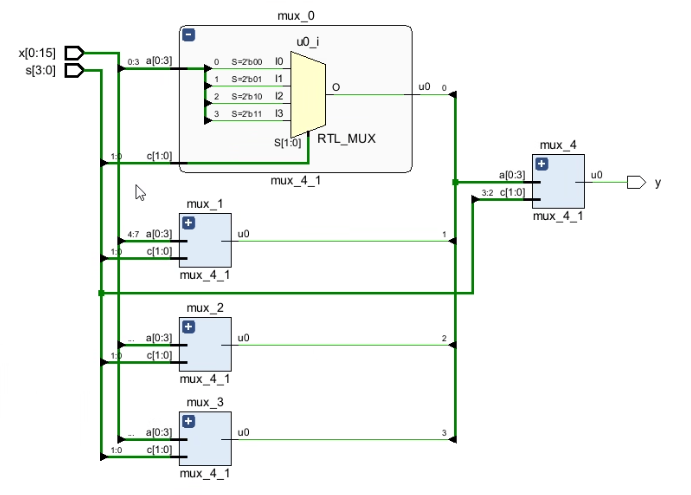
\includegraphics[width=16cm]{immagini/esercizio1/schema_1.1.png}
    \caption{Schema Multiplexer 16:1}
    \label{fig:mux_16_1}
\end{figure}

Il componente fondamentale dell'architettura è il \textit{multiplexer} 4:1 ed è stato realizzato con un approccio comportamentale come descritto nel listato in \ref{mux_4_1} con il costrutto \textit{case-when} inserito in un \textit{process} la cui lista di sensitività contiene sia la selezione che il dato.

\begin{lstlisting}[language=VHDL, label=mux_4_1, caption=Multiplexer 4:1]
library IEEE;
use IEEE.STD_LOGIC_1164.ALL;

entity mux_4_1 is
    Port ( 
        a: in STD_LOGIC_VECTOR (0 to 3);
        c: in STD_LOGIC_VECTOR (1 downto 0);
        u0: out STD_LOGIC
    );
end mux_4_1;

architecture behavioral of mux_4_1 is
begin
    process (a,c)
        begin  
        case c is 
            when "00" => u0 <= a(0);
            when "01" => u0 <= a(1);
            when "10" => u0 <= a(2);
            when "11" => u0 <= a(3);
            when others => u0 <= '-';
        end case;
    end process;
         
end behavioral;
\end{lstlisting}

L'architettura mostrata in Figura \ref{fig:mux_16_1} è stata realizzando componendo i singoli multiplexer, come illustrato nel listato \ref{mux_16_1}. In particolare, gli ingressi sono stati memorizzati in un vettore di $16 bit$ e le selezioni in uno da $4$, mentre l'uscita è rappresentata da un singolo segnale. Ai multiplexer elementari sono assegnati opportunamente i segnali di ingresso, ad esempio: al \textit{mux\_0}, sono stati assegnati i primi $4$ bit; al \textit{mux\_1} i successivi $4$ e così via. 

\begin{lstlisting}[language=VHDL, label=mux_16_1 caption=Multiplexer 16:1]
library IEEE;
use IEEE.STD_LOGIC_1164.ALL;

entity mux_16_1 is
  Port ( 
      x: in STD_LOGIC_VECTOR (0 to 15);
      s: in STD_LOGIC_VECTOR (3 downto 0); 
      y: out STD_LOGIC
  );
end mux_16_1;

architecture structural of mux_16_1 is
   component mux_4_1 is
     Port ( 
        a: in STD_LOGIC_VECTOR (0 to 3);
        c: in STD_LOGIC_VECTOR (1 downto 0);
        u0: out STD_LOGIC
     );
   end component;
signal k : STD_LOGIC_VECTOR (0 to 3);
signal inputs: STD_LOGIC_VECTOR(0 to 15);
signal selections: STD_LOGIC_VECTOR(3 downto 0);
signal output: STD_LOGIC;

begin
 mux_0: mux_4_1 
  Port map(
    a(0 to 3) => x(0 to 3),
    c(1 downto 0) => s(1 downto 0),
    u0=>k(0)  
  );
  
 mux_1: mux_4_1 
  Port map(
    a(0 to 3) => x(4 to 7),
    c(1 downto 0) => s(1 downto 0),
    u0=>k(1)  
  );

 mux_2: mux_4_1 
  Port map(
    a(0 to 3) => x(8 to 11),
    c(1 downto 0) => s(1 downto 0),
    u0=>k(2)  
  );
  
 mux_3: mux_4_1 
  Port map(
    a(0 to 3) => x(12 to 15),
    c(1 downto 0) => s(1 downto 0),
    u0=>k(3)  
  );

  mux_4: mux_4_1
  Port map (
    a(0 to 3) => k(0 to 3),
    c(1 downto 0) => s(3 downto 2),
    u0 => y
  );
   
end structural;
\end{lstlisting}


\subsection{Testing}
Sono stati esaminati due casi di test, in cui con uno stesso segnale di ingresso sono stati fatti variare i bit di controllo. Per ogni test sono stati verificati gli output attesi.
L'input mette a $1$ le linee di ingresso $6,7,8,9$.\\
Per il primo caso di test la selezione è "0110" per cui ci si aspetta correttamente l'output in $1$.\\
Per il secondo caso di test la selezione è "0001" per cui ci si aspetta correttamente l'output pari $0$.

Nel listato \ref{mux_16_1}, è riportato il \textit{testbench} utilizzato per testare il componente realizzato.

\begin{lstlisting}[language=VHDL, label=mux_16_1, caption=Testbench mux 16:4]
library IEEE;
use IEEE.STD_LOGIC_1164.ALL;

entity mux_16_1_TB is
end mux_16_1_TB;

architecture Behavioral of mux_16_1_TB is

  component mux_16_1 is
    Port ( 
      x: in std_logic_vector(0 to 15);
      s: in std_logic_vector(3 downto 0); 
      y: out std_logic
    );
  end component;

signal inputs: std_logic_vector(0 to 15);
signal selections: std_logic_vector(3 downto 0);
signal output: std_logic;

begin
  --Unit Under Test
  uut: mux_16_1
    Port map ( 
      x => inputs,
      s => selections,
      y => output
    );
  test_bench: process
  begin
    -- Caso test 1
    wait for 10 ns;
    inputs <= "0000001111000000";
    selections <= "0110";
    wait for 10 ns;
    assert output <= '1';
    report "errore_1" severity failure;

    -- Caso test 2
    wait for 20 ns;
    inputs <= "0000001111000000";
    selections <= "0001";
    wait for 10 ns;
    assert output <= '0';
    report "errore_2" severity failure;
  wait;
  end process;
end Behavioral;
\end{lstlisting}

\begin{figure}[H]
    \centering
    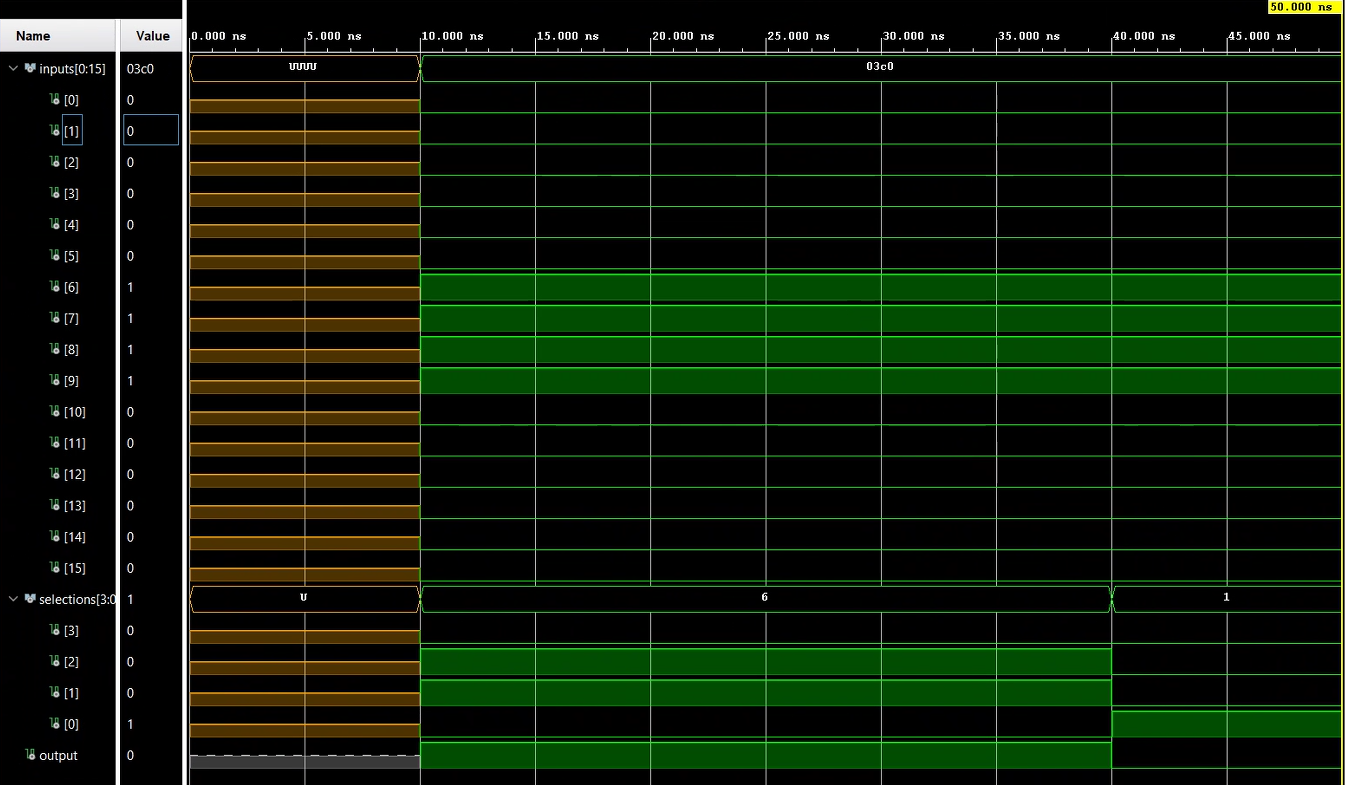
\includegraphics[width=16cm]{immagini/esercizio1/output_simulazione_1.1.png}
    \caption{Simulazione}
    \label{fig:notebook}
\end{figure}

\section{Rete 16:4}
\paragraph{Traccia}
Utilizzando il componente sviluppato al punto precedente, progettare, implementare in VHDL e testare mediante simulazione una rete di interconnessione a 16 sorgenti e 4 destinazioni.

\subsection{Architettura}

Come descritto nello schema in Figura \ref{fig:16_4}, per costruire una rete 16:4 è necessario collegare in cascata un \textit{multiplexer 16:1} e un \textit{de-multiplexer 1:4}  ai quali bisogna assegnare, in maniera opportuna, gli ingressi di selezione. Infatti, al \textit{multiplexer} sono stati assegnati i $4$ bit più significativi del vettore della selezione, mentre al \textit{de-multiplexer} corrispondono i $2$ bit meno significativi. 

L'architettura si presenta come segue:
\begin{figure}[H]
    \centering
    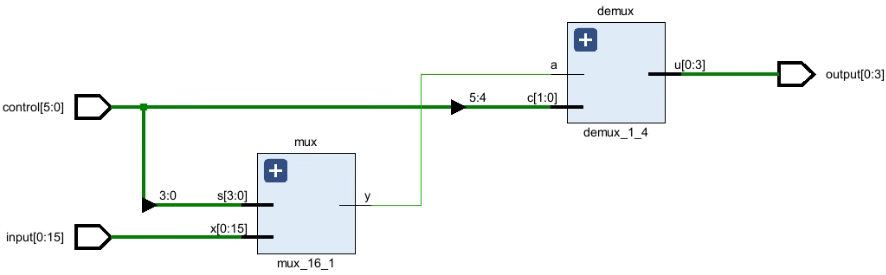
\includegraphics[width=16cm]{immagini/esercizio1/schema_1.2.png}
    \caption{Schema architettura}
    \label{fig:16_4}
\end{figure}

Analogamente al \textit{multiplexer} nel paragrafo precedente, il \textit{de-multiplexer} è implementato in un \textit{process} con il costrutto \textit{case-when}, come illustrato nel listato \ref{demux_1_4}.

\begin{lstlisting}[language=VHDL, label=demux_1_4, caption=Demultiplexer 1:4]
library IEEE;
use IEEE.STD_LOGIC_1164.ALL;

entity demux_1_4 is
    Port (
        a: in STD_LOGIC;
        c: in STD_LOGIC_VECTOR (1 downto 0);
        u: out STD_LOGIC_VECTOR(0 to 3)
    );
end demux_1_4;

architecture Behavioral of demux_1_4 is

begin
    process(a,c)
        begin
        case c is 

        when "00" => 
            u(0) <= a;
            u(1) <= '0';
            u(2) <= '0';
            u(3) <= '0';
        
        when "01" => 
            u(0) <= '0';
            u(1) <= a;
            u(2) <= '0';
            u(3) <= '0';
            
        when "10" => 
            u(0) <= '0';
            u(1) <= '0';
            u(2) <= a;
            u(3) <= '0';
            
        when "11" => 
            u(0) <= '0';
            u(1) <= '0';
            u(2) <= '0';
            u(3) <= a;

        when others => 
            u(0)<= '-';
            u(1)<= '-';
            u(2)<= '-';
            u(3)<= '-';
        end case;
    end process;
end Behavioral;
\end{lstlisting}

Nel listato \ref{rete_16_4} è mostrata l'implementazione della soluzione. In particolare, i due componenti dell'architettura sono collegati mediante il segnale \textit{k}. 

\begin{lstlisting} [language=VHDL, label=rete_16_4, caption=Rete 16:4]
library IEEE;
use IEEE.std_logic_1164.ALL;

entity Rete_16_4 is 
  Port (  
    input: in std_logic_vector(0 to 15);
    control: in std_logic_vector(5 downto 0); 
    output: out std_logic_vector(0 to 3)
  );
end Rete_16_4;

architecture Structural of Rete_16_4 is

  component mux_16_1 is
    Port ( 
      x: in std_logic_vector(0 to 15);
      s: in std_logic_vector(3 downto 0); 
      y: out std_logic
    );
  end component;

  component demux_1_4 is
    Port (
      a: in std_logic;
      c: in std_logic_vector (1 downto 0);
      u: out std_logic_vector(0 to 3)
     );
  end component;

 signal k : std_logic;
 begin
   mux: mux_16_1 port map(
       x(0 to 15) => input(0 to 15),
       s(3 downto 0) => control(3 downto 0),
       y=>k
     );
    
   demux: demux_1_4 port map(
       a => k,
       c(1 downto 0) => control(5 downto 4),
       u(0 to 3)=>output(0 to 3)
     );

 end Structural;
\end{lstlisting}


\subsection{Testing}
Per dimostrare il corretto funzionamento del componente è stato progettato un \textit{testbench} (riportato per intero nel listato \ref{tb_16_4}) con 3 casi di test in cui sono assegnati degli \textit{input} e viene verificato un \textit{assert} con l'\textit{output} atteso. Infine, in Figura \ref{fig:sim_1_2} è mostrata l'esecuzione della testbench mediante una simulazione.

\begin{lstlisting}[language=VHDL, label=tb_16_4, caption=Testbench Rete 16:4]
library IEEE;
use IEEE.STD_LOGIC_1164.ALL;

entity Rete_16_4_TB is
end Rete_16_4_TB;

architecture Behavioral of Rete_16_4_TB is

component Rete_16_4 is
  Port (  
    input: in std_logic_vector(0 to 15);
    control: in std_logic_vector(5 downto 0); 
    output: out std_logic_vector(0 to 3)
  );
end component;

signal inputs_16_4: std_logic_vector(0 to 15);
signal selections_16_4: std_logic_vector(5 downto 0);
signal output_16_4: std_logic_vector(0 to 3);
begin

--Unit Under Test
  uut: Rete_16_4
    Port map ( 
      input=> inputs_16_4,
      control => selections_16_4,
      output => output_16_4
    );

test_bench: process
begin

  wait for 100 ns;

  -- Caso di test 1
  inputs_16_4 <= "0000001111000000";
  selections_16_4 <= "011001";
  wait for 10 ns;
  assert output_16_4(1) = '1' report "errore0" severity failure;

  -- Caso di test 2
  wait for 10 ns;
  inputs_16_4 <= "1111111111111111";
  selections_16_4 <= "111110";
  wait for 10 ns;
  assert output_16_4(3) = '1' report "errore1" severity failure;

  -- Caso di test 3
  wait for 10 ns;
  inputs_16_4 <= "0000001111000000";
  selections_16_4 <= "011001";
  wait for 10 ns;
  assert output_16_4(1) = '0' report "errore2" severity failure;

  wait;

end process;
end Behavioral;
\end{lstlisting}


\begin{figure}[H]
    \centering
    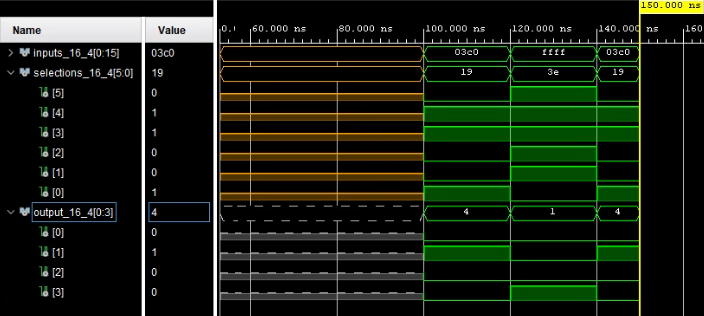
\includegraphics[width=16cm]{immagini/esercizio1/output_simulazione_1_2.png}
    \caption{Simulazione}
    \label{fig:sim_1_2}
\end{figure}



\section{Sintesi su scheda}
\paragraph{Traccia}
Sintetizzare ed implementare su board il progetto della rete di interconnessione sviluppato al punto 1.2, utilizzando gli switch per fornire gli input di selezione e i led per visualizzare i 4 bit di uscita. Per quanto riguarda i 16 bit dato in input, essi possono essere precaricati nel sistema oppure immessi anch’essi mediante switch, sviluppando in questo secondo caso un’apposita rete di controllo per l’acquisizione.

\subsection{Implementazione}
Per la risoluzione dell'esercizio si è deciso di integrare la soluzione precedente. In particolare è stata implementata una rete di controllo, che serve ad effettuare l'acquisizione del dato in ingresso dagli \textit{switch} della scheda e ad avviare la trasmissione con un pulsante.

\subsubsection{Acquisizione dati}
Per acquisire i dati dalla \textit{board} è stata effettuata la mappatura degli \textit{switch} con il vettore dei segnali di ingresso ed è stato integrato l'esercizio 1.2 con una rete di controllo implementata con un FSM (illustrata in Figura \ref{fig:cu_1_3}). Questa introduzione trasforma la macchina da puramente combinatoria a sequenziale, con la necessità di introdurre il \textit{clock}. Inoltre, l'impulso del pulsante fisico deve essere ripulito da un \textit{debouncer} per evitare che duri più di un colpo di \textit{clock}.


\begin{figure}[H]
    \centering
    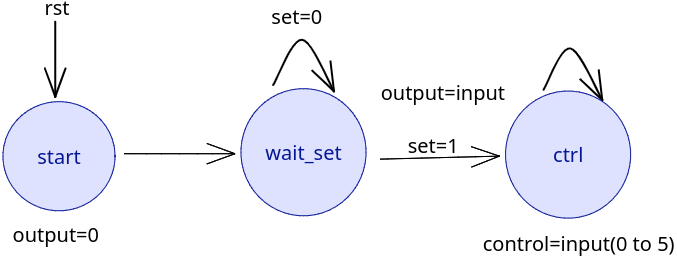
\includegraphics[width=14cm]{immagini/esercizio1/automa_1.3.png}
    \caption{Rete di controllo}
    \label{fig:cu_1_3}
\end{figure}

Nel listato \ref{dbncr} è stata riportata per semplicità solo l'interfaccia utilizzata del componente \textit{ButtonDebouncer}. In particolare, attraverso i parametri di \textit{clock} e tempo di rimbalzo crea un contatore che controlla che la pressione del pulsante sia costante in modo tale da eliminare leggere perturbazioni che potrebbero portare ad avere comportamenti errati.

\begin{lstlisting}[language=VHDL, label=dbncr, caption=Interfaccia ButtonDebouncer]
entity ButtonDebouncer is
   generic(  CLK_period: integer := 10; -- periodo del clock in nanosec
             btn_noise_time: integer := 10000000 --durata dell'oscillazione in nanosec  );
    Port ( RST : in STD_LOGIC;
           CLK : in STD_LOGIC;
           BTN : in STD_LOGIC; 
           CLEARED_BTN : out STD_LOGIC);
end ButtonDebouncer;
\end{lstlisting}
\chapter{Encoder BCD}

\section{Encoder BCD}
\paragraph{Traccia}
Progettare, implementare in VHDL e testare mediante simulazione una rete che, data in ingresso una stringa binaria X di 10 bit X9 X8 X7 X6 X5 X4 X3 X2 X1 X0 che corrisponde alla rappresentazione decodificata di una cifra decimale (cioè, una rappresentazione in cui ogni stringa contiene un solo bit alto), fornisce in uscita la rappresentazione Y della cifra mediante codifica Binary-Coded Decimali (BCD). 

\subsection{Architettura}
L'\textit{encoder} è una macchina combinatoria che realizza una funzione di corrispondenza ben definita tra ingresso e uscita. In Figura \ref{fig:encoder_arch} è mostrata l'architettura della soluzione.

\begin{figure}[H]
    \centering
    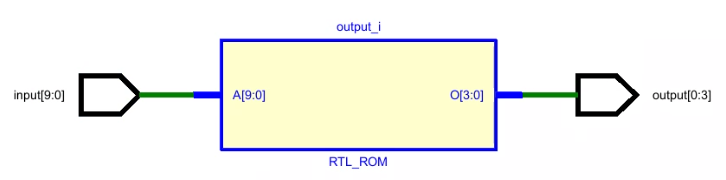
\includegraphics[width=15cm]{immagini/esercizio2/schema_2.1.png}
    \caption{Architettura encoder}
    \label{fig:encoder_arch}
\end{figure}

L'implementazione è stata realizzata mediante un processo con il costrutto \textit{case-when} ed è riportata nel listato \ref{encoder}.

\begin{lstlisting}[language=VHDL, label=encoder, caption=Encoder BCD]
library IEEE;
use IEEE.STD_LOGIC_1164.ALL;
entity encoder is port ( 
    input: in STD_LOGIC_VECTOR (9 downto 0);
    output: out STD_LOGIC_VECTOR (0 to 3)
  );
end encoder;

architecture Behavioral of encoder is

begin
    process(input)
        begin 
        case input is 
            when "0000000001" => output <="0000";
            when "0000000010" => output <="0001";
            when "0000000100" => output <="0010";
            when "0000001000" => output <="0011";
            when "0000010000" => output <="0100";
            when "0000100000" => output <="0101";
            when "0001000000" => output <="0110";
            when "0010000000" => output <="0111";
            when "0100000000" => output <="1000";
            when "1000000000" => output <="1001";
            when others =>output<="----";
            end case;   
    end process;    
end Behavioral;
\end{lstlisting}

\subsection{Testing}
Essendo il numero di input limitato, è stato possibile effettuare un testing esaustivo: ogni input è una stringa che contiene un solo bit alto. Per ogni test sono stati verificati gli output attesi, mentre l'output della simulazione è presente in Figura \ref{fig:Simulazione encoder}
Il \textit{testbench} è presente nel listato \ref{tb_encoder}.
\begin{lstlisting}[language=VHDL, label=tb_encoder, caption=Simulazione encoder]
library IEEE;
use IEEE.STD_LOGIC_1164.ALL;

entity encoder_TB is
end encoder_TB;
architecture Behavioral of encoder_TB is

component encoder is 
    Port(
        input: in STD_LOGIC_VECTOR (9 downto 0);
        output: out STD_LOGIC_VECTOR (0 to 3)
    );
end component;

signal s_input: STD_LOGIC_VECTOR(9 downto 0);
signal s_output: STD_LOGIC_VECTOR(0 to 3);

begin
  uut: encoder
    Port map ( 
      input=>s_input,
      output=>s_output
    );

test_bench: process
begin
    wait for 100 ns;

    s_input<="0000000001";
    wait for 10 ns;
    assert s_output = "0000"
    report "errore";
    wait for 10 ns;

    s_input<="0000000010";
    wait for 10 ns;
    assert  s_output = "0001"
    report "errore 1";
    wait for 10 ns;

    s_input<="0000000100";
    wait for 10 ns;
    assert  s_output = "0010"
    report "errore";
    wait for 10 ns;

    s_input<="0000001000";
    wait for 10 ns;
    assert  s_output = "0011"
    report "errore";
    wait for 10 ns;

    s_input<="0000010000";
    wait for 10 ns;
    assert  s_output = "0100"
    report "errore";
    wait for 10 ns;

    s_input<="0000100000";
    wait for 10 ns;
    assert  s_output = "0101"
    report "errore";
    wait for 10 ns;
    
    s_input<="0001000000";
    wait for 10 ns;
    assert  s_output = "0110"
    report "errore";
    wait for 10 ns;

    s_input<="0010000000";
    wait for 10 ns;
    assert  s_output = "0111"
    report "errore";
    wait for 10 ns;
    
    s_input<="0100000000";
    wait for 10 ns;
    assert  s_output = "1000"
    report "errore";
    wait for 10 ns;

    s_input<="1000000000";
    wait for 10 ns;
    assert  s_output = "1001"
    report "errore";
    wait;
end process;
end Behavioral;
\end{lstlisting}

\begin{figure}[H]
    \centering
    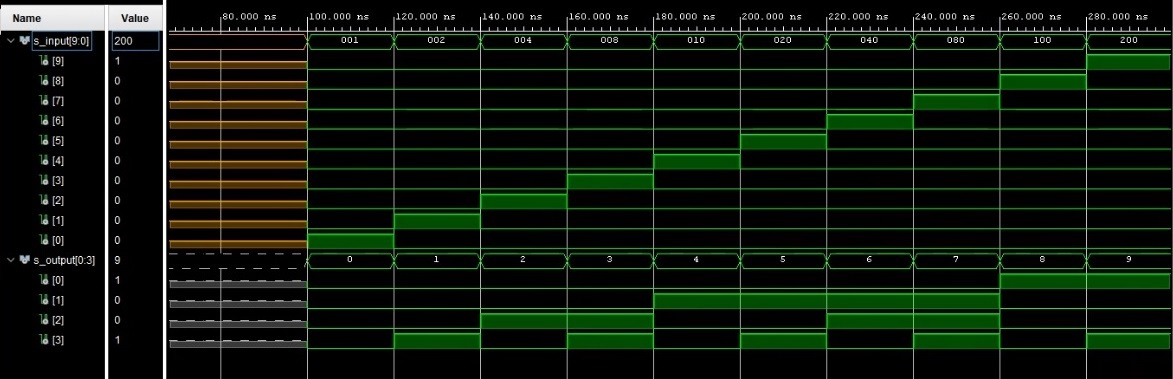
\includegraphics[width=16cm]{immagini/esercizio2/output_simulazione_2.1.jpg}
    \caption{Output della simulazione}
    \label{fig:Simulazione encoder}
\end{figure}

\section{Sintesi su scheda}
\paragraph{Traccia} 
Sintetizzare ed implementare su board il progetto dell’encoder BCD utilizzando gli switch per fornire la stringa X in ingresso, e i led per visualizzare Y. Nel caso in cui si utilizzi una board dotata di soli 8 switch, è possibile sviluppare il progetto considerando X di soli 8 bit (la macchina sarà allora in grado di fornire in uscita la rappresentazione BCD delle cifre decimali da 0 a 7).

\subsection{Implementazione}
In questo caso, la macchina resta completamente combinatoria e, pertanto, sono stati mappati gli switch della scheda direttamente sugli input dell'encoder. Una dimostrazione visiva del risultato è riportata nel file \textit{2.2.mkv} nella sezione materiale multimediale.

\section{Sintesi su scheda}
\paragraph{Traccia}
Utilizzare un display a 7 segmenti per visualizzare la cifra decimale codificata da Y (pilotare opportunamente i catodi del display).

\subsection{Implementazione}
Per la sintesi è stata creata un'unità dedicata \textit{Encoder\_OnBoard} (la cui implementazione è presente nel listato \ref{encoder_on_board}), tale unità utilizza il componente \textit{Encoder} sviluppato in precedenza, e si occupa di interagire con i segnali della scheda. In particolare, viene eseguita l'assegnazione degli input sugli switch della scheda e degli output sul display. Per il display è stato utilizzato il componente \textit{cathod\_manager} la cui interfaccia è riportata nel listato \ref{cathod_manager}.

\begin{lstlisting}[language=VHDL, label=cathod_manager, caption=Interfaccia cathod manager]
entity cathodes_manager is
    Port (
        value : in  STD_LOGIC_VECTOR (3 downto 0); --dato da mostrare sulla cifra del display
        dot : in  STD_LOGIC; --punto
        cathodes_dot : out  STD_LOGIC_VECTOR (7 downto 0)); --indica i 7 catodi + il punto
end cathodes_manager;
\end{lstlisting}

\begin{lstlisting}[language=VHDL, label=encoder_on_board, caption=Implementazione Encoder\_OnBoard]
library IEEE;
use IEEE.STD_LOGIC_1164.ALL;

entity Encoder_onBoard is
    Port (
        input : in STD_LOGIC_VECTOR(9 downto 0);
        led : out STD_LOGIC_VECTOR(3 downto 0);
        catodi : out STD_LOGIC_VECTOR(7 downto 0);
        anodi : out STD_LOGIC_VECTOR(7 downto 0)
    );
end Encoder_onBoard;

architecture Behavioral of Encoder_onBoard is

   component encoder
       Port (
         input: in STD_LOGIC_VECTOR (9 downto 0);
         output: out STD_LOGIC_VECTOR (3 downto 0)
       );
   end component;


   component cathodes_manager
       Port(
          value : in std_logic_vector(3 downto 0);
          dot : in std_logic;
          cathodes_dot : out std_logic_vector(7 downto 0)
       );
   end component;

    signal ytemp : std_logic_vector (3 downto 0);
    signal dot : std_logic;
    
begin

    dot <= '1';  --decido di voler illuminare il punto accanto alla cifra
    anodi <=(others=>'0'); --decido di voler illuminare tutte le cifre dei due display (anodi 0-attivi)
    led <= ytemp;

    enc: Encoder port map(
            input => input,
            output => ytemp
        );

    cat: cathodes_manager port map(
            value => ytemp,
            dot => dot,
            cathodes_dot => catodi
        );

end Behavioral;
\end{lstlisting}
\chapter{Riconoscitore di sequenze}

\section{Riconoscitore di sequenze}
\paragraph{Traccia}
Progettare, implementare in VHDL e testare mediante simulazione una macchina in grado di riconoscere la sequenza 1001. La macchina prende in ingresso un segnale binario i che rappresenta il dato, un segnale A di tempificazione e un segnale M di modo, che ne disciplina il funzionamento, e fornisce un’uscita Y alta quando la sequenza viene riconosciuta. In particolare, 
-	se M=0, la macchina valuta i bit seriali in ingresso a gruppi di 4, 
-	se M=1, la macchina valuta i bit seriali in ingresso uno alla volta, tornando allo stato iniziale ogni volta che la sequenza viene correttamente riconosciuta.


\subsection{Architettura}
Data la natura sequenziale del problema è stato realizzato un automa a stati finiti di cui è possibile vedere lo schema in Figura \ref{fig: automa_3.1}.

\begin{figure}[H]
    \centering
    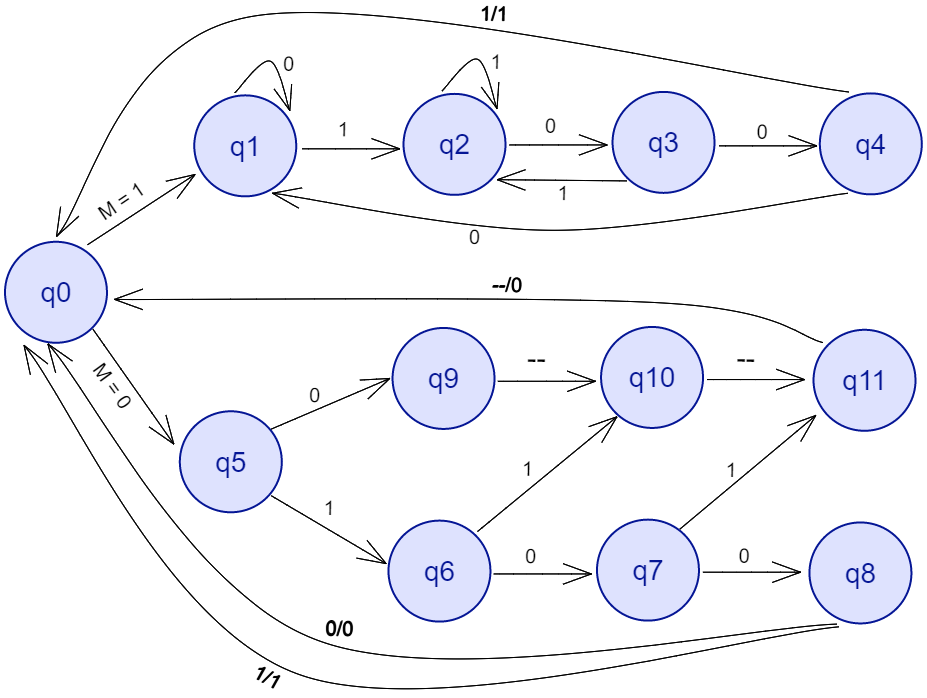
\includegraphics[width=14cm]{immagini/esercizio3/schema_3.1.png}
    \caption{Schema della soluzione}
    \label{fig: automa_3.1}
\end{figure}


Essendo una macchina sequenziale, è stato descritto il funzionamento dell'automa, dividendo la parte combinatoria da quella sequenziale. È stato esaminato il comportamento della macchina in ogni stato, in base agli input e, inoltre, è stato descritto il funzionamento del clock.
La macchina può funzionare in due diverse modalità, rappresentate dalle diramazioni che partono dagli stati \textbf{$q_1$} e \textbf{$q_5$}. Per poter scegliere tra le due si imposta il \textbf{modo} M nel primo stato \textbf{$q_0$}. É da notare che è possibile cambiare il modo solamente partendo da \textbf{$q_0$}, per cui si hanno due opzioni: o si aspetta che la sequenza venga riconosciuta e quindi si torna a \textbf{$q_0$} auromanticamente, oppure è necessario utilizzare il segnale di \textbf{reset}. Questo comportamento è stato scelto in modo da garantire l'integrità del riconoscimento una volta avviato, e inoltre permette di semplificare la logica interna agli stati non dovendo gestire sempre il modo.

 L'implementazione dell'automa, nel listato di codice \ref{riconoscitore_sequenza}, prevede la separazione della componente combinatoria, quella che sceglie in quale stato andare in base agli input e imposta gli output, da quella sequenziale, che si occupa dell'effettivo cambio di stato. 
 Sono infatti presenti due processi diversi. Nel primo viene utilizzato il costrutto \textit{case when} per definire gli stati e i possibili input, per cui la \textit{sensitivity list} comprende lo stato corrente e i dati in ingresso. Il secondo è invece attivato solo dal clock, presente nella sensitivity list, ed a ogni fronte di salita cambia lo stato corrente con il prossimo. É stato utilizzato un reset sincrono, infatti il segnale di reset è assente dalla lista di sensitività. In questo modo il reset allo stato \textit{$s_0$} avverrà in maniera sincronizzata con il clock.
\begin{lstlisting} [language=VHDL, label=riconoscitore_sequenza, caption=Riconoscitore di sequenze]
library IEEE;
use IEEE.STD_LOGIC_1164.ALL;

entity riconoscitore_sequenza is
    Port(
        i: in std_logic;
        A: in std_logic;
        RST: in std_logic;
        M: in std_logic; 
        Y: out std_logic          
    );
end riconoscitore_sequenza;

architecture Behavioral of riconoscitore_sequenza is

type stato is (S0, S1, S2, S3, S4, S5, S6, S7, S8, S9, S10, S11);
signal stato_corrente : stato:= S0;
signal stato_prossimo : stato;

begin

  f_stato_uscita: process(stato_corrente,i) 
    begin
    case stato_corrente is 
    
        when S0=>
            if(M='0') then
                stato_prossimo<=S5;
                Y<='0';
            else
                stato_prossimo<=S1;
                Y<='0';
            end if;
    
        when S1=>
            if(i='0') then
                stato_prossimo<=S1;
                Y<='0';
            else
                stato_prossimo<=S2;
                Y<='0';
            end if;
    
         when S2=>
            if(i='0') then
                stato_prossimo<=S3;
                Y<='0';
            else
                stato_prossimo<=S2;
                Y<='0';
            end if;   

         when S3=>
            if(i='0') then
                stato_prossimo<=S4;
                Y<='0';
            else
                stato_prossimo<=S2;
                Y<='0';
            end if;   

         when S4=>
            if(i='0') then
                stato_prossimo<=S1;
                Y<='0';
            else
                stato_prossimo<=S0;
                Y<='1';
            end if;        
            
         when S5=>
            if(i='0') then
                stato_prossimo<=S9;
                Y<='0';
            else
                stato_prossimo<=S6;
                Y<='0';
            end if;               
    
         when S6=>
            if(i='0') then
                stato_prossimo<=S7;
                Y<='0';
            else
                stato_prossimo<=S10;
                Y<='0';
            end if;       
    
          when S7=>
            if(i='0') then
                stato_prossimo<=S8;
                Y<='0';
            else
                stato_prossimo<=S11;
                Y<='0';
            end if;      
    
          when S8=>
            if(i='0') then
                stato_prossimo<=S0;
                Y<='0';
            else
                stato_prossimo<=S0;
                Y<='1';
            end if;      
    
          when S9=>
            if(i='0') then
                stato_prossimo<=S10;
                Y<='0';
            else
                stato_prossimo<=S10;
                Y<='0';
            end if;      
    
           when S10=>
            if(i='0') then
                stato_prossimo<=S11;
                Y<='0';
            else
                stato_prossimo<=S11;
                Y<='0';
            end if;   
    
           when S11=>
            if(i='0') then
                stato_prossimo<=S0;
                Y<='0';
            else
                stato_prossimo<=S0;
                Y<='0';
            end if;     
        end case;
    end process;
    
    mem: process(A)
    begin 
        if (A'event and A='1') then
            if(RST='1')then 
                stato_corrente<=S0;
            else
            stato_corrente<=stato_prossimo;  
            end if;
        end if;
    end process;
end Behavioral;
\end{lstlisting}

\subsection{Testing}

In primo luogo è stata effettuata una wait di 100 ns per aspettare che il segnale di GRS (Global Set Reset) diventasse alto ed è stata resettata la macchina. Sono stati verificati quattro casi di test.
I primi tre casi di test sono stati effettuati impostando il modo a 0, ovvero riconoscendo la sequenza a gruppi di 4. Nel primo è stato inserito in input la sequenza corretta, negli altri due la sequenza errata. In particolare, la sequenza errata è stata inserita in modo che il sistema fosse in grado di riconoscere lo stato errato della modalità 1. 
Infine, l'ultimo caso di test è stato effettuato impostando il modo a 1, ovvero il sistema deve essere in grado di riconoscere la sequenza all'interno di un generico blocco. Dopo una serie di bit errati misti a quelli corretti si giunge al riconoscimento. All'interno della schermata di simulazione sono stati aggiunti gli stati prossimi e correnti dell'automa, in modo da tracciarne l'evoluzione.

I casi di test sono stati realizzati con il seguente codice:

\begin{lstlisting} [language=VHDL, caption=Testbench example]
library IEEE;
use IEEE.STD_LOGIC_1164.ALL;

entity riconoscitore_sequenza_TB is
end riconoscitore_sequenza_TB;

architecture Behavioral of riconoscitore_sequenza_TB is

    component riconoscitore_sequenza is
        Port(
            i: in std_logic;
            A: in std_logic;
            RST: in std_logic;
            M: in std_logic;
            Y: out std_logic
        );
    end component;

    signal input: std_logic:= '0';
    signal clock: std_logic:= '0';
    signal reset: std_logic:= '0';
    signal mode: std_logic:= '0';
    signal output: std_logic;
    constant CLK_period : time := 10 ns;

begin
    uut: riconoscitore_sequenza
        port map(
            i=>input,
            A=>clock,
            RST=>reset,
            M=>mode,
            Y=>output
        );

    CLK: process
    begin
        clock<='0';
        wait for CLK_period/2;
        clock<='1';
        wait for CLK_period/2;
    end process;

    RS_TB: process
    begin
        wait for 100 ns;
        reset<='1';
        wait for 10 ns;
        reset<='0';

        mode<='0'; 
        -- Caso di test 1
        wait for 10ns;
        input<='1';
        wait for 10ns;
        input<='0';
        wait for 10ns;
        input<='0';
        wait for 10ns;
        input<='1';
        wait for 5ns;
        assert output='1' 
        report "errore modo 0 caso 1";
        wait for 5ns;

        -- Caso di test 2
        input<='1';
        wait for 10ns;
        input<='1';
        wait for 10ns;
        input<='0';
        wait for 10ns;
        input<='0';
        wait for 10ns;
        input<='0';
        wait for 5ns;
        assert output='0'
        report "errore modo 0 caso 2";
        wait for 5ns;

        --Caso di test 3
        input<='1';
        wait for 10ns;
        input<='1';
        wait for 10ns;
        input<='1';
        wait for 10ns;
        input<='1';
        wait for 10ns;
        
        mode<='1';
        -- Caso di test 4
        wait for 10ns;
        input<='1';
        wait for 10ns;
        input<='1';
        wait for 10ns;
        input<='0';
        wait for 10ns;
        input<='0';
        wait for 10ns;
        input<='1';
        wait for 5ns;
        assert output='1'
        report "errore modo 1 caso 3";
        wait for 5ns;
        
        wait;
    end process;
end Behavioral;
\end{lstlisting}

\begin{figure}[H]
    \centering
    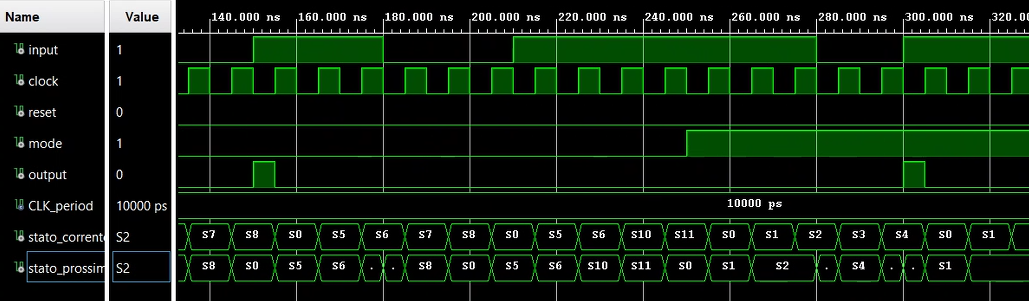
\includegraphics[width=16cm]{immagini/esercizio3/output_simulazione_3.1.png}
    \caption{Output della simulazione}
\end{figure}


\section{Sintesi su scheda}
\paragraph{Traccia}
Sintetizzare e implementare su board la rete sviluppata al punto precedente, utilizzando uno switch S1 per codificare l’input i e uno switch S2 per codificare il modo M, in combinazione con due bottoni B1 e B2 utilizzati rispettivamente per acquisire l’input da S1 e S2 in sincronismo con il segnale di tempificazione A, che deve essere ottenuto a partire dal clock della board. Infine, l’uscita Y può essere codificata utilizzando un led.

\subsection{Implementazione}
Per poter sintetizzare e implementare sulla board la soluzione simulata è stato innanzitutto necessario gestire gli input provenienti dai bottoni. Per farlo sono stati utilizzati due \textit{debouncer}, impostati entrambi con il clock della scheda. Per fornire a tutti i componenti il clock reale del dispositivo sono state decommentate le due righe opportune sul file dei costraint, specificando il nome del segnale utilizzato. La scheda fornisce un clock di 100Mhz, come descritto nei capitoli precedenti, i debouncer "puliscono" i segnali in entrata dai pulsanti in modo che possano essere letti correttamente dai componenti del sistema . Infine sono stati mappati il primo switch all'input e il primo led all'uscita. 
Nel file \textit{video 3.2} presente nel materiale multimediale è possibile vedere il funzionamento della scheda con un caso di test. In particolare, viene impostata in modalità 1 e viene inserita la sequenza corretta da riconoscere. 

Di seguito è mostrato il codice relativo al componente che ingloba tutti gli altri per la sintetizzazione sulla scheda.
È stato utilizzato il riferimento diretto al file sorgente senza l'uso del component.


\begin{lstlisting} [language=VHDL, caption=Testbench example]
library IEEE;
use IEEE.STD_LOGIC_1164.ALL;

entity top_scheda is
    port(
        x      : in std_logic;
        clk    : in std_logic;
        rst    : in std_logic;
        mode     : in std_logic;
        set_mode: in std_logic;
        set_x: in std_logic;
        y    : out std_logic
    );
end top_scheda;

architecture Behavioral of top_scheda is
    signal seq_en: std_logic := '0';
    signal db_set_m, db_set_x : std_logic := '0';
begin

   seq_r: entity work.riconoscitore_sequenza port map(
            clk=>clk,
            en => seq_en,
            rst => rst,
            mode=>mode,
            y=>y,
            x=>x
        );
    
    ctrl_unit: entity work.cu port map (
        clk => clk,
        rst =>rst,
        set_mode=> db_set_m,
        set_x => db_set_x,
        seq_en => seq_en
    );
    dbnc_set_m: entity work.debouncer port map (
        clk=>clk,
        rst=>rst,
        btn=>set_mode,
        cleared_btn => db_set_m
    );
    
      dbnc_set_x: entity work.debouncer port map (
        clk=>clk,
        rst=>rst,
        btn=>set_x,
        cleared_btn => db_set_x
    );

end Behavioral;
\end{lstlisting}
\chapter{Shift register}

\section{Shift register}
\paragraph{Traccia}
Progettare, implementare in VHDL e testare mediante simulazione un registro a scorrimento di N bit in grado di shiftare a destra o a sinistra di un numero Y variabile di posizioni a seconda di una opportuna selezione. Il componente deve essere realizzato utilizzando sia un a) approccio comportamentale sia un b) approccio strutturale.  
Nota: il numero di bit del registro X e i valori che può assumere il parametro Y possono essere scelti dallo studente (ad es. X=8 e Y= {1,2}).

\section{Soluzione Comportamentale}
\subsection{Architettura}
Per l'implementazione della soluzione è stato implementato un sistema che riceve i seguenti segnali di ingresso:
\begin{itemize}
\item \textit{input} è un vettore di 2 bit, che rappresenta gli ingressi che vengono inseriti nel registro;
\item \textit{clock} è il segnale per la tempificazione;
\item \textit{reset} è un segnale per resettare la macchina e farla partire da uno stato noto;
\item \textit{direction} indica il verso di shift, nel programma è stato assunto come ipotesi che il valore direction=0 indichi uno shift verso destra e direction=1 indichi uno shift verso sinistra;
\item \textit{y} è la variabile che indica il numero di shift che è possibile effettuare, in particolare è stato definito come Y=0 lo shift di un solo bit per volta e Y=1 lo shift di due bit per volta;
\end{itemize}

Il sistema presenta il seguente segnale di uscita:
\begin{itemize}
\item \textit{output} è un vettore di 4 bit che rappresenta i valori contenuti nei singoli registri.
\end{itemize}

 È previsto che l'utente debba inserire due bit per controllare il dispositivo, un bit per selezionare il verso di shift e un bit per selezionare il numero di shift. Per ipotesi si assume che nel caso di y=0 (1 solo shift) il comportamento dello shift register è di tipo SIPO (Single Input Parallel Output), mentre per y=1 (2 shift per volta) si assume che il comportamento dello shift regiser è di tipo PIPO (Parallel Input Parallel Output). Per realizzare queste distinzioni di comportamento sono state definite diverse selezioni, al cui intero avviene propagazione dei bit tramite i segnali s1,s2,s3 e s4. Il reset è stato realizzato in modalità sincrona.
 
 Data la possibilità che il sistema scorra di due posizioni è stato deciso di predisporre un ingresso dati di due bit. Durante la modalità y=0 a un solo shift viene letto solo il bit meno significativo, che viene inserito in s1, mentre con y=1 vengono letti entrambi, e vengono inseriti in s1 e s2. Senza questa modifica all'input, nel caso dello shift doppio, si avrebbe una duplicazione del dato. È però importante prendere solo un bit durante lo shift singolo, altrimenti si avrebbe un problema si sovrascrizione come mostrato in Figura \ref{fig:errore}.
 
\begin{figure}[H]
    \centering
    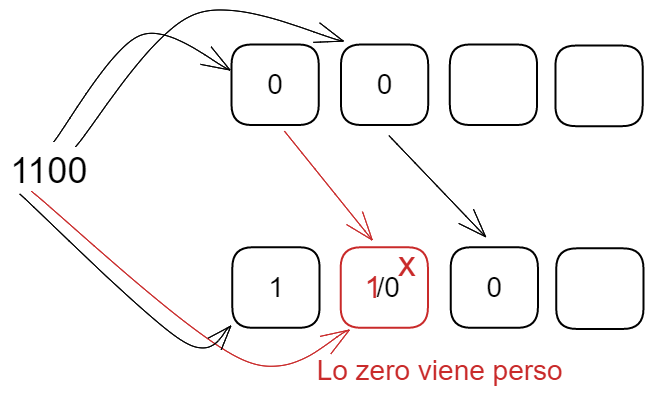
\includegraphics[width=11cm]{immagini/esercizio4/errore.png}
    \caption{Errore}
    \label{fig:errore}
\end{figure}
 
 
La realizzazione tramite approccio comportamentale è stata implementata mediante il seguente codice:
\begin{lstlisting} [language=VHDL, caption=Shift register (Behavioural)]
library IEEE;
use IEEE.STD_LOGIC_1164.ALL;

entity shift_reg_behavioural is
    Port (
        input: in std_logic_vector (1 downto 0);
        clock: in std_logic ;
        reset: in std_logic ;
        direction: in std_logic ; -- 0 shifta a destra, 1 shifta a sinistra
        y: in std_logic; --se Y=0 shift da 1, se Y=1 shift da 2
        output: out std_logic_vector (3 downto 0)
    );
end shift_reg_behavioural;

architecture Behavioral of shift_reg_behavioural is
    signal s1,s2,s3,s4 : std_logic;
begin
    process (clock)
    begin
        if (rising_edge (clock)) then
            if ( reset='1') then
                s1<='0';
                s2<='0';
                s3<='0';
                s4<='0';
            else
                if(y='0') then
                    if(direction ='0') then
                        --destra
                        s1<=input(0) ;
                        s2<=s1;
                        s3<=s2;
                        s4<=s3;

                    elsif (direction ='1') then
                        --sinistra
                        s4<=input(0) ;
                        s3<=s4;
                        s2<=s3;
                        s1<=s2;
                    end if;

                elsif (y='1') then
                    if(direction ='0') then
                        --destra
                        s1<=input(1);
                        s2<=input(0);
                        s3<=s1;
                        s4<=s2;

                    elsif (direction ='1') then
                        --sinistra
                        s4<=input(1);
                        s3<=input(0);
                        s2<=s4;
                        s1<=s3;
                    end if;
                end if;
           end if;
        end if;
    end process;

output<= s1 & s2 & s3 & s4;

end Behavioral;
\end{lstlisting}

\subsection{Simulazione}
In primo luogo è stata effettuata una wait di 100 ns per aspettare che il segnale di GRS (Global Set Reset) diventasse alto ed è stata resettata la macchina. Sono stati effettuati quattro casi di test.
I primi due sono stati verificati sfruttando gli stessi input, impostando Y=0 (effettuando uno shift per volta), facendo variare unicamente la direzione da 0 a 1 (da destra a sinistra).
In modo duale sono stati verificati gli altri due casi di test, impostando Y=1 (effettuando due shift per volta).

\paragraph{Testbench}

\begin{lstlisting} [language=VHDL, caption=Testbench a example]
library IEEE;
use IEEE.STD_LOGIC_1164.ALL;

entity shift_ref_behavioural_TB is
end shift_ref_behavioural_TB;

architecture Behavioral of shift_ref_behavioural_TB is

    component shift_reg_behavioural is
        Port (
            input: in std_logic_vector (1 downto 0);
            clock: in std_logic ;
            reset: in std_logic ;
            direction: in std_logic ; -- 0 shifta a destra, 1 shifta a sinistra
            y: in std_logic; --se Y=0 shift da 1, se Y=1 shift da 2
            output: out std_logic_vector (3 downto 0)
        );

    end component  shift_reg_behavioural;

  signal s_input: std_logic_vector (1 downto 0):=(others => '0');
  signal s_output: std_logic_vector (3 downto 0):=(others => '0');
  signal s_clock, s_reset, s_direction,s_y: std_logic := '0';
  constant clk_period: time := 10 ns;

begin
    uut: shift_reg_behavioural
        port map(
            input=>s_input ,
            output=>s_output,
            clock=>s_clock,
            reset=>s_reset,
            direction=>s_direction,
            y=>s_y
        );

    clock: process
    begin
        s_clock <= '1';
        wait for clk_period/2;
        s_clock <= '0';
        wait for clk_period/2;
    end process clock;

    TB: process
    begin
        wait for 100ns;
        s_reset <='1';
        wait for clk_period;
        s_reset <='0';

        -- Caso di test 1 (Y=0, direction=0)
        s_y <='0';
        s_input<="01";
        wait for clk_period;
        assert (s_output = "1000") report "ERRORE";

        s_input<="00";
        wait for clk_period;
        assert (s_output = "0100") report "ERRORE";

        s_input<="00";
        wait for clk_period;
        assert (s_output = "0010") report "ERRORE";

        s_input<="01";
        wait for clk_period;
        assert (s_output = "1001") report "ERRORE";

        -- Caso di test 2 (Y=0, direction=1)
        s_y <='0';
        s_direction <='1';
        s_reset<='1';
        wait for clk_period;
        s_reset<='0';

        s_input<="01";
        wait for clk_period;
        assert (s_output = "0001") report "ERRORE";

        s_input<="00";
        wait for clk_period;
        assert (s_output = "0010") report "ERRORE";

        s_input<="00";
        wait for clk_period;
        assert (s_output = "0100") report "ERRORE";

        s_input<="01";
        wait for clk_period;
        assert (s_output = "1001") report "ERRORE";

        -- Caso di test 1 (Y=1, direction=0)
        s_y <='1';
        s_direction <='0';
        s_reset<='1';
        wait for clk_period;
        s_reset<='0';

        s_input<="11";
        wait for clk_period;
        assert (s_output = "1100") report "ERRORE";

        s_input<="00";
        wait for clk_period;
        assert (s_output = "0011") report "ERRORE";

        s_input<="11";
        wait for clk_period;
        assert (s_output = "1100") report "ERRORE";

        s_input<="01";
        wait for clk_period;
        assert (s_output = "0111") report "ERRORE";

        -- Caso di test 4 (Y=1, direction=1)
        s_y <='1';
        s_direction <='1';
        s_reset<='1';
        wait for clk_period;
        s_reset<='0';

        s_input<="11";
        wait for clk_period;
        assert (s_output = "0011") report "ERRORE";

        s_input<="00";
        wait for clk_period;
        assert (s_output = "1100") report "ERRORE";

        s_input<="11";
        wait for clk_period;
        assert (s_output = "0011") report "ERRORE";

        s_input<="01";
        wait for clk_period;
        assert (s_output = "1110") report "ERRORE";

        wait;
    end process;
end Behavioral;
\end{lstlisting}


\begin{figure}[H]
    \centering
    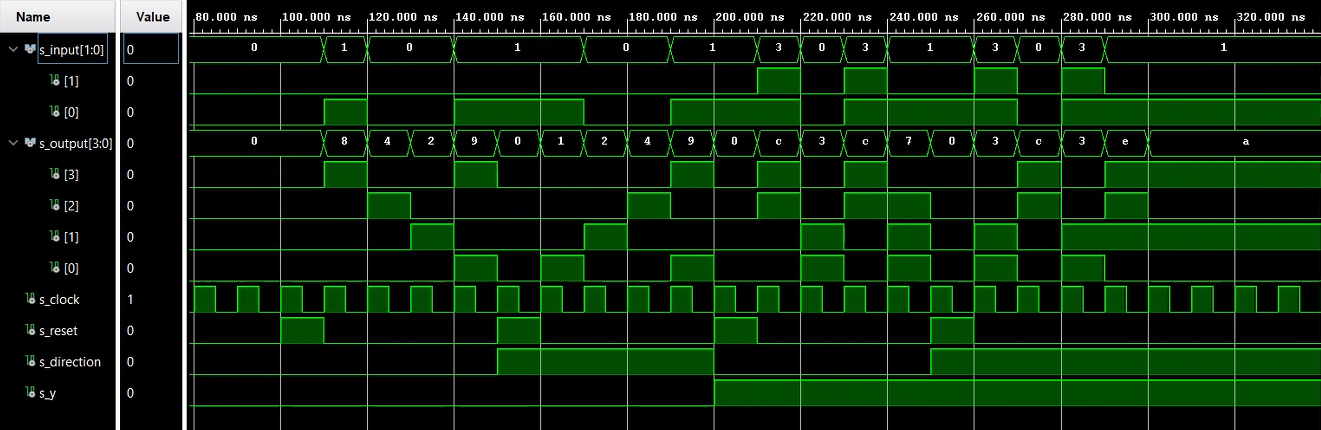
\includegraphics[width=16cm]{immagini/esercizio4/output_simulazione_4.1.png}
    \caption{Output della simulazione}
    \label{fig:notebook}
\end{figure}

\section{Soluzione Strutturale}
\subsection{Architettura}
Il sistema è stato realizzato seguendo un approccio strutturale. In primo luogo sono stati realizzati dei flip flop edge triggered da 1 bit con un semplice processo. Data la complessità dei comandi disponibili dall'utente, si è scelto di realizzare una rete di controllo che gestisce i flip flop e la comunicazione tra essi. Sarebbe stato possibile anche mappare gli input di controllo a una serie di multiplexer in modo da non utilizzare processi, e rendere il sistema più scalabile, ma date le dimensioni ridotte richieste si è scelto un compromesso tra performance e complessità.
La rete di controllo prende in input le uscite dei registri e le smista , tramite il suo output, alle entrate degli stessi, cambiando i flussi dei dati a seconda della modalità. Per fare ciò vengono utilizzati 8 segnali. 
È da notare che mentre i flip flop si attivano sul fronte di discesa del clock, la rete di controllo lo fa su quello di salita. In questo modo, in un singolo colpo di clock, entrambi i componenti possono funzionare senza la creazione di delay causati dall'invio e dalla ricezione dei segnali. In entrambi i componenti si è utilizzato un reset sincrono.

L'architettura si presenta come segue:
\begin{figure}[H]
    \centering
    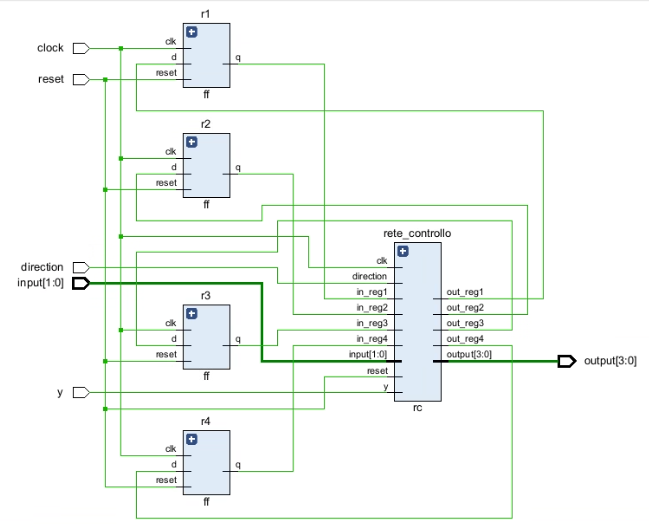
\includegraphics[width=17cm]{immagini/esercizio4/schema_4.2.png}
    \caption{Schema architettura}
    \label{fig:notebook}
\end{figure}

Il componente flip flop è stato realizzato mediante il seguente codice:

\begin{lstlisting}[language=VHDL, caption=flip flop]
library IEEE;
use IEEE.STD_LOGIC_1164.ALL;

entity ff is
    Port (
        d, clk, reset: in std_logic ;
        q: out std_logic );
end ff;
architecture Behavioral of ff is
begin
    process (clk)
    begin
        if falling_edge(clk) then
            if (reset='1') then
                q<='0';
            else
                q<=d;
            end if;
        end if;
    end process;
end Behavioral;
\end{lstlisting}

La rete di controllo è stata realizzata mediante il seguente codice:

\begin{lstlisting}[language=VHDL, caption=Rete di controllo]
library IEEE;
use IEEE.STD_LOGIC_1164.ALL;

entity rc is
    Port (
        input: in std_logic_vector (1 downto 0);
        clk, reset , direction , y: in std_logic ;
        in_reg1, in_reg2, in_reg3, in_reg4: in std_logic;
        out_reg1,out_reg2,out_reg3, out_reg4:out std_logic;
        output: out std_logic_vector (3 downto 0)
    );
end rc;

architecture Behavioral of rc is

begin
    process (clk)
    begin
        if (rising_edge (clk)) then
            if ( reset='1') then
                out_reg1 <='0';
                out_reg2 <='0';
                out_reg3 <='0';
                out_reg4 <='0';

            else
                if(y='0') then
                    if(direction ='0') then
                        --destra
                        out_reg1<=input(0);
                        out_reg2<=in_reg1;
                        out_reg3<=in_reg2;
                        out_reg4<=in_reg3;

                    elsif (direction ='1') then
                        --sinitra
                        out_reg4<=input(0) ;
                        out_reg3<=in_reg4;
                        out_reg2<=in_reg3;
                        out_reg1<=in_reg2;
                    end if;

                elsif (y='1') then
                    if(direction ='0') then
                        --destra
                        out_reg1<=input(1);
                        out_reg2<=input(0);
                        out_reg3<=in_reg1;
                        out_reg4<=in_reg2;

                    elsif (direction ='1') then
                        --sinitra
                        out_reg4<=input(1);
                        out_reg3<=input(0);
                        out_reg2<=in_reg4;
                        out_reg1<=in_reg3;
                    end if;
                end if;
            end if;
        end if;
    end process;
    
    output<=in_reg1 & in_reg2 & in_reg3 & in_reg4;

end Behavioral;
\end{lstlisting}

Lo shift register è stato generato tramite il collegamento degli opportuni componenti: 4 flip-flop e 1 rete di controllo:
\begin{lstlisting} [language=VHDL, caption=Shift Register (Structural)]
library IEEE;
use IEEE.STD_LOGIC_1164.ALL;

entity shift_register is
    Port (
        input: in std_logic_vector (1 downto 0);
        clock: in std_logic ;
        reset: in std_logic ;
        direction: in std_logic ; -- 0 shifta a destra, 1 shifta a sinistra
        y: in std_logic; --se Y=0 shift da 1, se Y=1 shift da 2
        output: out std_logic_vector (3 downto 0)
    );
end shift_register;

architecture Structural of shift_register is

    component ff is port (
        d, clk, reset: in std_logic ;
        q: out std_logic 
     );
    end component ff;

    component  rc is port (
          input: in std_logic_vector (1 downto 0);
          clk, reset , direction , y: in std_logic ;
          in_reg1, in_reg2, in_reg3, in_reg4: in std_logic;
          out_reg1,out_reg2,out_reg3, out_reg4:out std_logic;
          output: out std_logic_vector (3 downto 0)
        );
    end component rc;

    signal s_in_reg1,  s_in_reg2,  s_in_reg3,  s_in_reg4 : std_logic:='0';
    signal s_out_reg1, s_out_reg2, s_out_reg3,  s_out_reg4: std_logic:='0';
    signal s_output: std_logic_vector (3 downto 0);

begin

    r1: ff  port map(
            d=>s_out_reg1,
            clk=> clock,
            reset=> reset,
            q => s_in_reg1 );

    r2: ff  port map(
            d=>s_out_reg2,
            clk=> clock,
            reset=> reset,
            q => s_in_reg2 );

    r3: ff  port map(
            d=>s_out_reg3,
            clk=> clock,
            reset=> reset,
            q => s_in_reg3 );

    r4: ff  port map(
            d=>s_out_reg4,
            clk=> clock,
            reset=> reset,
            q => s_in_reg4 );

    rete_controllo: rc  port map(
            input=> input,
            clk=> clock,
            reset=> reset,
            direction=> direction,
            y=> y,
            in_reg1=> s_in_reg1,
            in_reg2=> s_in_reg2,
            in_reg3=> s_in_reg3,
            in_reg4=> s_in_reg4,

            out_reg1=> s_out_reg1,
            out_reg2=> s_out_reg2,
            out_reg3=> s_out_reg3,
            out_reg4=> s_out_reg4,
            output=>s_output );
        
        output<=s_output;
        
end Structural;
\end{lstlisting}

\subsection{Simulazione}
Il testing di questa rete è stato effettuato con lo stesso testbench che è stato utilizzato nell'approccio comportamentale, che quindi per semplicità viene omesso, avendo dichiarato volutamente gli stessi input e output dell'intera rete. È stato possibile confrontare i due risultati e constatare il corretto funzionamento di entrambi. 

L'output che deriva dal testbench è il seguente:
\begin{figure}[H]
    \centering
    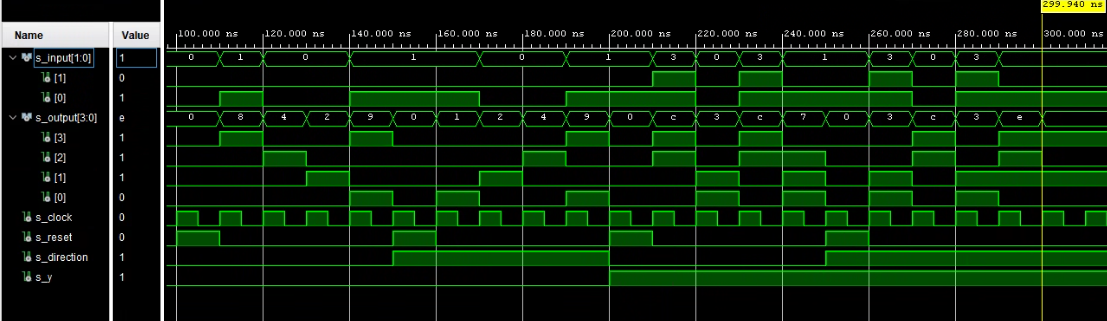
\includegraphics[width=16cm]{immagini/esercizio4/output_simulazione_4.2.png}
    \caption{Output della simulazione}
    \label{fig:notebook}
\end{figure}
\chapter{Cronometro}

\section{Cronometro}
\paragraph{Traccia}
Progettare, implementare in VHDL e testare mediante simulazione un cronometro, in grado di scandire secondi, minuti e ore a partire da una base dei tempi prefissata (es. si consideri il clock a disposizione sulla board). Il progetto deve prevedere la possibilità di inizializzare il cronometro con un valore iniziale, sempre espresso in termini di ore, minuti e secondi, mediante un opportuno ingresso di set, e deve prevedere un ingresso di \textit{reset} per azzerare il tempo.
Il componente deve essere realizzato utilizzando un approccio strutturale, collegando opportunamente dei contatori secondo uno schema a scelta. 

\subsection{Architettura}

Il sistema, realizzato con un approccio strutturale, comprende quattro componenti principali. In particolare, sono stati adibiti tre contatori per il conteggio dei secondi, minuti e ore, mentre il quarto componente è un divisore di frequenza. 

Le interconnessioni tra i componenti sono visibili nella seguente architettura: 
\begin{figure}[H]
    \centering
    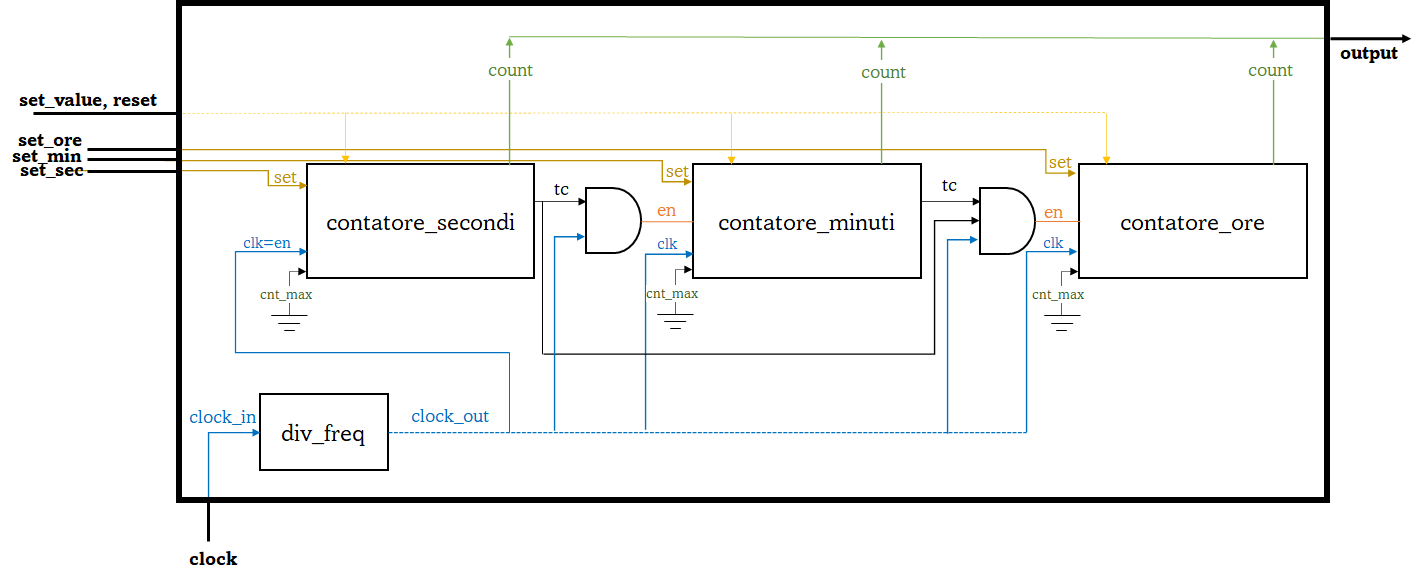
\includegraphics[width=17cm]{immagini/esercizio5/schema_5.1.png}
    \caption{Schema Cronometro}
\end{figure}

\paragraph{Contatore programmabile}
I primi tre contatori sono stati implementati a partire dallo stesso codice, tramite una \textit{entity contatore} realizzata con il costrutto \textit{generic}, al quale viene passato il valore \textit{n} che rappresenta il numero di bit necessari per effettuare il conteggio. 
Il contatore ha i seguenti input e output:
\begin{itemize}
\item \textit{cntmax}: serve per memorizzare il valore massimo del conteggio.
\item \textit{setvalue}: serve per memorizzare il valore da settare
\item \textit{clk}: segnale di clock
\item \textit{rst}: segnale di reset
\item \textit{set}: dà l’abilitazione al set al valore passato in setvalue
\item \textit{tc}: viene alzato quando si è arrivati al conteggio massimo
\item \textit{count}: valore  in uscita del conteggio corrente
\item \textit{en}: il segnale che proviene o dal clock diviso o da un altro contatore, e scandisce il momento in cui contare secondi, minuti o ore.
\end{itemize}
Il componente è stato realizzato con un unico \textit{process}, sensibile solo al \textit{clock} sul fronte di discesa, al cui interno ci sono una serie di costrutti di selezione in cascata. Inizialmente viene testata la condizione per il \textit{reset} sincrono, poi si controlla il valore di \textit{set} e nel caso è alto viene scritto nel registro il valore in input. Successivamente, se il valore di \textit{enable} è alto, si procede all'incremento del contatore,  e se si è raggiunto il valore massimo si riporta a zero e si alza l'uscita \textit{tc}. È di particolare importanza la scelta di utilizzare sia il \textit{clock} che il segnale \textit{enable}: tecnicamente si sarebbe potuto utilizzare solo il segnale di \textit{enable}, al posto del \textit{clock} normale, per abilitare i contatori in cascata (minuti e ore) , ma questo comporta che i \textit{process} si attivino ogni minuto o ogni ora. In questo modo non si sarebbe potuto  effettuare un \textit{reset} sincrono, a meno di aspettare un tempo eccessivo. L'ipotesi di usare invece un \textit{reset} asincrono è stata scartata in quanto creerebbe delle problematiche di accuratezza sull'orario misurato: se arrivasse il \textit{reset} asincrono poco prima di un nuovo \textit{clock} il secondo iniziale sarebbe contato molto prima del dovuto, come mostrato in figura.

\begin{figure}[H]
    \centering
    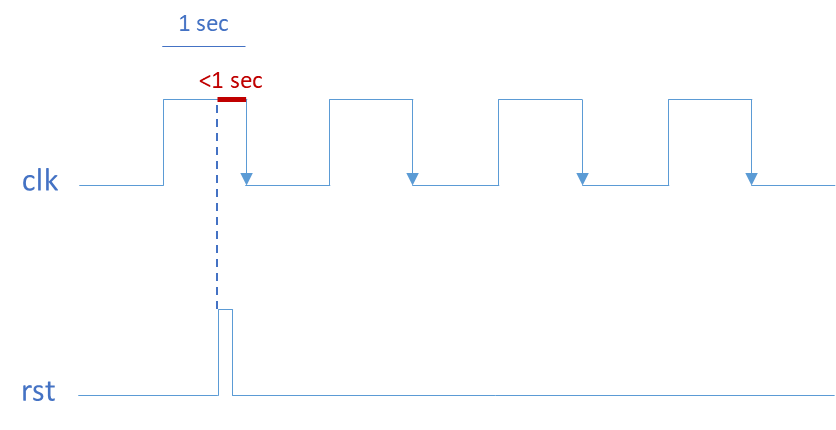
\includegraphics[width=17cm]{immagini/esercizio5/errore_reset.png}
    \caption{Reset Asincrono Errato}
\end{figure}

Di seguito il codice per l'implementazione di un contatore programmabile:
\begin{lstlisting} [language=VHDL, caption= Contatore programmabile]
library IEEE;
use IEEE.std_logic_1164.all;
use IEEE.numeric_std.all;

entity contatore is
    generic (
        n: positive
    );
    port (
        cnt_max, set_value: in std_logic_vector(n-1 downto 0);
        clk, rst, set, en: in std_logic;
        tc: out std_logic;
        count: out std_logic_vector(n-1 downto 0)
    );
end entity contatore;

architecture rtl of contatore is

begin
    proc_name: process(clk)
        variable current: unsigned(n-1 downto 0) := (others => '0');
    begin
        if falling_edge (clk) then
            if rst = '1' then
                current := (others => '0');
                tc <= '0';

            elsif set = '1' then
                current := unsigned(set_value);

            elsif en = '1' and  (unsigned(cnt_max) - 1 = current) then
                current := (others => '0');

            elsif en = '1' then
                current := current +1;
            end if;

            if(unsigned(cnt_max) - 1 = current ) then
                tc <= '1';
            else 
                tc <= '0';
            end if;
        end if;
        
        count <= std_logic_vector(current);
        
    end process proc_name;
end architecture rtl;
\end{lstlisting}

\paragraph{Divisore di frequenza}
Il divisore di frequenza è un componente necessario e serve per generare un impulso a frequenza inferiore rispetto a quella del \textit{clock} in entrata, che nel nostro caso è proprio il \textit{clock} a 100MHz della scheda.
Anche questo componente utilizza il costrutto \textit{generic} per poter essere \textit{istanziato} con diverse impostazioni. In particolare, è possibile specificare la frequenza in entrata e quella in uscita. Dopo aver inserito questi due valori viene calcolato il massimo conteggio da effettuare, in modo da alzare l'uscita una volta raggiunto il valore \textit{cnt\_max-1}. In questo caso la frequenza di uscita è stata scelta a 1Hz in modo da avere un impulso al secondo.

Il componente è stato realizzato mediante il seguente codice:
\begin{lstlisting} [language=VHDL, caption= Divisore di frequenza]
library IEEE;
use IEEE.STD_LOGIC_1164.ALL;
 
entity clock_divider is
     generic(
          clock_frequency_in : integer := 100000000;--100MHz
          clock_frequency_out : integer := 1 --1 Hz
         );
    Port ( clock_in : in  STD_LOGIC;
           reset : in STD_LOGIC;
           clock_out : out  STD_LOGIC);
end clock_divider;
 
architecture Behavioral of clock_divider is
 
signal clockfx: std_logic := '0';
constant count_max_value: integer := (clock_frequency_in/clock_frequency_out)-1;
begin
  clock_out <= clockfx;
 
    count_for_division: process(clock_in)
    variable counter: integer range 0 to count_max_value := 0;
    begin
       if rising_edge(clock_in)  then
       
        if reset = '1' then
             counter := 0;
             clockfx <= '0';
        else
          if counter = count_max_value then
              clockfx <=  '1';
              counter := 0;
           else
              clockfx <=  '0';
              counter := counter + 1;
          end if;
        end if;
       end if;
    end process;
end Behavioral;
\end{lstlisting}

\paragraph{Cronometro}
I singoli componenti analizzati fin ora sono stati collegati tra loro per realizzare il cronometro. Vengono creati tre contatori(due contano fino a 60 e uno fino a 24) e un divisore di frequenza. L'uscita del divisore (un \textit{clock} a 1 secondo) entra come \textit{enable} nel contatore dei secondi, mentre per i contatori successivi viene effettuata una \textit{AND} tra questo segnale e i segnali di uscita \textit{tc} per i minuti e le ore. In questo modo i segnali di abilitazione per scandire i minuti e le ore avranno la giusta durata, e non sarà possibile contare più volte con lo stesso fronte del segnale.
L'output totale viene calcolato concatenando le uscite dei singoli contatori in ordine.

\begin{lstlisting} [language=VHDL, caption=Cronometro]
library IEEE;
use IEEE.STD_LOGIC_1164.ALL;

entity cronometro is
    Port (
        set_value: in std_logic_vector (5 downto 0 );
        set_sec,set_min,set_ore: in std_logic;
        reset: in std_logic;
        clock: in std_logic;
        output: out std_logic_vector (16 downto 0 )
    );
end cronometro;

architecture Structural of cronometro is

    component contatore is
        generic (
            n: positive
        );
        Port (
            cnt_max, set_value: in std_logic_vector(n-1 downto 0);
            clk, rst, set, en: in std_logic;
            tc: out std_logic;
            count: out std_logic_vector(n-1 downto 0)
        );
    end component;

    component clock_divider is
        generic(
            clock_frequency_in : integer := 100000000;--100MHz
            clock_frequency_out : integer := 10000000 --10 MHz
        );
        Port ( clock_in : in  STD_LOGIC;
             reset : in STD_LOGIC;
             clock_out : out  STD_LOGIC);
    end component;

    signal s_clk:std_logic;
    signal s_tc1,s_tc2:std_logic;
    signal s_conteggio_sec,s_conteggio_min:std_logic_vector(5 downto 0);
    signal s_conteggio_ore:std_logic_vector(4 downto 0);
    signal s_count_60:std_logic_vector(5 downto 0):="111100";
    signal s_count_24:std_logic_vector(4 downto 0):="11000";

begin

    contatore_sec: contatore
        generic map (
            n=>6
        )
        port map(
            cnt_max=>s_count_60,
            set_value=>set_value,
            clk=>clock,
            en=>s_clk,
            rst=>reset,
            set=>set_sec,
            tc=>s_tc1,
            count=>s_conteggio_sec
        );

    contatore_min: contatore
        generic map (
            n=>6
        )
        port map(
            cnt_max=>s_count_60,
            set_value=>set_value,
            en=>s_clk and s_tc1 ,
            clk=>clock,
            rst=>reset,
            set=>set_min,
            tc=>s_tc2 ,
            count=>s_conteggio_min
        );

    contatore_ore: contatore
        generic map (
            n=>5
        )
        port map(
            cnt_max=>s_count_24,
            set_value=>set_value(4 downto 0),
            en=> s_tc1 and s_clk and s_tc2,
            clk=>clock,
            rst=>reset,
            set=>set_ore,
            count=>s_conteggio_ore
        );
    divisore: clock_divider
        generic map(
            clock_frequency_in => 100000000 ,
            clock_frequency_out=> 1
        )
        port map(
            clock_in=>clock,
            reset=>reset,
            clock_out=>s_clk
        );

    output<=s_conteggio_sec & s_conteggio_min & s_conteggio_ore;

end Structural;
\end{lstlisting}

\subsection{Testing}
\paragraph{Testbench}
Data la complessità dell'architettura sono stati effettuati due testbench separati. Uno per il contatore programmabile e uno per il cronometro completo. 
Nel primo sono state testate le funzionalità di scrittura sul registro e le possibili risposte ai segnali di reset ed enable e non sono state riscontrate anomalie.

Il secondo testbench resetta il dispositivo e ne osserva il comportamento, per verificare se vengono scanditi correttamente i secondi, i minuti e le ore. È da notare che durante le fasi di test il divisore di frequenza è stato programmato con un output molto più alto di 1Hz, in modo da controllare più velocemente i risultati.

I casi di test sono stati realizzati mediante i seguenti codici:
\begin{lstlisting} [language=VHDL, caption=Testbench contatore]
library IEEE;
use IEEE.std_logic_1164.all;
use IEEE.numeric_std.all;

entity cont_tb is
end entity cont_tb;

architecture test of cont_tb is
    component contatore is
        generic (
            n: positive
        );
        port (
            cnt_max, set_value: in std_logic_vector(n-1 downto 0);
            clk, rst, set: in std_logic;
            tc: out std_logic;
            count: out std_logic_vector(n-1 downto 0)
        );
    end component;

    signal tb_in, tb_count, tb_set_value: std_logic_vector(5 downto 0) := (others => '0');
    signal tb_set, tb_ck, tb_rst, tb_tc: std_logic := '0';
    constant clk_period: time := 5 ns;
    
begin
    dut: contatore
    generic map(n => 6)
    port map (
        tb_in, 
        tb_set_value, 
        tb_ck, 
        tb_rst, 
        tb_set, 
        tb_tc, 
        tb_count
    );

    ns_counter: process 
    begin
        tb_in <= "111100";
        tb_rst <= '1';
        wait for 20 ns;
        tb_rst <= '0';
        wait for clk_period * 2;
        assert (tb_count = "000010") report "expected 2" severity failure;
        wait for clk_period * 5;
        assert (tb_count = "000111") report "expected 7" severity failure;
        wait;
    end process ns_counter;
    clock: process
    begin
        for i in 0 to 99
        loop
            tb_ck <= '1';
            wait for clk_period/2;
            tb_ck <= '0';
            wait for clk_period/2;
        end loop;
        wait;
    end process clock;
    
end architecture test;


\end{lstlisting}


\begin{lstlisting} [language=VHDL, caption= Testbench cronometro]
library IEEE;
use IEEE.STD_LOGIC_1164.ALL;

entity cronometro_tb is
end cronometro_tb;

architecture Behavioral of cronometro_tb is

component cronometro is
    Port (

        set_value: in std_logic_vector (5 downto 0 );
        set_sec,set_min,set_ore: in std_logic;
        reset: in std_logic;
        clock: in std_logic;
        output: out std_logic_vector (16 downto 0 )
    );
end component cronometro;

signal s_set_sec, s_set_min, s_set_ore, s_reset, s_clock: std_logic  := '0';
signal s_output: std_logic_vector(16 downto 0 ) :=  (others => '0');
signal s_set_value: std_logic_vector(5 downto 0 ) :=  (others => '0');
constant clk_period: time := 10 ps;

begin

   dut: cronometro
    port map (
        set_value => s_set_value,
        set_sec=> s_set_sec,
        set_min=> s_set_min,
        set_ore=> s_set_ore,
        reset=> s_reset,
        clock => s_clock,
        output => s_output
    );  
      
    tb: process
    begin
            wait for 100ns;
            s_reset <= '1';
            wait for 10ns;
            s_reset <= '0';
            
            wait for 1000ns;
            
            wait;
    end process tb;
    
    clock: process
    begin
            s_clock <= '1';
            wait for clk_period/2;
            s_clock <= '0';
            wait for clk_period/2;
    end process clock;

end Behavioral;


\end{lstlisting}

\section{Sintesi su scheda}
\paragraph{Traccia} Sintetizzare ed implementare su board il componente sviluppato al punto precedente, utilizzando i display a 7 segmenti per la visualizzazione dell’orario (o una combinazione di display e led nel caso in cui i display a disposizione siano in numero inferiore a quello necessario), gli switch per l’immissione dell’orario iniziale e due bottoni, uno per il set dell’orario e uno per il reset. Si utilizzi una codifica a scelta dello studente per la visualizzazione dell’orario sui display (esadecimale o decimale).


\subsection{Implementazione}
Come negli esercizi precedenti sono stati utilizzati dei button debouncer per gestire i segnali di input dei bottoni. In particolare sono stati aggiunti tre pulsanti, uno per il set dei secondi, uno per i minuti e uno per le ore. Per impostare il valore da scrivere sono stati scelti i primi sei switch della board, ma nel caso del set delle ore l'ultimo switch viene ovviamente ignorato. 
Per poter visualizzare l'output sullo schermo a led della scheda è stato utilizzato il componente \textit{seven\_segment\_array}, fornitoci durante il corso. Sono però state effettuate delle modifiche in modo da ottimizzare la visualizzazione delle cifre:
Innanzitutto sono stati spenti 2 schermi in modo da creare dello spazio tra la visualizzazione dei secondi, minuti e ore. Di base poi l'output del cronometro veniva letto come un unico numero a 17 bit, quindi anche se tecnicamente corretto l'orario non era facilmente comprensibile per l'utente. È stato modificato quindi il componente \textit{cathodes\_input\_manager}, in modo da separare i bit dei diversi contatori, assegnando 2 cifre a ognuno. Dato che è stata utilizzata una rappresentazione esadecimale a ogni cifra devono essere assegnati 4 bit, ma le uscite dei contatori, divise in due parti, non sono sufficienti, per cui sono stati aggiunti due bit nulli in testa ad alcuni schermi.
Sono stati infine mappati i segnali opportuni sul file dei \textit{constraint}.

Di seguito è mostrato il codice relativo al componente generale che ingloba gli altri:
\begin{lstlisting} [language=VHDL, caption= Testbench cronometro]
library IEEE;
use IEEE.STD_LOGIC_1164.ALL;

entity top is
  Port ( 
        set_value: in std_logic_vector (5 downto 0 );
        set_sec,set_min,set_ore: in std_logic;
        reset: in std_logic;
        clock: in std_logic;
        anodes : out  STD_LOGIC_VECTOR (7 downto 0);
        cathodes : out  STD_LOGIC_VECTOR (7 downto 0);
	clock_out: out std_logic;
	output: out std_logic_vector (5 downto 0)
  );
end top;

architecture Structural of top is

component cronometro is
    Port (
        set_value: in std_logic_vector (5 downto 0 );
        set_sec,set_min,set_ore: in std_logic;
        reset: in std_logic;
        clock: in std_logic;
        clock_out:out std_logic ;
        out_sec:out std_logic_vector (5 downto 0);
        output: out std_logic_vector (16 downto 0 )
    );
end component cronometro;

component ButtonDebouncer 
    generic (                       
        CLK_period: integer := 10;
        btn_noise_time: integer := 5000000
    );
    port ( RST : in STD_LOGIC;
           CLK : in STD_LOGIC;
           BTN : in STD_LOGIC;
           CLEARED_BTN : out STD_LOGIC);
end component;
  
component display_seven_segments
    generic(
        clock_frequency_in : integer := 50000000; 
        clock_frequency_out : integer := 5000000
    );
    port(
        clock : in  STD_LOGIC;
        reset : in  STD_LOGIC;
        value32_in : in  STD_LOGIC_VECTOR (31 downto 0);
        enable : in  STD_LOGIC_VECTOR (7 downto 0);
        dots : in  STD_LOGIC_VECTOR (7 downto 0);
        anodes : out  STD_LOGIC_VECTOR (7 downto 0);
        cathodes : out  STD_LOGIC_VECTOR (7 downto 0)
    );
end component;

signal set_sec_debouncer, set_min_debouncer, set_ore_debouncer : std_logic;
signal value_temp : std_logic_vector(31 downto 0);
signal s_clock_out, s_sus: std_logic:='0';

begin

  debouncer1: ButtonDebouncer GENERIC MAP( 
        CLK_period => 10,  -- periodo del clock della board pari a 10ns
        btn_noise_time => 5000000 -- assumo un periodo di oscillazione di 5 millisec
   )
   PORT MAP ( RST => reset,
           CLK => clock , 
           BTN => set_sec,
           CLEARED_BTN => set_sec_debouncer                                                            
  );

  debouncer2: ButtonDebouncer GENERIC MAP( 
        CLK_period => 10,  -- periodo del clock della board pari a 10ns
        btn_noise_time => 5000000 -- assumo un periodo di oscillazione di 5 millisec
  )
   PORT MAP ( RST => reset,
           CLK => clock, 
           BTN => set_min,
           CLEARED_BTN => set_min_debouncer
  );

  debouncer3: ButtonDebouncer GENERIC MAP( 
        CLK_period => 10,  
        btn_noise_time => 5000000
  )
   PORT MAP ( RST => reset,
           CLK => clock, 
           BTN => set_ore,
           CLEARED_BTN => set_ore_debouncer                                     
  );

 seven_segment_array: display_seven_segments GENERIC MAP(
	clock_frequency_in => 100000000,
	clock_frequency_out => 500
	)
     PORT MAP(
	clock => clock,
	reset => reset,
	value32_in => value_temp,
	enable => "11011011", --stabilisco che tutti i display siano accesi 
	dots => "00000000",  --stabilisco che tutti i punti siano spenti
	anodes => anodes,
	cathodes => cathodes
 );

cron: cronometro port map(
     set_value=>set_value,
     set_sec=> set_sec_debouncer ,
     set_min=> set_min_debouncer ,
     set_ore=> set_ore_debouncer ,
     reset=>reset,
     clock=>clock,
     clock_out=>s_clock_out ,
     out_sec=>output,
     output =>value_temp(16 downto 0)
);

 process (s_clock_out)
   begin
     if rising_edge (s_clock_out ) then
         s_sus <= not s_sus;
     end if;
 end process;
    clock_out <= s_sus ;
   
end Structural;
\end{lstlisting}

\section{Cronometro con intertempo}

\subsection{Architettura}
\paragraph{Traccia} 
Estendere il componente sviluppato ai punti precedenti in modo che sia in grado di acquisire e memorizzare internamente fino ad un numero N di intertempi in corrispondenza di un ingresso di stop. Opzionalmente, il componente può prevedere una modalità di visualizzazione in cui, alla  pressione di un bottone, vengano visualizzati sui display gli intertempi memorizzati (uno per ogni pressione).

\subsection{Implementazione}
Per estendere le funzionalità del sistema esaminato nelle sezioni precedenti, è stato inserito uno shift register in modo da memorizzare, in presenza di un segnale \textit{stop}, gli intertempi in uscita dal cronometro. È stato istanziato quindi un registro a scorrimento basato su quello visto precedentemente, con quattro registri da 17 bit, ma con la possibilità di scegliere tra due modalità:
\begin{itemize}
\item In modalità 0, o scrittura , si comporta come un normale shift register, che inserisce in testa il nuovo dato. 
\item In modalità 1, o lettura, invece di scrivere nella primo registro, si limita a far scorrere ciclicamente i dati, in modo che sia possibile consultarli uno per uno senza il rischio di perderli. 
\end{itemize}
L'architettura totale è visibile nel seguente schema:

\begin{figure}[H]
    \centering
    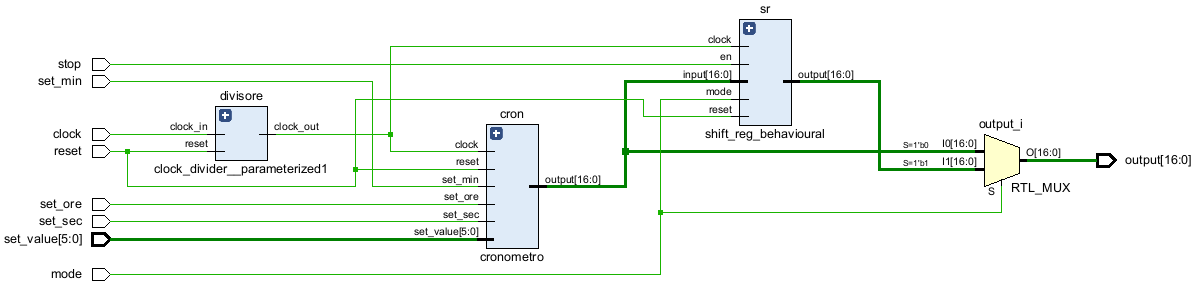
\includegraphics[width=17cm]{immagini/esercizio5/schema_5.3.png}
    \caption{Schema Cronometro con Intertempo}
\end{figure}


È stato necessario però gestire la visualizzazione dell'output del sistema complessivo, in cui si deve scegliere se mostrare l'uscita del cronometro (tempo real-time) o quella del registro a scorrimento (intertempi). Per farlo è stata aggiunta un'assegnazione combinatoria, che cambia l'output a seconda della modalità:

Di seguito è mostrato il codice relativo al componente che ingloba gli altri e allo shift register modificato.

\begin{lstlisting} [language=VHDL, caption= Top]
library IEEE;
use IEEE.STD_LOGIC_1164.ALL;

entity top is
    Port (
        set_value: in std_logic_vector (5 downto 0);
        set_sec,set_min,set_ore,mode,stop: in std_logic;
        reset: in std_logic;
        clock: in std_logic;
        output: out std_logic_vector (16 downto 0)
    );
end top;

architecture Structural of top is

    component shift_reg_behavioural is
        Port (
            input: in std_logic_vector (16 downto 0);
            clock,en: in std_logic ;
            reset,mode: in std_logic ;--mode 0: scrittura, mode 1: lettura
            output: out std_logic_vector (16 downto 0)
        );
    end component shift_reg_behavioural;

    component  cronometro is
        Port (
            set_value: in std_logic_vector (5 downto 0);
            set_sec,set_min,set_ore: in std_logic;
            reset: in std_logic;
            clock: in std_logic;
            output: out std_logic_vector (16 downto 0)
        );
    end component cronometro;
    component clock_divider is
        generic(
            clock_frequency_in : integer := 100000000;--100MHz
            clock_frequency_out : integer := 10000000 --10 MHz
        );
        Port ( clock_in : in  STD_LOGIC;
             reset : in STD_LOGIC;
             clock_out : out  STD_LOGIC);
    end component;

    signal cron_out,shift_out: std_logic_vector (16 downto 0);
    signal s_clk:std_logic ;

begin

    cron: cronometro 
        port map(
            set_value=> set_value,
            set_sec=>set_sec,
            set_min=>set_min,
            set_ore=>set_ore,
            reset=>reset,
            clock=>s_clk,
            output =>cron_out
        );

    sr: shift_reg_behavioural 
        port map(
            input=>cron_out,
            en=> stop,
            mode=> mode,
            reset=>reset,
            clock=>s_clk,
            output=>shift_out
        );


    divisore: clock_divider
        port map(
            clock_in=>clock,
            reset=>reset,
            clock_out=>s_clk
        );
    with mode select output <=
        cron_out  when '0',
        shift_out when '1',
        cron_out when others;

end Structural;


\end{lstlisting}


\begin{lstlisting} [language=VHDL, caption= Shift Register]
library IEEE;
use IEEE.STD_LOGIC_1164.ALL;

entity shift_reg_behavioural is
    Port (
        input: in std_logic_vector (16 downto 0);
        clock,en: in std_logic ;
        reset,mode: in std_logic ; --mode 0 : scrittura, mode 1: lettura
        output: out std_logic_vector (16 downto 0)
    );
end shift_reg_behavioural;

architecture Behavioral of shift_reg_behavioural is

   signal s1,s2,s3,s4: std_logic_vector (16 downto 0):="00000000000000000";

begin

    process (clock)
    begin
        if (falling_edge (clock)) then
        
            if ( reset='1') then
                s1<="00000000000000000";
                s2<="00000000000000000";
                s3<="00000000000000000";
                s4<="00000000000000000";
            
            elsif (mode='0' and en='1') then
                s1<=input;
                s2<=s1;
                s3<=s2;
                s4<=s3;
                
            elsif (mode ='1'and en='1') then
                s1<=s4;
                s2<=s1;
                s3<=s2;
                s4<=s3;
            end if;
        end if;
    end process;

    output<= s4;

end Behavioral;
\end{lstlisting}


\subsection{Testing}
È stato effettuato unicamente il test dell'unità top, essendo stati già precedentemente testati tutti gli altri componenti. In primo luogo, è stato effettuato il reset della macchina e successivamente sono stati mandati i segnali di stop per memorizzare gli intertempi. In particolare, sono stati memorizzati 4 intertempi e successivamente sono stati visionati in maniera circolare per 3 volte.

\begin{lstlisting} [language=VHDL, caption= Shift Register]
library IEEE;
use IEEE.STD_LOGIC_1164.ALL;

entity top_tb is
end top_tb;

architecture Behavioral of top_tb is

component top is
Port (
        set_value: in std_logic_vector (5 downto 0 );
        set_sec,set_min,set_ore,mode,stop: in std_logic;
        reset: in std_logic;
        clock: in std_logic;
        output: out std_logic_vector (16 downto 0 )
    );
end component top;

signal s_set_sec, s_set_min, s_set_ore, s_reset, s_clock, s_mode, s_stop: std_logic  := '0';
signal s_output: std_logic_vector(16 downto 0 ) :=  (others => '0');
signal s_set_value: std_logic_vector(5 downto 0 ) :=  (others => '0');
constant clk_period: time := 1 ns;

begin
   dut: top
    port map (
        set_value => s_set_value,
        set_sec=> s_set_sec,
        set_min=> s_set_min,
        set_ore=> s_set_ore,
        reset=> s_reset,
        clock => s_clock,
        output => s_output,
        mode=> s_mode,
        stop=>s_stop
    );
    
    tb: process
    begin
            wait for 100ns;
            s_reset <= '1';
            wait for 10ns;
            s_reset <= '0';
            
            wait for 50ns;
            s_stop<='1';
            wait for 10*clk_period;
            s_stop<='0';
            wait for 10ns;
            s_stop<='1';
            wait for 10*clk_period;
            s_stop<='0';
            wait for 30ns;
            s_stop<='1';
            wait for 10*clk_period;
            s_stop<='0';
            wait for 10ns;
            s_stop<='1';
            wait for 10*clk_period;
            s_stop<='0';
            
            wait for 50ns;
            s_mode<='1';
            wait for 10*clk_period;
            s_stop<='1';
            wait for 10*clk_period;
            s_stop<='0';
            wait for 10*clk_period;
            s_stop<='1';
            wait for 10*clk_period;
            s_stop<='0';
            wait for 10*clk_period;
            s_stop<='1';
            wait for 10*clk_period;
            s_stop<='0';
            wait for clk_period ;
            wait;
    end process tb;
    
    clock: process
    begin
        s_clock <= '1';
        wait for clk_period/2;
        s_clock <= '0';
        wait for clk_period/2;
    end process clock;
end Behavioral;
\end{lstlisting}
\chapter{Sistema di testing}

\section{Sistema di testing}
\paragraph{Traccia}
Progettare, implementare in VHDL e verificare mediante simulazione un sistema in grado di testare in maniera automatica una macchina combinatoria M avente 4 ingressi e 3 uscite binarie sottoponendole N ingressi diversi (si considerino una macchina M e un numero di input N a scelta dello studente). 
Gli N valori di input per il test devono essere letti da una ROM, in cui essi sono precaricati, in corrispondenza di un segnale read. Le N uscite fornite della macchina in corrispondenza di ciascuno degli input devono essere memorizzate in una memoria interna, che deve poter essere svuotata in qualsiasi momento in presenza di un segnale di reset.


\subsection{Architettura}
L'architettura della soluzione è illustrata in Figura \ref{fig:Architettura sistema di testing} ed è composta dai seguenti componenti:
\begin{itemize}
    \item \textit{ROM}: memoria di sola lettura che contiene gli ingressi da inviare alla macchina combinatoria;
    \item \textit{Macchina combinatoria}: macchina che riceve un ingresso a 4 bit e offre un uscita a 3 bit;
    \item \textit{Memoria}: si occupa di memorizzare il risultato delle operazioni in uscita dalla macchina combinatoria;
    \item \textit{Rete di controllo}: si occupa di gestire la tempificazione della macchina fornendo i segnali di scrittura e indirizzo alle memorie;
\end{itemize}

\begin{figure}[H]
    \centering
    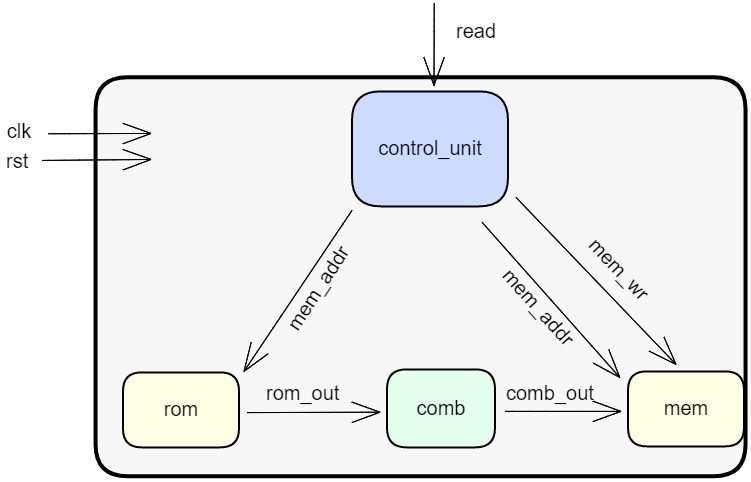
\includegraphics[width=15cm]{immagini/esercizio6/schema_6.1.png}
    \caption{Architettura sistema di testing}
    \label{fig:Architettura sistema di testing}
\end{figure}

\paragraph{Rete di controllo}
La rete di controllo è stata implementata attraverso l'automa a stati finiti illustrato in Figura \ref{fig:fsm_6}. Il sistema si predispone alla memorizzazione del risultato della macchina combinatoria ponendo \textit{mem\_wr=1} nello stato \textit{load} e poi si blocca in attesa del segnale di \textit{read} nello stato \textit{wait\_read}. Infine, lo stato \textit{ctrl} serve a rendere consistente l'incremento del segnale di indirizzo \textit{mem\_addr}.

\begin{figure}[H]
    \centering
    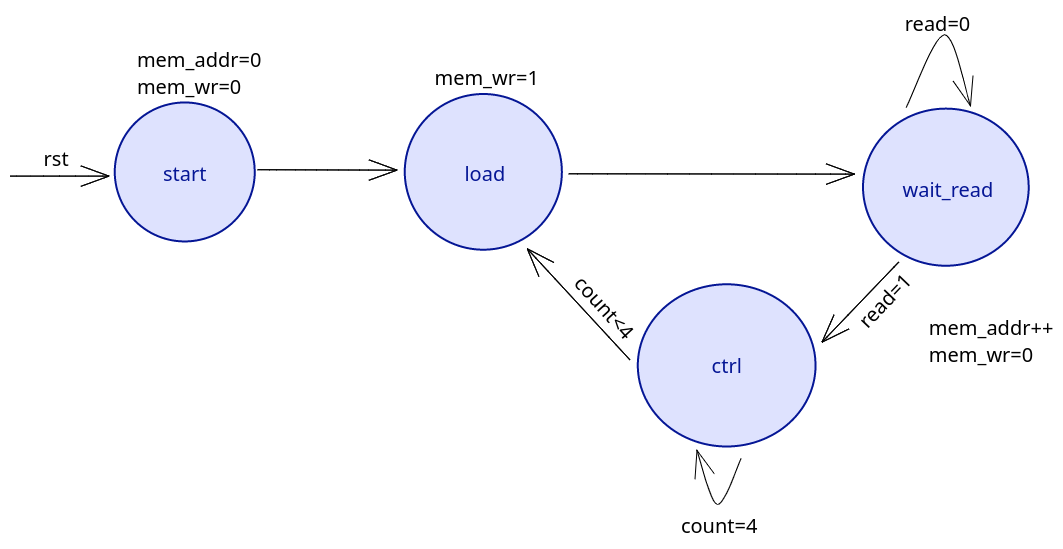
\includegraphics[width=16cm]{immagini/esercizio6/automa_6.1.png}
    \caption{Automa a stati finiti}
    \label{fig:fsm_6}
\end{figure}

Nel listato \ref{fsm_6} è mostrata l'implementazione dell'automa in Figura \ref{fig:fsm_6}.

\begin{lstlisting} [language=VHDL,label=fsm_6, caption=Implelemtazione automa a stati finiti] 
library IEEE;
use IEEE.STD_LOGIC_1164.ALL;
use ieee.numeric_std.all ;

entity rete_di_controllo is
    Port (
        clk,reset,read: in std_logic ;
        addr: out std_logic_vector (1 downto 0);
        write: out std_logic

    );
end rete_di_controllo;

architecture Behavioral of rete_di_controllo is

    type state is (
        START,
        LOAD,
        WAIT_READ,
        CTRL
    );
    signal current_state : state:= START;
    signal next_state : state;
    signal s_addr: std_logic_vector (1 downto 0);
begin
    comb: process(current_state,read)
    variable count: integer:=0;

    begin
        case current_state is
        
            when START =>
                s_addr<="00";
                write<='0';
                count:=0;
                next_state<= LOAD ;
                
            when LOAD  =>
                next_state<= WAIT_READ ;
                write<='1';
 
            when WAIT_READ  =>
                if (read='1') then
                    next_state<= CTRL  ;
                    write<='0';
                    s_addr <= std_logic_vector((unsigned(s_addr) + 1));
                    count:=count+1;
                else
                    next_state<= WAIT_READ ;
                end if;

            when CTRL =>
                if (count=4)then
                   next_state<= CTRL ;
                else 
                   next_state<= LOAD;
                end if;

            when others =>
                next_state<= START;
        end case;
    end process;
    
addr<=s_addr ;

    seq: process(clk)
    begin
        if rising_edge(clk) then
            if reset='1' then
                current_state<=START;
            else
                current_state<=next_state;
            end if;
        end if;
    end process seq;

end Behavioral;

\end{lstlisting}


\paragraph{Rom}
La rom è stata implementata con un processo ed è rappresentata da un \textit{array} di vettori da $3$ bit. In particolare, è stata scelta un'implementazione \textit{single port} con lettura asincrona. Nel listato \ref{rom_6} è mostrata l'implementazione della rom.

\begin{lstlisting}[language=VHDL,label=rom_6, caption=Implelemtazione automa a stati finiti]
library ieee;
use ieee.std_logic_1164.all;
use ieee.numeric_std.all;

entity rom is
port(
    clk, read : in std_logic; 
    addr : in std_logic_vector(1 downto 0);
    data : out std_logic_vector(3 downto 0)
    );
end rom;

architecture behavioral of rom is 
type rom_type is array (0 to 3) of std_logic_vector(3 downto 0);
signal ROM : rom_type := (
    "0001", 
    "0110", 
    "1011", 
    "1111"
);

begin

process(clk)
  begin
    if rising_edge(clk) then
          data <= rom(to_integer(unsigned(addr)));
    end if;
end process;
end behavioral;
\end{lstlisting}

\paragraph{Macchina combinatoria}
La macchina combinatoria scelta effettua un'operazione molto semplice che trasforma un ingresso a $4$ bit in uscita a $3$ bit. In particolare, dato un ingresso $X=X_3X_2X_1X_0$, l'uscita $Y$ si ottiene nel seguente modo:
\begin{equation*}
    Y = (X_3\;AND\;X_2)\;\&X_1\;\&\;X_0
\end{equation*}
dove con il simbolo $\&$ si indica l'operazione di concatenamento.
 
\begin{lstlisting} [language=VHDL, caption=Macchina combinatoria]
library IEEE;
use IEEE.STD_LOGIC_1164.ALL;

entity macchina_combinatoria is
    port(
        input: in std_logic_vector(3 downto 0);
        output: out std_logic_vector( 2 downto 0)
    );
end macchina_combinatoria;

architecture behavioral of macchina_combinatoria is

begin
    output <= (input(3)and input(2)) & input(1) & input(0);
end behavioral;

\end{lstlisting}

\paragraph{Memoria}
In maniera simile alla ROM, la memoria è implementata con un approccio comportamentale. In particolare, è stata scelta una memoria \textit{single-port} con lettura asincrona effettua la scrittura in corrispondenza del segnale di ingresso \textit{write}. Nel listato \ref{memoria}, è riportata l'implementazione della memoria.
\begin{lstlisting} [language=VHDL, label=memoria, caption=Implementazione memoria]
library ieee;
use ieee.std_logic_1164.all;
use ieee.std_logic_unsigned.all;

entity memoria is
port(
    clk, read, write, reset : in std_logic; 
    addr : in std_logic_vector(1 downto 0);
    input : in std_logic_vector(2 downto 0);
    output : out std_logic_vector(2 downto 0)
    );
end memoria;

architecture behavioral of memoria is 
type memoria_type is array (0 to 3) of std_logic_vector(2 downto 0);
signal MEM : memoria_type := (
    "000", 
    "000", 
    "000", 
    "000"
);

begin
    process(clk)
      begin
        if rising_edge(clk) then
            if reset = '1' then
                 for i in 0 to 3 loop 
                     MEM(i) <= "000";
                 end loop;
            elsif write = '1' then
                MEM(conv_integer(addr)) <= input;        
            end if;
        end if;
        output<=MEM(conv_integer(addr));   
    end process;
end behavioral;
\end{lstlisting}

\paragraph{Sistema complessivo} Il sistema complessivo è stato assemblato a partire dai componenti descritti in precedenza e collegati in maniera opportuna. In particolare, attraverso il segnale \textit{mem\_addr} la rete di controllo si interfaccia con la ROM e la memoria. Quest'ultima riceve anche il segnale di \textit{write} per la scrittura. Inoltre, attraverso il segnale \textit{s\_data}, l'uscita della ROM è collegata in ingresso alla macchina combinatoria; mentre la sua uscita è collegata in ingresso alla memoria mediante il segnale \textit{s\_output}. Nel listato \ref{sis_6_1}, è mostrato il sistema complessivo.

\begin{lstlisting} [language=VHDL, label=sis_6_1, caption=Sistema complessivo]
library IEEE;
use IEEE.STD_LOGIC_1164.ALL;

entity test_automatico is
  Port ( 
    clk, reset, read: in std_logic;
    out_123: out std_logic_vector(2 downto 0)
  );
end test_automatico;

architecture structural of test_automatico is

component macchina_combinatoria is
    port(
        input: in std_logic_vector(3 downto 0);
        output: out std_logic_vector( 2 downto 0)
    );
end component macchina_combinatoria;

component memoria is
port(
    clk, read, write, reset : in std_logic; 
    addr : in std_logic_vector(1 downto 0);
    input : in std_logic_vector(2 downto 0);
    output : out std_logic_vector(2 downto 0)
    );
end component memoria;

component rom is
port(
    clk, read : in std_logic; 
    addr : in std_logic_vector(1 downto 0);
    data : out std_logic_vector(3 downto 0)
    );
end component rom;

component rete_di_controllo is
    port(
    clk,reset,read: in std_logic;
    write: out std_logic;
    addr: out std_logic_vector(1 downto 0) 
);
end component rete_di_controllo;

signal s_write : std_logic := '0';
signal s_addr : std_logic_vector(1 downto 0) := "00";
signal s_data: std_logic_vector(3 downto 0) := "0000";
signal s_output: std_logic_vector(2 downto 0) := "000";
begin

MC: macchina_combinatoria port map(
      input=>s_data,
      output=>s_output
);

M: memoria port map (
    clk=>clk,
    read=>read,
    write=>s_write,
    addr=>s_addr,
    reset=>reset,
    input=>s_output,
    output=>out_123
);

R: rom port map (
 clk=>clk,
 read=>read,
 addr=>s_addr,
 data=>s_data
);

RC: rete_di_controllo port map(
    clk=>clk,
    read=>read,
    write=>s_write,
    reset=>reset,
    addr=>s_addr
);

end structural;
\end{lstlisting}

\subsection{Testing}
Il sistema è stato testato fornendo in ingresso 4 segnali di \textit{read} distinti. In uscita, come mostrato nella simulazione in Figura \ref{fig:sim_6.1}, ad ogni \textit{read}, l'uscita commuta correttamente con il risultato della macchina combinatoria. Il \textit{testbench} è riportato nel listato \ref{tb_sis_6.1}.

\begin{lstlisting} [language= VHDL, label=tb_sis_6.1, caption=Testbench sistema complessivo]
library IEEE;
use IEEE.STD_LOGIC_1164.ALL;

entity test_automatico_tb is
end test_automatico_tb;

architecture Behavioral of test_automatico_tb is

    component test_automatico is
        Port (
            clk, reset, read: in std_logic;
            out_123: out std_logic_vector(2 downto 0)
        );
    end component test_automatico;

    signal s_clk, s_reset, s_read : std_logic := '0';
    signal s_output:  std_logic_vector(2 downto 0):="000";
    constant clk_period: time := 10 ns;
begin

    uut: test_automatico port map(
            clk=>s_clk,
            reset=>s_reset,
            read=>s_read,
            out_123=>s_output
        );

    clock: process
    begin
        s_clk <= not s_clk;
        wait for clk_period/2;
    end process clock;

    sus: process
    begin
        wait for 100ns;
        s_reset <='1';
        wait for clk_period;
        s_reset <='0';
        wait for 5*clk_period;

        s_read <= '1';
        wait for clk_period;
        s_read <= '0';
        wait for 5*clk_period;

        s_read <= '1';
        wait for clk_period;
        s_read <= '0';
        wait for 5*clk_period;

        s_read <= '1';
        wait for clk_period;
        s_read <= '0';
        wait for 5*clk_period;

        s_read <= '1';
        wait for clk_period;
        s_read <= '0';
    wait;
    end process sus;
end Behavioral;


\end{lstlisting} 

\begin{figure}[H]
    \centering
    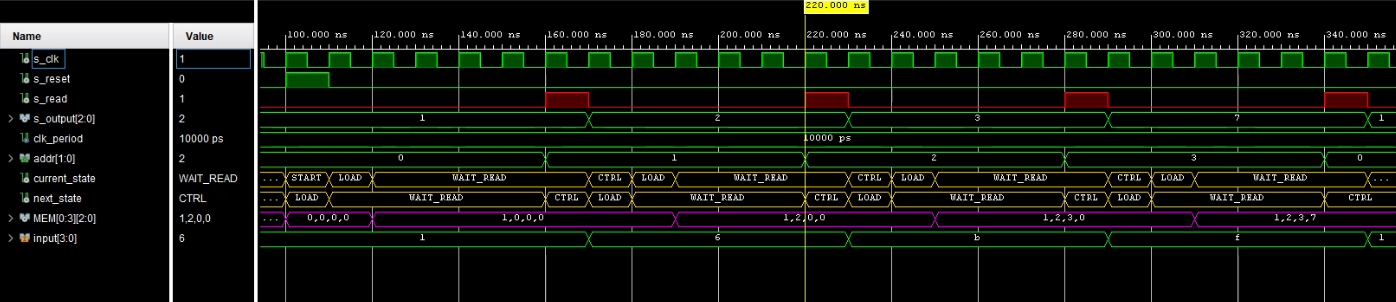
\includegraphics[width=15cm]{immagini/esercizio6/output_simulazione_6.1.png}
    \caption{Simulazione esercizio 6.1}
    \label{fig:sim_6.1}
\end{figure}

\section{Sintesi su scheda}
\paragraph{Traccia} Sintetizzare ed implementare su board il componente sviluppato al punto precedente, utilizzando due bottoni per i segnali di read e reset rispettivamente e i led per la visualizzazione delle uscite della macchina istante per istante.

\subsection{Implementazione}
Per l'implementazione su \textit{board}, il componente descritto nel paragrafo precedente viene utilizzato da una unità \textit{top} (implementata nel listato \ref{top_6.2}). Questa unità gestisce la comunicazione con la scheda fisica instanziando un \textit{debouncer} per il pulsante di \textit{read} ed effettua il collegamento delle uscite sui led. Una dimostrazione visuale del risultato è disponibile nel file \textit{6.2.mkv} del materiale multimediale.

\begin{lstlisting} [language= VHDL, label=top_6.2, caption=Unità TOP]
library IEEE;
use IEEE.STD_LOGIC_1164.ALL;

entity top is
    Port (
        clock,reset,set: in std_logic ;

        output : out std_logic_vector (2 downto 0)
    );
end top;

architecture Structural of top is
    component ButtonDebouncer is
        generic (
            CLK_period: integer := 10;  -- periodo del clock in nanosec
            btn_noise_time: integer := 10000000 --durata dell'oscillazione in nanosec
        );
        Port ( RST : in STD_LOGIC;
             CLK : in STD_LOGIC;
             BTN : in STD_LOGIC;
             CLEARED_BTN : out STD_LOGIC);
    end component ButtonDebouncer;

    component cu is
        Port (
            clock,reset,read: in std_logic ;
            addr: out std_logic_vector (1 downto 0);
            write: out std_logic
        );
    end component cu;

    component memoria is
        port(
            clk, read, write, reset : in std_logic;
            addr : in std_logic_vector(1 downto 0);
            input : in std_logic_vector(2 downto 0);
            output : out std_logic_vector(2 downto 0)
        );
    end component memoria;

    component rom_sp_sr is
        port(
            clk : in std_logic;
            addr : in std_logic_vector(1 downto 0);
            data : out std_logic_vector(3 downto 0)
        );
    end component;

    component combinatorial is
        Port (
            x: in std_logic_vector(3 downto 0);
            y: out std_logic_vector(2 downto 0)
        );
    end component;

    signal s_set,s_write: std_logic ;
    signal s_rom_out: std_logic_vector (3 downto 0);
    signal s_addr: std_logic_vector (1 downto 0);
    signal s_output:std_logic_vector (2 downto 0);
begin
    rc: cu port map(
            clock=> clock,
            reset=> reset,
            read=> s_set,
            addr=> s_addr,
            write=>s_write
        );
    db: ButtonDebouncer port map(
            RST => reset ,
            CLK => clock ,
            BTN => set,
            CLEARED_BTN => s_set
        );
    mc: combinatorial port map(
            x=>s_rom_out,
            y=>s_output
        );
    output<=s_output;
    r: rom_sp_sr port map(
            clk=>clock ,
            addr=>s_addr ,
            data=> s_rom_out
        );
    M: memoria port map (
            clk=>clock,
            read=>'0',
            write=>s_write,
            addr=>s_addr,
            reset=>reset,
            input=>s_output,
            output=>OPEN
        );
end Structural;
\end{lstlisting}
\chapter{Handshaking}

\section{Handshaking}

Progettare, implementare in VHDL e testare mediante simulazione un sistema composto da 2 nodi, A e B, che comunicano mediante un protocollo di handshaking. Il nodo A e il nodo B possiedono entrambi una memoria interna in cui sono memorizzate N stringhe di M bit, denominate X(i) e Y(i) rispettivamente (i=0,…,N-1). Il nodo A trasmette a B ciascuna stringa X(i) utilizzando un protocollo di handshaking; B, ricevuta la stringa X(i), calcola S(i)=X(i)+Y(i) e immagazzina la somma in opportune locazioni della propria memoria interna.
Per il progetto è possibile considerare una implementazione di tipo comportamentale per effettuare la somma, mentre è necessario prevedere esplicitamente un componente contatore sia nel sistema A sia nel sistema B per scandire la trasmissione/ricezione delle stringhe e per terminare la comunicazione.

\subsection{Architettura}

La soluzione è stata realizzata con un approccio strutturale, partendo dalla creazione dei due sistemi separati, A e B, e procedendo con l'interconnessione di essi. 

In particolare, il sistema A è composto da:
\begin{itemize}
    \item \textit{contatore}: conta il numero di trasmissioni dei dati, in modo tale da terminare opportunamente lo scambio di messaggi;
    \item \textit{rom}: dove sono contenuti i valori delle stringhe da inviare;
    \item \textit{rete di controllo}: regola che la trasmissione dei dati avvenga in modo corretto.
\end{itemize}

Il sistema B, invece, è composto da:
\begin{itemize}
    \item \textit{contatore}: conta il numero di ricezioni dei dati, in modo tale da terminare opportunamente lo scambio di messaggi;
    \item \textit{rom}: dove sono contenuti i valori delle stringhe da sommare;
    \item \textit{registro}: memorizza la stringa ricevuta da A;
    \item \textit{rete di controllo}: regola che la ricezione dei dati e la somma delle stringhe avvenga in modo corretto.
    \item \textit{memoria interna}: dove viene memorizzato il valore ottenuto dalla somma.
\end{itemize}

L'interconnessione tra i due sistemi è visibile nella seguente architettura: 
\begin{figure}[H]
    \centering
    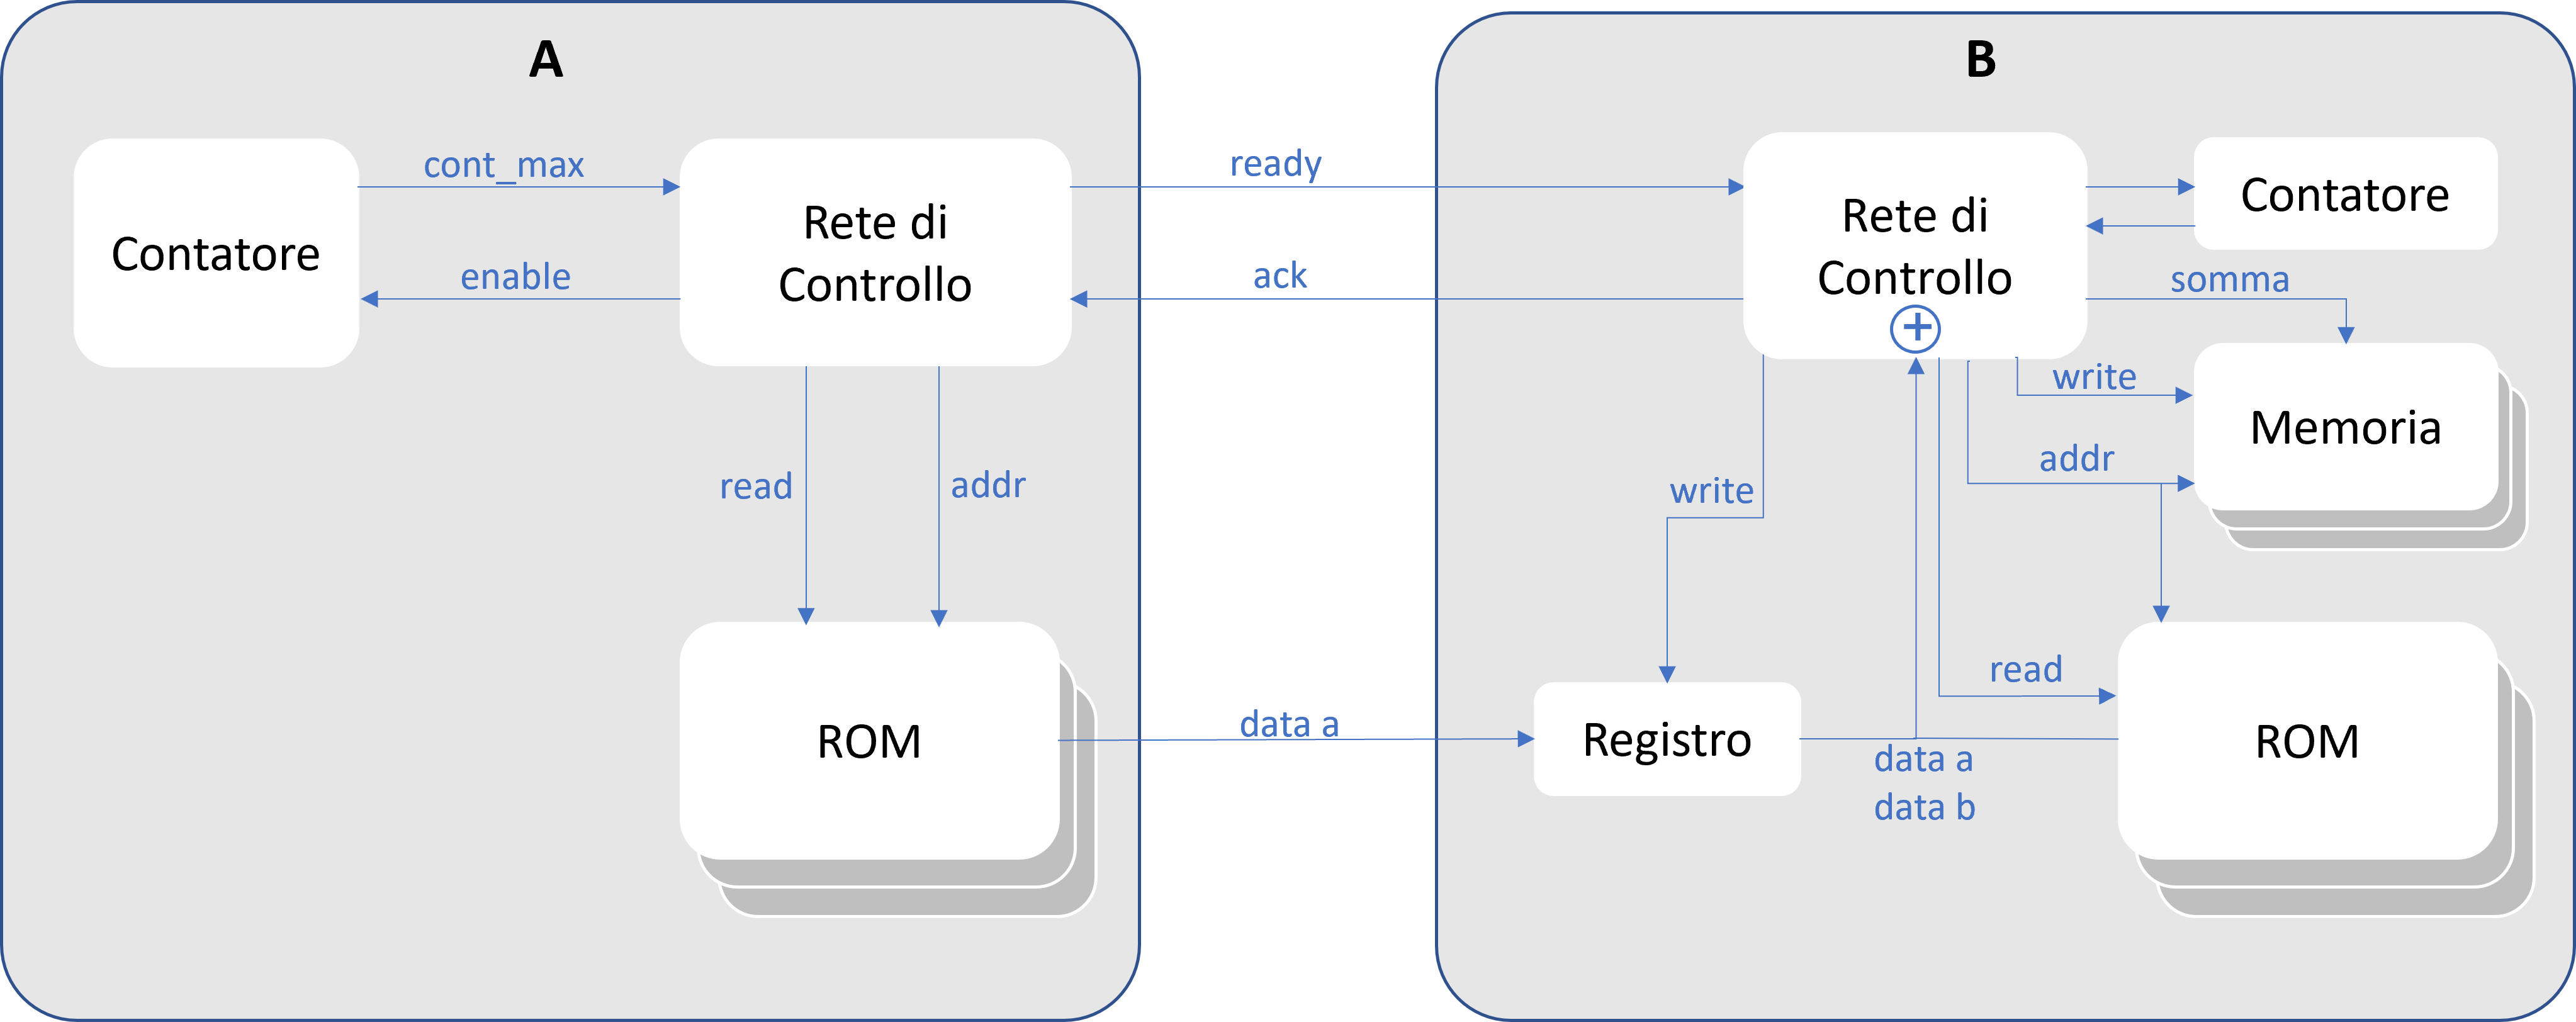
\includegraphics[width=16cm]{immagini/esercizio7/schema_7.1.png}
    \caption{Schema Handshaking}
    \label{fig:my_label}
\end{figure}

Di seguito è possibile osservare la stesura degli automi dei singoli sistemi: 
\begin{figure}[H]
    \centering
    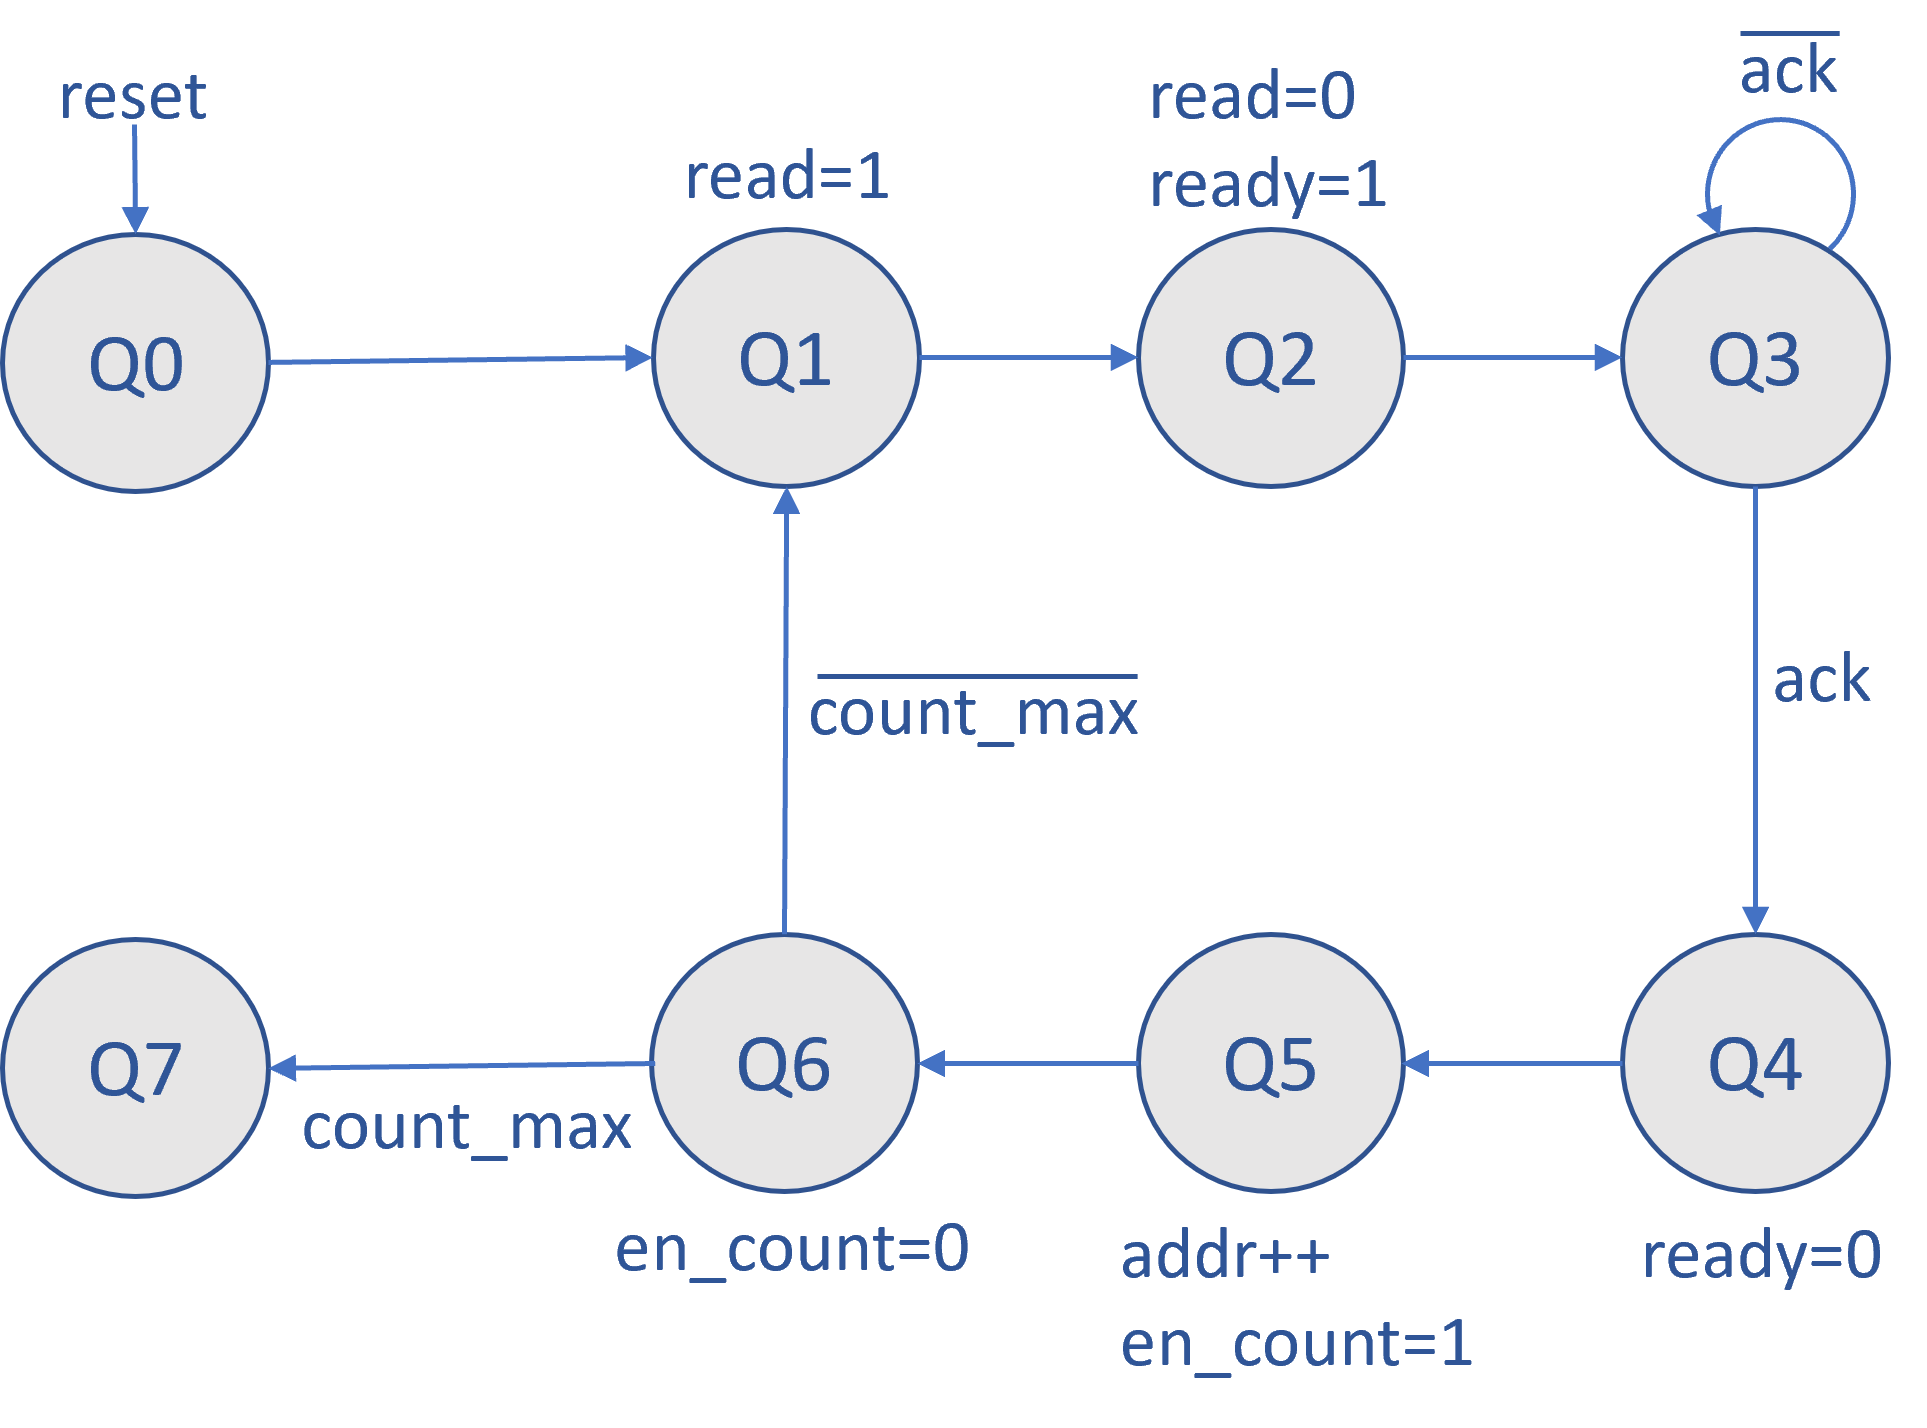
\includegraphics[width=12cm]{immagini/esercizio7/automa_a.png}
    \caption{Automa A}
    \label{fig:7_automa_a}
\end{figure}

\begin{figure}[H]
    \centering
    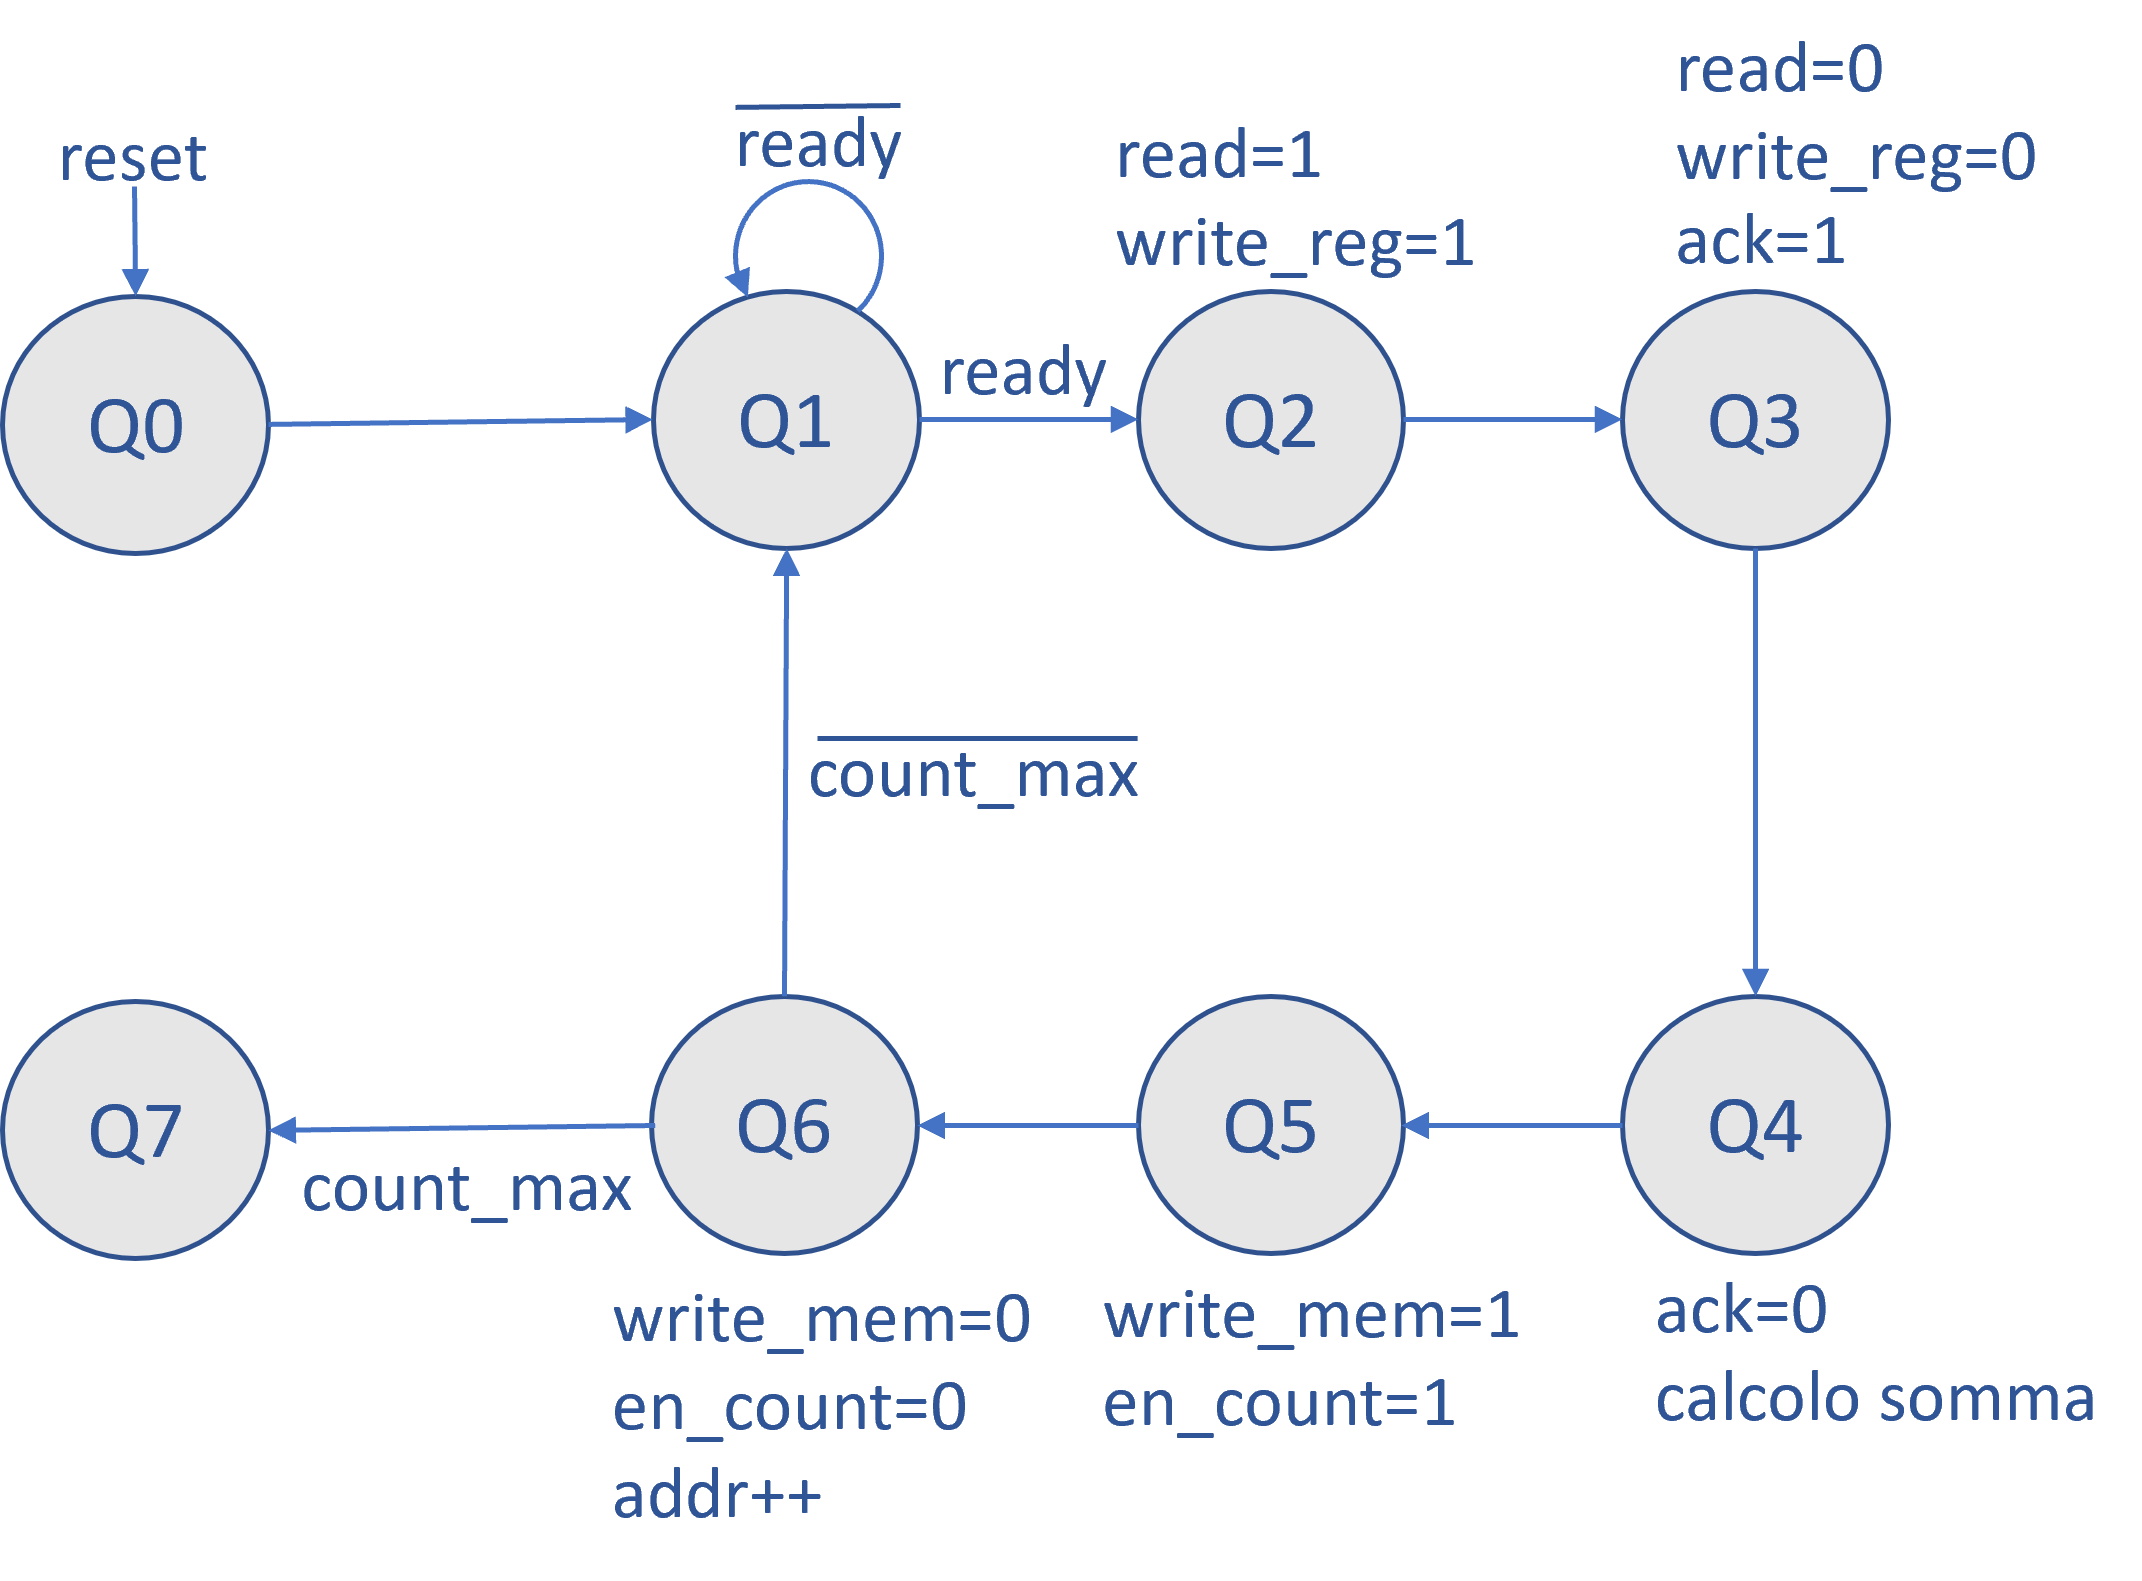
\includegraphics[width=12cm]{immagini/esercizio7/automa_b.png}
    \caption{Automa B}
    \label{fig:7_automa_b}
\end{figure}
Gli stati di particolare interesse sono Q3 per A e Q1 per B. In questi stati infatti si aspetta il segnale generato dall'altro interlocutore, in modo da sincronizzare la comunicazione. Q1 aspetta che il segnale ready sia alzato da A, che indica la possibile trasmissione del dato, Q3 aspetta l'ack che viene alzato da B , che indica l'avvenuta ricezione e scrittura in memoria del dato. I dati vengono memorizzati in un registro temporaneo prima di essere inviati alla rete di controllo per la somma, in modo da poter controllare il momento in cui vengono acquisiti e garantire che non cambino nel tempo.  
Il contatore tiene traccia di quante trasmissioni sono avvenute, e arrivato al massimo invia un segnale \textit{count\_max} che porterà gli automi negli stati Q7, ovvero in idle. 

Sarà necessario un reset per poter ricominciare la trasmissione da capo. 
Un altro aspetto importante riguarda la tempistica con cui si incrementa l'indirizzo addr, necessario a leggere e scrivere nelle memorie dei componenti. Bisogna assicurarsi di completare la scrittura prima dell'incremento, o si rischia di saltare la prima cella di memoria. 
La somma viene effettuata direttamente all'interno del processo della rete di controllo  di B. Tutti gli altri componenti sono stati realizzati a partire da quelli esaminati nei capitoli precedenti, dove è possibile trovarne una descrizione dettagliata.

Di seguito è mostrato il codice dei componenti di A:
\begin{lstlisting} [language=VHDL, caption= Contatore A]
library IEEE;
use IEEE.STD_LOGIC_1164.ALL;
use IEEE.NUMERIC_STD.ALL;

entity contatore is
    Port ( clock : in  STD_LOGIC;
         reset : in  STD_LOGIC;
         enable : in STD_LOGIC;
         counter : out  STD_LOGIC_VECTOR (1 downto 0);
         tc: out std_logic
        );
end contatore;

architecture Behavioral of contatore is

    signal c : std_logic_vector (1 downto 0) := (others => '0');

begin
    counter <= c;
    counter_process: process(clock)
    begin
        if (clock'event AND clock = '1') then
            if (reset = '1') then
                c <= (others => '0');
            else
                if (c="11") then
                    tc<='1';
                elsif (enable='1') then
                    tc<='0';
                    c <= std_logic_vector(unsigned(c) + 1);
                end if;
            end if;
        end if;
    end process;
end Behavioral;


\end{lstlisting}

\begin{lstlisting} [language=VHDL, caption=Rom A]
library ieee;
use ieee.std_logic_1164.all;
use ieee.std_logic_unsigned.all;

entity rom_a is
port(
    clk, read : in std_logic; 
    addr : in std_logic_vector(1 downto 0);
    data : out std_logic_vector(3 downto 0)
    );
end rom_a;

architecture behavioral of rom_a is 
type rom_type is array (0 to 3) of std_logic_vector(3 downto 0);
signal ROM : rom_type := (
    "0010", 
    "0110", 
    "1001", 
    "1111"
);

begin
process(clk)
  begin
    if rising_edge(clk) then
        if read = '1' then
            data <= ROM(conv_integer(addr));
        end if;
    end if;
end process;
end behavioral;
\end{lstlisting}

\begin{lstlisting} [language=VHDL, caption=Rete di controllo A]
library IEEE;
use IEEE.STD_LOGIC_1164.ALL;
use ieee.numeric_std.all;

entity rc_a is
    Port(
        clk,reset,ack: in std_logic;
        count_max :in std_logic;
        en_count,read,ready: out std_logic;
        addr: out std_logic_vector(1 downto 0)
    );
end rc_a;

architecture behavioral of rc_a is

    type stato is (Q0, Q1, Q2, Q3, Q4, Q5, Q6, Q7);
    signal stato_corrente : stato:= Q0;
    signal stato_prossimo : stato;
    signal s_addr: std_logic_vector(1 downto 0) :=(others => '0');

begin
    comb: process(stato_corrente, ack)
       
    begin
        case stato_corrente is
            
            when Q0=>
                stato_prossimo<=Q1;
                s_addr <= "00";
                read<='0';
                ready<='0';
                en_count<='0';

            when Q1=>
                read<='1';
                stato_prossimo<=Q2;

            when Q2=>
                read<='0';
                ready<='1';
                stato_prossimo<=Q3;

            when Q3=>
                if(ack='1') then
                    stato_prossimo<=Q4;
                else
                    stato_prossimo<=Q3;
                end if;

            when Q4=>
                ready<='0';
                stato_prossimo <=Q5;

            when Q5=>
                s_addr <= std_logic_vector( unsigned(s_addr) + 1);
                en_count <='1';
                stato_prossimo <=Q6;

            when Q6=>
                en_count <='0';
                if (count_max ='1') then
                    stato_prossimo <=Q7;
                else
                    stato_prossimo <=Q1;
                end if;

            when Q7=>
                stato_prossimo <=Q7;

            when others => stato_prossimo<= Q0;
        end case;
    end process comb;
 addr <= s_addr;

    seq: process(clk)
    begin
        if rising_edge(clk) then
            if(reset='1')then
                stato_corrente<=Q0;
            else
                stato_corrente<=stato_prossimo;
            end if;
        end if;
    end process seq;
end behavioral;
\end{lstlisting}

Il sistema A, di tipo "Structural", è stato implementato nel seguente modo:
\begin{lstlisting} [language=VHDL, caption= A]
library IEEE;
use IEEE.STD_LOGIC_1164.ALL;

entity A is
    Port (
        clock, ack, reset: in std_logic ;
        ready: out std_logic;
        data: out std_logic_vector (3 downto 0)
    );
end A;

architecture Structural of A is
    component  contatore is
        Port (
            clock : in  STD_LOGIC;
            reset : in  STD_LOGIC;
            enable : in STD_LOGIC;
            counter : out  STD_LOGIC_VECTOR (1 downto 0);
            tc: out std_logic
        );
    end component contatore;

    component rc_a is
        port(
            clk,reset,ack: in std_logic;
            count_max :in std_logic;
            en_count,read,ready: out std_logic;
            addr: out std_logic_vector(1 downto 0)
        );
    end component  rc_a;

    component rom_a is
        port(
            clk, read : in std_logic;
            addr : in std_logic_vector(1 downto 0);
            data : out std_logic_vector(3 downto 0)
        );
    end component  rom_a;

    signal s_count_max:std_logic_vector(1 downto 0):="11";
    signal s_addr:std_logic_vector(1 downto 0):="00";
    signal s_tc, s_en_count, s_read:std_logic :='0';

begin

    CONT : contatore
        port map(
            clock=>clock,
            reset=>reset,
            enable=>s_en_count ,
            tc=>s_tc
        );

    RC : rc_a
        port map(
            clk=>clock,
            reset=>reset,
            ack=>ack,
            en_count=>s_en_count ,
            read=>s_read,
            ready=>ready,
            addr=>s_addr,
            count_max=>s_tc
        );

    ROM : rom_a
        port map(
            clk=>clock,
            read=>s_read,
            addr=>s_addr,
            data=>data
        );
end Structural;
\end{lstlisting}

I componenti del sistema B sono stati implementati tramite un'architettura "Behavioral", di seguito il codice di ognuno di essi:

N.B.: per semplicità è stato omesso il codice del contatore, poiché uguale a quello di A.

\begin{lstlisting} [language=VHDL, caption=Rom B]
library ieee;
use ieee.std_logic_1164.all;
use ieee.std_logic_unsigned.all;

entity rom_b is
Port(
    clk, read : in std_logic; 
    addr : in std_logic_vector(1 downto 0);
    data : out std_logic_vector(3 downto 0)
    );
end rom_b;

architecture behavioral of rom_b is 
type rom_type is array (0 to 3) of std_logic_vector(3 downto 0);
signal ROM : rom_type := (
    "0011", 
    "0111", 
    "0001", 
    "1001"
);

begin
process(clk)
  begin
    if rising_edge(clk) then
        if read = '1' then
            data <= ROM(conv_integer(addr));
        end if;
    end if;
end process;
end behavioral;
\end{lstlisting}

\begin{lstlisting} [language=VHDL, caption=Memoria B]
library ieee;
use ieee.std_logic_1164.all;
use ieee.std_logic_unsigned.all;

entity memoria is
    port(
        clk, write, reset : in std_logic;
        addr : in std_logic_vector(1 downto 0);
        input : in std_logic_vector(4 downto 0);
        output : out std_logic_vector(4 downto 0)
    );
end memoria;

architecture behavioral of memoria is
    type memoria_type is array (0 to 3) of std_logic_vector(4 downto 0);
    signal MEM : memoria_type := (
        "00000",
        "00000",
        "00000",
        "00000"
    );
begin
    process(clk)
    begin
        if rising_edge(clk) then
            if reset = '1' then
                for i in 0 to 3 loop
                    MEM(i) <= "00000";
                end loop;
            elsif write = '1' then
                MEM(conv_integer(addr)) <= input;
            end if;
        end if;
        output<=MEM(conv_integer(addr));
    end process;
end behavioral;
\end{lstlisting}

\begin{lstlisting} [language=VHDL, caption=Registro B]
library IEEE;
use IEEE.STD_LOGIC_1164.ALL;
entity ff is
    port (
        d: in std_logic_vector (3 downto 0);
        clk, reset: in std_logic ;
        write: in std_logic ;
        q:out std_logic_vector (3 downto 0));
end ff;

architecture Behavioral of ff is

begin
    process (clk)
    begin
        if rising_edge (clk) then
            if (reset='1') then
                q<="0000";
            elsif(write='1') then
                q<=d;
            end if;
        end if;
    end process;
end Behavioral;
\end{lstlisting}

\begin{lstlisting} [language=VHDL, caption=Rete di controllo B]
library IEEE;
use IEEE.STD_LOGIC_1164.ALL;
use IEEE.numeric_std.all;

entity rc_b is
    Port (
        clk,reset,ready: in std_logic;
        count_max :in std_logic;
        data_a: in std_logic_vector (4 downto 0);
        data_b: in std_logic_vector (4 downto 0);
        en_count,read,ack,write_mem, write_reg: out std_logic;
        somma: out std_logic_vector(4 downto 0);
        addr: out std_logic_vector(1 downto 0)
    );
end rc_b;

architecture Behavioral of rc_b is

    type stato is (Q0, Q1, Q2, Q3, Q4, Q5, Q6, Q7);
    signal stato_corrente : stato:= Q0;
    signal stato_prossimo : stato;
    signal s_addr: std_logic_vector(1 downto 0) :=(others => '0');
 
begin

    comb: process(stato_corrente, ready)
        variable sum: unsigned(4 downto 0) := (others => '0');
    begin
        case stato_corrente is
        
            when Q0=>
                stato_prossimo<=Q1;
                s_addr <= "00";
                read<='0';
                ack<='0';
                en_count<='0';
                write_mem<='0';
                write_reg<='0';

            when Q1=>
                if(ready='1') then
                    stato_prossimo<=Q2;
                else
                    stato_prossimo<=Q1;
                end if;

            when Q2=>
                read<='1';
                write_reg<='1';
                stato_prossimo<=Q3;

            when Q3=>
                ack<='1';
                read<='0';
                write_reg<='0';
                stato_prossimo<=Q4;

            when Q4=>
                sum:= (unsigned(data_a)+unsigned(data_b));               
                somma<=std_logic_vector(sum);
                ack<='0';
                stato_prossimo <=Q5;

            when Q5=>
                write_mem <='1';
                en_count <='1';
                stato_prossimo <=Q6;      

            when Q6=> 
                write_mem <='0';
                en_count <='0';
                s_addr <= std_logic_vector( unsigned(s_addr) + 1);
                if (count_max ='1') then
                    stato_prossimo <=Q7;
                else
                    stato_prossimo <=Q1;
                end if;

            when Q7=>
                stato_prossimo <=Q7;

            when others => stato_prossimo<= Q0;
        end case;
    end process comb;

    addr <= s_addr;

    seq: process(clk)
    begin
        if rising_edge(clk) then
            if(reset='1')then
                stato_corrente<=Q0;
            else
                stato_corrente<=stato_prossimo;
            end if;
        end if;
    end process seq;

end Behavioral;

\end{lstlisting}

Il sistema B, è stato implementato con il seguente codice:
\begin{lstlisting} [language=VHDL, caption= B]
library IEEE;
use IEEE.STD_LOGIC_1164.ALL;

entity B is
    Port (
        clock, reset , ready: in std_logic ;
        ack: out std_logic ;
        data: in std_logic_vector (3 downto 0)
    );
end B;

architecture Structural of B is
    component  contatore is
        Port (
            clock : in  STD_LOGIC;
            reset : in  STD_LOGIC;
            enable : in STD_LOGIC;
            counter : out  STD_LOGIC_VECTOR (1 downto 0);
            tc: out std_logic
        );
    end component contatore;

    component rom_b is
        port(
            clk, read : in std_logic;
            addr : in std_logic_vector(1 downto 0);
            data : out std_logic_vector(3 downto 0)
        );
    end component  rom_b;

    component ff is
        port (
            d: in std_logic_vector (3 downto 0);
            clk, reset: in std_logic ;
            write: in std_logic ;
            q:out std_logic_vector (3 downto 0));
    end component ff;

    component rc_b is
        Port (
            clk,reset,ready: in std_logic;
            count_max :in std_logic;
            data_a: in std_logic_vector (4 downto 0);
            data_b: in std_logic_vector (4 downto 0);
            en_count,read,ack,write_mem, write_reg: out std_logic;
            somma: out std_logic_vector(4 downto 0);
            addr: out std_logic_vector(1 downto 0)
        );
    end component rc_b;

    component memoria is
        port(
            clk, write, reset : in std_logic;
            addr : in std_logic_vector(1 downto 0);
            input : in std_logic_vector(4 downto 0);
            output : out std_logic_vector(4 downto 0)
        );
    end component memoria;

    signal s_addr:std_logic_vector(1 downto 0):="00";
    signal s_tc, s_en_count, s_read, s_write_mem, s_write_reg:std_logic :='0';
    signal s_data_a, s_data_b: std_logic_vector(3 downto 0):="0000";
    signal s_somma : std_logic_vector(4 downto 0):="00000";
    
begin
    CONT : contatore
        port map(
            clock=>clock,
            reset=>reset,
            enable=>s_en_count ,
            tc=>s_tc
        );

    RC : rc_b
        port map(
            clk=>clock,
            reset=> reset,
            ready=>ready,
            count_max=>s_tc,
            data_a=>'0'&s_data_a,
            data_b=> '0'&s_data_b,
            en_count=>s_en_count,
            read=> s_read ,
            ack=>ack,
            write_mem=> s_write_mem ,
            write_reg=> s_write_reg,
            somma=> s_somma ,
            addr=> s_addr
        );

    ROM : rom_b
        port map(
            clk=>clock,
            read=>s_read,
            addr=>s_addr,
            data=>s_data_b
        );

    MEM: memoria 
        port map(
            clk=> clock ,
            write=> s_write_mem ,
            reset => reset ,
            addr=> s_addr ,
            input=> s_somma 
        );

    REG: ff
        port map(
            d=>data,
            write=>s_write_reg ,
            clk=> clock ,
            reset=> reset,
            q => s_data_a 
        );
end Structural;
\end{lstlisting}

Infine, l'intero sistema di interconnessione AB, di tipo "Structural", è stato implementato nel seguente modo:
\begin{lstlisting} [language=VHDL, caption= AB]
library IEEE;
use IEEE.STD_LOGIC_1164.ALL;
entity AB is
  Port (         
        clock,reset: in std_logic        
  );
end AB;

architecture Structural of AB is

component A is
    Port (
        clock, ack, reset: in std_logic ;
        ready: out std_logic;
        data: out std_logic_vector (3 downto 0)
    );
end component  A;

component B is
    Port (
        clock, reset , ready: in std_logic ;
        ack: out std_logic ;
        data: in std_logic_vector (3 downto 0)
    );
end component B;

signal s_ack, s_ready: std_logic :='0';
signal s_data: std_logic_vector (3 downto 0):="0000";

begin
 sus_A : A
        port map(
            clock=>clock,
            reset=>reset,
            ack=> s_ack  ,
            ready=> s_ready,
            data=>s_data
        );
 sus_B : B
       port map(
            clock=>clock,
            reset=>reset,
            ack=> s_ack  ,
            ready=> s_ready,
            data=>s_data
        );     
end Structural;
\end{lstlisting}

\subsection{Simulazione}
Per una maggiore sicurezza si è scelto di testare prima i sistemi singolarmente e poi di effettuare la simulazione dell'intero sistema di \textit{Handshaking}.

\paragraph{Testbench A}
Per testare il sistema A è stato necessario verificare che l'invio dei dati avvenisse correttamente, ovvero solo dopo aver ricevuto il segnale di ack (simulato). 
\begin{lstlisting} [language=VHDL, caption= Testbench example A]
library IEEE;
use IEEE.STD_LOGIC_1164.ALL;

entity a_tb is
end a_tb;

architecture Behavioral of a_tb is

    component A is
        Port (
            clock, ack, reset: in std_logic ;
            ready: out std_logic;
            data: out std_logic_vector (3 downto 0)
        );
    end component A;

    signal s_clk, s_ack, s_reset, s_ready: std_logic := '0';
    signal s_data: std_logic_vector (3 downto 0);
    constant clk_period: time := 10ns;

begin
    uut: A port map(
            clock=>s_clk,
            ack=>s_ack,
            reset=>s_reset,
            ready=>s_ready,
            data=>s_data
        );

    tb: process
    begin
        wait for 100ns;
        s_reset <='1';
        wait for clk_period;
        s_reset <='0';
             for i in 0 to 3 loop

        wait for 10*clk_period;
        
         s_ack <= '1';
         wait for clk_period;
         s_ack <= '0';

                end loop;
        wait;
    end process tb;

    clock: process
    begin
        loop
            s_clk <= '1';
            wait for clk_period/2;
            s_clk <= '0';
            wait for clk_period/2;
        end loop;
    end process clock;
    
end Behavioral;

\end{lstlisting}

\paragraph{Testbench B}
Per testare il sistema B è stato necessario verificare che la ricezione/memorizzazione dei dati avvenisse correttamente, ovvero solo dopo aver ricevuto il segnale di ready (simulato) e che la rete di controllo prelevasse, sommasse e memorizzasse correttamente gli addendi.
\begin{lstlisting} [language=VHDL, caption= Testbench example B]
library IEEE;
use IEEE.STD_LOGIC_1164.ALL;

entity b_tb is
end b_tb;

architecture Behavioral of b_tb is

    component B is
        Port (
        clock, reset , ready: in std_logic ;
        ack: out std_logic ;
        data: in std_logic_vector (3 downto 0)
    );
    end component B;

    signal s_clk, s_ack, s_reset, s_ready: std_logic := '0';
    signal s_data: std_logic_vector (3 downto 0);
    constant clk_period: time := 10ns;

begin
    uut: B port map(
            clock=>s_clk,
            ack=>s_ack,
            reset=>s_reset,
            ready=>s_ready,
            data=>s_data
        );

    tb: process
    begin
        wait for 100ns;
        s_reset <='1';
        wait for clk_period;
        s_reset <='0';
        
            for i in 0 to 3 loop
        s_data<="0001";
        wait for 4*clk_period;
        s_ready<= '1';        
        wait for clk_period;
        s_ready<= '0';
        wait for 5*clk_period;
              end loop;
        wait;
    end process tb;

    clock: process
    begin
        loop
            s_clk <= '1';
            wait for clk_period/2;
            s_clk <= '0';
            wait for clk_period/2;
        end loop;
    end process clock;
    
end Behavioral;

\end{lstlisting}

\paragraph{Testbench AB}
Infine è stato effettuato il testbench dell'intero sistema di Handshaking. 
\begin{lstlisting} [language=VHDL, caption= Testbench example AB]
library IEEE;
use IEEE.STD_LOGIC_1164.ALL;

entity ab_tb is
end ab_tb;

architecture Behavioral of ab_tb is

   component AB is port (         
        clock,reset: in std_logic        
   );
    end component AB;

    signal s_clk, s_reset: std_logic := '0';
    constant clk_period: time := 10ns;

begin
    uut: AB port map(
            clock=>s_clk,         
            reset=>s_reset
        );

    tb: process
    begin
        wait for 100ns;
        s_reset <='1';
        wait for clk_period;
        s_reset <='0';
        wait for 50*clk_period;
        wait;
    end process tb;

    clock: process
    begin
        loop
            s_clk <= '1';
            wait for clk_period/2;
            s_clk <= '0';
            wait for clk_period/2;
        end loop;
    end process clock;
    
end Behavioral;

\end{lstlisting}

L'output che deriva dal testbench è il seguente:
\begin{figure}[H]
    \centering
    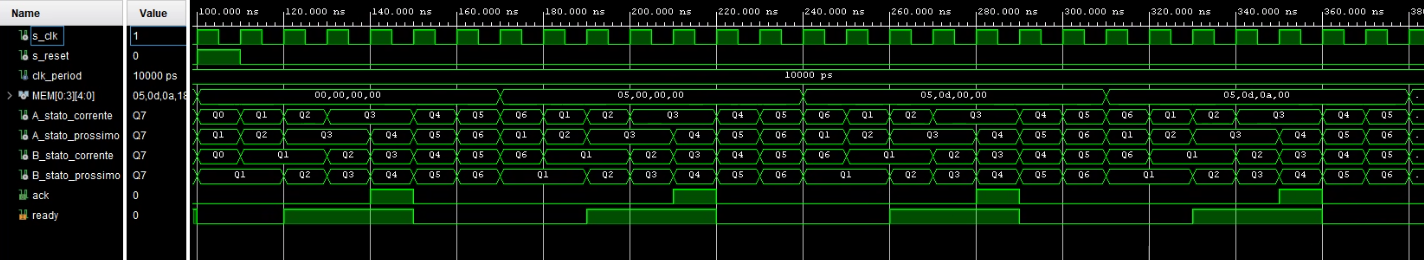
\includegraphics[width=16cm]{immagini/esercizio7/output_simulazione_7.1.png}
    \caption{Output della simulazione}
    \label{fig:notebook}
\end{figure}
\chapter{Processore}

\section{Processore}

A partire dall’implementazione fornita di un processore operante secondo il modello IJVM, 
a)	si proceda all’analisi dell’architettura mediante simulazione e si approfondisca lo studio del suo funzionamento per due istruzioni a scelta, 
b)	si modifichi un codice operativo a scelta, documentando tutte le modifiche effettuate,
c)	(opzionale) si descriva il funzionamento del processore in merito alle istruzioni di input/output,
d)	(solo ove possibile) si sintetizzi il processore su FPGA.

\subsection{Architettura MIC-1}
Il processore MIC-1 è caratterizzato da un'architettura a stack, composta da due componenti principali: control unit e datapath.
Lo stack permette di memorizzare i diversi operandi necessari alle varie operazioni e si trova in memoria. Per poterlo utilizzare sono necessari due registri, lo \textit{Stack Pointer(SP)} (che punta sempre all'ultimo elemento inserito nello stack) e il \textit{Top Of Stack (TOS)} (il valore puntato). 

Di seguito viene mostrato uno schema dell'architettura generale.
\begin{figure}[H]
    \centering
    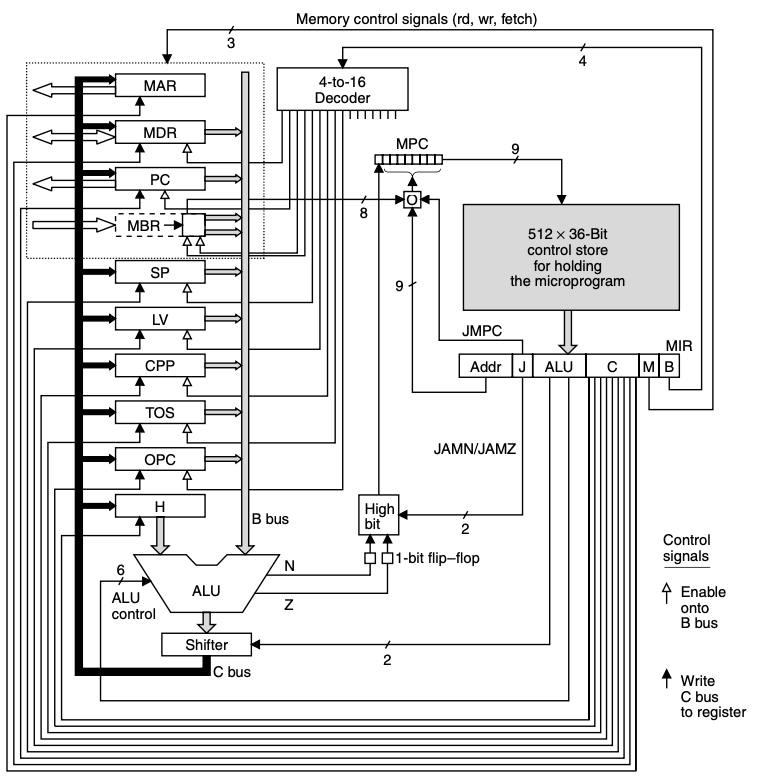
\includegraphics[width=16cm]{immagini/esercizio8/mic1_arch.png}
    \caption{Architettura MIC-1}
    \label{fig:mic1_arch}
\end{figure}

\subsubsection{Control Unit}
La \textit{control unit} stabilisce qual è la prossima microistruzione da prendere dalla ROM e, conoscendo il suo formato, si occupa di abilitare i segnali appropriati del datapath.
In particolare, il microprogramma è memorizzato nella ROM 512x36 chiamata Control Store, e per potervi accedere si utilizza il registro,\textit{ MPC (MicroProgram Counter)}. 
Ciascuna microistruzione (Control Word) è composta da 36 bit ed è strutturata come mostrato in figura:

\begin{figure}[H]
    \centering
    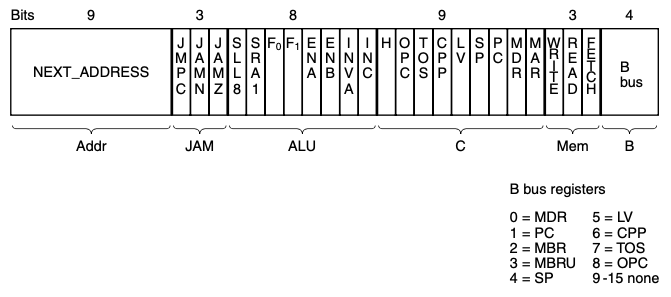
\includegraphics[width=16cm]{immagini/esercizio8/mic1_instr.png}
    \caption{Formato microistruzione del MIC-1}
    \label{fig:mic1_instr}
\end{figure}

Di seguito sono descritti i vari campi della Control Word:
\begin{itemize}
\item Addr: Indirizzo a 9 bit di una potenziale prossima microistruzione da inserire nel MPC. Questo indirizzo viene combinato con i segnali \textit{N} e \textit{Z} (in uscita dall'ALU) e \textit{JAMN}, \textit{JAPZ} e \textit{JMPC} per effettuare eventuali salti. 
\item JAM: I tre bit della sezione JAM specificano eventuali salti  che alterano il flusso lineare dell'indirizzamento in memoria;
\item ALU: Controllo dell'ALU e dello shifter con cui specificare le operazioni da svolgere. In particolare, l'ALU è controllata da 6 bit ed è alimentata dal bus B e dal registro H, mentre lo \textit{shifter} viene controllato da 2 bit.
\item C: Controlla quali registri vengono scritti dal bus C. Il bus C è in lettura e viene controllato esplicitamente da 9 bit. Questa scelta da la possibilità di scrivere i valori in più registri contemporaneamente.
\item Mem: Tre bit per controllare le operazioni di memoria. Pur avendo 2 coppie di registri MAR-MDR (che usano parole da 32 bit) e PC-MBR (che usano parole da 8 bit) sono necessari solo 3 bit poiché l'operazione di scrittura non ha senso per il \textit{Program Counter}.
\item B: Seleziona il registro connesso al bus B. Essendo un bus di scrittura, e quindi accessibile \textbf{solo} in mutua esclusione dai registri del \textit{datapath}, è conveniente effettuare una codifica dei segnali di abilitazione per rendere la memoria più piccola. In particolare, essendo 9 i registri che devono scrivere, è necessaria una codifica su 4 bit. Questa scelta comporta l'introduzione di un \textit{decoder} 4-16 nell'architettura.
\end{itemize}


\subsubsection{Datapath}
Il datapath è costituito da 9 registri, un ALU e uno \textit{shift register} controllati attraverso due bus separati: il bus B, necessario alla scrittura, e il bus C per la lettura.

L'ALU ha i seguenti ingressi:
\begin{itemize}
    \item A: collegato al registro H;
    \item B: collegato al bus B;
    \item Controlli: 6 segnali provenienti dall'unità di controllo;
\end{itemize}

Mentre fornisce le seguenti uscite:
\begin{itemize}
    \item N: bit alto se il risultato è negativo;
    \item Z: bit alto se il risultato è zero;
    \item OUT: risultato delle operazioni che viene messo in ingresso allo \textit{shift register};
\end{itemize}

\subsubsection{Interazione con la memoria}
Ci sono una serie di registri adibiti alla comunicazione con la memoria. Come detto in precedenza, sono controllati dai segnali MEM\_X presenti nelle micro-istruzioni. In particolare, si dividono in due coppie:
\begin{itemize}
    \item MAR-MDR: registri a 32 bit che servono a leggere e scrivere dalla memoria. In particolare, il MAR contiene l'indirizzo con cui avverrà la lettura/scrittura; mentre in MDR sarà presente il dato letto/scritto. Inoltre, la scrittura avviene in un colpo di clock ed è necessario fornire un segnali di abilitazione; invece la lettura avviene in due colpi di clock e non è necessario un'abilitazione;
    \item MBR-PC: registri a 8 bit da cui è possibile solo leggere byte dalla memoria. Per questo motivo, una microistruzione può portare più accessi in memoria;
\end{itemize}
\begin{figure}[H]
    \centering
    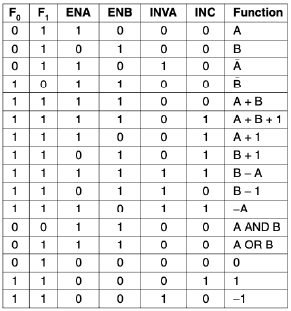
\includegraphics[width=10cm]{immagini/esercizio8/ALU.png}
    \caption{Tabella delle operazioni ALU}
    \label{fig:alu}
\end{figure}


\subsubsection{Analisi BIPUSH}
In questa sezione viene esaminata il codice operativo BIPUSH, analizzando le singole microistruzioni.

BIPUSH = 0x10:
\begin{enumerate}
\item SP = MAR = SP + 1 : in questa microistruzione viene incrementato lo stack pointer e il nuovo indirizzo viene caricato all'interno del MAR, in modo da specificare la locazione di memoria dove inserire il nuovo dato.
\item PC = PC + 1; fetch : questa microistruzione è presente in ogni codice operativo e serve a prepararsi per la prossima operazione.
\item MDR = TOS = MBR; wr; goto main : l'operando memorizzato nell'MBR viene inserito nel TOS che a sua volta viene inserito nel MDR. Successivamente, col segnale wr, viene abilitata la scrittura. 

\end{enumerate}
Ognuna delle microistruzioni viene rappresentata da una stringa di 36 bit, come descritto in precedenza, e nel caso della BIPUSH la prima è composta dai seguenti campi:
\begin{itemize}
    \item  ADDR: 000010001
    \item JAM: 000
    \item Shift Register: 00
    \item ALU: 110101
    \item C: 000001001
    \item Mem: 000
    \item B: 0100
\end{itemize}

In Figura \ref{fig:bipush_sim}, è mostrato il risultato della simulazione quando viene eseguito il seguente programma:

\begin{lstlisting} [language=ant, caption=Programma simulazione BIPUSH]
main
.var
a
.endvar
BIPUSH 0xA
HALT
.endmethod
\end{lstlisting}

\begin{figure}[H]
    \centering
    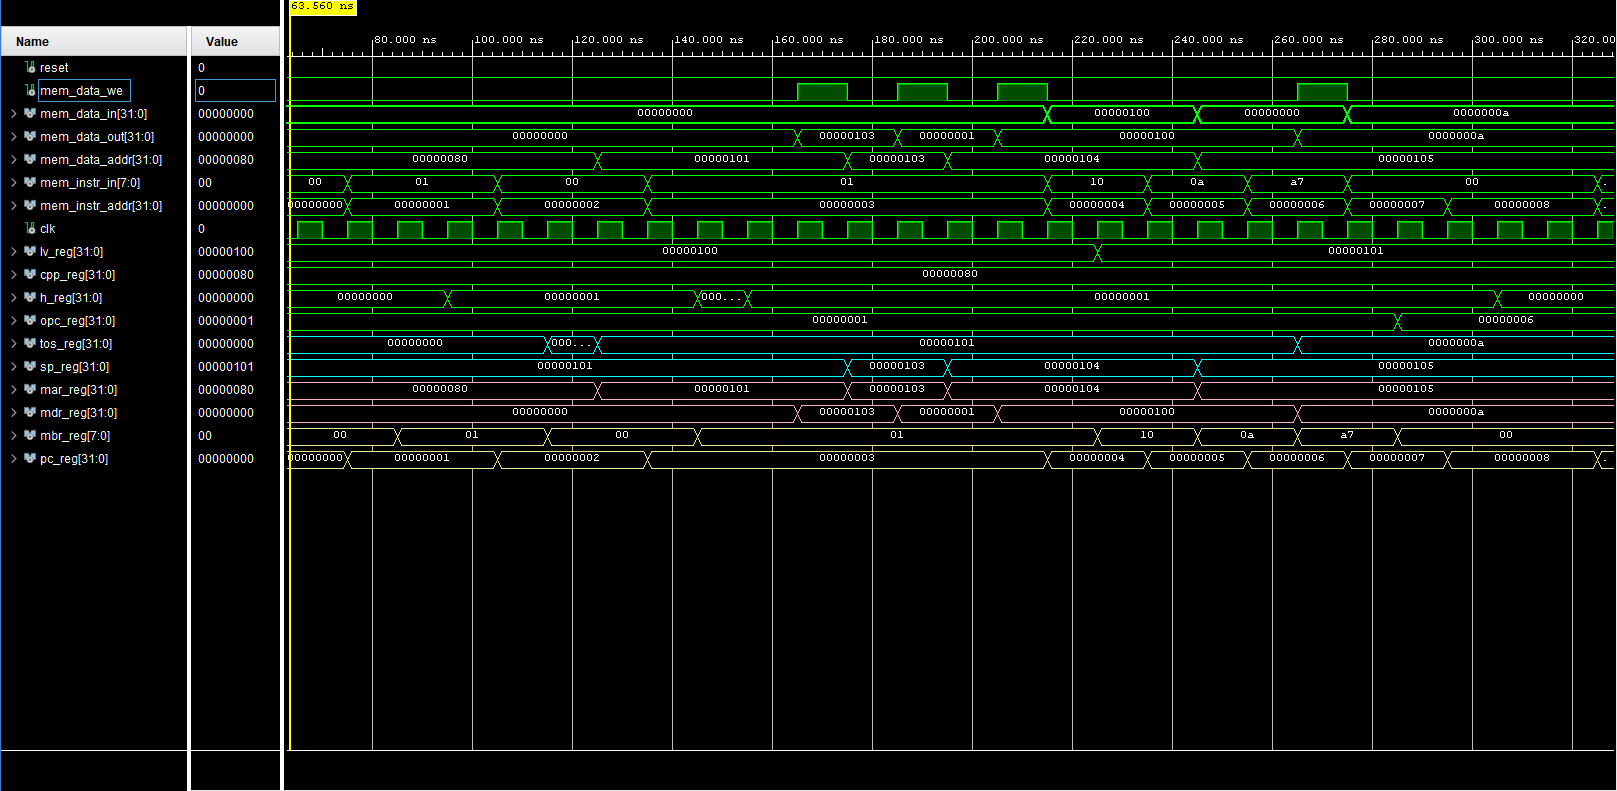
\includegraphics[width=17cm]{immagini/esercizio8/bipush_sim.png}
    \caption{Simulazione BIPUSH}
    \label{fig:bipush_sim}
\end{figure}

\subsubsection{Analisi IADD}
In questa sezione, si è scelto di esaminare il codice operativo IADD.
iadd = 0x65:
\begin{enumerate}
\item MAR = SP = SP - 1; rd: lettura del penultimo elemento dello stack.
\item H = TOS: salvataggio temporaneo di TOS in H
\item MDR = TOS = MDR+H: salvataggio in MDR e TOS della somma.

\end{enumerate}
Anche in questo codice operativo viene mostrato di seguito un esempio di rappresentazione binaria della prima microistruzione:
\begin{itemize}
    \item ADDR: 010011010
    \item JAM: 000
    \item Shift Register: 00
    \item ALU: 110110
    \item C: 000001001
    \item Mem: 010
    \item B: 0100
\end{itemize}

In Figura \ref{fig:bipush_sim}, è mostrato il risultato della simulazione quando viene eseguito il seguente programma:

\begin{lstlisting} [language=ant, caption=Programma simulazione IADD]
.main
.var
a
.endvar
BIPUSH 0xA
BIPUSH 0xE
IADD
ISTORE a
HALT
.endmethod
\end{lstlisting}



\begin{figure}[H]
    \centering
    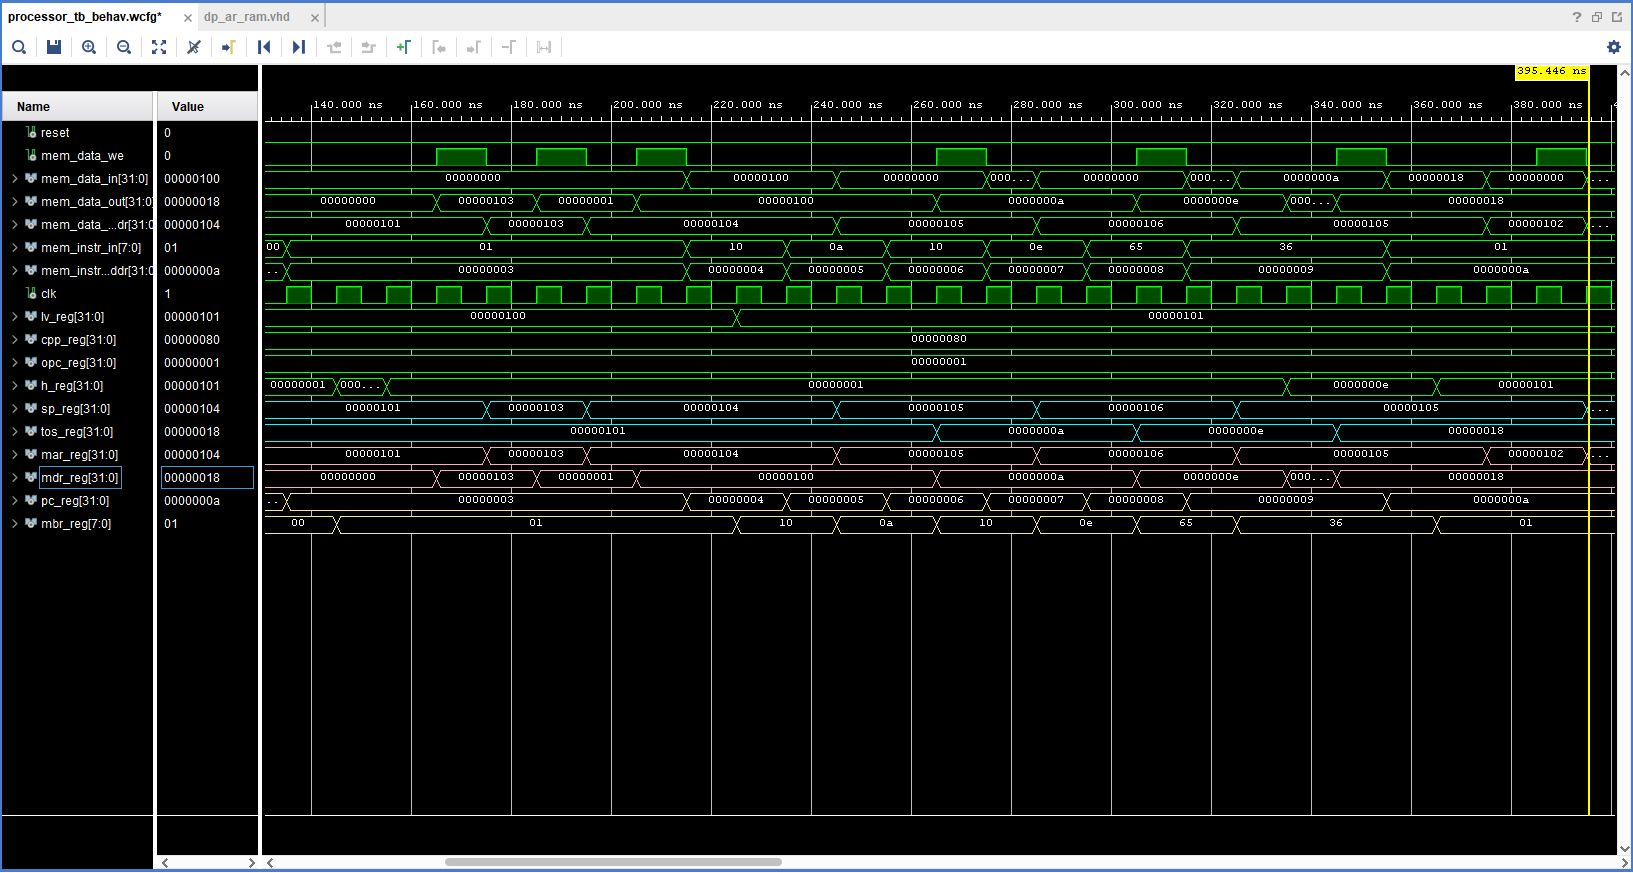
\includegraphics[width=17cm]{immagini/esercizio8/iadd_sim.png}
    \caption{Simulazione IADD}
    \label{fig:iadd_sim}
\end{figure}

\subsection{Modifica codice operativo IADD}
Per modificare il codice operativo sono stati innanzitutto installati i tool necessari a ricompilare le parti cambiate ovvero:\textit{Control Store}e \textit{la Memoria}. In particolare, è stato preso il codice operativo IADD ed è stata modificata la terza microistruzione: 

\begin{lstlisting} [language=ant, caption=Codice operativo IADD modificato in ISUB]
iadd = 0x65:
        MAR = SP = SP - 1; rd
        H = TOS
        MDR = TOS = MDR - H; wr; goto main
\end{lstlisting}

In questo modo invece di sommare \textit{H} a \textit{MDR} viene eseguita una sottrazione, infatti è possibile notare nel testbench qui riportato il nuovo valore del risultato in \textit{mem\_data\_out}:

\begin{figure}[H]
    \centering
    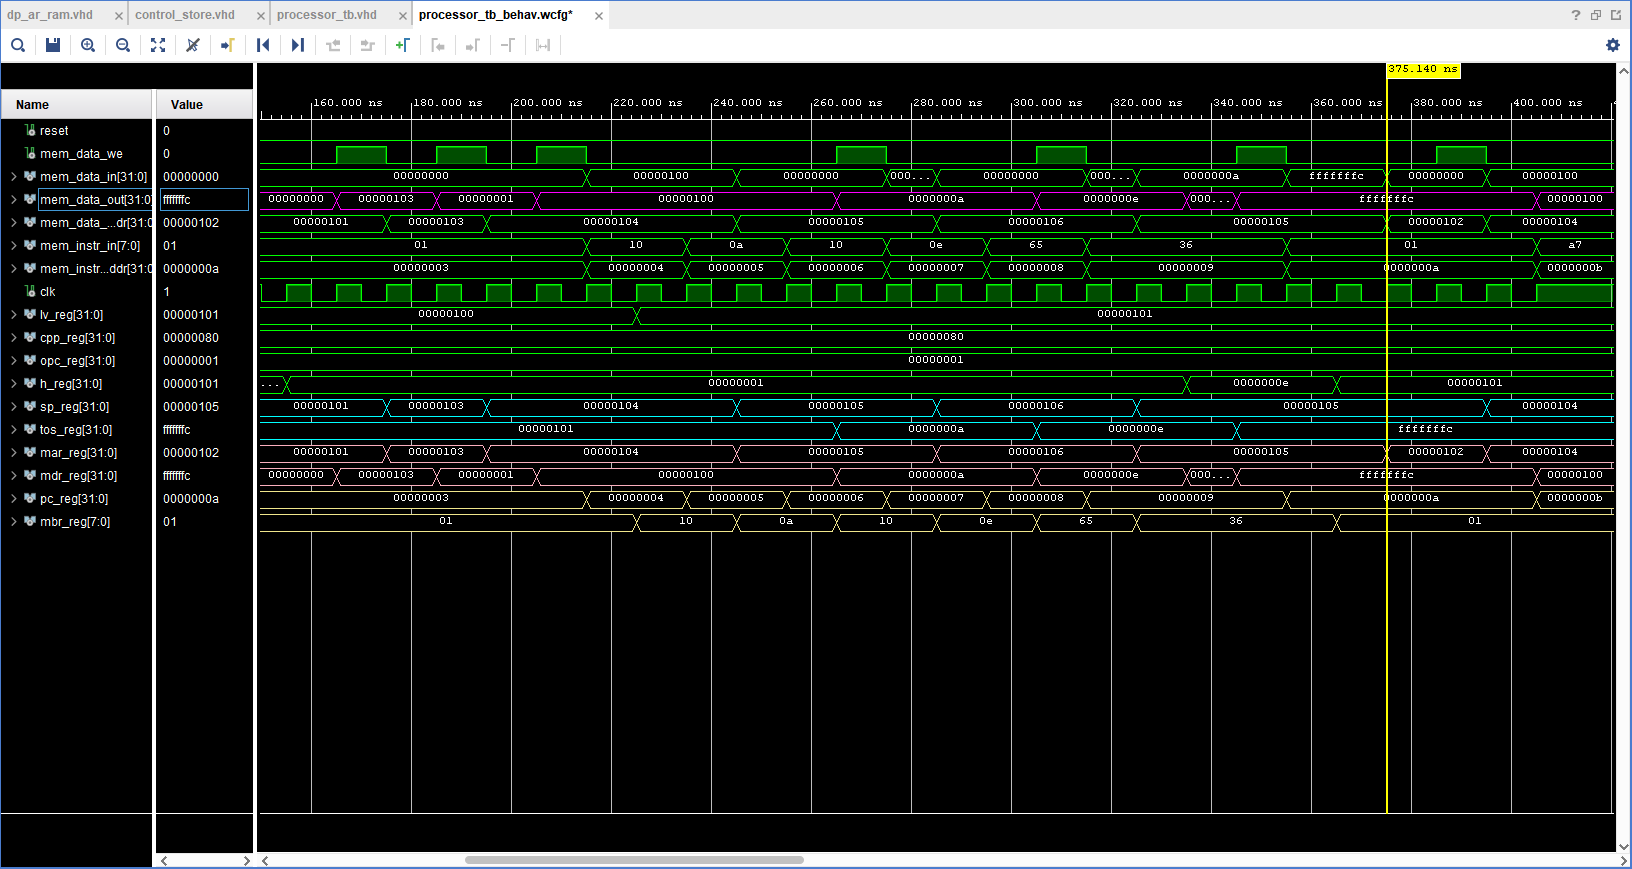
\includegraphics[width=17cm]{immagini/esercizio8/iadd_mod_sim.png}
    \caption{Simulazione IADD modificata in ISUB}
    \label{fig:iadd_imod}
\end{figure}




\chapter{Interfaccia seriale}

\section{UART}

Sfruttando l’implementazione fornita dalla Digilent di un dispositivo UART (componente RS232RefComp.vhd), progettare e implementare in VHDL un sistema costituito da 2 nodi A e B collegati tra loro mediante una interfaccia seriale. Il sistema A acquisisce una stringa di 8 bit dall’utente (mediante gli switch della board di sviluppo) e la invia mediante la seriale al sistema B, che la manda in output sui led della board di sviluppo. 

\subsection{Descrizione UART}
Il dispositivo UART della Digilent è in grado di operare in modalità \textit{full duplex}, ed è formata da due componenti principali: un trasmettitore e un ricevitore.
La frame dei dati utilizzata per la trasmissione prevede due bit per marcare l'inizio e la fine del messaggio, e otto bit per i dati effettivi.


\begin{figure}[H]
    \centering
    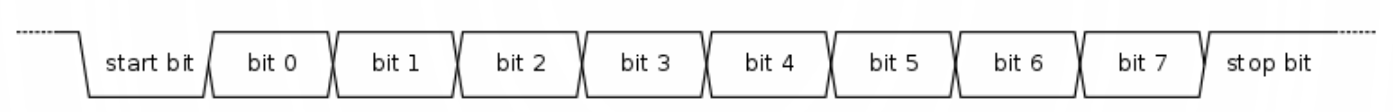
\includegraphics[width=17cm]{immagini/esercizio9/frame.png}
    \caption{Frame UART}
    \label{fig:my_label}
\end{figure}

Lo stato di inattività viene mostrato da un bit alto, in modo da poter constatare in ogni caso il corretto funzionamento del sistema senza creare ambiguità (se fosse basso non sarebbe possibile distinguere il caso di non trasmissione da quello di linea interrotta).

Il ricevitore ha il compito di prendere i dati seriali in ingresso e convertirli in parallelo. Un registro a scorrimento viene utilizzato per memorizzare i dati in ingresso sulla porta \textit{RXD}. Un controller si occupa di gestire i segnali tra i diversi componenti e genera l'uscita \textit{RDA} per notificare la fine della ricezione. Lo schema dell'automa del controller è mostrato nella figura.

\begin{figure}[H]
    \centering
    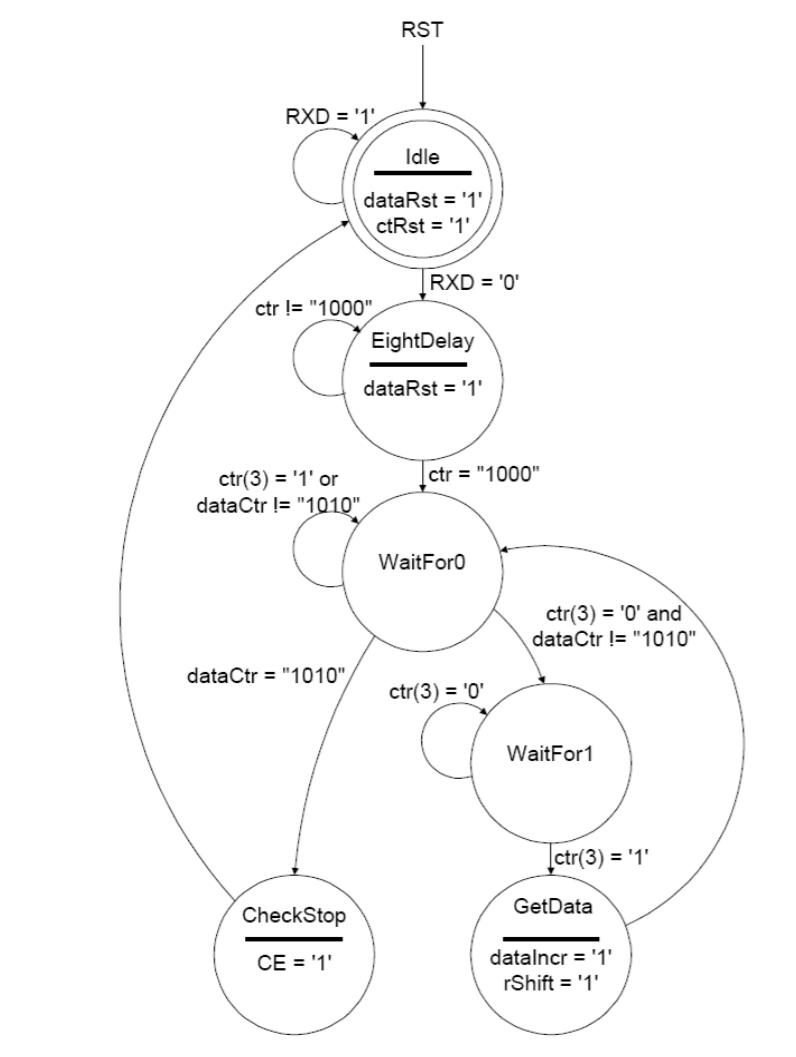
\includegraphics[width=11cm]{immagini/esercizio9/ricevitore_automa.png}
    \caption{Automa Ricevitore}
    \label{fig:my_label}
\end{figure}

Il trasmettitore ha il compito di prendere i dati paralleli in input e inviarli uno alla volta sull'uscita \textit{TXD}. Anche questo componente ha un controller che gestisce la velocità di trasmissione e il numero dei bit inviati. Lo schema dell'automa del controller è mostrato in figura. 

\begin{figure}[H]
    \centering
    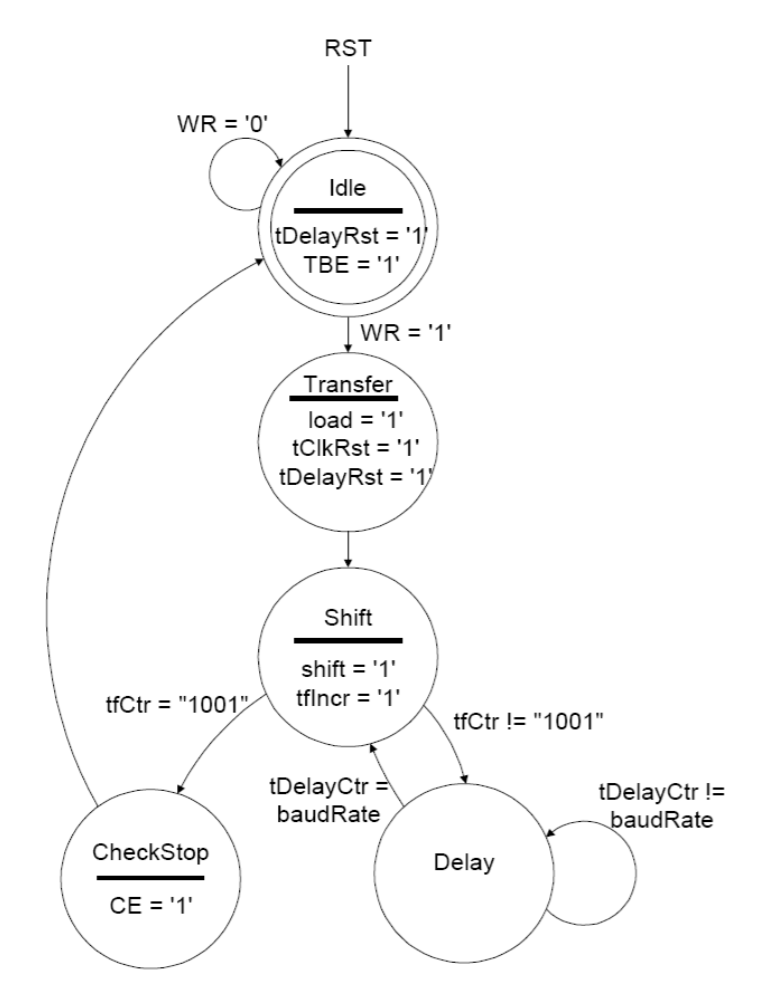
\includegraphics[width=11cm]{immagini/esercizio9/trasmettitore_automa.png}
    \caption{Automa Trasmettitore}
    \label{fig:my_label}
\end{figure}
Il ricevitore e il trasmettitore non condividono normalmente lo stesso clock, per cui viene stabilito il numero di transizioni con il \textit{baud rate}. Questo può essere calcolato come:
\begin{equation*}
    \frac{frequenza\;clock}{baud}
\end{equation*}

dove il baud è uguale a 115200. La frequenza del ricevitore, che deve sovra-campionare la linea in modo da essere 16 volte più veloce del trasmettitore, può essere ottenuta con il \textit{baud divide}, calcolabile come:
\begin{equation*}
    \frac{baud\;rate\;clock}{16}
\end{equation*}

\subsection{Architettura}

La soluzione è stata realizzata seguendo un approccio strutturale, partendo dalla creazione dei due sistemi separati, A e B, e procedendo con l'interconnessione di essi. 

Il sistema A è composto da:
\begin{itemize}
    \item \textit{registro}: un flip flop che memorizza la stringa inserita dall'utente;
    \item \textit{UART}: il componente, fornitoci a priori, costituisce in un'interfaccia per la trasmissione del dato tra i due sistemi;
    \item \textit{rete di controllo}: regola che la trasmissione dei dati avvenga in modo corretto.
\end{itemize}

Il sistema B, invece, è composto da:
\begin{itemize}
    \item \textit{registro}: un flip flop che memorizza la stringa ricevuta dal sistema A, che esce dal ricevitore UART;
    \item \textit{UART}: il componente, fornitoci a priori, costituisce in un'interfaccia per la ricezione della stringa;
    \item \textit{rete di controllo}: regola che la trasmissione e l'output dei dati avvenga in modo corretto.
\end{itemize}

Le interconnessioni tra i due sistemi sono visibili nella seguente architettura: 
\begin{figure}[H]
    \centering
    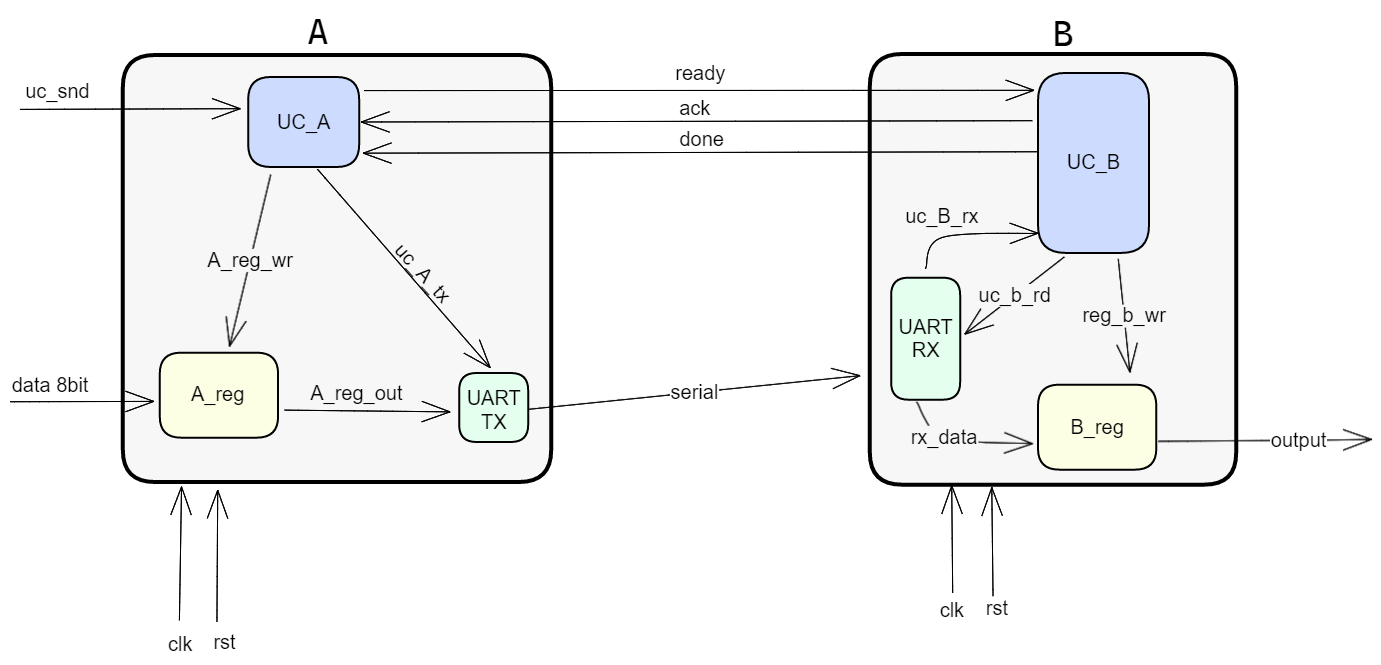
\includegraphics[width=18cm]{immagini/esercizio9/schema_9.1.png}
    \caption{Schema Interfaccia Seriale}
    \label{fig:my_label}
\end{figure}
I componenti registro e UART sono basati su quelli descritti nelle sezioni precedenti.
Le reti di controllo di A e B si occupano di gestire non solo i componenti del proprio sistema, ma comunicano tra loro in modo da sincronizzare l'inizio e la fine della trasmissione.
Anche se non richiesto dalla traccia, è stata inserita una logica di handshaking a 3 passaggi (three way handshaking) in modo da assicurarsi non solo che tutti e due i dispositivi siano pronti alla trasmissione, ma che il dato arrivi a destinazione nella sua interezza. Questo è particolarmente importante dato che il ricevitore deve essere già pronto quando il trasmettitore inizia a inviare. 
Questa aggiunta è stata utile anche per sperimentare metodi di controllo più avanzati della seriale, che sono stati poi utilizzati nell'esercizio a scelta finale, ed è stata fatta in questo esercizio e non nel successivo (9.2) per iniziare a testarlo con un sistema meno complesso.

Nell'automa di A ci sono tre condizioni che bloccano il sistema con un auto-anello: innanzitutto deve arrivare il segnale di \textit{send} dall'esterno, per iniziare il processo di trasmissione, in seguito il sistema alza il segnale \textit{ready} e aspetta l'ack di B. Una volta arrivato l'ack inizia la trasmissione con la UART, alzando il segnale uc\_A\_tx, e si aspetta che B riceva l'intero messaggio e alzi il segnale \textit{done}.


Nell'automa di B ci sono due auto-anelli: il primo aspetta che A alzi il segnale di \textit{ready}, in modo da poter mandare l'\textit{ack} e in seguito si aspetta che la periferica UART alzi il segnale \textit{uc\_B\_rx}, detto anche RDA. Questo segnale indica la fine della ricezione del messaggio, per cui sarà possibile scrivere il risultato nel registro e confermare la fine della trasmissione alzando il \textit{done}.

Di seguito è possibile osservare la stesura degli automi dei singoli sistemi: 

\begin{figure}[H]
    \centering
    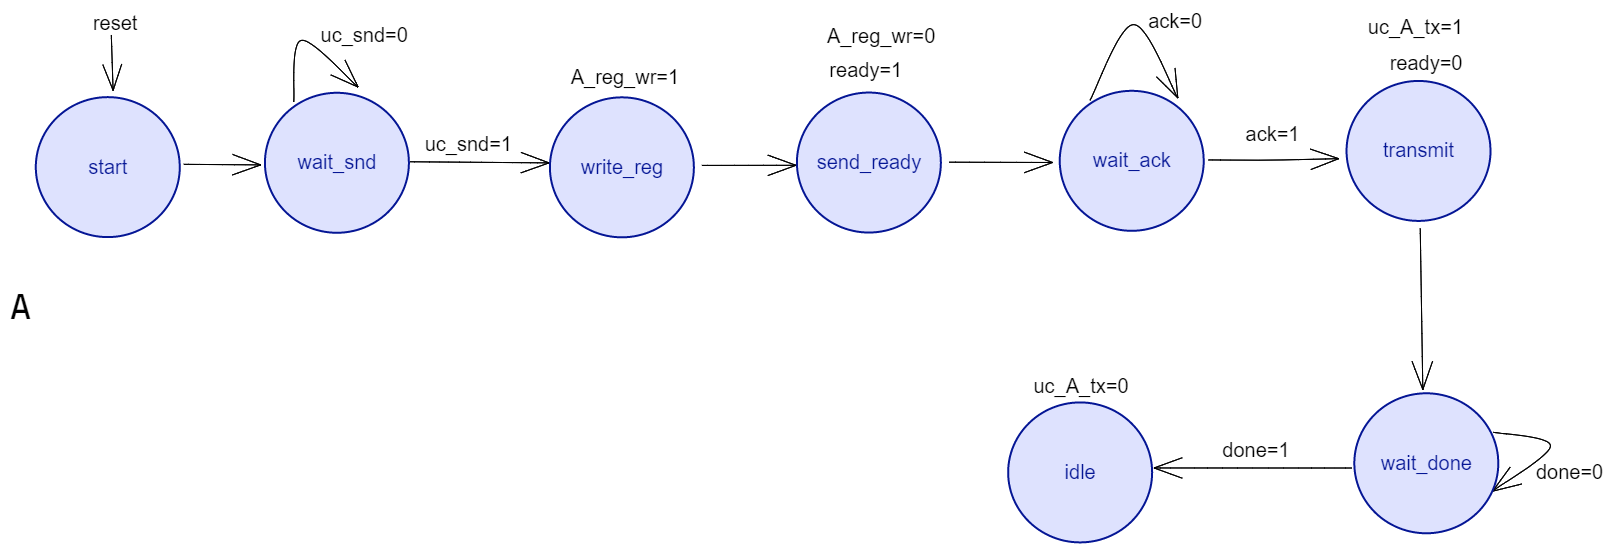
\includegraphics[width=17cm]{immagini/esercizio9/automaA_9.1.png}
    \caption{Automa A}
\end{figure}

\begin{figure}[H]
    \centering
    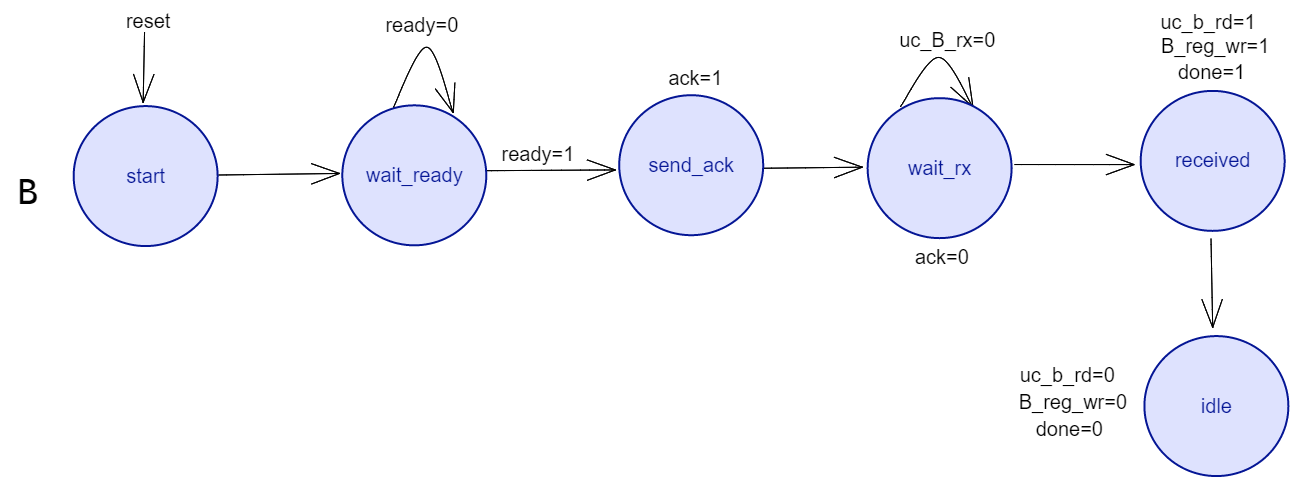
\includegraphics[width=17cm]{immagini/esercizio9/automaB_9.1.png}
    \caption{Automa B}
\end{figure}


Di seguito è mostrato il codice dei sistemi A e B.
N.B.: per semplicità è stato omesso il codice della UART.

\begin{lstlisting} [language=VHDL, caption=Registro]
library IEEE;
use IEEE.STD_LOGIC_1164.ALL;

entity reg is
    Port (
        din: in std_logic_vector(7 downto 0);
        clk, rst, wr: in std_logic;
        dout: out std_logic_vector(7 downto 0)
       );
end reg;

architecture Behavioral of reg is
begin
    ff: process(clk)
        begin
            if rising_edge(clk) then
                if rst = '1' then
                    dout <= (others => '0');
                elsif wr = '1' then
                    dout <= din;
                end if;
            end if;
    end process ff;
end Behavioral;
\end{lstlisting}

\begin{lstlisting} [language=VHDL, caption=Rete di controllo di A]
library IEEE;
use IEEE.STD_LOGIC_1164.ALL;
use IEEE.std_logic_unsigned.all;

entity uc_a is
    port(
        clk, rst, ack, done, uc_snd: in std_logic;
        ready, uc_a_tx, reg_a_wr : out std_logic
    );
end uc_a;

architecture behavioral of uc_a is

    type state is (
        IDLE,
        START,
        WAIT_SND,
        WRITE_REG,
        SND_READY,
        WAIT_ACK,
        TRANSMIT,
        WAIT_DONE
    );
    
    signal current_state : state:= IDLE;
    signal next_state : state;
  
begin
    comb: process(current_state, ack, done, uc_snd)
    begin
        case current_state is
        
            when START =>
                ready <= '0';
                uc_a_tx <= '0';
                reg_a_wr <= '0';
                next_state<= WAIT_SND;
                
            when WAIT_SND=>
                if ( uc_snd = '1' ) then
                    next_state <= WRITE_REG;
                else
                    next_state <= WAIT_SND;
                end if;
                
            when WRITE_REG=>
                reg_a_wr <= '1';
                next_state <= SND_READY;
                
            when SND_READY=>
                reg_a_wr <= '0';
                ready <= '1';
                next_state <= WAIT_ACK;
                
            when WAIT_ACK=>
                if ( ack = '1' ) then
                    next_state <= TRANSMIT;
                else
                    next_state <= WAIT_ACK;
                end if;
                
            when TRANSMIT=>
                uc_a_tx <= '1';
                ready <= '0';
                next_state <= WAIT_DONE;
                
            when WAIT_DONE=>
                if ( done = '1' ) then
                    next_state <= IDLE;
                else
                    next_state <= WAIT_DONE;
                end if;
                
            when IDLE=>
                uc_a_tx <= '0';
                
            when others => next_state<= IDLE;
        end case;
    end process comb;

    seq: process(clk)
    begin
        if rising_edge(clk) then
            if rst='1'  then
                current_state<=START;
            else
                current_state<=next_state;
            end if;
        end if;
    end process seq;
    
end behavioral;
\end{lstlisting}

Di seguito il codice di A:
\begin{lstlisting} [language=VHDL, caption=Sistema A]
library IEEE;
use IEEE.STD_LOGIC_1164.ALL;

entity a is
 Port (
    uc_snd, clk, rst, ack, done: in std_logic;
    data : in std_logic_vector(7 downto 0);
    output, ready: out std_logic
  );
end a;

architecture Structural of a is

component UARTcomponent is
	Generic (
		--@48MHz
--		BAUD_DIVIDE_G : integer := 26; 	--115200 baud
--		BAUD_RATE_G   : integer := 417

		--@26.6MHz
		BAUD_DIVIDE_G : integer := 14; 	--115200 baud
		BAUD_RATE_G   : integer := 231
	);
	Port (	
		TXD 	: out 	std_logic  	:= '1';					-- Transmitted serial data output
		RXD 	: in  	std_logic;							-- Received serial data input
		CLK 	: in  	std_logic;							-- Clock signal
		DBIN 	: in  	std_logic_vector (7 downto 0);		-- Input parallel data to be transmitted
		DBOUT 	: out 	std_logic_vector (7 downto 0);		-- Recevived parallel data output
		RDA		: inout  std_logic;							-- Read Data Available
		TBE		: out 	std_logic 	:= '1';					-- Transfer Buffer Emty
		RD		: in  	std_logic;							-- Read Strobe
		WR		: in  	std_logic;							-- Write Strobe
		PE		: out 	std_logic;							-- Parity error		
		FE		: out 	std_logic;							-- Frame error
		OE		: out 	std_logic;							-- Overwrite error
		RST		: in  	std_logic	:= '0');				-- Reset signal
						
end component  UARTcomponent;

component uc_a is
    port(
        clk, rst, ack, done, uc_snd: in std_logic;
        ready, uc_a_tx, reg_a_wr : out std_logic
    );
end component uc_a;

component reg is
    Port (
        din: in std_logic_vector(7 downto 0);
        clk, rst, wr: in std_logic;
        dout: out std_logic_vector(7 downto 0)
       );
end component reg;

signal reg_a_wr, uc_a_tx: std_logic;
signal reg_a_out: std_logic_vector(7 downto 0);

begin

a_reg: reg port map(
    din=>data,
    clk=>clk,
    rst=>rst,
    wr=>reg_a_wr,
    dout => reg_a_out
);

cu: uc_a port map(
    clk=>clk,
    rst=>rst,
    done=>done,
    ack=>ack,
    ready=>ready,
    uc_a_tx=> uc_a_tx,
    uc_snd=> uc_snd,
    reg_a_wr=>reg_a_wr
);

uart:  UARTcomponent generic map(
    BAUD_DIVIDE_G=>26,
    BAUD_RATE_G=>417
)
port map (
    TXD => output,
    RXD => '1',
    CLK => clk,
    DBIN => reg_a_out,
    DBOUT => OPEN,
    RDA => OPEN,
    TBE => OPEN,
    RD => '0',
    WR => uc_a_tx,
    PE => OPEN,
    FE => OPEN,
    OE => OPEN,
    RST => rst
);
end Structural;
\end{lstlisting}

I componenti del sistema B sono stati implementati anch'essi tramite un'architettura "Behavioral", di seguito il codice di ognuno di essi:

N.B.: il codice del registro coincide con il codice del registro del sistema A e per semplicità è stato omesso il codice della UART.

\begin{lstlisting} [language=VHDL, caption=Rete di controllo di B]
library IEEE;
use IEEE.STD_LOGIC_1164.ALL;
use IEEE.std_logic_unsigned.all;

entity uc_b is
    port(
        clk, rst, ready,  uc_b_rx: in std_logic;
        ack, done, reg_b_wr, uc_b_rd : out std_logic
    );
end uc_b;

architecture behavioral of uc_b is
    type state is (
        START,
        WAIT_READY,
        SND_ACK,
        WAIT_RX,
        RECEIVED,
        IDLE
    );
    
    signal current_state : state:= IDLE;
    signal next_state : state;
  
begin
    comb: process(current_state, uc_b_rx, ready)
    begin
        case current_state is
            when START =>
                done <= '0';
                reg_b_wr <= '0';
                ack <= '0';
                uc_b_rd <= '0';
                next_state<= WAIT_READY;
                
            when WAIT_READY=>
                if ( ready = '1' ) then
                    next_state <= SND_ACK;
                else
                    next_state <= WAIT_READY;
                end if;
                
            when SND_ACK=>
                ack <= '1';
                next_state <= WAIT_RX;
                
            when WAIT_RX=>
                ack <= '0';
                if ( uc_b_rx = '1' ) then
                    next_state <= RECEIVED;
                else
                    next_state <= WAIT_RX;
                end if;
                
            when RECEIVED=>
               done <= '1';
               uc_b_rd <= '1';
               reg_b_wr <= '1';
               next_state <= IDLE;
               
            when IDLE=>
                reg_b_wr <= '0';
                uc_b_rd <= '0';
                next_state <= IDLE;
                
            when others => next_state<= IDLE;
        end case;
    end process comb;

    seq: process(clk)
    begin
        if rising_edge(clk) then
            if rst='1'  then
                current_state<=START;
            else
                current_state<=next_state;
            end if;
        end if;
    end process seq;
end behavioral;
\end{lstlisting}

Di seguito il codice di B:
\begin{lstlisting} [language=VHDL, caption=Sistema B]
library IEEE;
use IEEE.STD_LOGIC_1164.ALL;

entity b is
    Port (
        ready, clk, rst, din: in std_logic;
        ack, done: out std_logic;
        dout: out std_logic_vector(7 downto 0)
    );
end b;

architecture Behavioral of b is

    component UARTcomponent is
        Generic (
            --@48MHz
            --		BAUD_DIVIDE_G : integer := 26; 	--115200 baud
            --		BAUD_RATE_G   : integer := 417

            --@26.6MHz
            BAUD_DIVIDE_G : integer := 14; 	--115200 baud
            BAUD_RATE_G   : integer := 231
        );
        Port (
            TXD 	: out 	std_logic  	:= '1';					-- Transmitted serial data output
            RXD 	: in  	std_logic;							-- Received serial data input
            CLK 	: in  	std_logic;							-- Clock signal
            DBIN 	: in  	std_logic_vector (7 downto 0);		-- Input parallel data to be transmitted
            DBOUT 	: out 	std_logic_vector (7 downto 0);		-- Recevived parallel data output
            RDA		: inout  std_logic;							-- Read Data Available
            TBE		: out 	std_logic 	:= '1';					-- Transfer Buffer Emty
            RD		: in  	std_logic;							-- Read Strobe
            WR		: in  	std_logic;							-- Write Strobe
            PE		: out 	std_logic;							-- Parity error		
            FE		: out 	std_logic;							-- Frame error
            OE		: out 	std_logic;							-- Overwrite error
            RST		: in  	std_logic	:= '0');				-- Reset signal

    end component  UARTcomponent;

    component uc_b is
        port(
            clk, rst, ready,  uc_b_rx: in std_logic;
            ack, done, reg_b_wr, uc_b_rd : out std_logic
        );
    end component uc_b;

    component reg is
        Port (
            din: in std_logic_vector(7 downto 0);
            clk, rst, wr: in std_logic;
            dout: out std_logic_vector(7 downto 0)
        );
    end component reg;

    signal rx_data: std_logic_vector(7 downto 0);
    signal reg_b_wr, uc_b_rd, uc_b_rx: std_logic;

begin
    b_reg: reg port map(
            din=>rx_data,
            clk=>clk,
            rst=>rst,
            wr=>reg_b_wr,
            dout => dout
        );

    cu: uc_b port map(
            clk=>clk,
            rst=>rst,
            done=>done,
            ack=>ack,
            ready=>ready,
            uc_b_rx => uc_b_rx,
            reg_b_wr => reg_b_wr,
            uc_b_rd=>uc_b_rd
        );

    uart:  UARTcomponent generic map(
            BAUD_DIVIDE_G=>26,
            BAUD_RATE_G=>417
        )
        port map (
            TXD => OPEN,
            RXD => din,
            CLK => clk,
            DBIN => "00000000",
            DBOUT => rx_data,
            RDA => uc_b_rx,
            TBE => OPEN,
            RD => uc_b_rd,
            WR => '0',
            PE => OPEN,
            FE => OPEN,
            OE => OPEN,
            RST => rst
        );
        
end Behavioral;
\end{lstlisting}

Infine, è possibile osservare il codice dell'intero sistema AB:
\begin{lstlisting} [language=VHDL, caption=Sistema AB]
library IEEE;
use IEEE.STD_LOGIC_1164.ALL;

entity ab is
 Port ( 
    snd, clk, rst: in std_logic;
    din : in std_logic_vector(7 downto 0);
    dout : out std_logic_vector(7 downto 0)
 );
end ab;

architecture Behavioral of ab is

component a is
 Port (
    uc_snd, clk, rst, ack, done: in std_logic;
    data : in std_logic_vector(7 downto 0);
    output, ready: out std_logic
  );
end component a;

component b is
    Port (
        ready, clk, rst, din: in std_logic;
        ack, done: out std_logic;
        dout: out std_logic_vector(7 downto 0)
    );
end component b;

signal s_ready, s_ack, s_done, s_serial_out: std_logic;

begin

UnitA: a port map(
    clk=>clk,
    rst=>rst,
    ready=>s_ready,
    ack=>s_ack,
    done=>s_done,
    output=>s_serial_out,
    
    uc_snd=>snd,
    data=>din
);

UnitB: b port map(
    clk=>clk,
    rst=>rst,
    ready=>s_ready,
    ack=>s_ack,
    done=>s_done,
    din=>s_serial_out,
    dout=>dout
);

end Behavioral;

\end{lstlisting}

\subsection{Simulazione}
Per una maggiore sicurezza si è scelto di testare prima il sistema A singolarmente e poi di effettuare la simulazione dell'intero sistema di Interfaccia Seriale.
\paragraph{Testbench}

\begin{lstlisting} [language=VHDL, caption=Testing sistema A]
library IEEE;
use IEEE.STD_LOGIC_1164.ALL;

entity a_tb is
end a_tb;

architecture Behavioral of a_tb is

    component A is
        Port (
            uc_snd, clk, rst, ack, done: in std_logic;
            data : in std_logic_vector(7 downto 0);
            output, ready: out std_logic
        );
    end component A;

    component UARTcomponent is
        Generic (
            --@48MHz
            --		BAUD_DIVIDE_G : integer := 26; 	--115200 baud
            --		BAUD_RATE_G   : integer := 417

            --@26.6MHz
            BAUD_DIVIDE_G : integer := 14; 	--115200 baud
            BAUD_RATE_G   : integer := 231
        );
        Port (
            TXD 	: out 	std_logic  	:= '1';					-- Transmitted serial data output
            RXD 	: in  	std_logic;							-- Received serial data input
            CLK 	: in  	std_logic;							-- Clock signal
            DBIN 	: in  	std_logic_vector (7 downto 0);		-- Input parallel data to be transmitted
            DBOUT 	: out 	std_logic_vector (7 downto 0);		-- Recevived parallel data output
            RDA		: inout  std_logic;							-- Read Data Available
            TBE		: out 	std_logic 	:= '1';					-- Transfer Buffer Emty
            RD		: in  	std_logic;							-- Read Strobe
            WR		: in  	std_logic;							-- Write Strobe
            PE		: out 	std_logic;							-- Parity error		
            FE		    : out 	std_logic;							-- Frame error
            OE		: out 	std_logic;							-- Overwrite error
            RST		: in  	std_logic	:= '0'
        );				-- Reset signal

    end component UARTcomponent;

    signal s_clk, s_uc_snd, s_ack, s_rst, s_ready, s_done, s_rda, s_rd: std_logic := '0';
    signal s_out_serial: std_logic := '1';
    signal s_data, s_out: std_logic_vector (7 downto 0);
    constant clk_period: time := 20ps;

begin
    uut: A port map(
            uc_snd=>s_uc_snd,
            clk=>s_clk,
            ack=>s_ack,
            rst=>s_rst,
            done => s_done,
            ready=>s_ready,
            data=>s_data,
            output => s_out_serial
        );

    rx:  UARTcomponent generic map(
            BAUD_DIVIDE_G=>26,
            BAUD_RATE_G=>417
        )
        port map (
            TXD => OPEN,
            RXD => s_out_serial,
            CLK => s_clk,
            DBIN => "00000000",
            DBOUT => s_out,
            RDA => s_rda,
            TBE => OPEN,
            RD => s_rd,
            WR => '0',
            PE => OPEN,
            FE => OPEN,
            OE => OPEN,
            RST => s_rst
        );

    tb: process
    begin
        wait for 100ns;
        s_rst <='1';
        wait for clk_period;
        s_rst <='0';
        wait for clk_period;
        s_data <= "11111111";
        wait for clk_period;
        s_uc_snd <= '1';
        wait for clk_period;
        s_uc_snd <= '0';

        wait until s_ready = '1';
        s_ack <= '1';
        wait for clk_period;
        wait until s_rda = '1';
        s_done <= '1';
        s_rd <= '1';
        wait for clk_period;
        s_done <= '0';
        s_rd <= '0';

        wait;
    end process tb;

    clock: process
    begin
        s_clk <= not s_clk;
        wait for clk_period/2;
    end process clock;
end Behavioral;
\end{lstlisting}

\begin{lstlisting} [language=VHDL, caption=Testing sistema AB]
library IEEE;
use IEEE.STD_LOGIC_1164.ALL;

entity ab_tb is

end ab_tb;

architecture Behavioral of ab_tb is

component ab is
 Port ( 
    snd, clk, rst: in std_logic;
    din : in std_logic_vector(7 downto 0);
    dout : out std_logic_vector(7 downto 0)
 );
end  component ab;

signal s_clk, s_rst, s_snd: std_logic := '0';
signal s_din, s_dout: std_logic_vector ( 7 downto 0) :=  "00000000";
constant clk_period: time := 20ps;

begin

    uut: ab port map(
        clk=>s_clk,
        rst=> s_rst,
        snd=>s_snd,
        din=>s_din,
        dout=>s_dout
    );
    
    tb:  process
    begin
        wait for 100ns;
        s_rst <='1';
        wait for clk_period;
        s_rst <='0';
        
        wait for clk_period;
        s_din <= "00001111";
        wait for clk_period;
        s_snd <= '1';
        wait for clk_period;
        s_snd <= '0';
        
        wait;
    end process tb;
    
    clock: process
    begin
        s_clk <= not s_clk;
        wait for clk_period/2;
    end process clock;
end Behavioral;

\end{lstlisting}

\begin{figure}[H]
    \centering
    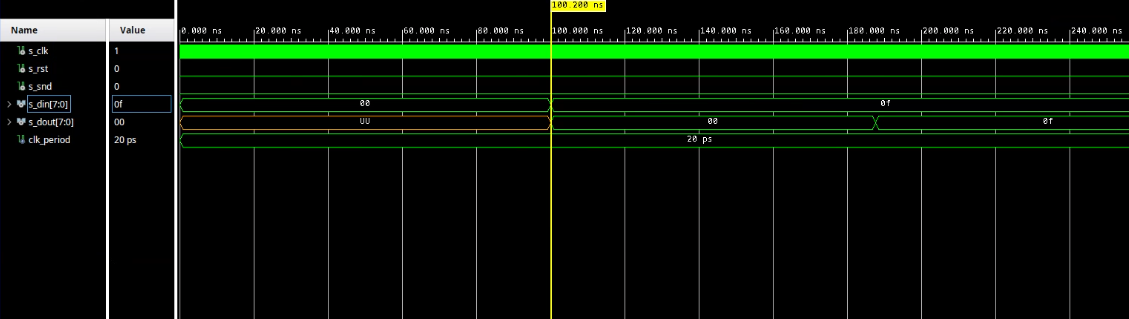
\includegraphics[width=17cm]{immagini/esercizio9/output_simulazione_9.1.png}
    \caption{Simulazione 9.1}
    \label{fig:my_label}
\end{figure}

\subsection{Sintesi su scheda}
Per implementare il sistema sulla scheda sono stati innanzitutto utilizzati i componenti \textit{button\_debouncer} per gestire gli input dei pulsanti. L'uscita del sistema AB è stata mappata con i led appropriati tramite il file dei constraint.
La modifica principale che è stata apportata riguarda la modifica del clock, che ha particolare incidenza sulla periferica seriale.
La UART è stata infatti impostata con \textit{baud rate} e \textit{baud divide} relativi a una frequenza di 48Mhz, mentre il clock di base della scheda ha una frequenza di 100Mhz. 
È stato quindi inserito un divisore di frequenza che la dimezza in output, e fornisce il clock agli altri componenti del sistema.
Nel file video 9.1 è mostrato il funzionamento della scheda, con diverse trasmissioni e reset.

Di seguito è mostrato il codice relativo al componente che ingloba gli altri:

\begin{lstlisting} [language=VHDL, caption=Testing sistema AB]
library IEEE;
use IEEE.STD_LOGIC_1164.ALL;

entity top is
    Port (
        snd, clk, rst: in std_logic;
        din : in std_logic_vector(7 downto 0);
        dout : out std_logic_vector(7 downto 0)
    );

end top;

architecture Behavioral of top is
    component ab is
        Port (
            snd, clk, rst: in std_logic;
            din : in std_logic_vector(7 downto 0);
            dout : out std_logic_vector(7 downto 0)
        );
    end component ab;

    component ButtonDebouncer is
        generic (
            CLK_period: integer := 10;  -- periodo del clock in nanosec
            btn_noise_time: integer := 10000000 --durata dell'oscillazione in nanosec
        );
        Port ( RST : in STD_LOGIC;
             CLK : in STD_LOGIC;
             BTN : in STD_LOGIC;
             CLEARED_BTN : out STD_LOGIC);
    end component ButtonDebouncer;

    component clock_divider is
        generic(
            clock_frequency_in : integer := 100000000;--100MHz
            clock_frequency_out : integer := 50000000 --50MHz
        );
        Port ( clock_in : in STD_LOGIC;
             reset : in STD_LOGIC;
             clock_out : out STD_LOGIC);
    end component;

    signal db1_out,s_clk: std_logic ;

begin

    db1: ButtonDebouncer port map(
            RST => rst,
            CLK => s_clk ,
            BTN => snd,
            CLEARED_BTN => db1_out

        );

    sis_ab: ab port map(
            snd =>db1_out,
            clk => s_clk,
            rst => rst,
            din => din,
            dout => dout
        );

    divisore: clock_divider
        port map(
            clock_in=>clk ,
            reset=>rst,
            clock_out=>s_clk
        );
end Behavioral;
\end{lstlisting}

















\section{UART MEM}
\paragraph{Traccia} Come variante dell’esercizio 9.1, il sistema A invia al sistema B tramite l’interfaccia seriale N stringhe di 8 bit contenute all’interno di una memoria ROM. Le stringhe ricevute vengono memorizzate in una memoria locale a B. Il progetto deve prevedere che A utilizzi un componente contatore per scandire le N stringhe da inviare.

\subsection{Architettura}
Analogamente all'esercizio precedente il sistema è realizzato con un approccio strutturale. Sono stati aggiunti una serie di componenti per implementare le nuove funzionalità.

Il sistema A è composto da:
\begin{itemize}
    \item \textit{UART}: il componente, fornitoci a priori, costituisce in un'interfaccia per la trasmissione del dato tra i due sistemi;
    \item \textit{rom}: una memoria 4x8 contenente le stringhe da inviare a B;
    \item \textit{contatore}: conta il numero di trasmissioni dei dati, in modo tale da terminare opportunamente lo scambio di messaggi; 
    \item \textit{rete di controllo}: regola che la trasmissione dei dati avvenga in modo corretto.
\end{itemize}

Il sistema B, invece, è composto da:
\begin{itemize}
    \item \textit{UART}: il componente, fornitoci a priori, costituisce in un'interfaccia per la trasmissione del dato tra i due sistemi;
    \item \textit{contatore}: conta il numero di ricezioni dei dati, in modo tale da terminare opportunamente lo scambio di messaggi;
    \item \textit{registro}: registro in cui si è scelto di memorizzare temporaneamente la stringa trasmessa da A;
    \item \textit{memoria}: memoria interna a B, dove vengono memorizzate le stringhe ricevute da A;
    \item \textit{rete di controllo}: regola che la trasmissione e l'output dei dati avvenga in modo corretto.
\end{itemize}

Le interconnessioni tra i due sistemi sono visibili nella seguente architettura: 
\begin{figure}[H]
    \centering
    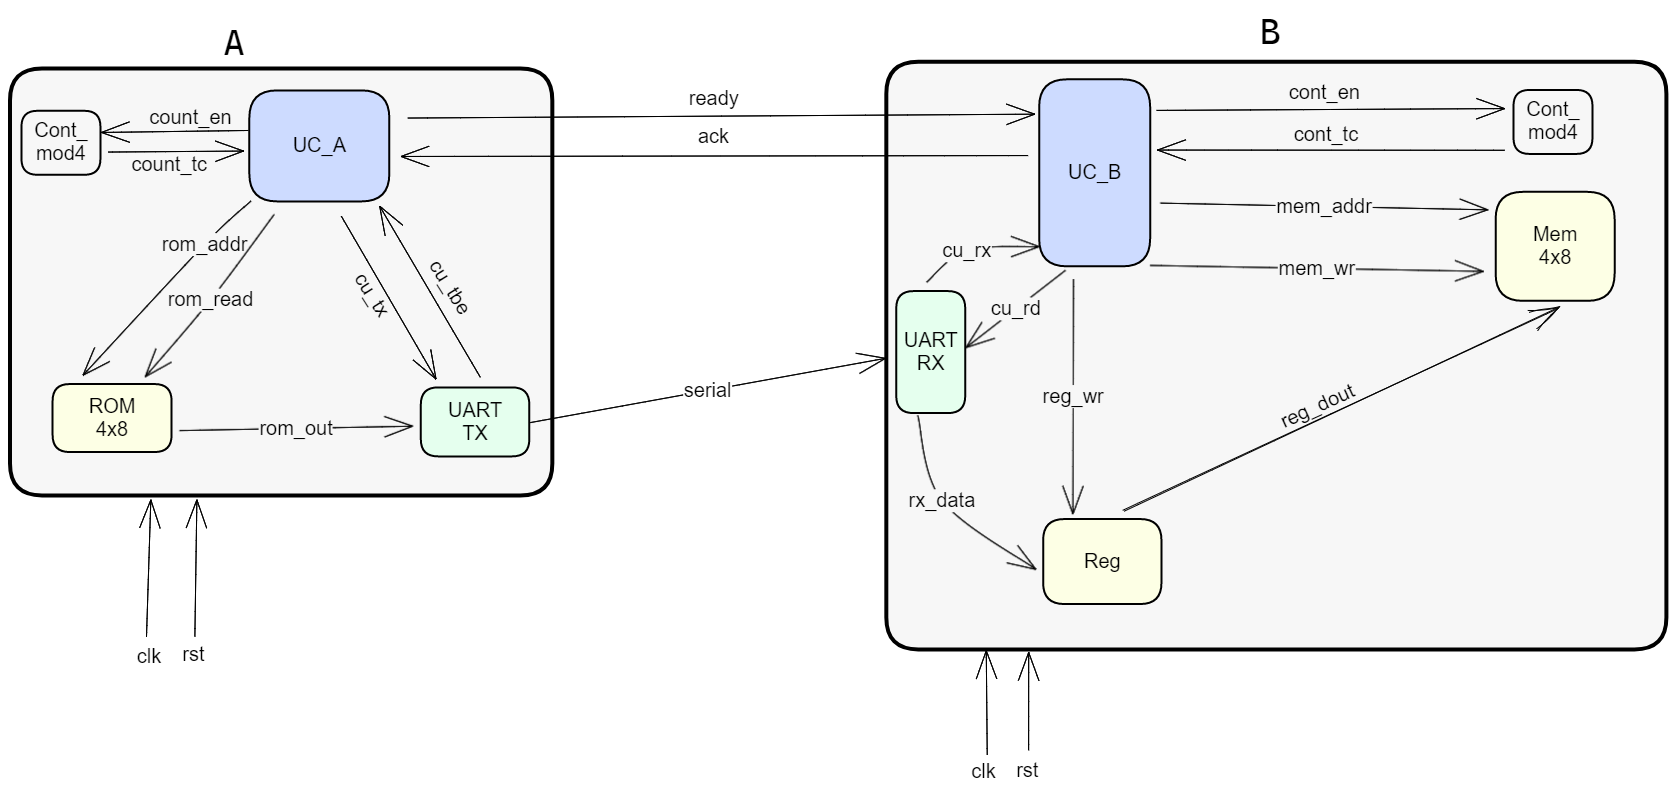
\includegraphics[width=17cm]{immagini/esercizio9/schema_9.2.png}
    \caption{Schema Interfaccia Seriale}
    \label{fig:my_label}
\end{figure}

Gli automi di A e B si occupano di gestire i componenti delle architetture e comunicano tra loro con un semplice \textit{two-way handshake}, con i segnali ready ed ack come descritto nei capitoli precedenti. 
Le differenze principali rispetto all'esercizio precedente stanno nell'assenza del segnale \textit{done}, che indicava ad A la fine della trasmissione, e la necessita di scrivere o leggere dalle memorie interne dei dispositivi incrementando mano mano l'indirizzo.

Nell'automa A oltre al normale autociclo che deve aspettare l'ack alto prima di trasmettere sono stati aggiunti altre due condizioni di \textit{wait} per sincronizzare la comunicazione:
la prima aspetta che il segnale della UART \textit{tbe} sia alto , che indica la fine dell'invio dei dati, e la seconda aspetta che l'ack di B si abbassi, in modo da essere sicuri di non finire e ritrovarlo ancora alto mentre B sta finendo di ricevere, facendo partire una trasmissione errata. La gestione dell'indirizzo per scrivere in memoria e il contatore per scandire il numero di trasmissioni è omologa a quella vista nell'esercizio 7, per cui arrivati al numero massimo si arriverà nello stato idle.

L'automa B ha subito meno variazioni rispetto ad A, ci sono due auto-cicli per aspettare il segnale di \textit{ready} alto e per aspettare il segnale \textit{RDA} della UART, in modo da poter alzare il segnale di lettura dalla seriale, scrivere il valore in un registro temporaneo, e poi scrivere in memoria il risultato alla locazione giusta.
L'utilizzo del registro temporaneo permette ai componenti delle seriali di riprendere il prima possibile la comunicazione senza impattare sul dato già arrivato, che in contemporanea sta venendo scritto in memoria. Se l'uscita del ricevitore fosse stata collegata direttamente alla memoria ci sarebbe stato il rischio di un cambio del dato.

Di seguito è possibile osservare la stesura degli automi dei singoli sistemi: 
\begin{figure}[H]
    \centering
    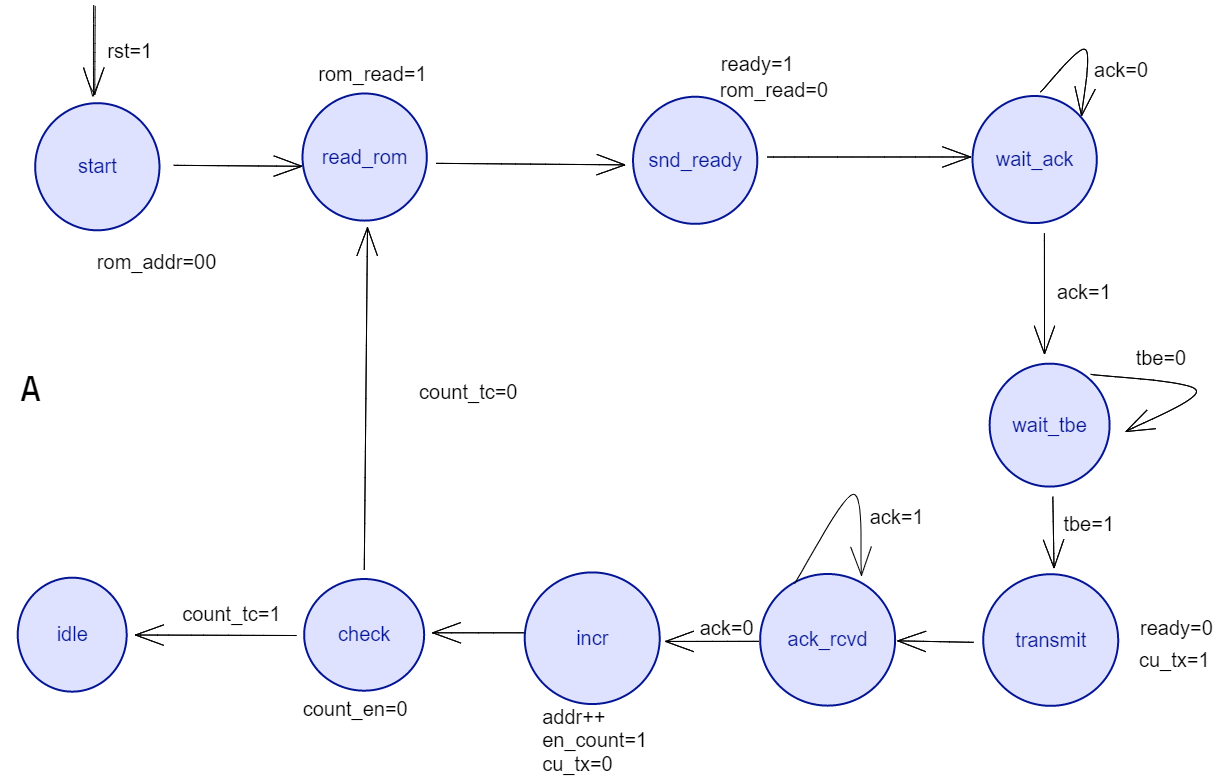
\includegraphics[width=17cm]{immagini/esercizio9/automaA_9.2.png}
    \caption{Automa A}
    \label{fig:my_label}
\end{figure}

\begin{figure}[H]
    \centering
    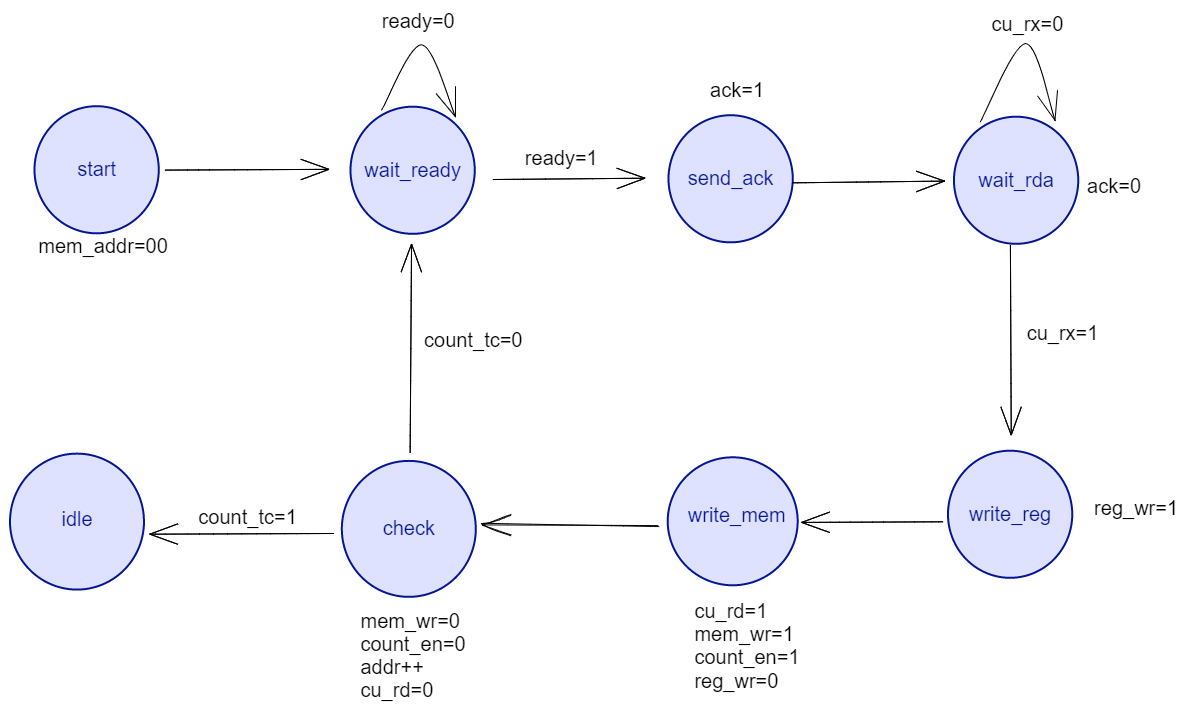
\includegraphics[width=17cm]{immagini/esercizio9/automaB_9.2.png}
    \caption{Automa B}
    \label{fig:my_label}
\end{figure}


Di seguito il codice di A e B:
N.B.: per semplicità è stato omesso il codice della UART.
\begin{lstlisting} [language=VHDL, caption=Contatore mod4]
library IEEE;
use IEEE.std_logic_1164.all;
use IEEE.numeric_std.all;

entity cont_mod4 is
    port (
        clk, rst: in std_logic;
        tc: out std_logic
    );
end entity cont_mod4;

architecture rtl of cont_mod4 is
    signal count: std_logic_vector(1 downto 0) := "00";
begin
    cont: process(clk)
    begin
        if rising_edge(clk) then
            if rst = '1' then
                count <="00";
                tc <= '0';
            elsif count = "11" then
                tc <= '1';
                count <= (others => '0');
            else 
                 tc <= '0';
                 count <= std_logic_vector((unsigned(count) + 1));
               
            end if;
        end if;
   end process cont;
    
end architecture rtl;
\end{lstlisting}

\begin{lstlisting} [language=VHDL, caption=Rete di controllo di A]
library IEEE;
use IEEE.STD_LOGIC_1164.ALL;
use IEEE.numeric_std.all;

entity cu_a is
    port(
        clk, rst, ack, count_tc, cu_tbe: in std_logic;
        ready, cu_tx, rom_read, count_en: out std_logic;
        rom_addr: out std_logic_vector(1 downto 0)
    );
end cu_a;

architecture behavioral of cu_a is

    type state is (
        START,
        READ_ROM,
        SND_READY,
        WAIT_ACK,
        WAIT_TBE,
        TRANSMIT,
        ACK_RCVD,
        INCR,   
        CHECK,
        IDLE
    );
    signal current_state : state:= IDLE;
    signal next_state : state;
    signal s_addr: std_logic_vector(1 downto 0) := "00";

begin
    comb: process(current_state, ack, cu_tbe)
    begin
        case current_state is

            when START =>
                ready <= '0';
                s_addr <= "00";
                rom_read <= '0';
                cu_tx <= '0';
                count_en <= '0';
                next_state<= READ_ROM;

            when READ_ROM=>
                rom_read <= '1';
                next_state <= SND_READY;

            when SND_READY=>
                rom_read <= '0';
                ready <= '1';
                next_state <= WAIT_ACK;

            when WAIT_ACK=>
                if ( ack = '1' ) then
                    next_state <= WAIT_TBE;
                else
                    next_state <= WAIT_ACK;
                end if;

            when WAIT_TBE =>
                if cu_tbe = '1' then
                    next_state <= TRANSMIT;
                else
                    next_state <= WAIT_TBE;
                end if;

            when TRANSMIT=>
                cu_tx <= '1';
                ready <= '0';
                next_state <= ACK_RCVD;
                
            when ACK_RCVD => 
                if ack = '0' then
                    next_state <=  INCR;
                else 
                    next_state <= ACK_RCVD;
                end if;

           when INCR =>
                cu_tx <= '0';
                s_addr <= std_logic_vector((unsigned(s_addr) + 1));
                count_en <= '1';
                next_state <= CHECK;
    
            when CHECK =>
                count_en <= '0';
                if count_tc = '1' then
                    next_state <= IDLE;
                else
                    next_state <= READ_ROM;
                end if;

            when IDLE=>
                next_state<= IDLE;
            when others => next_state<= IDLE;
        end case;
    end process comb;

    rom_addr <= s_addr;

    seq: process(clk)
    begin
        if rising_edge(clk) then
            if rst='1'  then
                current_state<=START;
            else
                current_state<=next_state;
            end if;
        end if;
    end process seq;
end behavioral;
\end{lstlisting}

\begin{lstlisting} [language=VHDL, caption=Rom di A]
library ieee;
use ieee.std_logic_1164.all;
use ieee.numeric_std.all;

entity rom_a is
port(
    clk, read : in std_logic; 
    addr : in std_logic_vector(1 downto 0);
    data : out std_logic_vector(7 downto 0)
    );
end rom_a;

architecture behavioral of rom_a is 
type rom_t is array (0 to 3) of std_logic_vector(7 downto 0);
signal rom : rom_t := (
    "00000010", 
    "00000110", 
    "00001001", 
    "00001111"
);

begin

process(clk)
  begin
    if rising_edge(clk) then
        if read = '1' then
            data <= rom(to_integer(unsigned(addr)));
        end if;
    end if;
end process;
end behavioral;
\end{lstlisting}

Di seguito il codice di A:
\begin{lstlisting} [language=VHDL, caption=Sistema A]
library IEEE;
use IEEE.STD_LOGIC_1164.ALL;

entity a is
    Port (
        clk, ack, rst: in std_logic ;
        ready, data: out std_logic
    );
end a;

architecture Structural of a is

    component cont_mod4 is
        port (
            clk, rst: in std_logic;
            tc: out std_logic
        );
    end component cont_mod4;

    component cu_a is
        port(
            clk, rst, ack, count_tc, cu_tbe: in std_logic;
            ready, cu_tx, rom_read, count_en : out std_logic;
            rom_addr: out std_logic_vector(1 downto 0)
        );
    end component cu_a;


    component rom_a is
        port(
            clk, read : in std_logic;
            addr : in std_logic_vector(1 downto 0);
            data : out std_logic_vector(7 downto 0)
        );
    end component rom_a;

    component UARTcomponent is
        Generic (
            --@48MHz
            --		BAUD_DIVIDE_G : integer := 26; 	--115200 baud
            --		BAUD_RATE_G   : integer := 417

            --@26.6MHz
            BAUD_DIVIDE_G : integer := 14; 	--115200 baud
            BAUD_RATE_G   : integer := 231
        );
        Port (
            TXD 	: out 	std_logic  	:= '1';					-- Transmitted serial data output
            RXD 	: in  	std_logic;							-- Received serial data input
            CLK 	: in  	std_logic;							-- Clock signal
            DBIN 	: in  	std_logic_vector (7 downto 0);		-- Input parallel data to be transmitted
            DBOUT 	: out 	std_logic_vector (7 downto 0);		-- Recevived parallel data output
            RDA		: inout  std_logic;							-- Read Data Available
            TBE		: out 	std_logic 	:= '1';					-- Transfer Buffer Emty
            RD		: in  	std_logic;							-- Read Strobe
            WR		: in  	std_logic;							-- Write Strobe
            PE		: out 	std_logic;							-- Parity error		
            FE		: out 	std_logic;							-- Frame error
            OE		: out 	std_logic;							-- Overwrite error
            RST		: in  	std_logic	:= '0');				-- Reset signal

    end component  UARTcomponent;

    signal count_en, count_tc, rom_read, cu_tx, cu_tbe: std_logic := '0';
    signal rom_addr: std_logic_vector(1 downto 0) := "00";
    signal rom_out: std_logic_vector(7 downto 0) := "00000000";

begin

    cont : cont_mod4
        port map(
            clk=>count_en,
            rst=>rst,
            tc=>count_tc
        );

    cu : cu_a
        port map(
            clk=>clk,
            rst=>rst,
            count_tc=>count_tc ,
            count_en => count_en,
            rom_addr=>rom_addr,
            rom_read=>rom_read,
            ready=>ready,
            ack=>ack,
            cu_tx => cu_tx,
            cu_tbe=>cu_tbe
        );

    rom : rom_a
        port map(
            clk=>clk,
            read=>rom_read,
            addr=>rom_addr,
            data=>rom_out
        );

    uart:  UARTcomponent generic map(
            BAUD_DIVIDE_G=>26,
            BAUD_RATE_G=>417
        )
        port map (
            TXD => data,
            RXD => '1',
            CLK => clk,
            DBIN => rom_out,
            DBOUT => OPEN,
            RDA => OPEN,
            TBE => cu_tbe,
            RD => '0',
            WR => cu_tx,
            PE => OPEN,
            FE => OPEN,
            OE => OPEN,
            RST => rst
        );

end Structural;

\end{lstlisting}


N.B.: il codice del contatore mod4 coincide con il codice del contatore del sistema A e per semplicità è stato omesso il codice della UART.
\begin{lstlisting} [language=VHDL, caption=Registro di B]
library IEEE;
use IEEE.STD_LOGIC_1164.ALL;

entity reg is
    port (
        d: in std_logic_vector (7 downto 0);
        clk, rst: in std_logic ;
        write: in std_logic ;
        q:out std_logic_vector (7 downto 0));
end reg;

architecture Behavioral of reg is

begin
    process (clk)
    begin
        if rising_edge (clk) then
            if (rst='1') then
                q<="00000000";
            elsif(write='1') then
                q<=d;
            end if;
        end if;
    end process;

end Behavioral;

\end{lstlisting}

\begin{lstlisting} [language=VHDL, caption=Memoria di B]
library ieee;
use ieee.std_logic_1164.all;
use ieee.numeric_std.all;

entity memory is
    port(
        clk, write, rst : in std_logic;
        addr : in std_logic_vector(1 downto 0);
        input : in std_logic_vector(7 downto 0);
        output : out std_logic_vector(7 downto 0)
    );
end memory;

architecture behavioral of memory is
    type mem_t is array (0 to 3) of std_logic_vector(7 downto 0);
    signal mem : mem_t := (
        "00000000",
        "00000000",
        "00000000",
        "00000000"
    );

begin
    process(clk)
    begin
        if rising_edge(clk) then
            if rst = '1' then
                for i in 0 to 3 loop
                    mem(i) <= "00000000";
                end loop;
            elsif write = '1' then
                mem(to_integer(unsigned(addr))) <= input;
            end if;
        end if;
        output<=mem(to_integer(unsigned(addr)));
    end process;
end behavioral;
\end{lstlisting}

\begin{lstlisting} [language=VHDL, caption=Rete di controllo di B]
library IEEE;
use IEEE.STD_LOGIC_1164.ALL;
use IEEE.numeric_std.all;

entity cu_b is
    port(
        clk, rst, ready,  count_tc, cu_rx: in std_logic;
        ack, count_en, reg_wr, mem_wr, cu_rd: out std_logic;
        mem_addr: out std_logic_vector(1 downto 0)
    );
end cu_b;

architecture behavioral of cu_b is

    type state is (
        START,
        WAIT_READY,
        SEND_ACK,
        WAIT_RDA,
        WRITE_REG,
        WRITE_MEM,
        CHECK,
        IDLE
    );
    signal current_state : state:= IDLE;
    signal next_state : state;
    signal s_addr: std_logic_vector(1 downto 0) :=(others => '0');

begin
    comb: process(current_state, ready, cu_rx)
        variable somma: unsigned(8 downto 0) := (others => '0');
    begin
        case current_state is

            when START =>
                ack <= '0';
                s_addr <= "00";
                count_en <= '0';
                cu_rd <= '0';
                mem_wr <= '0';
                reg_wr <= '0';
                next_state<= WAIT_READY;

            when WAIT_READY=>
                if ( ready = '1' ) then
                    next_state <= SEND_ACK;
                else
                    next_state <= WAIT_READY;
                end if;

            when SEND_ACK=>
                ack <= '1';
                next_state <= WAIT_RDA;

            when WAIT_RDA=>
                ack <= '0';
                if ( cu_rx = '1' ) then
                    next_state <= WRITE_REG;
                else
                    next_state <= WAIT_RDA;
                end if;

            when WRITE_REG=>
                reg_wr <= '1';
                next_state <= WRITE_MEM;

            when WRITE_MEM=>
                cu_rd <= '1';
                mem_wr <= '1';
                count_en <= '1';
                reg_wr <= '0';
                next_state <= CHECK;

            when CHECK =>
                mem_wr <= '0';
                cu_rd <= '0';
                count_en <= '0';
                s_addr <= std_logic_vector((unsigned(s_addr) + 1));
                
                if count_tc = '1' then
                    next_state <= IDLE;
                else
                    next_state <= WAIT_READY;
                end if;

            when IDLE=>
                next_state<= IDLE;
            when others => next_state<= IDLE;
        end case;
    end process comb;

    mem_addr <= s_addr;

    seq: process(clk)
    begin
        if rising_edge(clk) then
            if rst='1'  then
                current_state<=START;
            else
                current_state<=next_state;
            end if;
        end if;
    end process seq;
end behavioral;
\end{lstlisting}

\begin{lstlisting} [language=VHDL, caption=Sistema B]
library IEEE;
use IEEE.STD_LOGIC_1164.ALL;

entity b is
    Port (
        clk, ready, rst, serial_in: in std_logic ;
        ack: out std_logic
    );
end b;

architecture Structural of b is

    component cont_mod4 is
        port (
            clk, rst: in std_logic;
            tc: out std_logic
        );
    end component cont_mod4;

    component reg is
        port (
            d: in std_logic_vector (7 downto 0);
            clk, rst: in std_logic ;
            write: in std_logic ;
            q:out std_logic_vector (7 downto 0));
    end component reg;

    component cu_b is
        port(
            clk, rst, ready,  count_tc, cu_rx: in std_logic;
            ack, count_en, reg_wr, mem_wr, cu_rd: out std_logic;
            mem_addr: out std_logic_vector(1 downto 0)
        );
    end component cu_b;

    component memory is
        port(
            clk, write, rst : in std_logic;
            addr : in std_logic_vector(1 downto 0);
            input : in std_logic_vector(7 downto 0);
            output : out std_logic_vector(7 downto 0)
        );
    end  component memory;

    component UARTcomponent is
        Generic (
            --@48MHz
            --		BAUD_DIVIDE_G : integer := 26; 	--115200 baud
            --		BAUD_RATE_G   : integer := 417

            --@26.6MHz
            BAUD_DIVIDE_G : integer := 14; 	--115200 baud
            BAUD_RATE_G   : integer := 231
        );
        Port (
            TXD 	: out 	std_logic  	:= '1';					-- Transmitted serial data output
            RXD 	: in  	std_logic;							-- Received serial data input
            CLK 	: in  	std_logic;							-- Clock signal
            DBIN 	: in  	std_logic_vector (7 downto 0);		-- Input parallel data to be transmitted
            DBOUT 	: out 	std_logic_vector (7 downto 0);		-- Recevived parallel data output
            RDA		: inout  std_logic;							-- Read Data Available
            TBE		: out 	std_logic 	:= '1';					-- Transfer Buffer Emty
            RD		: in  	std_logic;							-- Read Strobe
            WR		: in  	std_logic;							-- Write Strobe
            PE		: out 	std_logic;							-- Parity error		
            FE		: out 	std_logic;							-- Frame error
            OE		: out 	std_logic;							-- Overwrite error
            RST		: in  	std_logic	:= '0');				-- Reset signal

    end component  UARTcomponent;

    signal count_en, count_tc, cu_rx, cu_rd, mem_wr, reg_wr: std_logic := '0';
    signal mem_addr: std_logic_vector(1 downto 0) := "00";
    signal rx_data, reg_dout: std_logic_vector(7 downto 0) := "00000000";

begin

    cont : cont_mod4
        port map(
            clk=>count_en,
            rst=>rst,
            tc=>count_tc
        );

    reg_b: reg
        port map(
            clk=> clk,
            rst=>rst,
            write=>reg_wr,
            d=>rx_data,
            q=>reg_dout
        );

    cu : cu_b
        port map(
            clk=>clk,
            rst=>rst,
            count_tc=>count_tc ,
            count_en => count_en,
            mem_addr=>mem_addr,
            mem_wr => mem_wr,
            reg_wr => reg_wr,
            ready=>ready,
            ack=>ack,
            cu_rx => cu_rx,
            cu_rd => cu_rd
        );


    mem: memory 
        port map(
            clk=>clk,
            rst=>rst,
            write => mem_wr,
            addr=>mem_addr,
            input=>reg_dout,
            output=>OPEN
        );
 
    uart:  UARTcomponent generic map(
            BAUD_DIVIDE_G=>26,
            BAUD_RATE_G=>417
        )
        port map (
            TXD => OPEN,
            RXD => serial_in,
            CLK => clk,
            DBIN => "00000000",
            DBOUT => rx_data,
            RDA => cu_rx,
            TBE => OPEN,
            RD => cu_rd,
            WR => '0',
            PE => OPEN,
            FE => OPEN,
            OE => OPEN,
            RST => rst
        );

end Structural;

\end{lstlisting}

Infine, è possibile osservare il codice dell'intero sistema AB:
\begin{lstlisting} [language=VHDL, caption=Sistema AB]
library IEEE;
use IEEE.STD_LOGIC_1164.ALL;

entity ab is
 Port (
    clk, rst: in std_logic
  );
end ab;

architecture Structural of ab is

component a is
    Port (
        clk, ack, rst: in std_logic ;
        ready, data: out std_logic
    );
end component a;

component b is
    Port (
        clk, ready, rst, serial_in: in std_logic ;
        ack: out std_logic
    );
end component b;

signal ack, ready, data: std_logic := '0';

begin
    UnitA: a port map(
        clk=>clk,
        rst=>rst,
        ready=>ready,
        ack=>ack,
        data=>data
       );

    UnitB: b port map(
        clk=>clk,
        rst=>rst,
        ready=>ready,
        ack=>ack,
        serial_in=>data
       );


end Structural;

\end{lstlisting}

\subsection{Simulazione}
Per una maggiore sicurezza si è scelto di testare prima la rete di controllo del sistema A singolarmente e poi di effettuare la simulazione dell'intero sistema di Interfaccia Seriale.

\begin{figure}[H]
    \centering
    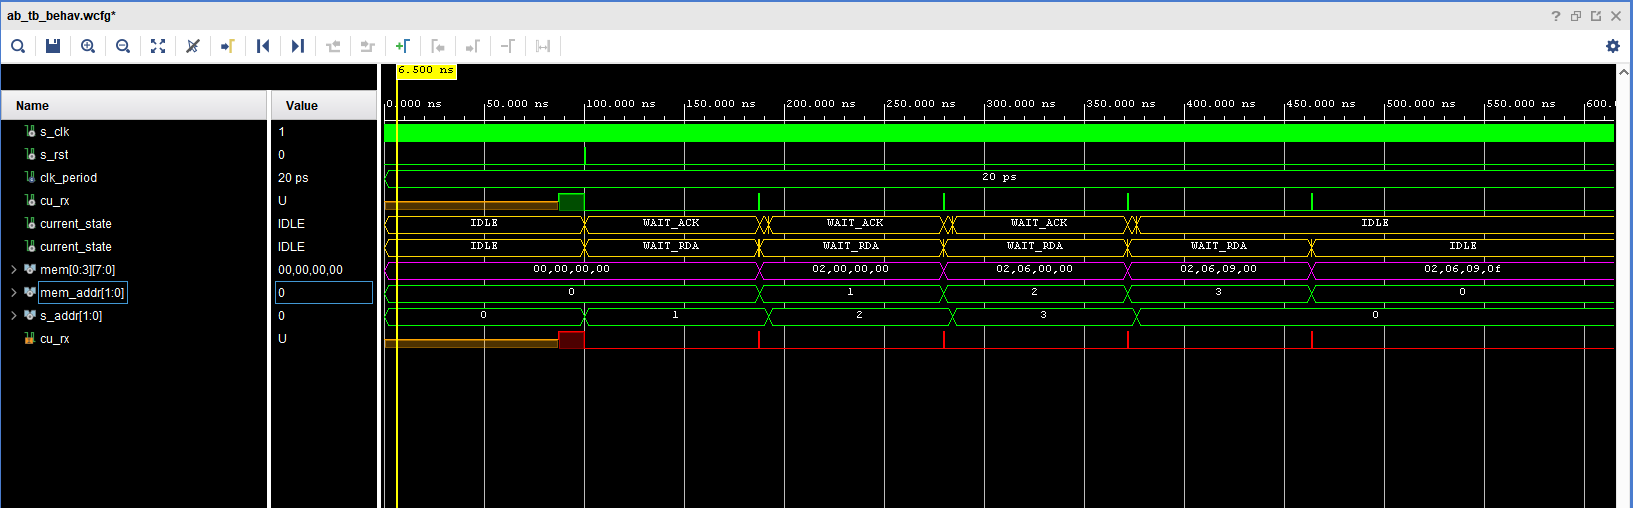
\includegraphics[width=17cm]{immagini/esercizio9/simulazione_9.2.png}
    \caption{Simulazione AB}
    \label{fig:sim_9.2}
\end{figure}


\paragraph{Testbench}

\begin{lstlisting} [language=VHDL, caption=Testing rete di controllo di A]
library IEEE;
use IEEE.STD_LOGIC_1164.ALL;

entity cu_a_tb is
end cu_a_tb;

architecture Behavioral of cu_a_tb is

    component cu_a is
        port(
            clk, rst, ack, done, count_tc: in std_logic;
            ready, cu_tx, rom_read, count_en : out std_logic;
            rom_addr: out std_logic_vector(1 downto 0)
        );
    end component cu_a;

    signal s_clk, s_rst, s_count_tc, s_count_en, s_ready, s_done, s_ack, s_cu_tx, s_rom_read: std_logic := '0';
    signal s_rom_addr : std_logic_vector(1 downto 0) := "00";
    constant clk_period:time := 10ns;

begin

    uut : cu_a
        port map(
            clk=>s_clk,
            rst=>s_rst,
            count_tc=>s_count_tc ,
            count_en => s_count_en,
            rom_addr=>s_rom_addr,
            rom_read=>s_rom_read,
            ready=>s_ready,
            done => s_done,
            ack=>s_ack,
            cu_tx => s_cu_tx
        );

    tb: process
    begin
        wait for 100ns;
        s_rst <='1';
        wait for clk_period;
        s_rst <='0';

        wait until s_ready = '1';
        wait for clk_period;
        s_ack <= '1';
        wait for clk_period;
        s_ack <= '0';
        wait for clk_period;
        s_done <= '1';
        wait for clk_period;
        s_done <= '0';
        wait for clk_period;
    
        wait;
    end process tb;

    clock: process
    begin
        loop
            s_clk <= not s_clk;
            wait for clk_period/2;
        end loop;
    end process clock;

end Behavioral;

\end{lstlisting}

\begin{lstlisting} [language=VHDL, caption=Testing sistema AB]
library IEEE;
use IEEE.STD_LOGIC_1164.ALL;

entity ab_tb is
end ab_tb;

architecture Behavioral of ab_tb is

   component ab is port (         
        clk,rst: in std_logic        
  );
    end component ab;

    signal s_clk, s_rst: std_logic := '0';
    constant clk_period: time := 20ps;

begin
    uut: AB port map(
            clk=>s_clk,         
            rst=>s_rst
        );

    tb: process
    begin
        wait for 100ns;
        s_rst <='1';
        wait for clk_period;
        s_rst <='0';
        
        wait;
    end process tb;

    clock: process
    begin
        loop
            s_clk <= not s_clk;
            wait for clk_period/2;
        end loop;
    end process clock;
end Behavioral;
\end{lstlisting}


\chapter{Omega Network}

\section{Omega Network}

Progettare e implementare in VHDL uno switch multistadio secondo il modello omega network. Lo switch deve consentire lo scambio di messaggi di 2 bit ciascuno da un nodo sorgente a un nodo destinazione in una rete con 4 nodi, implementando uno schema a priorità fissa fra i nodi (ed. nodo 1 più prioritario, con priorità decrescenti fino al nodo 4). 

\subsection{Architettura}

L'architettura è costituita da due componenti: un unità operativa e una rete di controllo.

La rete di controllo serve a gestire la priorità tra i nodi, ed è costituita da un multiplexer 4:1, un demultiplexer 1:4 ed un arbitro.
In particolare per poter inviare un dato è necessario alzare un segnale di \textit{enable}, oltre che specificare mittente, destinatario e i bit di contenuto, e l'arbitro della rete di controllo si occupa di gestire eventuale conflitti tra le abilitazioni, dando priorità in maniera statica a i primi (da 0 a 3). In questo modo si evitano possibili collisioni durante il trasferimento dei dati.
La \textit{frame} di 6 bit che entra in input attraverso le porte a0...a3 è strutturata nel seguente modo:

\begin{figure}[H]
    \centering
    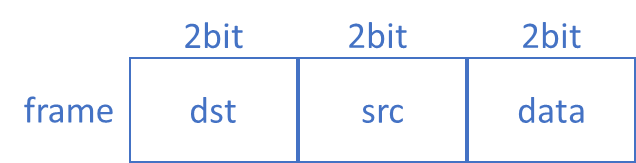
\includegraphics[width=15cm]{immagini/esercizio10/frame_omega.png}
    \caption{Frame Omega Network}
\end{figure}
Gli indirizzi di sorgente e destinazione vengono separati dai dati effettivi. I primi escono sulle omonime uscite, mentre i dati da b0...b3.

L'unità operativa implementa effettivamente il trasferimento del dato da una linea all'altra ed è costituita da un insieme di 4 switch.
Il modo in cui sono connessi questi quattro switch rispetta la definizione di omega nework che sfrutta l’idea del perfect shuffling.
Questa tecnica permette  di ottimizzare i percorsi da seguire indicando i modi di collegamento tra i diversi stadi.

\begin{figure}[H]
    \centering
    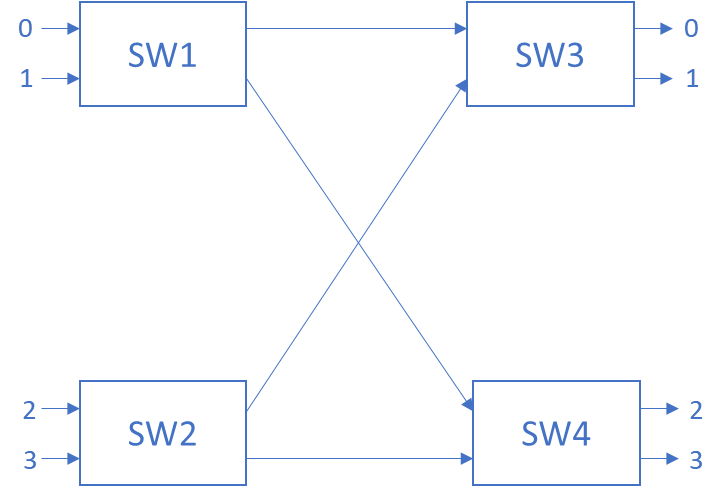
\includegraphics[width=15cm]{immagini/esercizio10/omega2x2.png}
    \caption{Frame Omega Network}
\end{figure}

Per poter determinare il percorso da seguire, una volta collegati gli switch in questa configurazione, basta leggere in ordine i bit della destinazione dal più significativo al meno significativo, e a ogni stadio usare l'uscita superiore se il bit è 0 e la inferiore se il bit è 1. Specularmente, per capire da quale sorgente leggere si leggono i bit di sorgente a partire dal meno significativo.
La comunicazione tra gli switch avviene in modalità combinatoria, e i dettagli implementativi sono mostrati nelle sezioni successive. Nel prossimo esercizio, presente tra quelli a scelta, verrà esplorata la soluzione sequenziale, che prevede un handshake tra gli switch.

\paragraph{Switch}
Lo switch è il componente fondamentale della parte operativa ed è stato progettato sulla base dell'esercizio 1.2. In particolare, è stato implementato uno \textit{switch} \textit{2x2} che collega due sorgenti a due destinazioni partendo da un \textit{multiplexer} 2:1 e un \textit{de-multiplexer} 1:2 controllati rispettivamente dai segnali di sorgente e destinazione. Nel listato\ref{switch}, è mostrata l'implementazione di uno switch. Si noti che in questa prima versione dell'esercizio, lo \textit{switch} è puramente combinatorio.


\begin{lstlisting} [language=VHDL, label=switch, caption=Switch]
library IEEE;
use IEEE.STD_LOGIC_1164.ALL;

entity switch is
  Port (
        src, dst: in std_logic;
        a0, a1: in std_logic_vector(1 downto 0);
        b0, b1: out std_logic_vector(1 downto 0)
   );
end switch;

architecture Structural of switch is

component mux_21 is
    Port (
        a0, a1: in std_logic_vector(1 downto 0);
        s : in std_logic;
        u : out std_logic_vector(1 downto 0)
    );
end component mux_21;

component demux_1_2 is
    port (
        a: in std_logic_vector(1 downto 0);
        s: in std_logic;
        u0, u1: out std_logic_vector(1 downto 0)
    );
end component demux_1_2;

signal s_link: std_logic_vector(1 downto 0);
begin

m: mux_21 port map(
    a0=>a0,
    a1=>a1,
    s => src,
    u=>s_link
);

d: demux_1_2 port map(
    a=>s_link,
    u0=>b0,
    u1 => b1,
    s=>dst
);

end Structural;
\end{lstlisting}

\paragraph{Parte operativa}
La parte operativa è stata creando istanziando 2 stadi, ciascuno composto da 2 switch. In particolare, come mostrato in Figura \ref{fig:uo_omega},al primo livello sono collegati il bit meno significativo dell'indirizzo sorgente e quello più significativo della destinazione, viceversa al secondo livello. Gli \textit{switch}, invece, sono collegati secondo la tecnica del \textit{perfect shuffling} illustrata in precedenza. I segnali di ingresso provengono dalla rete di controllo.
Infine, nel listato \ref{uo_omega}, è riportata l'implementazione con approccio strutturale dell'unità operativa.

\begin{figure}[H]
    \centering
    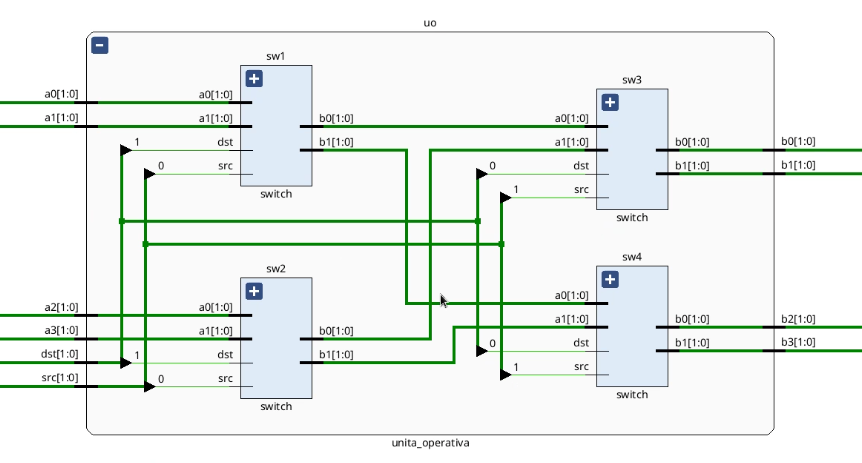
\includegraphics[width=15cm]{immagini/esercizio10/schema_10.1_unitaoperativa.png}
    \caption{Schema unità operativa omega network}
    \label{fig:uo_omega}
\end{figure}


\begin{lstlisting} [language=VHDL,label=uo_omega, caption=Unità operativa]
library IEEE;
use IEEE.STD_LOGIC_1164.ALL;

entity unita_operativa is
  Port (
        a0, a1, a2, a3: in std_logic_vector(1 downto 0);
        src, dst: in std_logic_vector(1 downto 0);
        b0, b1, b2, b3: out std_logic_vector(1 downto 0)
   );
end unita_operativa;

architecture Structural of unita_operativa is

component switch is
  Port (
        src, dst: in std_logic;
        a0, a1: in std_logic_vector(1 downto 0);
        b0, b1: out std_logic_vector(1 downto 0)
   );
end component switch;

signal s_sw1_3, s_sw1_4,  s_sw2_3, s_sw2_4 : std_logic_vector(1 downto 0);

begin
    sw1: switch port map(
        src=>src(0),
        dst=>dst(1),
        a0=> a0,
        a1=> a1,
        b0=> s_sw1_3,
        b1=> s_sw1_4
    );

    sw2: switch port map(
        src=>src(0),
        dst=>dst(1),
        a0=> a2,
        a1=> a3,
        b0=> s_sw2_3,
        b1=> s_sw2_4
    );

    sw3: switch port map(
        src=>src(1),
        dst=>dst(0),
        a0=> s_sw1_3,
        a1=> s_sw2_3,
        b0=> b0,
        b1=> b1
    );

    sw4: switch port map(
        src=>src(1),
        dst=>dst(0),
        a0=> s_sw1_4,
        a1=> s_sw2_4,
        b0=> b2,
        b1=> b3
    );

end Structural;
\end{lstlisting}

\paragraph{Rete di controllo}
La rete di controllo è un componente completamente combinatorio formato da:
\begin{itemize}
    \item multiplexer-demultiplexer: questa rete di trasmissione serve a prendere una frame completa e instradarla nell'uscita corretta dopo aver estratto gli indirizzi di sorgente e destinazione;
    \item arbitro: in questo componente arrivano i segnali di abilitazione degli utenti ($en0...en3$) che vogliono inviare una \textit{frame}. In particolare, è implementato un sistema a priorità che consente di inviare dati in mutua esclusione per evitare conflitti. Le priorità sono assegnate nel seguente modo $pr_3<pr_2<pr_1<pr_0$.
\end{itemize}

La rete di controllo mette in uscita la \textit{frame} da inviare e due segnali che corrispondono agli indirizzi sorgenti e destinazione. Questi segnali vengono dati in ingresso alla parte operativa descritta in precedenza. Infine, è riportata nel listato \ref{rc_omega} l'implementazione con approccio strutturale della rete di controllo.

\begin{lstlisting} [language=VHDL, label=rc_omega,caption=Rete di controllo]
library ieee;
use ieee.std_logic_1164.all;

entity rete_di_controllo is
    port (
        a0, a1, a2, a3: in std_logic_vector(5 downto 0);
        en0, en1, en2, en3: in std_logic;
        b0, b1, b2, b3: out std_logic_vector(1 downto 0);
        src, dst: out std_logic_vector(1 downto 0)
    );
end rete_di_controllo;

architecture Structural of rete_di_controllo is

    component arbitro is
        Port (
            en0,en1,en2,en3: in std_logic;
            u: out std_logic_vector(1 downto 0)
        );
    end component arbitro;

    component mux_4_1 is
        Port ( 
            a0,a1,a2,a3: in std_logic_vector (5 downto 0);
            s: in std_logic_vector (1 downto 0);
            u: out std_logic_vector (5 downto 0)
            );
    end component mux_4_1;

    component demux_14 is
        Port (
            a: in std_logic_vector(1 downto 0);
            s: in std_logic_vector (1 downto 0);
            u0,u1,u2,u3: out std_logic_vector(1 downto 0)
        );
    end component demux_14;

    signal s_sel: std_logic_vector(1 downto 0);
    signal s_m_out: std_logic_vector(5 downto 0);

begin
    A: arbitro port map(
            en0=>en0,
            en1=>en1,
            en2=>en2,
            en3=>en3,
            u=>s_sel
        );
    MUX: mux_4_1 port map(
            a0=>a0,
            a1=>a1,
            a2=>a2,
            a3=>a3,
            s=>s_sel,
            u => s_m_out
        );
    DEMUX: demux_14 port map(
            a=>s_m_out (1 downto 0),
            u0=>b0,
            u1=>b1,
            u2=>b2,
            u3=>b3,
            s=>s_sel
        );
    dst <= s_m_out(5 downto 4);
    src <= s_m_out(3 downto 2);

end Structural;
\end{lstlisting}


\begin{lstlisting} [language=VHDL, caption=arbitro]
library ieee;
use ieee.std_logic_1164.all;

entity arbitro is
    Port (
        en0,en1,en2,en3: in std_logic;
        u: out std_logic_vector(1 downto 0)
    );
end arbitro;

architecture Behavioral of arbitro is

begin
    u <= "00" when en0 = '1' else
         "01" when en1 = '1' else
         "10" when en2 = '1' else
         "11" when en3 = '1' else
         "00";
end Behavioral;
\end{lstlisting}


Di seguito, per completezza è riportata la \textit{omega network} implementata creando l'unità operativa e quella di controllo collegandole opportunamente tra loro.
\begin{lstlisting} [language=VHDL, caption=Omega network 2x2]
library IEEE;
use IEEE.STD_LOGIC_1164.ALL;

entity omega_network is
    Port (
        a0,a1,a2,a3: in std_logic_vector (5 downto 0);
        en0, en1, en2, en3: in std_logic;
        b0,b1,b2,b3: out std_logic_vector (1 downto 0)
    );
end omega_network;

architecture Structural of omega_network is

    component unita_operativa is
        Port (
            a0, a1, a2, a3: in std_logic_vector(1 downto 0);
            src, dst: in std_logic_vector(1 downto 0);
            b0, b1, b2, b3: out std_logic_vector(1 downto 0)
        );
    end component unita_operativa;

    component rete_di_controllo is
        port (
            a0, a1, a2, a3: in std_logic_vector(5 downto 0);
            en0, en1, en2, en3: in std_logic;
            b0, b1, b2, b3: out std_logic_vector(1 downto 0);
            src, dst: out std_logic_vector(1 downto 0)
        );
    end  component rete_di_controllo;

    signal  s_c0, s_c1, s_c2,  s_c3:  std_logic_vector(1 downto 0);
    signal s_src, s_dst :  std_logic_vector(1 downto 0);

begin
    rc: rete_di_controllo port map(
            a0 => a0,
            a1=> a1,
            a2=> a2,
            a3=> a3,
            en0=>en0,
            en1=>en1,
            en2=>en2,
            en3=>en3,
            b0=>s_c0,
            b1=> s_c1,
            b2=>s_c2,
            b3=>s_c3,
            src=>s_src,
            dst=>s_dst
        );
    uo: unita_operativa port map(
            a0 => s_c0,
            a1=> s_c1,
            a2=> s_c2,
            a3=> s_c3,
            src=>s_src,
            dst=>s_dst,
            b0=>b0,
            b1=> b1,
            b2=>b2,
            b3=>b3
        );

end Structural;
\end{lstlisting}

\subsection{Testing}
Per dimostrare il corretto funzionamento dell'intera \textit{omega network} è stata testata prima la rete di controllo (i cui risultati sono mostrati in Figura \ref{fig:sim_rc}) sottoponendola al \textit{testbench} nel listato \ref{tb_rc_omega}.

\begin{lstlisting} [language=VHDL, label=tb_rc_omega,caption=Testbench rete di controllo]
library IEEE;
use IEEE.STD_LOGIC_1164.ALL;

entity rete_di_controllo_tb is
end rete_di_controllo_tb;

architecture Behavioral of rete_di_controllo_tb is

    component rete_di_controllo is
        port (
            a0, a1, a2, a3: in std_logic_vector(5 downto 0);
            en0, en1, en2, en3: in std_logic;
            b0, b1, b2, b3: out std_logic_vector(1 downto 0);
            src, dst: out std_logic_vector(1 downto 0)
        );
    end component rete_di_controllo;

    signal s_a0, s_a1, s_a2, s_a3 :  std_logic_vector(5 downto 0) := (others => '0');
    signal s_b0, s_b1, s_b2, s_b3 :  std_logic_vector(1 downto 0) := (others => '0');
    signal s_en0, s_en1, s_en2, s_en3 :  std_logic := '0';
    signal s_src, s_dst:  std_logic_vector(1 downto 0) := (others => '0');

begin
    uut: rete_di_controllo port map (
            a0 => s_a0,
            a1=> s_a1,
            a2=> s_a2,
            a3=> s_a3,
            en0=>s_en0,
            en1=>s_en1,
            en2=>s_en2,
            en3=>s_en3,
            b0=>s_b0,
            b1=> s_b1,
            b2=>s_b2,
            b3=>s_b3,
            src=>s_src,
            dst=>s_dst
        );
            
        tb: process
            begin
                wait for 100ns;
                s_en2 <= '1';
                wait for 10 ns;
                s_a0 <= "100001";
                s_a2 <= "101001";
                wait;
        end process tb;

end Behavioral;
\end{lstlisting}

\begin{figure}[H]
    \centering
    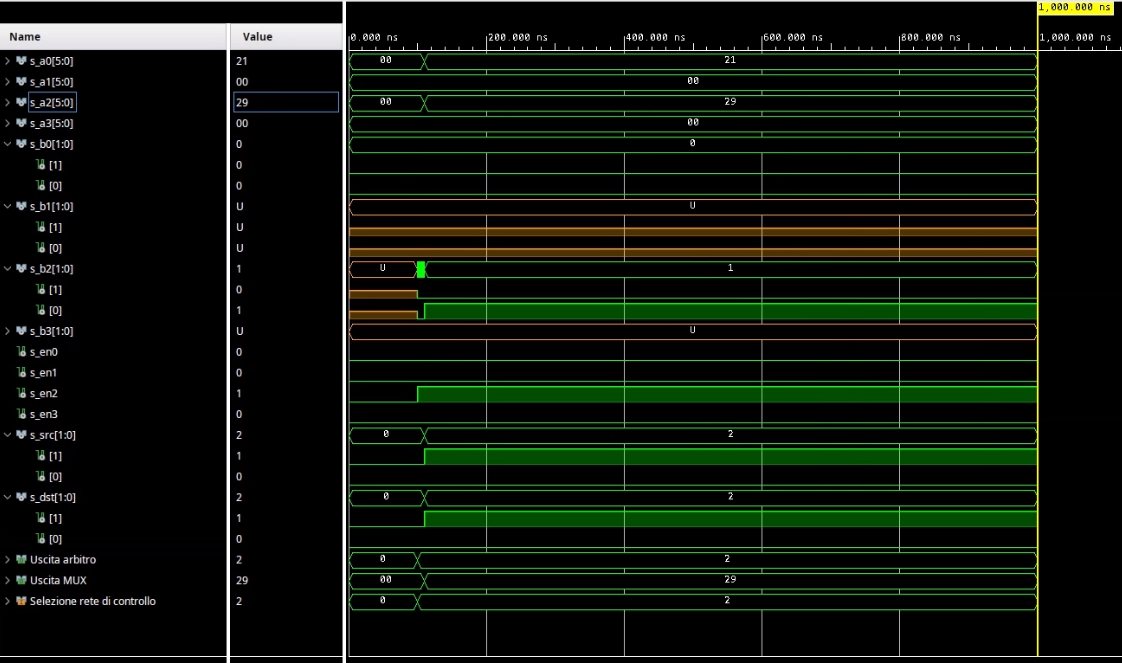
\includegraphics[width=15cm]{immagini/esercizio10/output_simulazione_10.1_retedicontrollo (da vedere se mettere).png}
    \caption{Testing rete di controllo}
    \label{fig:sim_rc}
\end{figure}

Infine, l'\textit{omega network} è stata testata provando ad inviare due \textit{frame}: la prima alzando l'abilitazione dell'utente 2, la seconda l'abilitazione dell'utente 0 (cambiando opportunamente la porta e l'indirizzo sorgente del dato). Si nota che monitorando le uscite destinatarie del pacchetto queste diventano uguali ai due bit meno significativi del \textit{frame}, come illustrato in Figura \ref{fig:sim_on}. Infine, il \textit{testbench} è illustrato nel listato che segue.

\begin{lstlisting} [language=VHDL, label=tbc_omega,caption=Testbench Omega Network]
library IEEE;
use IEEE.STD_LOGIC_1164.ALL;

entity omega_network_tb is
end omega_network_tb;

architecture Behavioral of omega_network_tb is
    component omega_network is
        Port (
            a0,a1,a2,a3: in std_logic_vector (5 downto 0);
            en0, en1, en2, en3: in std_logic;
            b0,b1,b2,b3: out std_logic_vector (1 downto 0)
        );
    end component omega_network;
    signal s_a0, s_a1, s_a2, s_a3 :  std_logic_vector(5 downto 0) := (others => '0');
    signal s_b0, s_b1, s_b2, s_b3 :  std_logic_vector(1 downto 0) := (others => '0');
    signal s_en0, s_en1, s_en2, s_en3 :  std_logic := '0';

begin
    uut: omega_network port map(
            a0 => s_a0,
            a1=> s_a1,
            a2=> s_a2,
            a3=> s_a3,
            en0=>s_en0,
            en1=>s_en1,
            en2=>s_en2,
            en3=>s_en3,
            b0=>s_b0,
            b1=> s_b1,
            b2=>s_b2,
            b3=>s_b3
        );
    process
    begin
        wait for 100ns;
        s_en2 <= '1';
        wait for 10 ns;
        s_a2 <= "101001";
        wait for 10 ns;
        assert (s_b2 = "01") report "Errore riga 44"; 
        wait for 40 ns;
        s_en0 <= '1';
        s_a0 <= "010011";
        wait for 10ns;
        assert (s_b1 = "11") report "Errore riga 48"; 
        wait;
    end process;

end Behavioral;
\end{lstlisting}


\begin{figure}[H]
    \centering
    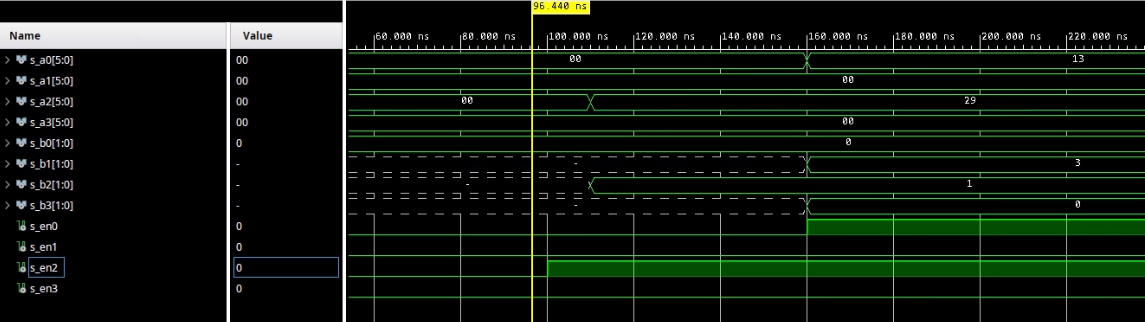
\includegraphics[width=15cm]{immagini/esercizio10/output_simulazione_10.1_omeganetwork.png}
    \caption{Testing Omega Network}
    \label{fig:sim_on}
\end{figure}

\section{Omega Network e Handshaking}
Progettare e implementare in VHDL uno switch multistadio secondo il modello omega network. 
Come punto opzionale si è scelto il punto c:
Si implementi un protocollo di handshaking semplice regolato da una coppia di segnali (pronto a inviare/pronto a ricevere) per l’invio di ciascun messaggio fra due nodi.  

\subsection{Architettura}
L'architettura di base della soluzione è simile a quella precedente. In particolare, l'introduzione della componente sincrona nei requisiti comporta una ri-progettazione della sola parte operativa (\textit{switch}) che deve essere consapevole dei dati trasmessi e ricevuti. Questa funzionalità è stata implementata aggiungendo negli \textit{switch} una rete di controllo implementata con automa a stati finiti.
Per permettere agli \textit{switch} di comunicare tramite un \textit{two-way handshake} è stata inserita al loro interno una piccola unità di controllo che si occupa di gestire i segnali di \textit{ack} e \textit{ready}. L'automa è lo stesso all'interno di tutti gli \textit{switch}, per cui è possibile istanziarne un numero a scelta senza dover effettuare modifiche. Questo rende la soluzione altamente scalabile e più facilmente testabile.
Proprio perché la comunicazione con lo \textit{switch} avviene con un \textit{handshake} sia in entrata che in uscita, anche gli utenti esterni dovranno rispettare il protocollo inviando i segnali di \textit{ack} e \textit{ready} opportunamente, quindi abbiamo un leggero aumento della grandezza della frame. 

Di seguito è mostrato l'automa della rete di controllo dello \textit{switch}:
\begin{figure}[H]
    \centering
    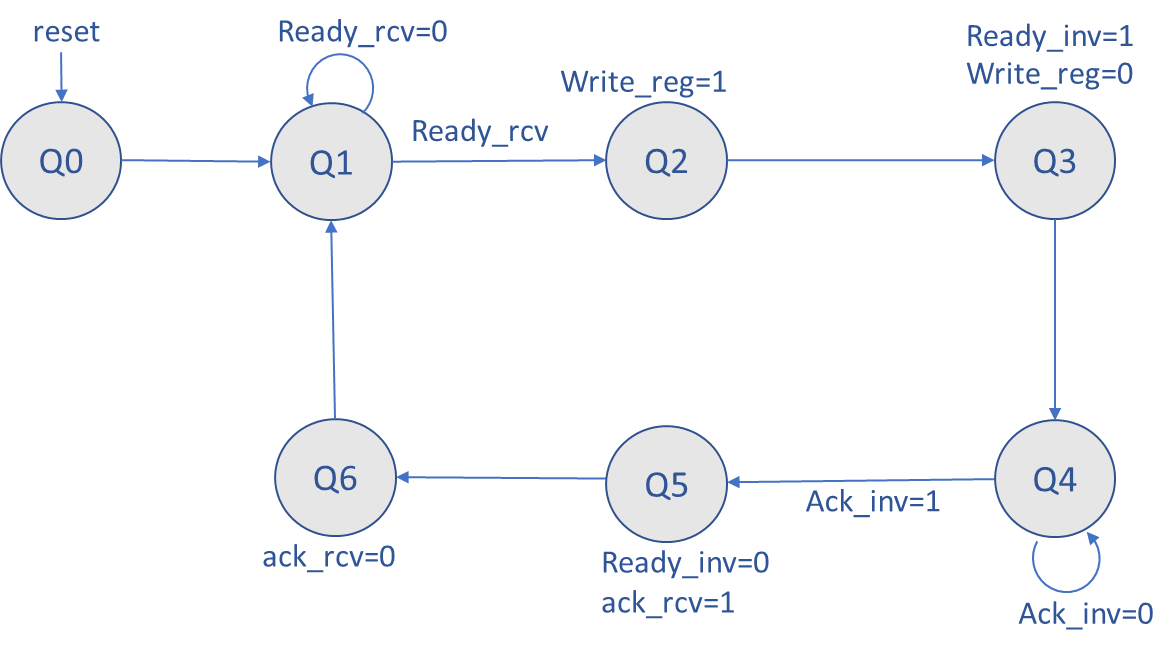
\includegraphics[width=17cm]{immagini/esercizio10/automa_10.3.png}
    \caption{Automa dello \textit{switch}}
    \label{fig:sim_rc}
\end{figure}

Come negli esercizi precedenti si aspettano i segnali di \textit{ready} e \textit{ack} per sincronizzare la comunicazione, ma invece di avere due automi separati ogni automa ha il compito di ricevere e inviare. Questo ha comportato il raddoppio dei segnali di \textit{ack} e \textit{ready}, infatti ci saranno quelli adibiti alla comunicazione con lo stadio precedente e quelli per lo stadio successivo. È stato inoltre aggiunto un semplice registro in uscita allo \textit{switch} poiché il dato non deve cambiare fino a che non arriva l'ack del destinatario.

Per semplicità negli schemi precedenti è stato mostrato l'automa e i segnali relativi a una sola uscita dello \textit{switch}, ma visto che ci sono due ingressi e due uscite tutti i segnali saranno raddoppiati, come mostrato nel seguente schema dell'architettura.

\begin{figure}[H]
    \centering
    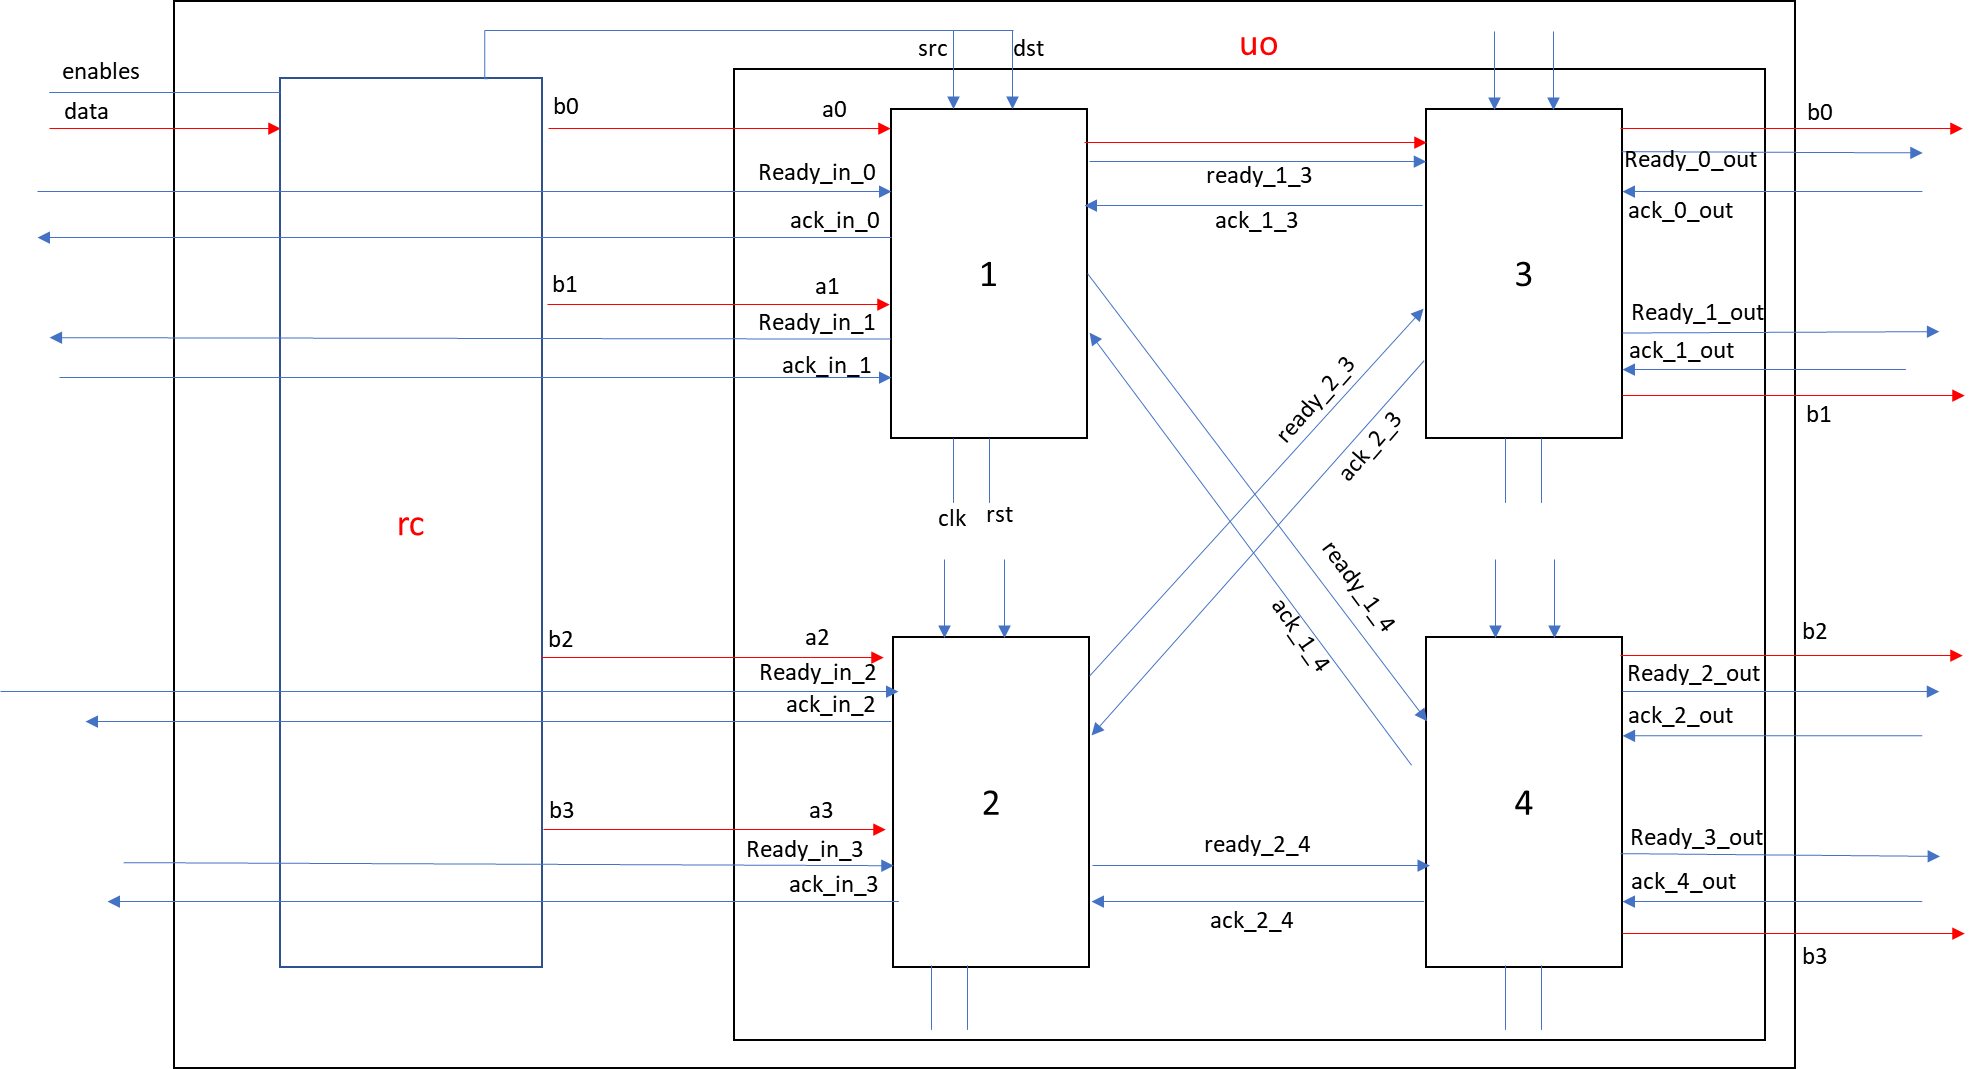
\includegraphics[width=15cm]{immagini/esercizio10/arch_tot_10.3.png}
    \caption{Architettura totale 10.3}
    \label{fig:sim_rc}
\end{figure}

\begin{lstlisting} [language=VHDL, caption=Rete di controllo switch]
library IEEE;
use IEEE.STD_LOGIC_1164.ALL;
use ieee.numeric_std.all;

entity rc_switch is
    port(
        clk, reset, ack0_snd, ready0_rcv, ack1_snd, ready1_rcv, dst, src: in std_logic;
        ack0_rcv, ready0_snd, ack1_rcv, ready1_snd,write_reg0, write_reg1: out std_logic
    );
end rc_switch;

architecture behavioral of rc_switch is
    type stato is (Q0, Q1, Q2, Q3, Q4, Q5, Q6);
    signal stato_corrente : stato:= Q0;
    signal stato_prossimo : stato;

begin
    comb: process(stato_corrente, ack0_snd, ready0_rcv, ack1_snd, ready1_rcv)

    begin
        case stato_corrente is
            when Q0=>
                stato_prossimo<=Q1;
                ready0_snd <= '0';
                ack0_rcv <= '0';
                ready1_snd <= '0';
                ack1_rcv <= '0';
                write_reg0<= '0';
                write_reg1<= '0';

            when Q1=>
                if (src = '0') then
                    if(ready0_rcv='1') then
                        stato_prossimo<=Q2;
                    else
                        stato_prossimo<=Q1;
                    end if;
                elsif (src ='1')  then
                    if(ready1_rcv='1') then
                        stato_prossimo<=Q2;
                    else
                        stato_prossimo<=Q1;
                    end if;
                end if;

            when Q2=>
                write_reg0<='1';
                write_reg1<= '1';
                stato_prossimo<=Q3;

            when Q3=>
                write_reg0<= '0';
                write_reg1<= '0';
                
                if (dst = '0') then
                    ready0_snd <= '1';
                elsif (dst ='1')  then
                    ready1_snd <= '1';
                end if;
                
                stato_prossimo<=Q4;

            when Q4=>
                 if (dst = '0') then
                    if(ack0_snd='1') then
                        stato_prossimo<=Q5;
                    else
                        stato_prossimo<=Q4;
                    end if;
                elsif (dst ='1')  then
                    if(ack1_snd='1') then
                        stato_prossimo<=Q5;
                    else
                        stato_prossimo<=Q4;
                    end if;
                end if;

            when Q5=>
                if (dst='0') then
                    ready0_snd <= '0';
                    elsif (dst='1') then
                        ready1_snd <= '0';
                end if;
                
                if (src='0') then
                    ack0_rcv <= '1';
                elsif (src='1') then
                    ack1_rcv <= '1';
                end if;
 
                stato_prossimo <=Q6;

            when Q6=>
                ack0_rcv<='0';
                ack1_rcv <= '0';
                stato_prossimo <=Q1;
            when others => stato_prossimo<= Q0;
        end case;
    end process comb;

    seq: process(clk)
    begin
        if rising_edge(clk) then
            if(reset='1')then
                stato_corrente<=Q0;
            else
                stato_corrente<=stato_prossimo;
            end if;
        end if;
    end process seq;
end behavioral;
\end{lstlisting}


Al contrario dell'esercizio precedente, questo \textit{switch} è una macchina sequenziale la cui implementazione è riportata nel listato di seguito.
\begin{lstlisting} [language=VHDL, caption=Switch sincrono]
library IEEE;
use IEEE.STD_LOGIC_1164.ALL;

entity switch is
    Port (
        src, dst, rst, clk, ack0_snd,ack1_snd, ready0_rcv,ready1_rcv: in std_logic;
        a0, a1: in std_logic_vector(1 downto 0);
        b0, b1: out std_logic_vector(1 downto 0);
        ack0_rcv, ack1_rcv, ready0_snd,ready1_snd: out std_logic
    );
end switch;

architecture Structural of switch is
    component mux_21 is
        Port (
            a0, a1: in std_logic_vector(1 downto 0);
            s : in std_logic;
            u : out std_logic_vector(1 downto 0)
        );
    end component mux_21;

    component demux_1_2 is
        port (
            a: in std_logic_vector(1 downto 0);
            s: in std_logic;
            u0, u1: out std_logic_vector(1 downto 0)
        );
    end component demux_1_2;

    component rc_switch is
        port(
            clk, reset, ack0_snd, ready0_rcv, ack1_snd, ready1_rcv, dst, src: in std_logic;
            ack0_rcv, ready0_snd, ack1_rcv, ready1_snd,write_reg0, write_reg1: out std_logic
        );
    end component rc_switch;

    component flip_flop is
        port (
            d: in std_logic_vector (1 downto 0);
            clk, reset: in std_logic ;
            write: in std_logic ;
            q:out std_logic_vector (1 downto 0));
    end component flip_flop;

    signal s_link, s_u0, s_u1: std_logic_vector(1 downto 0);
    signal s_write0, s_write1: std_logic;
begin

    m: mux_21 port map(
            a0=>a0,
            a1=>a1,
            s => src,
            u=>s_link
        );

    d: demux_1_2 port map(
            a=>s_link,
            u0=>s_u0,
            u1 => s_u1,
            s=>dst
        );

    ff1: flip_flop port map(
            d=>s_u0,
            q=>b0,
            clk=>clk,
            reset=>rst,
            write=>s_write0
        );

    ff2: flip_flop port map(
            d=>s_u1,
            q=>b1,
            clk=>clk,
            reset=>rst,
            write=>s_write1
        );

    rc: rc_switch port map(
            clk=>clk,
            reset=>rst,
            write_reg0=> s_write0,
            write_reg1=> s_write1,
            ack0_snd=>ack0_snd,
            ack1_snd=>ack1_snd,
            ready0_snd=> ready0_snd,
            ready1_snd=> ready1_snd,
            ack0_rcv=>ack0_rcv,
            ack1_rcv=>ack1_rcv,
            ready0_rcv=>ready0_rcv,
            ready1_rcv=>ready1_rcv,
            dst=>dst,
            src=>src
        );

end Structural;

\end{lstlisting}

\begin{lstlisting} [language=VHDL, caption=Arbitro]
library IEEE;
use IEEE.STD_LOGIC_1164.ALL;

entity unita_operativa is
  Port (
        a0, a1, a2, a3: in std_logic_vector(1 downto 0);
        src, dst: in std_logic_vector(1 downto 0);
        b0, b1, b2, b3: out std_logic_vector(1 downto 0);
        rst,clk: in std_logic ;
        
        ready_in_0,ready_in_1,ready_in_2,ready_in_3: in std_logic ;
        ack_in_0,ack_in_1,ack_in_2,ack_in_3: out std_logic ;
        ready_0_out, ready_1_out,ready_2_out,ready_3_out: out std_logic ;
        ack_0_out,ack_1_out,ack_2_out, ack_3_out: in std_logic
      
   );
end unita_operativa;

architecture Structural of unita_operativa is

component switch is
    Port (
        src, dst, rst, clk, ack0_snd,ack1_snd, ready0_rcv,ready1_rcv: in std_logic;
        a0, a1: in std_logic_vector(1 downto 0);
        b0, b1: out std_logic_vector(1 downto 0);
        ack0_rcv, ack1_rcv, ready0_snd,ready1_snd: out std_logic
    );
end component switch;
--dati
signal s_sw1_3, s_sw1_4,  s_sw2_3, s_sw2_4 : std_logic_vector(1 downto 0);

--ack e ready
signal s_ack_1_3, s_ack_1_4,s_ack_2_3,s_ack_2_4, s_ready_1_3, s_ready_1_4,s_ready_2_3,s_ready_2_4: std_logic;

begin

sw1: switch port map(
    src=>src(0),
    dst=>dst(1),
    a0=> a0,
    a1=> a1,
    
    ack0_rcv=> ack_in_0,
    ack1_rcv=> ack_in_1,
    
    ready0_snd=> s_ready_1_3,
    ready1_snd=> s_ready_1_4,
    
    ack0_snd=>s_ack_1_3,
    ack1_snd=>s_ack_1_4,
  
    ready0_rcv=> ready_in_0,
    ready1_rcv=> ready_in_1,    
    
    b0=> s_sw1_3,
    b1=> s_sw1_4,
    
    rst=> rst,
    clk=>clk
);

sw2: switch port map(
    src=>src(0),
    dst=>dst(1),
    a0=> a2,
    a1=> a3,
    
    ack0_rcv=> ack_in_2,
    ack1_rcv=> ack_in_3,
    
    ready0_snd=> s_ready_2_3,
    ready1_snd=> s_ready_2_4,
    
    ack0_snd=>s_ack_2_3,
    ack1_snd=>s_ack_2_4,
  
    ready0_rcv=> ready_in_2,
    ready1_rcv=> ready_in_3,    
    
    b0=> s_sw2_3,
    b1=> s_sw2_4,
    
    rst=> rst,
    clk=>clk
);


sw3: switch port map(
    src=>src(1),
    dst=>dst(0),
    a0=> s_sw1_3,
    a1=> s_sw2_3,
    
    ack0_rcv=> s_ack_1_3 ,
    ack1_rcv=> s_ack_2_3,
    
    ready0_snd=> ready_0_out,
    ready1_snd=> ready_1_out,
    
    ack0_snd=>ack_0_out,
    ack1_snd=>ack_1_out,
  
    ready0_rcv=> s_ready_1_3,
    ready1_rcv=> s_ready_2_3,    
    
    b0=> b0,
    b1=> b1,
    
    rst=> rst,
    clk=>clk
);

sw4: switch port map(
    src=>src(1),
    dst=>dst(0),
    a0=> s_sw1_4,
    a1=> s_sw2_4,
    
    ack0_rcv=> s_ack_1_4 ,
    ack1_rcv=> s_ack_2_4,
    
    ready0_snd=> ready_2_out,
    ready1_snd=> ready_3_out,
    
    ack0_snd=>ack_2_out,
    ack1_snd=>ack_3_out,
  
    ready0_rcv=> s_ready_1_4,
    ready1_rcv=> s_ready_2_4,    
    
    b0=> b2,
    b1=> b3,
    
    rst=> rst,
    clk=>clk
);

end Structural;
\end{lstlisting}

Infine, di seguito è presentato il codice dell'omega network \textbf{sincrona}:
\begin{lstlisting} [language=VHDL, caption=Omega Network]
library IEEE;
use IEEE.STD_LOGIC_1164.ALL;

entity omega_network is
    Port (
        a0,a1,a2,a3: in std_logic_vector (5 downto 0);
        en0, en1, en2, en3, clk, rst: in std_logic;
        b0,b1,b2,b3: out std_logic_vector (1 downto 0);

        ready_in_0,ready_in_1,ready_in_2,ready_in_3: in std_logic ;
        ack_in_0,ack_in_1,ack_in_2,ack_in_3: out std_logic ;
        ready_0_out, ready_1_out,ready_2_out,ready_3_out: out std_logic ;
        ack_0_out,ack_1_out,ack_2_out, ack_3_out: in std_logic

    );
end omega_network;

architecture Structural of omega_network is

    component unita_operativa is
        Port (
            a0, a1, a2, a3: in std_logic_vector(1 downto 0);
            src, dst: in std_logic_vector(1 downto 0);
            b0, b1, b2, b3: out std_logic_vector(1 downto 0);
            rst,clk: in std_logic ;

            ready_in_0,ready_in_1,ready_in_2,ready_in_3: in std_logic ;
            ack_in_0,ack_in_1,ack_in_2,ack_in_3: out std_logic ;
            ready_0_out, ready_1_out,ready_2_out,ready_3_out: out std_logic ;
            ack_0_out,ack_1_out,ack_2_out, ack_3_out: in std_logic

        );
    end component unita_operativa;

    component rete_di_controllo is
        port (
            a0, a1, a2, a3: in std_logic_vector(5 downto 0);
            en0, en1, en2, en3: in std_logic;
            b0, b1, b2, b3: out std_logic_vector(1 downto 0);
            src, dst: out std_logic_vector(1 downto 0)
        );
    end  component rete_di_controllo;

    signal  s_c0, s_c1, s_c2,  s_c3:  std_logic_vector(1 downto 0);
    signal s_src, s_dst :  std_logic_vector(1 downto 0);

begin

    rc: rete_di_controllo port map(
            a0 => a0,
            a1=> a1,
            a2=> a2,
            a3=> a3,
            en0=>en0,
            en1=>en1,
            en2=>en2,
            en3=>en3,
            b0=>s_c0,
            b1=> s_c1,
            b2=>s_c2,
            b3=>s_c3,
            src=>s_src,
            dst=>s_dst
        );

    uo: unita_operativa port map(
            a0 => s_c0,
            a1=> s_c1,
            a2=> s_c2,
            a3=> s_c3,
            src=>s_src,
            dst=>s_dst,
            b0=>b0,
            b1=> b1,
            b2=>b2,
            b3=>b3,
            clk=> clk,
            rst=> rst,

            ready_in_0=> ready_in_0,
            ready_in_1=>ready_in_1,
            ready_in_2=>ready_in_2,
            ready_in_3=>ready_in_3,
            ack_in_0=>ack_in_0,
            ack_in_1=>ack_in_1,
            ack_in_2=>ack_in_2,
            ack_in_3=>ack_in_3,
            ready_0_out=>ready_0_out,
            ready_1_out=>ready_1_out,
            ready_2_out=>ready_2_out,
            ready_3_out=>ready_3_out,
            ack_0_out=>ack_0_out,
            ack_1_out=>ack_1_out,
            ack_2_out=>ack_2_out,
            ack_3_out=>ack_3_out
        );

end Structural;

\end{lstlisting}

\subsection{Testing}
Per una maggiore sicurezza si è scelto di testare prima la rete di controllo dello \textit{switch} singolo, poi la rete di controllo dell'intero sistema (il cui test è omesso poiché analogo a quello dell'esercizio precedente) e infine si è effettuata la simulazione dell'omega network.

Di seguito è mostrato il \textit{testbench} della rete di controllo dello \textit{switch} il cui risultato è mostrato in 
 Figura \ref{fig:sim_rc_10_3}.
\begin{lstlisting} [language=VHDL, caption= Testing della rete di controllo dello switch]
library IEEE;
use IEEE.STD_LOGIC_1164.ALL;

entity switch_rc_TB is

end switch_rc_TB;

architecture Behavioral of switch_rc_TB is

component rc_switch is
    port(
        clk, reset, ack0_snd, ready0_rcv, ack1_snd, ready1_rcv, dst, src: in std_logic;
        ack0_rcv, ready0_snd, ack1_rcv, ready1_snd,write_reg0, write_reg1: out std_logic
    );
end component rc_switch;

    signal s_clk, s_reset, s_ack0_snd, s_ready0_rcv, s_ack1_snd, s_ready1_rcv, s_dst, s_src :  std_logic := '0';
    signal s_ack0_rcv, s_ready0_snd, s_ack1_rcv, s_ready1_snd, s_write_reg0, s_write_reg1 : std_logic := '0'; 

    constant clk_period:time:= 10ns;
begin

uut: rc_switch port map(
            clk=>s_clk,
            reset=>s_reset,
            write_reg0=> s_write_reg0,
            write_reg1=> s_write_reg1,
            ack0_snd=>s_ack0_snd,
            ack1_snd=>s_ack1_snd,
            ready0_snd=> s_ready0_snd,
            ready1_snd=> s_ready1_snd,
            ack0_rcv=>s_ack0_rcv,
            ack1_rcv=>s_ack1_rcv,
            ready0_rcv=>s_ready0_rcv,
            ready1_rcv=>s_ready1_rcv,
            dst=>s_dst,
            src=>s_src
        );

clock: process
    begin
           s_clk<= '1';
            wait for clk_period/2;
           s_clk <= '0';
            wait for clk_period/2;
    end process clock;

  tb: process
            begin
                wait for 100ns;
                s_reset<='1';
                wait for 10 ns;
                s_reset<='0';
                s_src<='0';
                s_dst <='0';
                wait for 10 ns;
                
                s_ready0_rcv <='1';
                wait for 30 ns;
                s_ready0_rcv <='0';
                wait for 30 ns;
                s_ack0_snd <='1';
                wait for 10 ns;
                s_ack0_snd <='0';
                wait for 40 ns;
                
                wait;
        end process tb;

end Behavioral;

\end{lstlisting}


\begin{figure}[H]
    \centering
    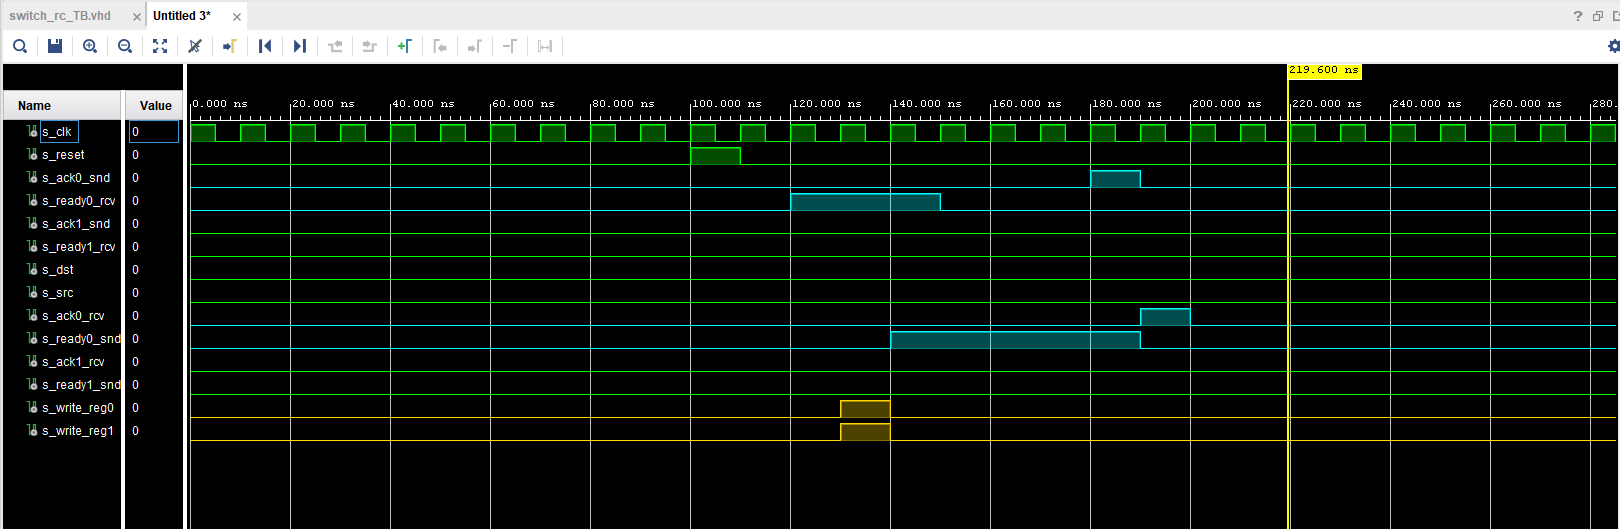
\includegraphics[width=15cm]{immagini/esercizio10/simulazione_rc_10.3.png}
    \caption{Testing rete di controllo switch}
    \label{fig:sim_rc_10_3}
\end{figure}


Infine, è presentato il \textit{testing} della \textit{omega network} sincrona con la simulazione in Figura \ref{fig:sim_on_sync}. 
\begin{lstlisting} [language=VHDL, caption=Testing dell'omega network]
library IEEE;
use IEEE.STD_LOGIC_1164.ALL;

entity omega_network_tb is
end omega_network_tb;

architecture Behavioral of omega_network_tb is

    component omega_network is
        Port (
            a0,a1,a2,a3: in std_logic_vector (5 downto 0);
            en0, en1, en2, en3, clk, rst: in std_logic;
            b0,b1,b2,b3: out std_logic_vector (1 downto 0);

            ready_in_0,ready_in_1,ready_in_2,ready_in_3: in std_logic ;
            ack_in_0,ack_in_1,ack_in_2,ack_in_3: out std_logic ;
            ready_0_out, ready_1_out,ready_2_out,ready_3_out: out std_logic ;
            ack_0_out,ack_1_out,ack_2_out, ack_3_out: in std_logic

        );
    end component omega_network;

    signal s_a0, s_a1, s_a2, s_a3 :  std_logic_vector(5 downto 0) := (others => '0');
    signal s_b0, s_b1, s_b2, s_b3 :  std_logic_vector(1 downto 0) := (others => '0');
    signal s_en0, s_en1, s_en2, s_en3, s_clk, s_rst :  std_logic := '0';
    signal s_ready_in_0,s_ready_in_1,s_ready_in_2,s_ready_in_3:  std_logic := '0';
    signal s_ack_in_0,s_ack_in_1,s_ack_in_2,s_ack_in_3:  std_logic := '0';
    signal s_ready_0_out, s_ready_1_out,s_ready_2_out,s_ready_3_out:  std_logic:= '0' ;
    signal s_ack_0_out,s_ack_1_out,s_ack_2_out, s_ack_3_out:  std_logic := '0';
    
    constant clk_period:time:= 10ns;

begin
    uut: omega_network port map(
            a0 => s_a0,
            a1=> s_a1,
            a2=> s_a2,
            a3=> s_a3,
            en0=>s_en0,
            en1=>s_en1,
            en2=>s_en2,
            en3=>s_en3,
            b0=>s_b0,
            b1=> s_b1,
            b2=>s_b2,
            b3=>s_b3,
            clk=> s_clk,
            rst=> s_rst,
            
            ready_in_0=> s_ready_in_0,
            ready_in_1=>s_ready_in_1,
            ready_in_2=>s_ready_in_2,
            ready_in_3=>s_ready_in_3,
            ack_in_0=>s_ack_in_0,
            ack_in_1=>s_ack_in_1,
            ack_in_2=>s_ack_in_2,
            ack_in_3=>s_ack_in_3,
            ready_0_out=>s_ready_0_out,
            ready_1_out=>s_ready_1_out,
            ready_2_out=>s_ready_2_out,
            ready_3_out=>s_ready_3_out,
            ack_0_out=>s_ack_0_out,
            ack_1_out=>s_ack_1_out,
            ack_2_out=>s_ack_2_out,
            ack_3_out=>s_ack_3_out
        );

    clock: process
    begin
        s_clk<= '1';
        wait for clk_period/2;
        s_clk <= '0';
        wait for clk_period/2;
    end process clock;

    process
    begin
        wait for 100ns;
        s_rst<='1';
        wait for 10 ns;
        s_rst<='0';
        wait for 10 ns;
        s_en0 <= '1';

        --dst --src  -a -r --data

        wait for 10 ns;
        s_a0 <= "010011";
        s_ready_in_0<='1';
        wait for 10 ns;
        s_ready_in_0<='0';
        wait for 10 ns;
        
        wait until s_ready_1_out='1';
        wait for 10 ns;
        s_ack_1_out<='1';
        wait for 10 ns;
        s_ack_1_out<='0';
        
        wait until s_ack_in_0='1';
        wait for 10 ns;
        
        report "received";
     wait;
    end process;

end Behavioral;

\end{lstlisting}


\begin{figure}[H]
    \centering
    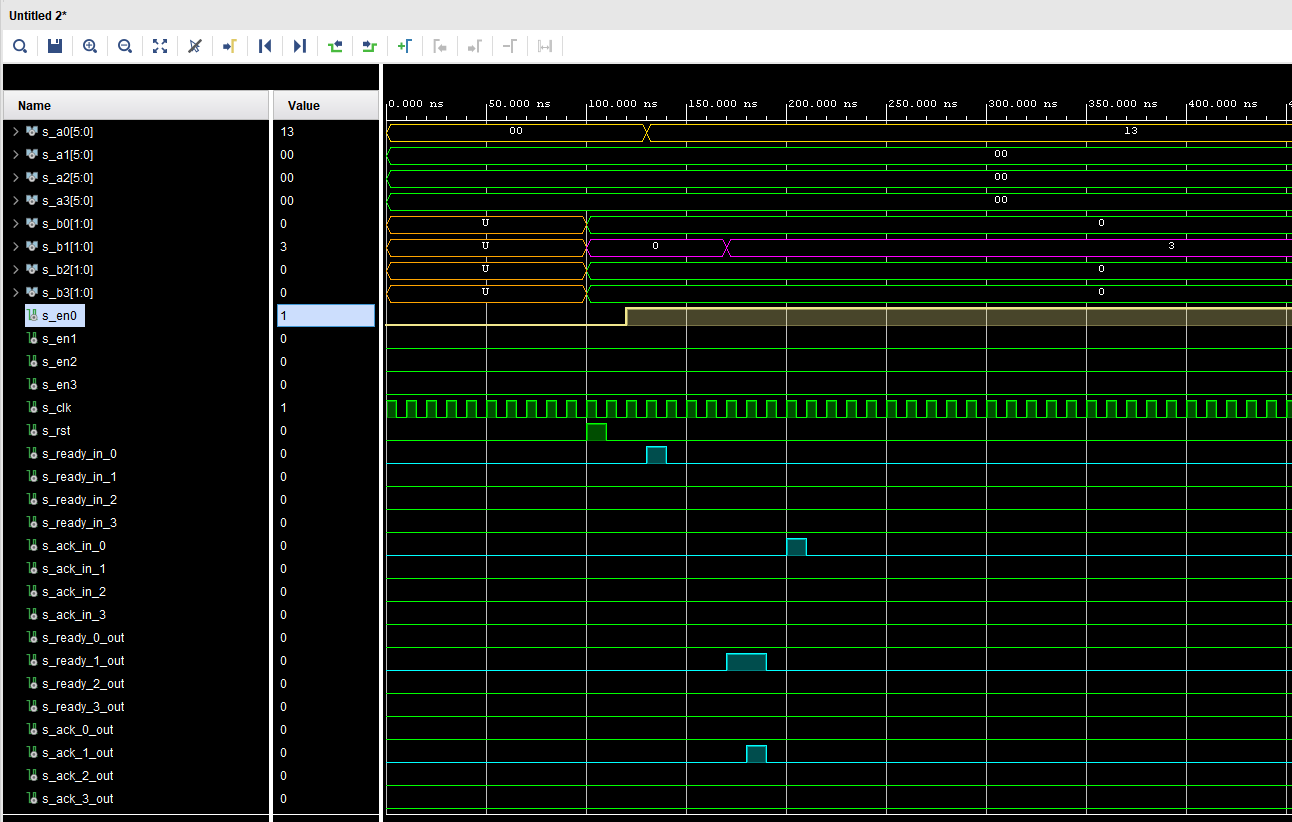
\includegraphics[width=15cm]{immagini/esercizio10/output_simulazione_10.3.png}
    \caption{Testing Omega Network sincrona}
    \label{fig:sim_on_sync}
\end{figure}

\chapter{Macchina aritmetica}

\section{Macchina aritmetica}

Progettare e implementare in VHDL una macchina aritmetica sequenziale a scelta fra le seguenti: 
    \begin{itemize}
        \item moltiplicatore di Robertson, per effettuare il prodotto di 2 stringhe A e B da 8 bit ciascuna;
        \item moltiplicatore di Booth, per effettuare il prodotto di 2 stringhe A e B da 8 bit ciascuna;
        \item divisore non-restoring, per effettuare la divisione intera fra due stringhe A e B di 4 bit ciascuna;
        \item divisore restoring, per effettuare la divisione intera fra due stringhe A e B di 4 bit ciascuna;
    \end{itemize}

Opzionalmente, la macchina implementata può essere sintetizzata su FPGA e testata mediante l’utilizzo dei dispositivi di input/output (switch, bottoni, led, display) presenti sulla board di sviluppo in dotazione al gruppo. La modalità di utilizzo degli stessi è a completa discrezione degli studenti.


\subsection{Il moltiplicatore di Robertson}
Si è scelto di implementare il moltiplicatore di Robertson. Nella prima sezione sarà descritta la parte architetturale con alcuni riferimenti teorici, mentre in quella successiva si scenderà nei dettagli implementativi e nel codice, esaminando il funzionamento della macchina attraverso i \textit{testbench}.

\subsubsection{Architettura}
L'architettura del sistema può essere suddivisa in due parti: l'unità di controllo e l'unità operativa.
Il sistema prende in ingresso i due operandi a 8 bit, i segnali di start, clock e reset e presenta in uscita il risultato della moltiplicazione a 16 bit, oltre che a due segnali di stop, che indicano la fine dell'operazione.
Dal seguente schema è possibile identificare i diversi componenti. Tutti i componenti diversi dalla UC (Unità di Controllo) costituiscono la parte operativa.
L'algoritmo manuale della moltiplicazione su N bit può essere formalizzato nella seguente espressione:
\begin{equation*}
  \mathlarger{\sum}_{i=0}^{N-1}X_i\cdot2^i\cdot Y
      \label{eq:mul_alg}
\end{equation*}


\begin{figure}[H]
    \centering
    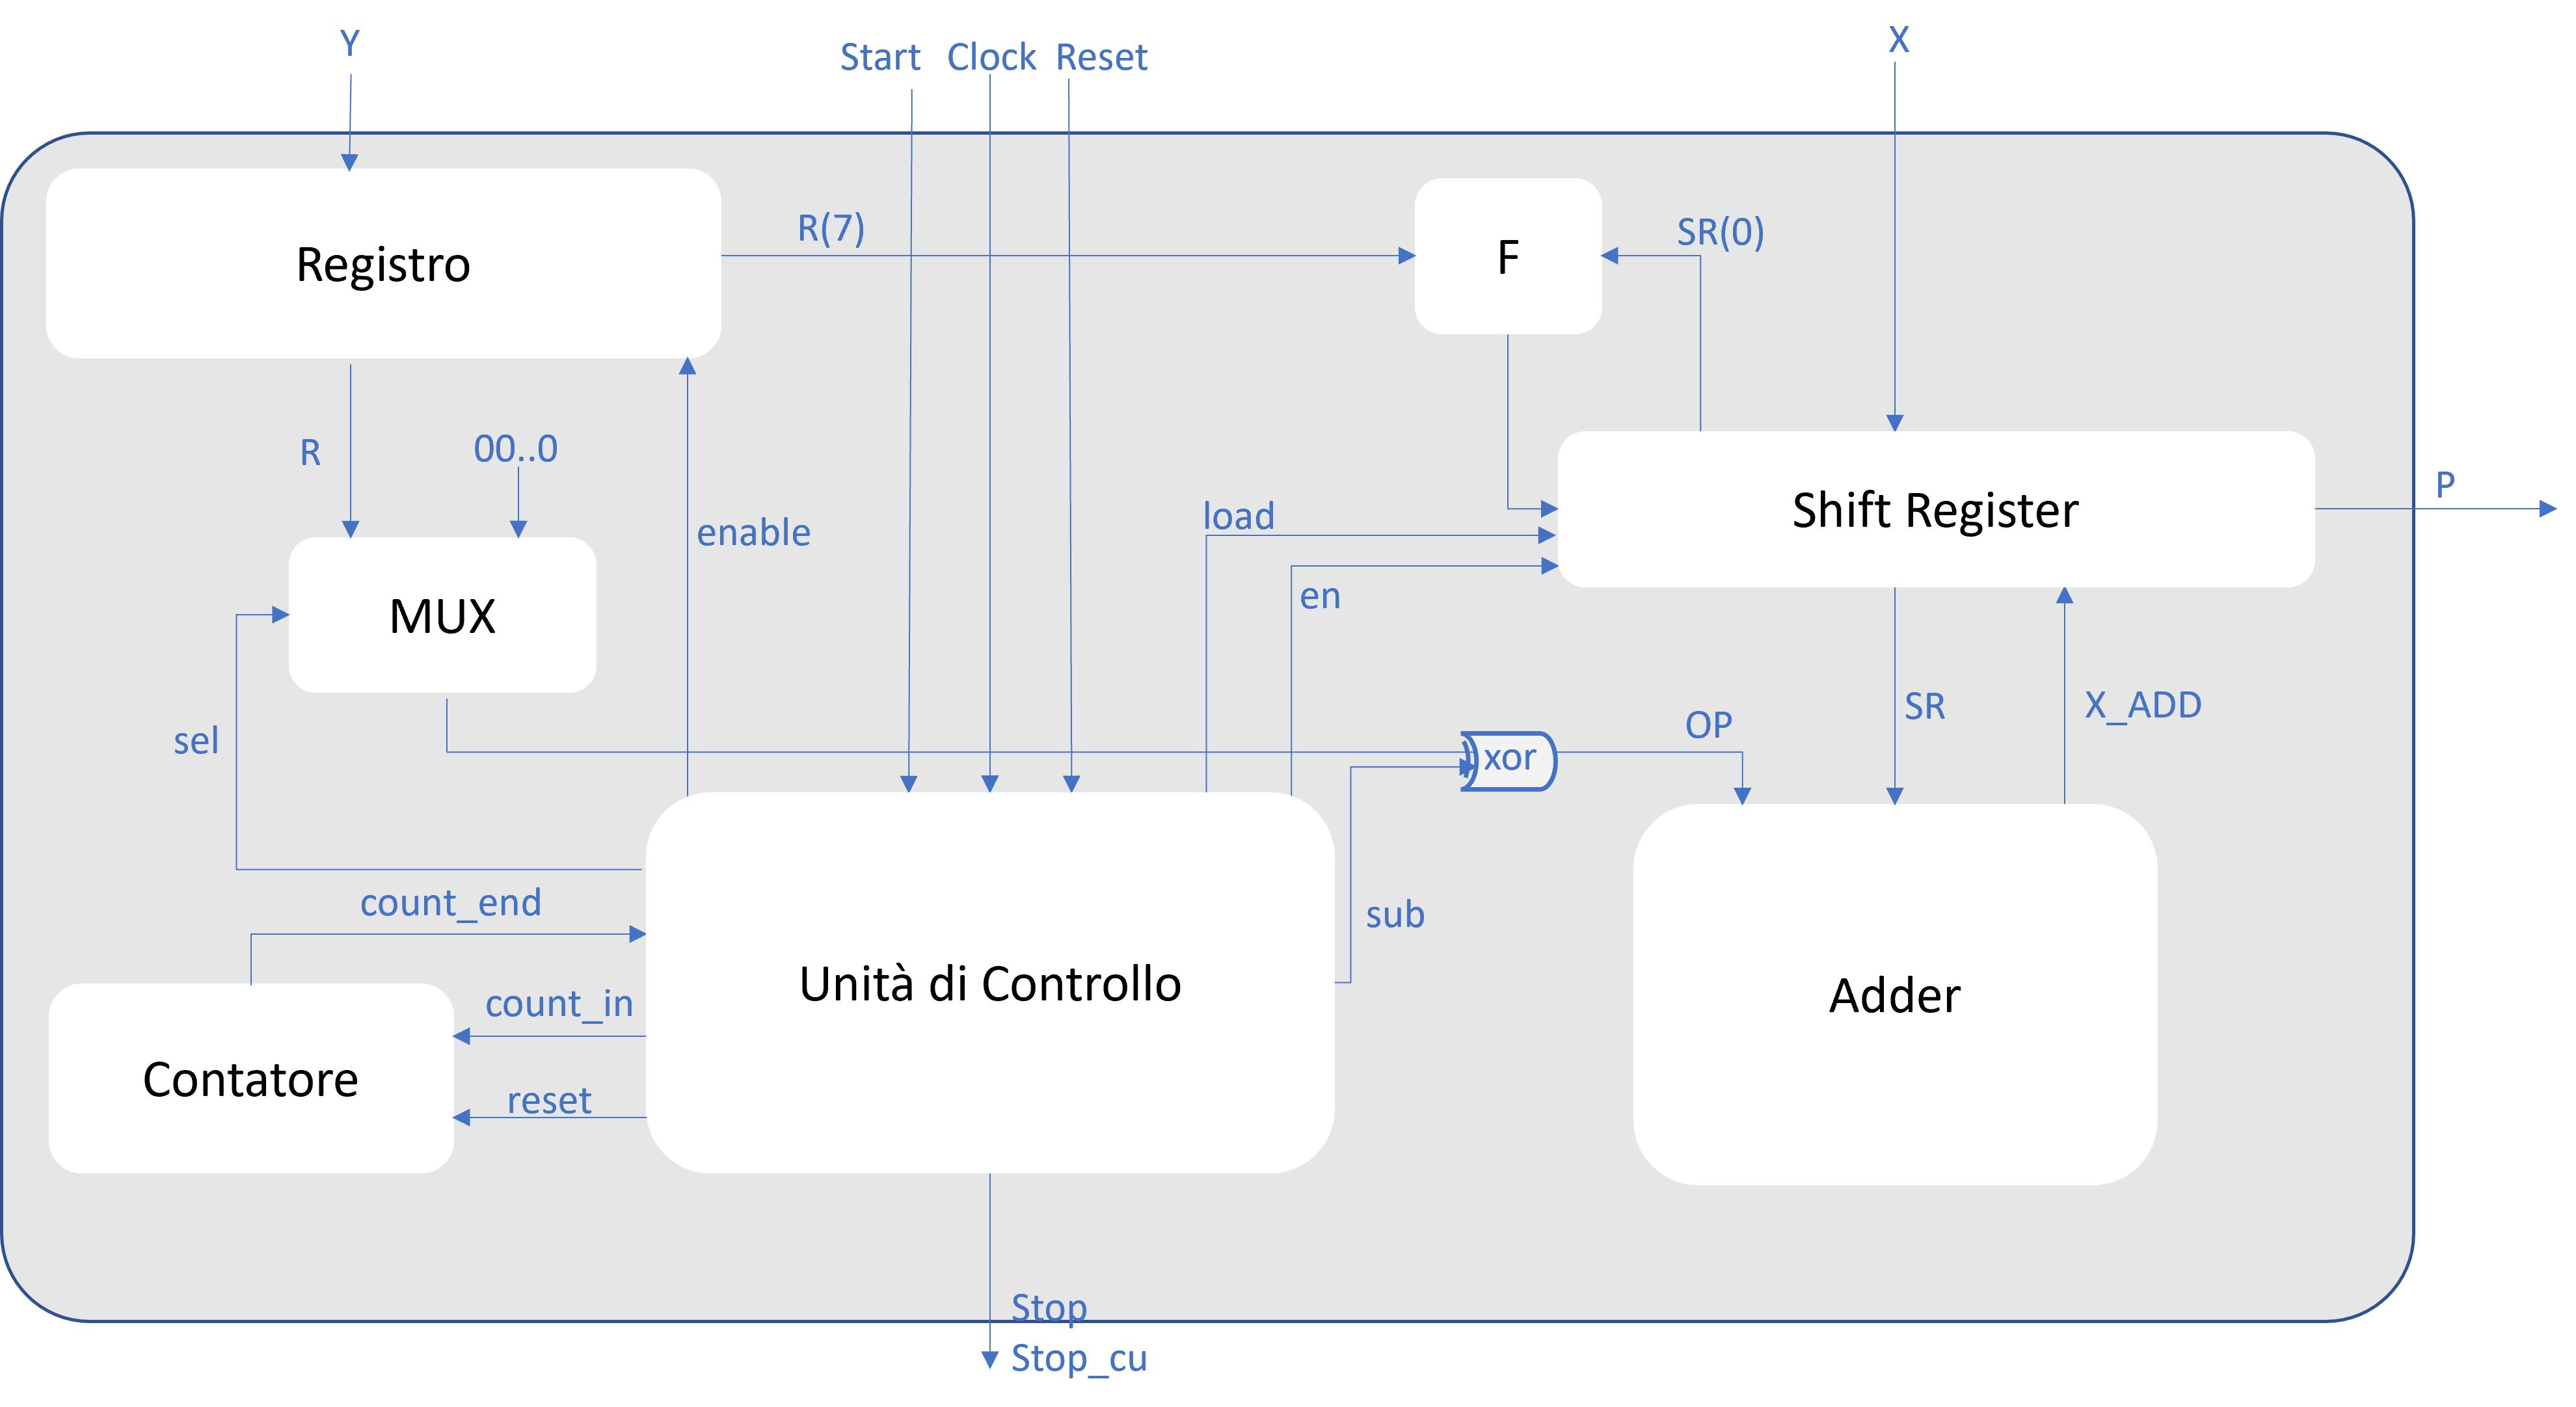
\includegraphics[width=17cm]{immagini/esercizio11/robertson_arch.png}
    \caption{Architettura moltiplicatore di Robertson}
    \label{fig:robertson_arch}
\end{figure}

L'unità operativa è formata dai seguenti componenti:
\begin{itemize}
\item \textbf{Shift register}: un registro a scorrimento a 16 bit in cui negli 8 meno significativi viene memorizzato l'operando X. L'unità di controllo decide se caricare l'operando o i risultati parziali del sommatore attraverso i segnali \textit{load} e \textit{load\_add}, e a ogni colpo di clock viene effettuato uno shift verso destra. Il motivo per cui si esegue lo \textit{shift} verso destra ha a che fare con l'algoritmo su cui si basa il moltiplicatore: partendo dall'algoritmo della moltiplicazione manuale, bisognerebbe variare il numero di \textit{shift} a sinistra in base al passo corrente durante (dalla Equazione \ref{eq:mul_alg} si vede che lo \textit{shift} dipende dalla $i$) il calcolo delle somme parziali. Per evitare questo problema si esegue prima la somma parziale e poi si scorre ogni volta verso destra di una sola posizione.

\item \textbf{Registro}:  un registro a 8 bit che memorizza il valore dell'operando Y. Oltre all'uscita a 8 bit che entra nel \textit{multiplexer}, contenente l'operando stesso, viene fornito il bit più significativo a F per il calcolo del segno.
\item \textbf{Contatore}: serve a contare i passi dell'unità di controllo. Quando arriva al massimo valore viene alzato il segnale \textit{cont\_end} e viene effettuata l'eventuale correzione che dipende dai segni degli operandi (come illustrato nella sezione dell'unità di controllo)
\item \textbf{Adder}: un \textit{ripple carry adder} che esegue le somme parziali e che è in grado anche di eseguire le sottrazioni. Per effettuare questo cambio, da somma a sottrazione, si usa un segnale di controllo sub che entra insieme all'uscita del \textit{multiplexer} (che conterrà Y) in una XOR, che a sua volta è collegata all'adder. In questo modo può essere calcolato -B in complementi a due. Per la somma normale l'entrata della XOR rappresenta invece il riporto entrante.
\item \textbf{F}: un registro che contiene il bit relativo al segno che viene calcolato come (Y(7) and X(0))or F).
\end{itemize}

L'unità di controllo è realizzata mediante un automa a stati finiti, il cui schema è mostrato in figura:

\begin{figure}[H]
    \centering
    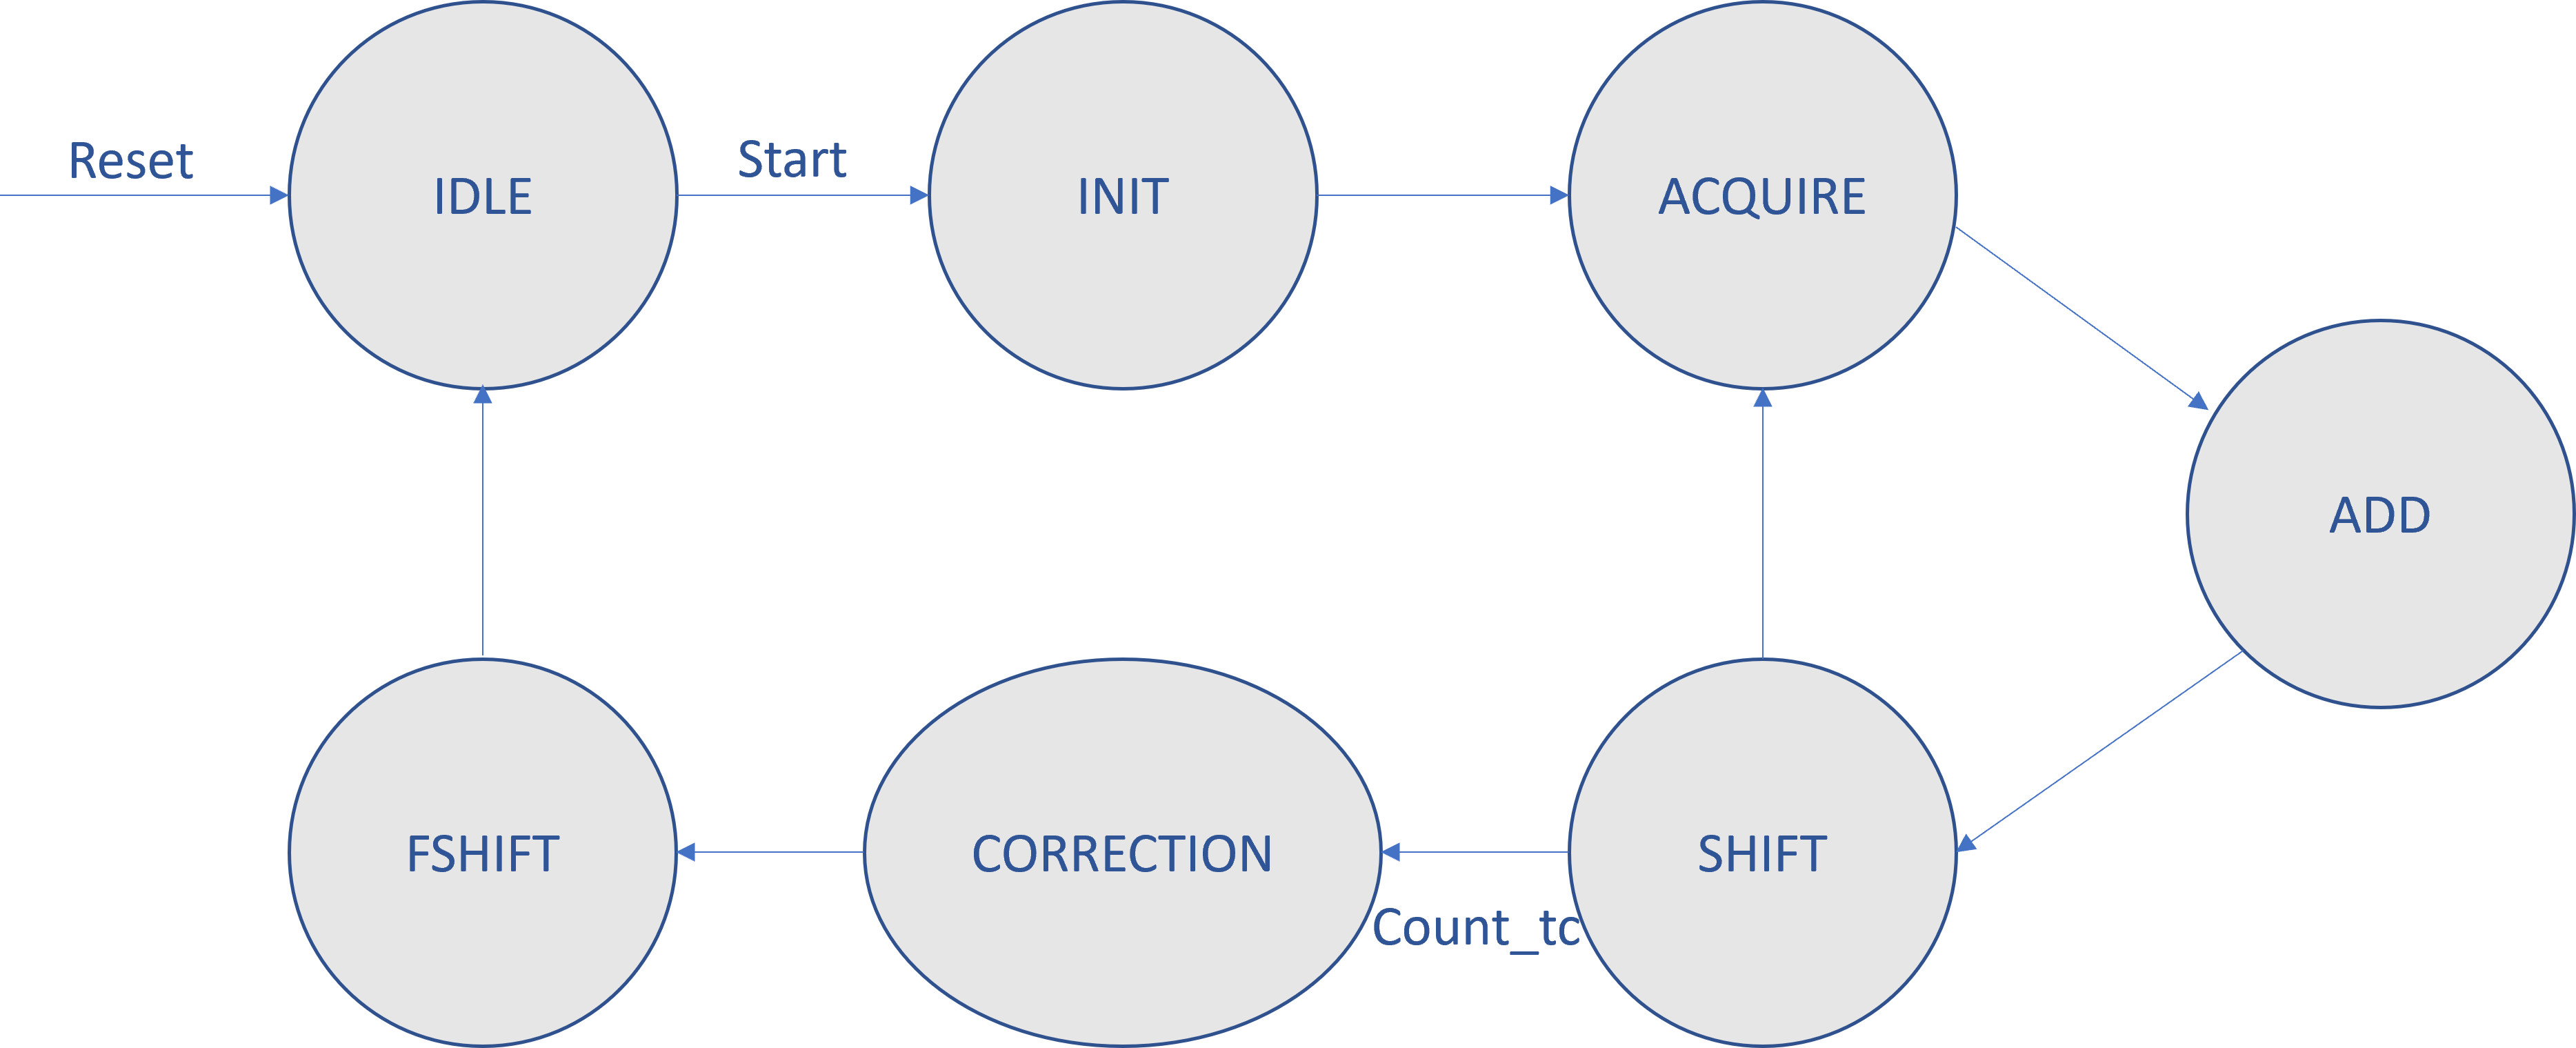
\includegraphics[width=14cm]{immagini/esercizio11/automa_robertson.png}
    \caption{Automa Moltiplicatore Robertson}
    \label{fig:robertson_automa}
\end{figure}

Di particolare importanza è il penultimo stato di correzione, necessario quando il risultato è negativo. Mentre il valore di Y è noto fin da subito, quindi non pone problemi anche nel caso sia negativo, X è conosciuto solo negli ultimi stati, dove a quel punto si è arrivati facendo la somma normale. Per far si che il risultato sia corretto vengono gestiti quindi i diversi casi:
\begin{itemize}
\item $X, Y >0$: non sono necessarie correzioni;
\item $X>0, Y<0$: grazie a F viene conservato il segno del prodotto negativo con Y, quindi non sono necessarie correzioni;
\item $X<0, Y>0$: è necessario il passo di correzione in cui si effettua la sottrazione al posto della somma;
\item $X, Y <0$: è necessario il passo di correzione per rendere il risultato positivo.
\end{itemize}


Nel listato \ref{robertson_op} è riportato il codice dell'unità operativa del molitplicatore di Robertson. Come descritto nell'architettura instanzia l'addizionatore (che può diventare un sottrattore a richiesta, invertendo il secondo operandoO), un registro a scorrimento (in cui sono memorizzati sia l'operando iniziale che il risultato finale) e un registro per il secondo operando e un contatore per tenere traccia dello stato delle operazioni.


\begin{lstlisting} [language=VHDL, label=robertson_op, caption=Unità operativa]
library IEEE;
use IEEE.STD_LOGIC_1164.ALL;
use IEEE.NUMERIC_STD.ALL;

entity unita_operativa is
	port( X, Y: in std_logic_vector(7 downto 0);
		  clock, reset, load, sub, sel: in std_logic;
		  en_SR, en_R8, en_D, count_in, load_add, shift, f_shift: in std_logic;
		  count: out std_logic_vector(2 downto 0);
		  P: out std_logic_vector(15 downto 0));
end unita_operativa;

architecture structural of unita_operativa is

	component adder_sub is
	port( X, Y: in std_logic_vector(7 downto 0);
		  cin: in std_logic;
		  Z: out std_logic_vector(7 downto 0);
		  cout: out std_logic);		  
	end component;
	
	component registro8 is 
	port( A: in std_logic_vector(7 downto 0);
		  clk, res,en: in std_logic;
		  B: out std_logic_vector(7 downto 0));
	end component;
	
	
	component mux_21 is
	port( x0, x1: in std_logic_vector(7 downto 0);
		  s: in std_logic;
		  y: out std_logic_vector(7 downto 0));
	end component;
	
	
	component shif_register is
	port( X: in std_logic_vector(15 downto 0);
		  F: in std_logic;
		  clock, reset, load, en, load_add, shift, f_shift:in std_logic;
		  x_add: in std_logic_vector(7 downto 0);
		  Y: out std_logic_vector(15 downto 0));	  
	end component;
	
	component FFD is
	port( clock, reset, d, en: in std_logic;
          y: out std_logic);
	end component;
	
	component cont_mod8 is
	port( clock, reset: in std_logic;
		  count_in: in std_logic;
		  count_end: out std_logic;
		  count: out std_logic_vector(2 downto 0));
	end component;


	signal temp1: std_logic_vector(7 downto 0);
	signal op1: std_logic_vector(7 downto 0);
	signal temp2: std_logic_vector(15 downto 0); 
	signal temp_p: std_logic_vector(15 downto 0);
	signal temp_d: std_logic :='0';
	signal temp_F: std_logic;
	signal tempadd: std_logic_vector(7 downto 0);
	signal riporto: std_logic;
	signal temp_countend: std_logic;
begin
	M: registro8 port map(Y, clock, reset, en_R8,temp1);
	MUX: mux_21 port map("00000000", temp1, sel, op1);
	
    temp2<="00000000" & X;
	SR: shif_register port map(temp2, temp_F, clock, reset, load, en_SR, load_add, shift, f_shift, tempadd, temp_p);
	temp_d<=(temp1(7) and temp_p(0)) or temp_F;
	D: FFD port map(clock, reset, temp_d, en_D, temp_F);
	ADD_SUB: adder_sub port map(temp_p(15 downto 8), op1, sub, tempadd, riporto);
	CONT: cont_mod8 port map(clock, reset, count_in, temp_countend, count);
	P<=temp_p;

end structural;
\end{lstlisting}

L'unità di controllo si occupa di implementare l'automa mostrato in Figura \ref{fig:robertson_automa}. Nel listato che segue è riportata l'implementazione.
\begin{lstlisting} [language=VHDL, label=robertson_rc, caption=Unità di Controllo]
library IEEE;
use IEEE.STD_LOGIC_1164.ALL;
use IEEE.NUMERIC_STD.ALL;

entity unita_controllo is 
	port( q0, clock, reset, start: in std_logic;
			count: in std_logic_vector(2 downto 0);
		  en_SR, en_R8, en_D, count_in, load_add, en_shift: out std_logic;
		  sel, reset_out, subtract, load, stop, en_fshift, stop_cu: out std_logic); 
end unita_controllo;

architecture Behavioral of unita_controllo is
	type state is (idle, init, acquisizione, add, shift, correzione, f_shift);
	signal current_state, next_state: state;

	begin 

	reg_stato: process(clock, reset)
			  begin
		      if(reset='1') then 
				current_state<=init;
			  elsif(clock'event and clock='1') then 
				current_state<=next_state;
			  end if;
			  end process;
			  
	comb: process(current_state, count)
		  begin
		  next_state<=idle;
		 
		  CASE current_state is
		  
		  WHEN idle => reset_out<='1';
					   en_D<='1';
					   en_R8<='1';
					   en_SR<='1';
					   count_in<='0'; 
					   subtract<='0';
					   load_add<='0';
					   load<='0';
					   sel<='0';
					   stop<='0';
						stop_cu<='0';
						en_fshift<='0';
						en_shift<='0';
					   if(start='1') then next_state<=init;
					   else next_state<=idle;
					   end if;
		--in ogni stato dobbiamo predisporre i valori dei segnali per lo stadio successivo
		  WHEN init => reset_out<='0'; 
		               count_in<='0';
					   load_add<='0';
					   en_D<='1';
					   en_R8<='1';
					   en_SR<='1';
					   load<='1';
					   subtract<='0';
					   stop<='0';
					   sel<=q0;
						en_shift<='0';
						en_fshift<='0';
						stop_cu<='0';
					   next_state<=acquisizione;
						
		--acquisisce gli operandi e predispone la add
		 WHEN acquisizione =>   en_SR<='1';
					  load<='0'; 
					  reset_out<='0'; 
					  en_D<='1';
					  load_add<='1';
					  en_R8<='1';
					  count_in<='1';
					  subtract<='0';
					  sel<=q0;
					  stop<='0';
					  stop_cu<='0';
					  en_fshift<='0';
					  en_shift<='0';
					  if(count="111") then 
									subtract<='1';
									next_state<=correzione;
									
					  else next_state<=add;
					  end if;
		--esegue la somma e predispone lo shift  
		 WHEN add =>  count_in<='0';
					  reset_out<='0'; 
		              sel<=q0;
					  subtract<='0';
					  load_add<='0'; 
					  en_SR<='1'; 
					  en_shift<='1';
					  load<='0'; 
					  en_D<='0';
					  en_R8<='1';
					  stop_cu<='0';
					  stop<='0';
					  en_fshift<='0';
					  next_state<=shift;
		--esegue lo shift e predispone per acquisizione	  
		WHEN shift => load<='0';
					  load_add<='0';
					  en_SR<='1'; --sr abilitato senza caricare x
					  reset_out<='0'; 
		           sel<=q0;
					  en_shift<='0';
					  count_in<='0';
					  subtract<='0';
					  en_D<='0';
					  en_R8<='1';
					  stop_cu<='0';
					  en_fshift<='0';
					  stop<='0';
					  next_state<=acquisizione;
	
	--in correzione fa la sottrazione e predispone per l'ultimo shift
		WHEN correzione => 	en_SR<='1';
							subtract<='0';
							load<='0'; 
							reset_out<='0'; 
							load_add<='0';
							en_D<='0'; --a(7)=a(7)
							en_R8<='1';
							count_in<='0';
							en_shift<='0';
							en_fshift<='1';
							sel<=q0;
							stop<='1';
							stop_cu<='0';
							next_state<=f_shift;
		
		WHEN f_shift => subtract<='0';
		                en_SR<='0';
						load<='0'; 
						reset_out<='0'; 
						load_add<='0';
						
						en_D<='0';
						en_R8<='1';
						en_shift<='0';
						en_fshift<='0';
						count_in<='0';
						sel<=q0;
						stop<='0';
						stop_cu<='1';
						next_state<=idle;
		  end CASE;
	end process; 
end Behavioral;

\end{lstlisting}


Infine sia unità operativa che controllo sono create e collegate in una unità che li racchiude, come mostrato nel listato \ref{robertson_top}.
\begin{lstlisting} [language=VHDL, label=robertson_top, caption= Robertson]
library IEEE;
use IEEE.STD_LOGIC_1164.ALL;
use IEEE.NUMERIC_STD.ALL;

entity Robertson is
	 port( clock, reset, start: in std_logic;
		   X, Y: in std_logic_vector(7 downto 0);		   
		   stop: out std_logic;		   
		   P: out std_logic_vector(15 downto 0);
		   stop_cu: out std_logic);
end Robertson;

architecture structural of Robertson is
	component unita_controllo is 
		port( q0, clock, reset, start: in std_logic;
			count: in std_logic_vector(2 downto 0);
		  en_SR, en_R8, en_D, count_in, load_add, en_shift: out std_logic;
		  sel, reset_out, subtract, load, stop, en_fshift, stop_cu: out std_logic);
	end component;
	
	component unita_operativa is
	port( X, Y: in std_logic_vector(7 downto 0);
		  clock, reset, load, sub, sel: in std_logic;
		  en_SR, en_R8, en_D, count_in, load_add, shift, f_shift: in std_logic;
		  count: out std_logic_vector(2 downto 0);
		  P: out std_logic_vector(15 downto 0));
	end component;
	
	signal tempq0, temp_sel, temp_clock, temp_res, temp_sub,temp_load: std_logic;
	signal temp_count: std_logic_vector(2 downto 0);
	signal temp_p: std_logic_vector(15 downto 0);
	signal ab_sr, ab_r8, ab_d, ab_c, t_load_add: std_logic;
	signal fine_conteggio: std_logic;
	signal temp_shift, temp_fshift: std_logic;
	
	begin
	
	UC: unita_controllo port map(tempq0, clock, reset, start, temp_count, ab_sr, ab_r8, ab_d, ab_c, t_load_add, temp_shift, temp_sel, temp_res, temp_sub, temp_load, stop, temp_fshift, stop_cu);
	UO: unita_operativa port map(X, Y, clock, temp_res, temp_load, temp_sub, temp_sel, ab_sr, ab_r8, ab_d,ab_c,t_load_add, temp_shift, temp_fshift, temp_count, temp_p); 
	tempq0<=temp_p(0);
	P<=temp_p;
	end structural;
\end{lstlisting}


\subsection{Simulazione}
Di seguito sono mostrate le simulazioni ottenute eseguendo il \textit{testbench} illustrato nel listato \ref{robertson_tb}. In particolare, sono presi in esame i seguenti casi:
\begin{itemize}
    \item Entrambi gli operandi sono positivi: la simulazione è mostrata in \ref{fig:robertson_sim_positivi}. Notiamo dagli stati attraversati dall'unità di controllo che non viene effettuata nessuna correzione;
     \item X negativo e Y positivo: la simulazione è mostrata in \ref{fig:robertson_sim_xneg_ypos}. In questo caso è necessaria una correzione poiché l'ultima cifra di X ha un peso negativo;
      \item X negativo e Y positivo: la simulazione è mostrata in \ref{fig:robertson_sim_xneg_yneg}. In questo caso è necessaria una correzione poiché il prodotto risulta negativo a causa del bit F. Bisogna effettuare una correzione facendo la sottrazione nelle somme parziali;
\end{itemize}

\begin{figure}[H]
    \centering
    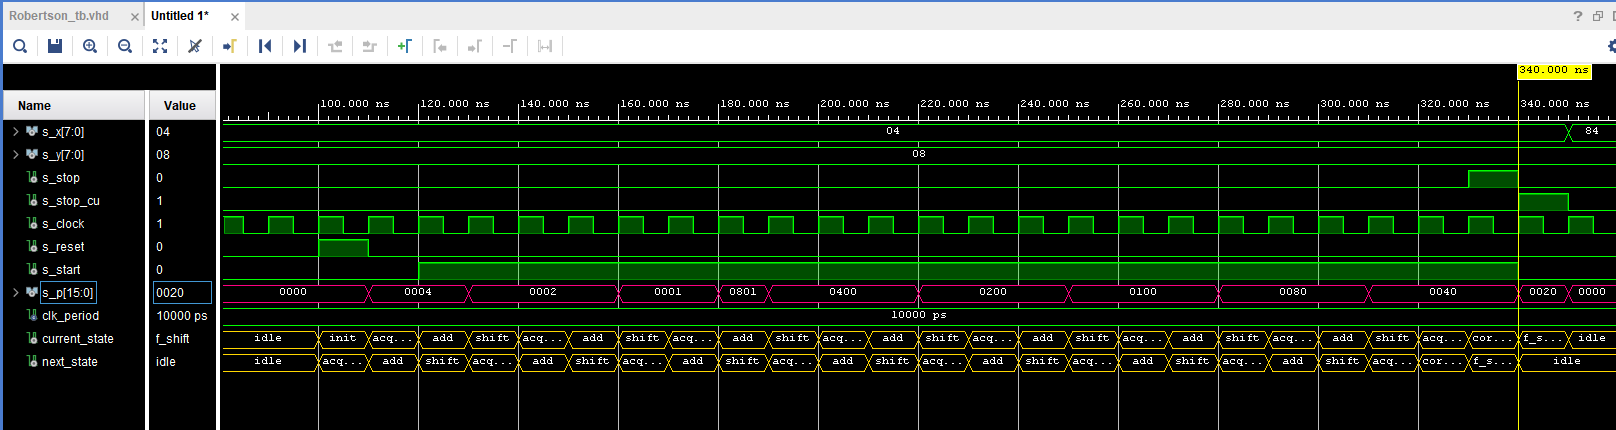
\includegraphics[width=16cm]{immagini/esercizio11/robertson_sim_xpos_ypos.png}
    \caption{Simulazione: X e Y positivi}
    \label{fig:robertson_sim_positivi}
\end{figure}

\begin{figure}[H]
    \centering
    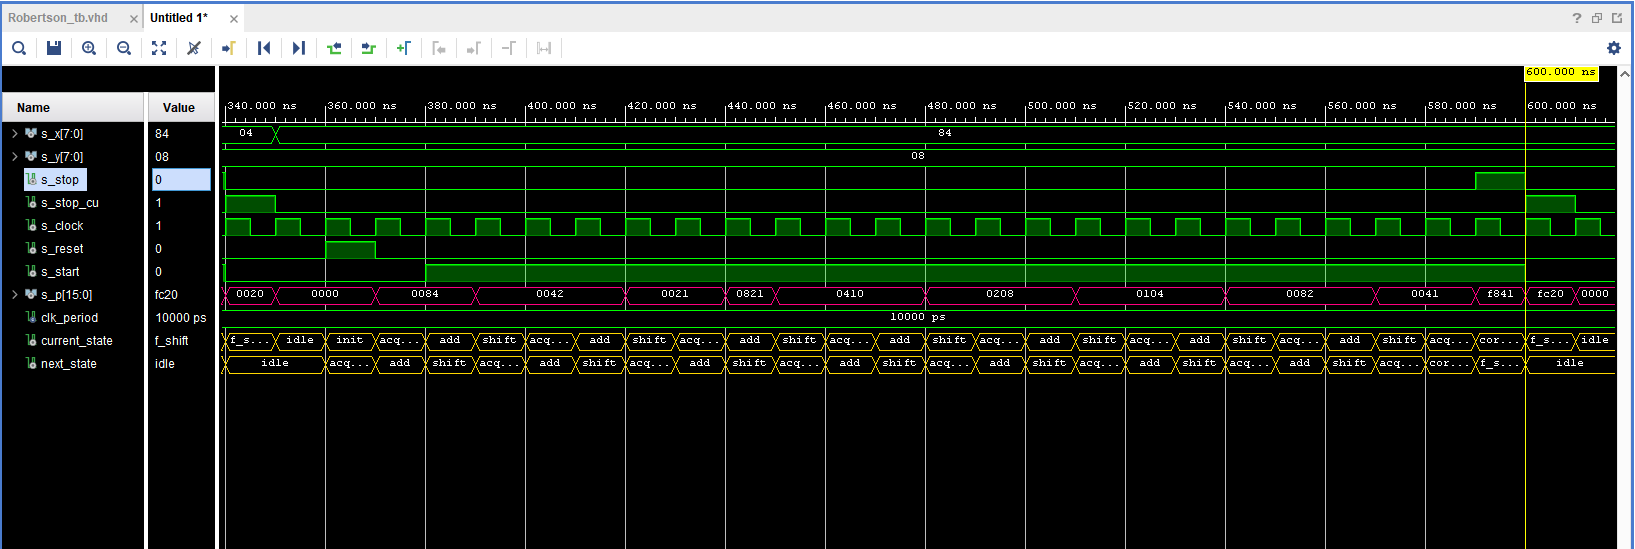
\includegraphics[width=16cm]{immagini/esercizio11/robertson_sim_xneg_ypos.png}
    \caption{Simulazione: X negativo e Y positivo}
    \label{fig:robertson_sim_xneg_ypos}
\end{figure}

\begin{figure}[H]
    \centering
    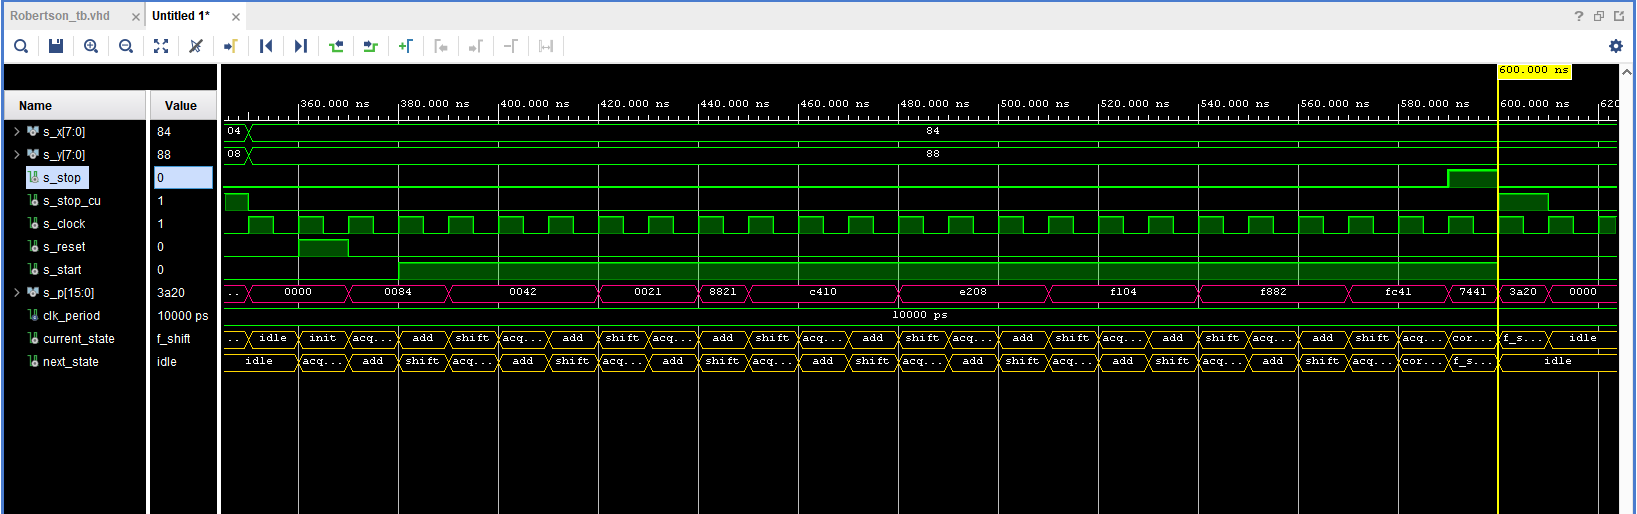
\includegraphics[width=16cm]{immagini/esercizio11/robertson_sim_xneg_yneg.png}
    \caption{Simulazione: X e Y negativi}
    \label{fig:robertson_sim_xneg_yneg}
\end{figure}


\begin{lstlisting} [language=VHDL, label=robertson_tb, caption=Testbench moltiplicatore di Robertson]
library IEEE;
use IEEE.STD_LOGIC_1164.ALL;
use IEEE.numeric_std;

entity Robertson_tb is
    --  Port ( );
end Robertson_tb;

architecture Behavioral of Robertson_tb is

    component  Robertson is
        port( clock, reset, start: in std_logic;
             X, Y: in std_logic_vector(7 downto 0);
             stop: out std_logic;
             P: out std_logic_vector(15 downto 0);
             stop_cu: out std_logic);
    end component Robertson;

    signal s_x, s_y: std_logic_vector (7 downto 0):="00000000";
    signal s_stop, s_stop_cu, s_clock, s_reset,s_start: std_logic:='0' ;
    signal s_p: std_logic_vector (15 downto 0):="0000000000000000";
    constant clk_period: time := 10ns;

begin

    uut: Robertson port map(
            clock=>s_clock ,
            reset=> s_reset ,
            start=> s_start,
            X=> s_x,
            Y=> s_y,
            stop=> s_stop,
            P=> s_p,
            stop_cu=> s_stop_cu
        );

    clock: process
    begin
        loop
            s_clock <= not s_clock;
            wait for clk_period/2;
        end loop;
    end process clock;

    process
    begin
    
    s_x<="00000100";
    s_y<="00001000";
    
    wait for 100ns;
    s_reset <= '1';
    wait for clk_period;
    s_reset <= '0';
    wait for clk_period;
    s_start <='1';

    wait until s_stop_cu='1';
    s_start <='0';
    
    wait for 10ns;

    s_x<="10000100";
    s_y<="00001000";
    
    wait for 10ns;
    s_reset <= '1';
    wait for clk_period ;
    s_reset <= '0';
    wait for clk_period ;
    s_start <='1';

    wait until s_stop_cu='1';
    s_start <='0';
  
   
    wait for 10ns;

    s_x<="10000100";
    s_y<="10001000";
    
    wait for 10ns;
    s_reset <= '1';
    wait for clk_period ;
    s_reset <= '0';
    wait for clk_period ;
    s_start <='1';

    wait until s_stop_cu='1';
    s_start <='0';
  
    wait;

    end process;

end Behavioral;

\end{lstlisting}

\chapter{Esercizio a scelta}
\section{Traccia}

 Modifica di esercizi già proposti (processore, rete di interconnessione o interfaccia seriale) mediante aggiunta/aggiornamento di funzionalità. 
Esempio: si potrebbe pensare di modificare l’interfaccia seriale aggiungendo segnali specifici per l’\textit{handshaking} fra due entità. 

\subsection{Descrizione esercizio}
Partendo da gli esercizi numero 7 e 9 si è scelto di creare un unico sistema che comprende le funzionalità di trasmissione seriale ripetuta, tracciata da un contatore, la sincronizzazione tramite three-way handshake e la lettura e scrittura su memoria con l'esecuzione di un'operazione di somma.


\subsection{Architettura}
L'architettura unisce diversi aspetti degli esercizi precedenti. Ci sono due componenti, A e B che comunicano tramite un'interfaccia seriale UART. Le due unità di controllo in A e B sono connesse con tre segnali per effettuare il three-way handshake necessario alla sincronizzazione della trasmissione.

Il sistema A è composto da:
\begin{itemize}
    \item \textit{ROM}: è una memoria che contiene le N stringe di 8 bit da dover mandare al sistema B;
    \item \textit{UART}: il componente, fornitoci a priori, costituisce in un'interfaccia per la trasmissione del dato tra i due sistemi;
    \item \textit{contatore}: conta il numero di trasmissioni effettuate;
    \item \textit{rete di controllo}: regola che la trasmissione dei dati avvenga in modo corretto.
\end{itemize}

Il sistema B, invece, è composto da:
\begin{itemize}
    \item \textit{registro}: un flip flop che memorizza la stringa ricevuta dal sistema A;
    \item \textit{UART}: il componente, fornitoci a priori, costituisce in un'interfaccia per la ricezione del dato ;
    \item \textit{contatore}: conta il numero di trasmissioni effettuate, nonché il numero di somme effettuate;
    \item \textit{ROM}: è una memoria che contiene le N stringe da sommare;
    \item \textit{rete di controllo}: regola che la trasmissione e l'output dei dati avvenga in modo corretto.
\end{itemize}

L'interconnessione tra i due sistemi è visibile nella seguente architettura: 
\begin{figure}[H]
    \centering
    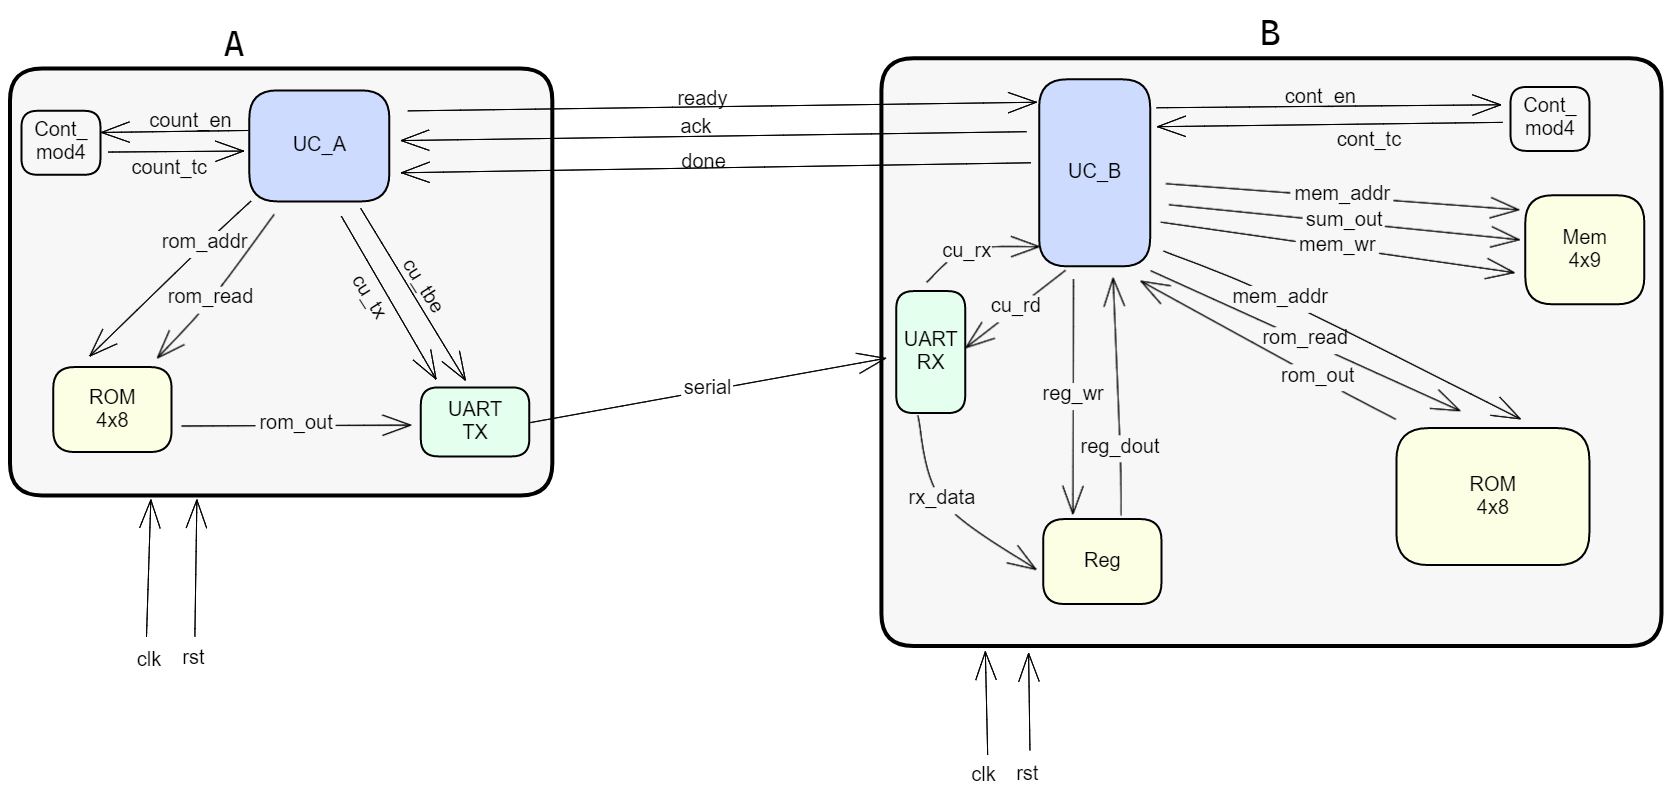
\includegraphics[width=16cm]{immagini/esercizio12/schema_12.png}
    \caption{Schema Interfaccia Seriale}
\end{figure}

Gli automi di A e B sono basati su quelli visti nei precedenti esercizi ma hanno subito diverse modifiche.
Nel sistema A prima di poter abilitare il segnale di \textit{ready} viene effettuata la lettura dalla memoria ROM in cui sono contenuti i dati da trasmettere. Successivamente si aspetta l'ack del sistema B, che indica la sua disponibilità a ricevere il dato. Questo punto è essenziale, poichè significa che B ha impostato il ricevitore UART in modo opportuno. Superato l'ack l'automa controlla che il segnale tbe sia uguale a 1. In caso contrario, significa che il trasmettitore è occupato, e non può ancora inviare messaggi. Appena il trasmettitore è pronto, viene alzato cu\_tx e si aspetta la fine della ricezione del dato da parte di B, indicata dal segnale \textit{done}.\\

È da notare che allo stato successivo è stato inserito un altro auto-anello che aspetta che il \textit{done} si abbassi. Questo stato serve per evitare che il cambiamento del segnale \textit{done} risvegli il processo durante uno stato sensibile, come ad esempio quello in cui si incrementa l'indirizzo (si avrebbe un incremento doppio). Non è possibile per A controllare quando il segnale \textit{done} varierà, e questa misura quindi si aggiunge alle regole del protocollo stabilito che mira ad incrementare l'affidabilità della trasmissione. \\

Si sarebbero potute implementare soluzioni alternative, come l'utilizzo di clock più lenti o l'aggiunta di stati, ma questa soluzione con il ciclo permette all'automa di funzionare a prescindere dalla tecnologia sottostante, senza andare a inficiare sui tempi del clock.

Infine, viene incrementato il contatore e l'indirizzo di memoria, e si esegue il controllo sul \textit{count\_tc}. Una volta alzato infatti, l'automa arriverà allo stato \textit{idle} e fermerà le trasmissioni.


L'automa di B aspetta e alza i segnali ready e ack in modo duale ad A , e una volta arrivato il messaggio, notificato dal segnale alto \textit{RDA (uc\_rx)} scrive il risultato in un registro temporaneo. A questo punto l'interfaccia UART è libera, e si procede alla lettura della ROM di B e alla somma con il dato appena arrivato. Finita la somma, a cui è stato dato il tempo di finire con uno stato a se, il risultato viene scritto in una memoria e si controlla se si è arrivati al massimo delle ricezioni possibili. 

Di seguito è possibile osservare la stesura degli automi dei singoli sistemi: 
\begin{figure}[H]
    \centering
    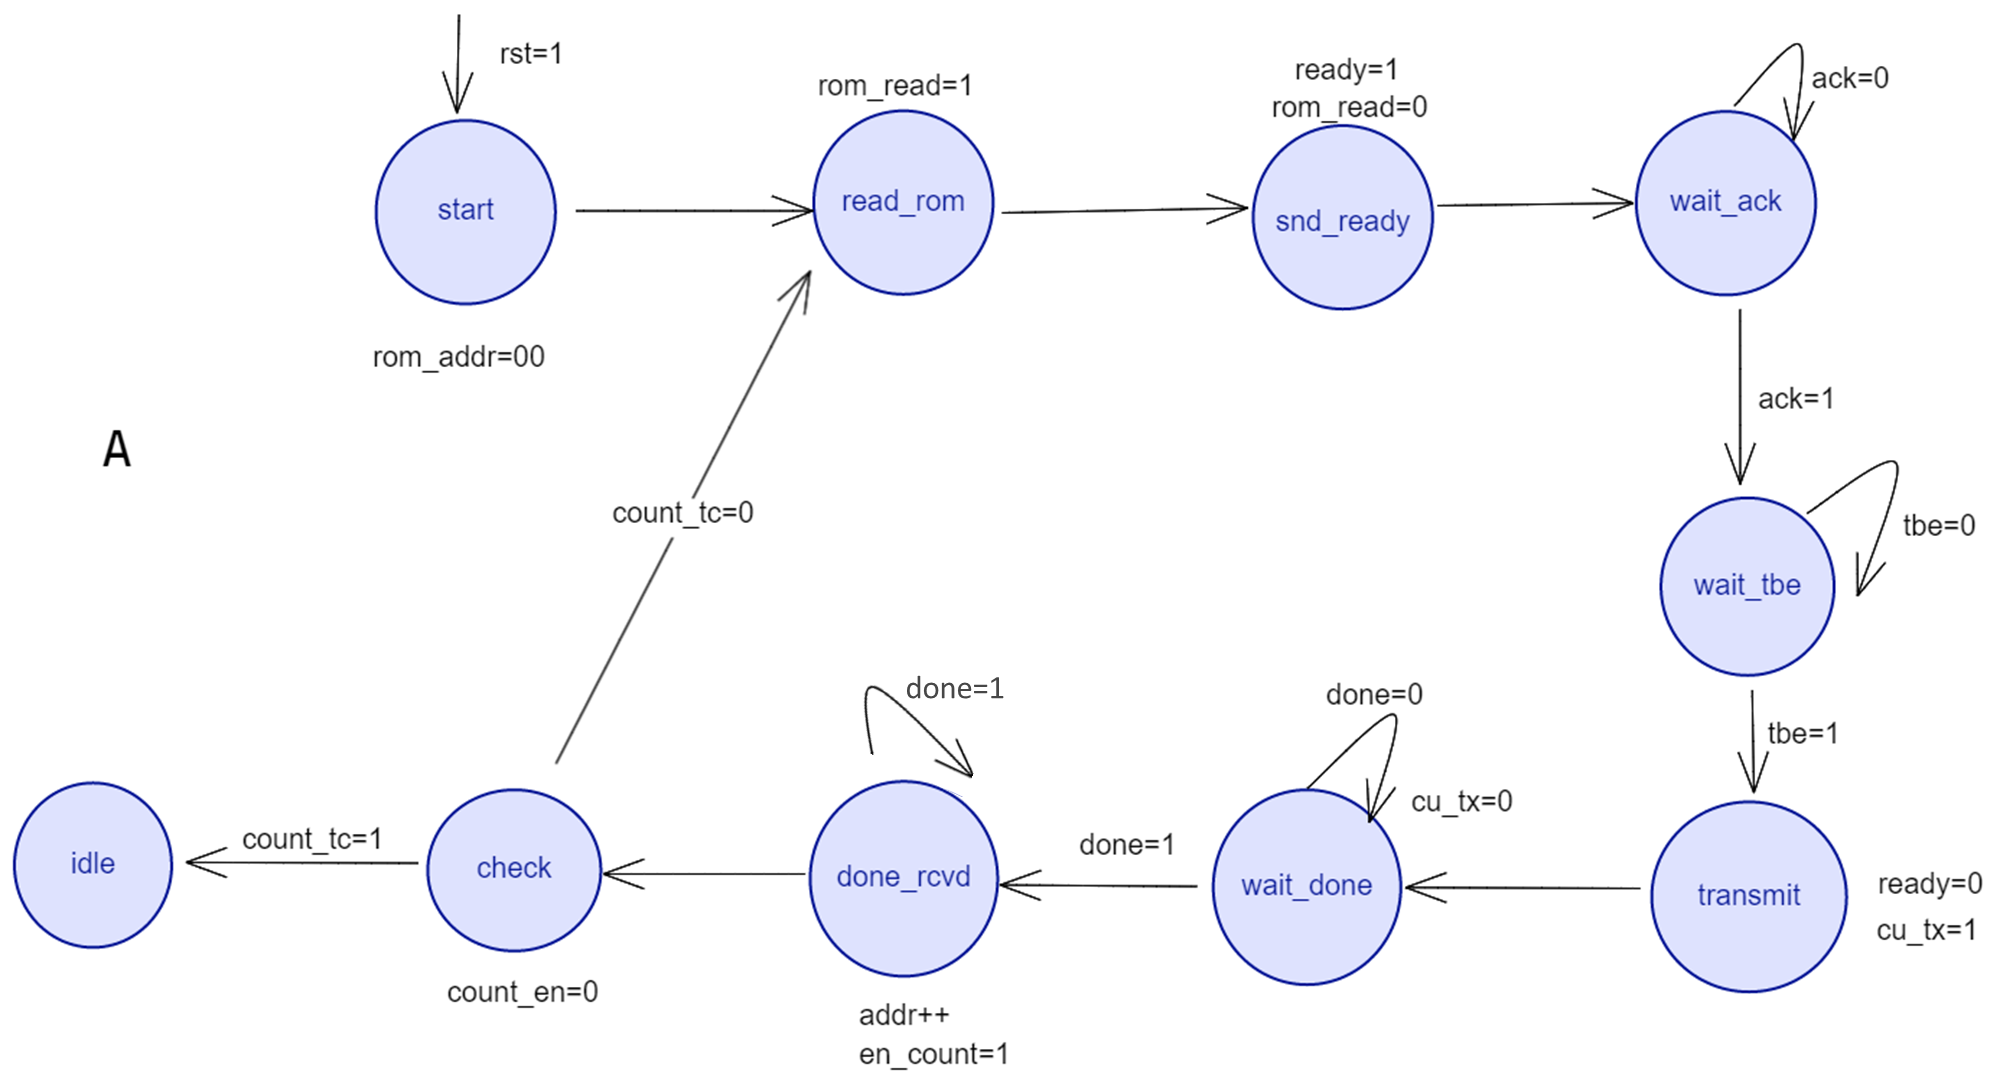
\includegraphics[width=16cm]{immagini/esercizio12/automaA_12.png}
    \caption{Automa A}
\end{figure}

\begin{figure}[H]
    \centering
    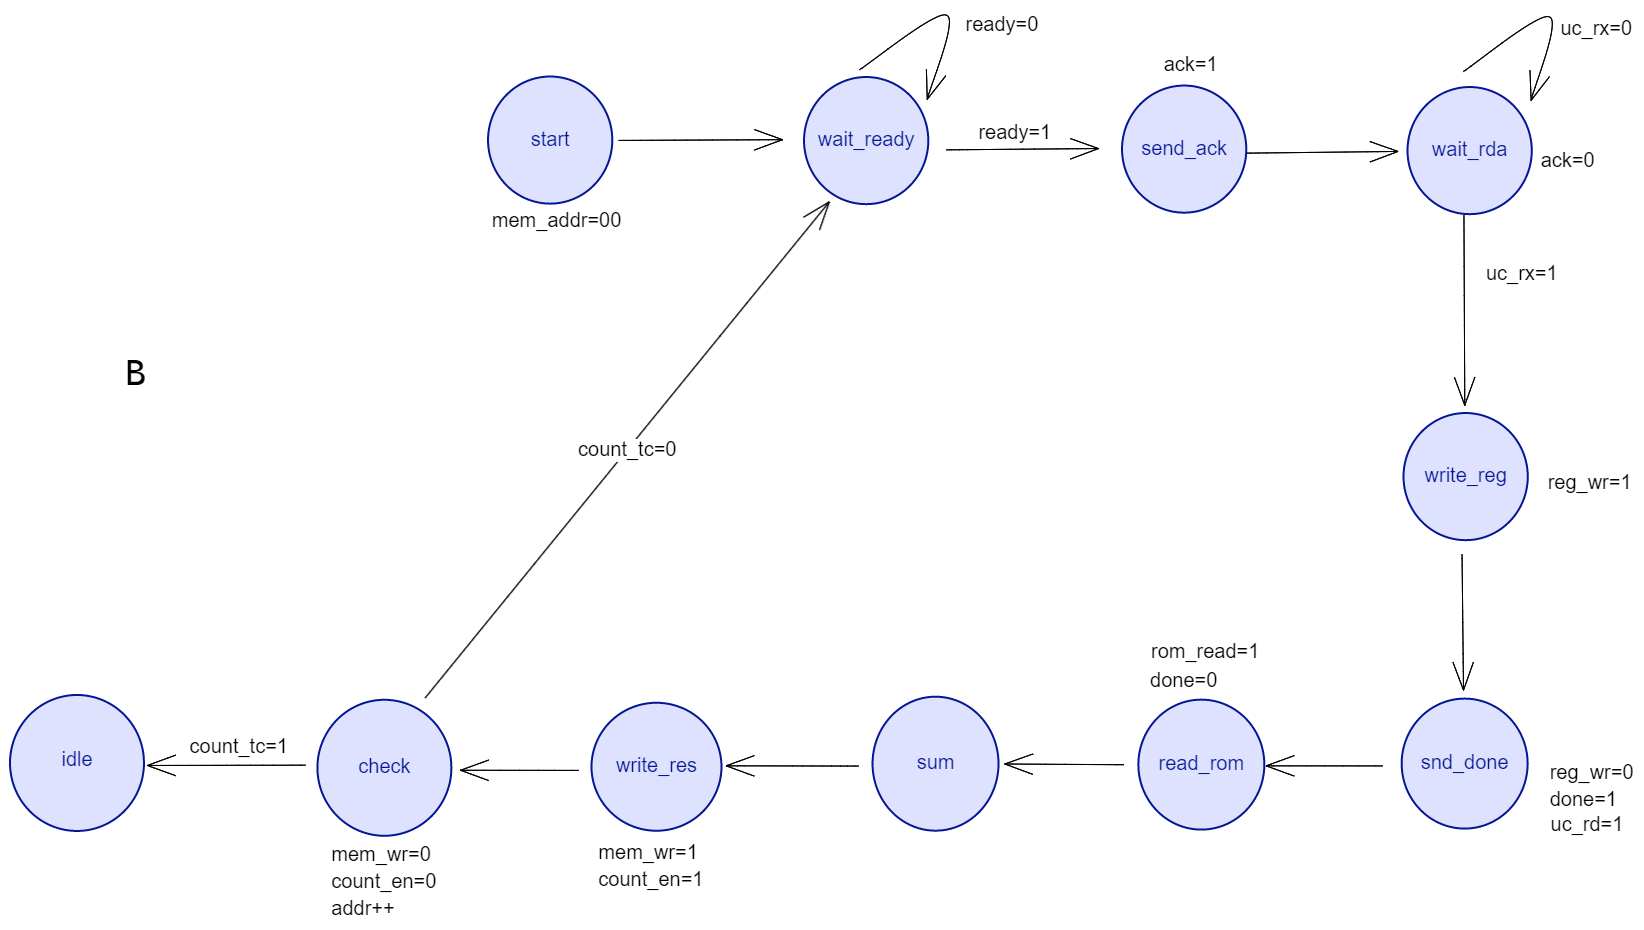
\includegraphics[width=16cm]{immagini/esercizio12/automaB_12.png}
    \caption{Automa B}
\end{figure}

\subsection{Analisi}
\subsubsection{UART vs USART}
L'idea della soluzione si basa sul confronto tra UART e USART e le performance nettamente superiori della versione sincrona rispetto a quella asincrona. In particolare, in Tabella \ref{tab:uart_usart}, sono analizzate le differenze tra le due tecnologie.

\begin{table}
    \centering
    \begin{tabular}{|p{5cm}||p{5cm}| }
        \hline
        UART & USART \\ [0.5ex] 
         \hline\hline
         \hline
            Può comunicare sia in \textit{half-duplex} che \textit{full-duplex} & Può comunicare \textbf{solo} in modalità \textit{half-duplex} \\
         \hline 
         \hline
           Invia dati con \textit{rate} diversi, di solito più basso rispetto all'USART & Invia dati con un rate fisso  \\
         \hline
            Sorgente e destinazione devono essere configurati con i parametri corretti del \textit{baud rate} & Sorgente e destinazione non hanno bisogno di conoscere nulla dei rispettivi \textit{clock} \\
         \hline
         Invia un byte per volta & Può inviare pacchetti più grandi \\
         \hline
          
    \end{tabular}
    \caption{Confronto tra UART e USART}
    \label{tab:uart_usart}
\end{table}


Uno dei motivi per cui è molto diffuso UART è per la sua facilità di implementazione. Con l'approccio scelto si preserva la semplicità, ma si aggiunge un grado di affidabilità alla comunicazione. Inoltre, utilizzando la periferica UART è possibile continuare ad effettuare comunicazioni \textit{full-duplex}.



\subsubsection{Three-way-handshake vs Two-way-handshake}

Nell'esercizio svolto, sono combinati i benefici sia del mondo sincrono che quello asincrono. Infatti, la soluzione prevede di implementare l'handshake e quindi la gestione della sincronizzazione tra le due entità al di fuori della periferica UART. In questo modo, la comunicazione risulta sincrona (anche se i due sistemi devono conoscere il \textit{baud rate}), e in caso di errori di trasmissione, il ricevitore può usare il segnale \textit{done} per codificare una politica di gestione del \textit{fault}. Ad esempio, immaginando di avere più bit per il segnale \textit{done}, può essere codificato un codice di risposta in cui si richiede una ritrasmissione.


Di seguito è riportato il codice dell'intera soluzione, omettendo i componenti elementari quali flip flop e memoria già descritti nei capitoli precedenti.
\begin{lstlisting} [language=VHDL, caption=Rete di controllo di A]
library IEEE;
use IEEE.STD_LOGIC_1164.ALL;
use IEEE.numeric_std.all;

entity cu_a is
    port(
        clk, rst, ack, done, count_tc, cu_tbe: in std_logic;
        ready, cu_tx, rom_read, count_en: out std_logic;
        rom_addr: out std_logic_vector(1 downto 0)
    );
end cu_a;

architecture behavioral of cu_a is

    type state is (
        START,
        READ_ROM,
        SND_READY,
        WAIT_ACK,
        WAIT_TBE,
        TRANSMIT,
        WAIT_DONE,
        INCR_ADDR,
        DONE_RCVD,
        CHECK,
        IDLE
    );
    signal current_state : state:= IDLE;
    signal next_state : state;
    signal s_addr: std_logic_vector(1 downto 0) := "00";

begin
    comb: process(current_state, ack, done, cu_tbe)
    begin
        case current_state is

            when START =>
                ready <= '0';
                s_addr <= "00";
                rom_read <= '0';
                cu_tx <= '0';
                count_en <= '0';
                next_state<= READ_ROM;

            when READ_ROM=>
                rom_read <= '1';
                next_state <= SND_READY;

            when SND_READY=>
                rom_read <= '0';
                ready <= '1';
                next_state <= WAIT_ACK;

            when WAIT_ACK=>
                if ( ack = '1' ) then
                    next_state <= WAIT_TBE;
                else
                    next_state <= WAIT_ACK;
                end if;

            when WAIT_TBE =>
                if cu_tbe = '1' then
                    next_state <= TRANSMIT;
                else
                    next_state <= WAIT_TBE;
                end if;

            when TRANSMIT=>
                cu_tx <= '1';
                ready <= '0';
                next_state <= WAIT_DONE;

            when WAIT_DONE=>
                cu_tx <= '0';
                if ( done = '1' ) then
                    next_state <= DONE_RCVD;
                else
                    next_state <= WAIT_DONE;
                end if;

            when DONE_RCVD=>
                count_en <= '1';
                if done = '0' then
                    next_state <= INCR_ADDR;
                else 
                    next_state <= DONE_RCVD;
                end if;

           when INCR_ADDR =>
                s_addr <= std_logic_vector((unsigned(s_addr) + 1));
                next_state <= CHECK;
    
            when CHECK =>
                count_en <= '0';
                if count_tc = '1' then
                    next_state <= IDLE;
                else
                    next_state <= READ_ROM;
                end if;

            when IDLE=>
                next_state<= IDLE;
            when others => next_state<= IDLE;
        end case;
    end process comb;

    rom_addr <= s_addr;

    seq: process(clk)
    begin
        if rising_edge(clk) then
            if rst='1'  then
                current_state<=START;
            else
                current_state<=next_state;
            end if;
        end if;
    end process seq;
end behavioral;
\end{lstlisting}

\begin{lstlisting} [language=VHDL, caption=Rom di A]
library ieee;
use ieee.std_logic_1164.all;
use ieee.numeric_std.all;

entity rom_a is
port(
    clk, read : in std_logic; 
    addr : in std_logic_vector(1 downto 0);
    data : out std_logic_vector(7 downto 0)
    );
end rom_a;

architecture behavioral of rom_a is 
type rom_t is array (0 to 3) of std_logic_vector(7 downto 0);
signal rom : rom_t := (
    "00000010", 
    "00000110", 
    "00001001", 
    "00001111"
);

begin

process(clk)
  begin
    if rising_edge(clk) then
        if read = '1' then
            data <= rom(to_integer(unsigned(addr)));
        end if;
    end if;
end process;
end behavioral;
\end{lstlisting}

Di seguito il codice di A:
\begin{lstlisting} [language=VHDL, caption=Sistema A]
library IEEE;
use IEEE.STD_LOGIC_1164.ALL;

entity a is
    Port (
        clk, ack, rst, done: in std_logic ;
        ready, data: out std_logic
    );
end a;

architecture Structural of a is

    component cont_mod4 is
        port (
            clk, rst: in std_logic;
            tc: out std_logic
        );
    end component cont_mod4;

    component cu_a is
        port(
            clk, rst, ack, done, count_tc, cu_tbe: in std_logic;
            ready, cu_tx, rom_read, count_en : out std_logic;
            rom_addr: out std_logic_vector(1 downto 0)
        );
    end component cu_a;

    component rom_a is
        port(
            clk, read : in std_logic;
            addr : in std_logic_vector(1 downto 0);
            data : out std_logic_vector(7 downto 0)
        );
    end component rom_a;

    component UARTcomponent is
        Generic (
            --@48MHz
            --		BAUD_DIVIDE_G : integer := 26; 	--115200 baud
            --		BAUD_RATE_G   : integer := 417

            --@26.6MHz
            BAUD_DIVIDE_G : integer := 14; 	--115200 baud
            BAUD_RATE_G   : integer := 231
        );
        Port (
            TXD 	: out 	std_logic  	:= '1';					-- Transmitted serial data output
            RXD 	: in  	std_logic;							-- Received serial data input
            CLK 	: in  	std_logic;							-- Clock signal
            DBIN 	: in  	std_logic_vector (7 downto 0);		-- Input parallel data to be transmitted
            DBOUT 	: out 	std_logic_vector (7 downto 0);		-- Recevived parallel data output
            RDA		: inout  std_logic;							-- Read Data Available
            TBE		: out 	std_logic 	:= '1';					-- Transfer Buffer Emty
            RD		: in  	std_logic;							-- Read Strobe
            WR		: in  	std_logic;							-- Write Strobe
            PE		: out 	std_logic;							-- Parity error		
            FE		: out 	std_logic;							-- Frame error
            OE		: out 	std_logic;							-- Overwrite error
            RST		: in  	std_logic	:= '0');				-- Reset signal
    end component  UARTcomponent;

    signal count_en, count_tc, rom_read, cu_tx, cu_tbe: std_logic := '0';
    signal rom_addr: std_logic_vector(1 downto 0) := "00";
    signal rom_out: std_logic_vector(7 downto 0) := "00000000";

begin

    cont : cont_mod4
        port map(
            clk=>count_en,
            rst=>rst,
            tc=>count_tc
        );

    cu : cu_a
        port map(
            clk=>clk,
            rst=>rst,
            count_tc=>count_tc ,
            count_en => count_en,
            rom_addr=>rom_addr,
            rom_read=>rom_read,
            ready=>ready,
            done => done,
            ack=>ack,
            cu_tx => cu_tx,
            cu_tbe=>cu_tbe
        );

    rom : rom_a
        port map(
            clk=>clk,
            read=>rom_read,
            addr=>rom_addr,
            data=>rom_out
        );

    uart:  UARTcomponent generic map(
            BAUD_DIVIDE_G=>26,
            BAUD_RATE_G=>417
        )
        port map (
            TXD => data,
            RXD => '1',
            CLK => clk,
            DBIN => rom_out,
            DBOUT => OPEN,
            RDA => OPEN,
            TBE => cu_tbe,
            RD => '0',
            WR => cu_tx,
            PE => OPEN,
            FE => OPEN,
            OE => OPEN,
            RST => rst
        );

end Structural;
\end{lstlisting}

N.B.: il codice del contatore mod4 coincide con il codice del contatore del sistema A e per semplicità è stato omesso il codice della UART.

\begin{lstlisting} [language=VHDL, caption=Rom di B]
library ieee;
use ieee.std_logic_1164.all;
use ieee.numeric_std.all;

entity rom_b is
port(
    clk, read : in std_logic; 
    addr : in std_logic_vector(1 downto 0);
    data : out std_logic_vector(7 downto 0)
    );
end rom_b;

architecture behavioral of rom_b is 
type rom_t is array (0 to 3) of std_logic_vector(7 downto 0);
signal rom : rom_t := (
    "00000001", 
    "00000001", 
    "00000001", 
    "00000001"
);

begin

process(clk)
  begin
    if rising_edge(clk) then
        if read = '1' then
            data <= rom(to_integer(unsigned(addr)));
        end if;
    end if;
end process;
end behavioral;
\end{lstlisting}


\begin{lstlisting} [language=VHDL, caption=Rete di controllo di B]
library IEEE;
use IEEE.STD_LOGIC_1164.ALL;
use IEEE.numeric_std.all;

entity cu_b is
    port(
        clk, rst, ready,  count_tc, cu_rx: in std_logic;
        rom_out, reg_dout : in std_logic_vector(8 downto 0);
        ack, done, count_en, rom_read, reg_wr, mem_wr, cu_rd: out std_logic;
        mem_addr: out std_logic_vector(1 downto 0);
        sum_out: out std_logic_vector(8 downto 0)
    );
end cu_b;

architecture behavioral of cu_b is

    type state is (
        START,
        WAIT_READY,
        SEND_ACK,
        WAIT_RDA,
        WRITE_REG,
        SND_DONE,
        READ_ROM,
        SUM,
        WRITE_RES,
        CHECK,
        IDLE
    );
    
    signal current_state : state:= IDLE;
    signal next_state : state;
    signal s_addr: std_logic_vector(1 downto 0) :=(others => '0');

begin
    comb: process(current_state, ready, cu_rx)
    variable somma: unsigned(8 downto 0) := (others => '0');
    begin
        case current_state is

            when START =>
                ack <= '0';
                s_addr <= "00";
                rom_read <= '0';
                done <= '0';
                count_en <= '0';
                cu_rd <= '0';
                mem_wr <= '0';
                reg_wr <= '0';
                next_state<= WAIT_READY;

            when WAIT_READY=>
                if ( ready = '1' ) then
                    next_state <= SEND_ACK;
                else
                    next_state <= WAIT_READY;
                end if;

            when SEND_ACK=>
                ack <= '1';
                next_state <= WAIT_RDA;
                
            when WAIT_RDA=>
                ack <= '0';
                if ( cu_rx = '1' ) then
                    next_state <= WRITE_REG;
                else
                    next_state <= WAIT_RDA;
                end if;
                
            when WRITE_REG=>
                reg_wr <= '1';
                next_state <= SND_DONE;
                
            when SND_DONE=>
                reg_wr <= '0';
                done <= '1';
                cu_rd <= '1';
                next_state <= READ_ROM;

            when READ_ROM=>
                 done <= '0';
                 cu_rd <= '0';
                 rom_read <= '1';
                 next_state <= SUM;
                 
            when SUM=>   
                sum_out<=std_logic_vector( unsigned(rom_out)+ unsigned(reg_dout) );
                next_state <= WRITE_RES;
                
            when WRITE_RES=>
                mem_wr <= '1';
                count_en <= '1';
                next_state <= CHECK;
                
            when CHECK =>
                mem_wr <= '0';
                count_en <= '0';
                s_addr <= std_logic_vector((unsigned(s_addr) + 1));
                if count_tc = '1' then
                    next_state <= IDLE;
                else
                    next_state <= WAIT_READY;
                end if;
                     
            when IDLE=>
                next_state<= IDLE;
                
            when others => next_state<= IDLE;
        end case;
    end process comb;

    mem_addr <= s_addr;
    
    seq: process(clk)
    begin
        if rising_edge(clk) then
            if rst='1'  then
                current_state<=START;
            else
                current_state<=next_state;
            end if;
        end if;
    end process seq;
end behavioral;
\end{lstlisting}

Di seguito il codice di B:
\begin{lstlisting} [language=VHDL, caption=Sistema B]
library IEEE;
use IEEE.STD_LOGIC_1164.ALL;

entity b is
    Port (
        clk, ready, rst, serial_in: in std_logic ;
        ack, done: out std_logic
    );
end b;

architecture Structural of b is

    component cont_mod4 is
        port (
            clk, rst: in std_logic;
            tc: out std_logic
        );
    end component cont_mod4;

    component reg is
        port (
            d: in std_logic_vector (7 downto 0);
            clk, rst: in std_logic ;
            write: in std_logic ;
            q:out std_logic_vector (7 downto 0));
    end component reg;

    component cu_b is
        port(
            clk, rst, ready,  count_tc, cu_rx: in std_logic;
            rom_out, reg_dout : in std_logic_vector(8 downto 0);
            ack, done, count_en, rom_read, reg_wr, mem_wr, cu_rd: out std_logic;
            mem_addr: out std_logic_vector(1 downto 0);
            sum_out: out std_logic_vector(8 downto 0)
        );
    end component cu_b;

    component rom_b is
        port(
            clk, read : in std_logic;
            addr : in std_logic_vector(1 downto 0);
            data : out std_logic_vector(7 downto 0)
        );
    end component rom_b;

    component memory is
        port(
            clk, write, rst : in std_logic;
            addr : in std_logic_vector(1 downto 0);
            input : in std_logic_vector(8 downto 0);
            output : out std_logic_vector(8 downto 0)
        );
    end  component memory;

    component UARTcomponent is
        Generic (
            --@48MHz
            --		BAUD_DIVIDE_G : integer := 26; 	--115200 baud
            --		BAUD_RATE_G   : integer := 417

            --@26.6MHz
            BAUD_DIVIDE_G : integer := 14; 	--115200 baud
            BAUD_RATE_G   : integer := 231
        );
        Port (
            TXD 	: out 	std_logic  	:= '1';					-- Transmitted serial data output
            RXD 	: in  	std_logic;							-- Received serial data input
            CLK 	: in  	std_logic;							-- Clock signal
            DBIN 	: in  	std_logic_vector (7 downto 0);		-- Input parallel data to be transmitted
            DBOUT 	: out 	std_logic_vector (7 downto 0);		-- Recevived parallel data output
            RDA		: inout  std_logic;							-- Read Data Available
            TBE		: out 	std_logic 	:= '1';					-- Transfer Buffer Emty
            RD		: in  	std_logic;							-- Read Strobe
            WR		: in  	std_logic;							-- Write Strobe
            PE		: out 	std_logic;							-- Parity error		
            FE		: out 	std_logic;							-- Frame error
            OE		: out 	std_logic;							-- Overwrite error
            RST		: in  	std_logic	:= '0');				-- Reset signal

    end component  UARTcomponent;

    signal count_en, count_tc, rom_read, cu_rx, cu_rd, mem_wr, reg_wr: std_logic := '0';
    signal mem_addr: std_logic_vector(1 downto 0) := "00";
    signal rom_out, rx_data, reg_dout: std_logic_vector(7 downto 0) := "00000000";
    signal sum_out: std_logic_vector(8 downto 0) := "000000000";

begin

    cont : cont_mod4
        port map(
            clk=>count_en,
            rst=>rst,
            tc=>count_tc
        );

    reg_b: reg
        port map(
            clk=> clk,
            rst=>rst,
            write=>reg_wr,
            d=>rx_data,
            q=>reg_dout
        );

    cu : cu_b
        port map(
            clk=>clk,
            rst=>rst,
            count_tc=>count_tc ,
            count_en => count_en,

            mem_addr=>mem_addr,
            sum_out => sum_out,
            mem_wr => mem_wr,

            rom_read=>rom_read,
            rom_out=>'0'&rom_out,

            reg_dout=>'0'&reg_dout,
            reg_wr => reg_wr,

            ready=>ready,
            done => done,
            ack=>ack,
            cu_rx => cu_rx,
            cu_rd => cu_rd
        );

    rom : rom_b
        port map(
            clk=>clk,
            read=>rom_read,
            addr=>mem_addr,
            data=>rom_out
        );

    mem: memory 
        port map(
             clk=>clk,
            rst=>rst,
            write => mem_wr,
            addr=>mem_addr,
            input=>sum_out,
            output=>OPEN
        );
 
    uart:  UARTcomponent generic map(
            BAUD_DIVIDE_G=>26,
            BAUD_RATE_G=>417
        )
        port map (
            TXD => OPEN,
            RXD => serial_in,
            CLK => clk,
            DBIN => "00000000",
            DBOUT => rx_data,
            RDA => cu_rx,
            TBE => OPEN,
            RD => cu_rd,
            WR => '0',
            PE => OPEN,
            FE => OPEN,
            OE => OPEN,
            RST => rst
        );

end Structural;

\end{lstlisting}
Infine, è possibile osservare il codice dell'intero sistema AB:

\begin{lstlisting} [language=VHDL, caption=Sistema AB]
library IEEE;
use IEEE.STD_LOGIC_1164.ALL;

entity ab is
 Port (
    clk, rst: in std_logic
  );
end ab;

architecture Structural of ab is

component a is
    Port (
        clk, ack, rst, done: in std_logic ;
        ready, data: out std_logic
    );
end component a;

component b is
    Port (
        clk, ready, rst, serial_in: in std_logic ;
        ack, done: out std_logic
    );
end component b;

signal ack, ready, done, data: std_logic := '0';

begin
    UnitA: a port map(
        clk=>clk,
        rst=>rst,
        ready=>ready,
        ack=>ack,
        done=>done,
        data=>data
       );

    UnitB: b port map(
        clk=>clk,
        rst=>rst,
        ready=>ready,
        ack=>ack,
        done=>done,
        serial_in=>data
       );

end Structural;
\end{lstlisting}

\subsection{Testing}
La soluzione prevede il \textit{testing} dell'unità di controllo di A (omesso poichè analogo a quello presentato nel 9.1) ed è stato simulato l'intero sistema AB analizzando i risultati scritti nella memoria di B. Di seguito è riportato il \textit{testbench} della soluzione.

\begin{lstlisting} [language=VHDL, caption=Testing sistema AB]
library IEEE;
use IEEE.STD_LOGIC_1164.ALL;

entity ab_tb is
end ab_tb;

architecture Behavioral of ab_tb is

   component ab is port (         
        clk,rst: in std_logic        
   );
   end component ab;

    signal s_clk, s_rst: std_logic := '0';
    constant clk_period: time := 20ps;

begin
    uut: AB port map(
            clk=>s_clk,         
            rst=>s_rst
        );

    tb: process
    begin
        wait for 100ns;
        s_rst <='1';
        wait for clk_period;
        s_rst <='0';
        
        wait;
    end process tb;

    clock: process
    begin

        loop
            s_clk <= not s_clk;
            wait for clk_period/2;
        end loop;

    end process clock;
end Behavioral;
\end{lstlisting}
\include{chapter13}

\end{document}
